% Options for packages loaded elsewhere
% Options for packages loaded elsewhere
\PassOptionsToPackage{unicode}{hyperref}
\PassOptionsToPackage{hyphens}{url}
\PassOptionsToPackage{dvipsnames,svgnames,x11names}{xcolor}
%
\documentclass[
  letterpaper,
]{book}
\usepackage{xcolor}
\usepackage[a4paper,left=1.25in,right=1.25in,top=1.00in,bottom=1.00in,textwidth=5.25in,textheight=8.75in]{geometry}
\usepackage{amsmath,amssymb}
\setcounter{secnumdepth}{5}
\usepackage{iftex}
\ifPDFTeX
  \usepackage[T1]{fontenc}
  \usepackage[utf8]{inputenc}
  \usepackage{textcomp} % provide euro and other symbols
\else % if luatex or xetex
  \usepackage{unicode-math} % this also loads fontspec
  \defaultfontfeatures{Scale=MatchLowercase}
  \defaultfontfeatures[\rmfamily]{Ligatures=TeX,Scale=1}
\fi
\usepackage{lmodern}
\ifPDFTeX\else
  % xetex/luatex font selection
\fi
% Use upquote if available, for straight quotes in verbatim environments
\IfFileExists{upquote.sty}{\usepackage{upquote}}{}
\IfFileExists{microtype.sty}{% use microtype if available
  \usepackage[]{microtype}
  \UseMicrotypeSet[protrusion]{basicmath} % disable protrusion for tt fonts
}{}
\makeatletter
\@ifundefined{KOMAClassName}{% if non-KOMA class
  \IfFileExists{parskip.sty}{%
    \usepackage{parskip}
  }{% else
    \setlength{\parindent}{0pt}
    \setlength{\parskip}{6pt plus 2pt minus 1pt}}
}{% if KOMA class
  \KOMAoptions{parskip=half}}
\makeatother
% Make \paragraph and \subparagraph free-standing
\makeatletter
\ifx\paragraph\undefined\else
  \let\oldparagraph\paragraph
  \renewcommand{\paragraph}{
    \@ifstar
      \xxxParagraphStar
      \xxxParagraphNoStar
  }
  \newcommand{\xxxParagraphStar}[1]{\oldparagraph*{#1}\mbox{}}
  \newcommand{\xxxParagraphNoStar}[1]{\oldparagraph{#1}\mbox{}}
\fi
\ifx\subparagraph\undefined\else
  \let\oldsubparagraph\subparagraph
  \renewcommand{\subparagraph}{
    \@ifstar
      \xxxSubParagraphStar
      \xxxSubParagraphNoStar
  }
  \newcommand{\xxxSubParagraphStar}[1]{\oldsubparagraph*{#1}\mbox{}}
  \newcommand{\xxxSubParagraphNoStar}[1]{\oldsubparagraph{#1}\mbox{}}
\fi
\makeatother


\usepackage{longtable,booktabs,array}
\usepackage{calc} % for calculating minipage widths
% Correct order of tables after \paragraph or \subparagraph
\usepackage{etoolbox}
\makeatletter
\patchcmd\longtable{\par}{\if@noskipsec\mbox{}\fi\par}{}{}
\makeatother
% Allow footnotes in longtable head/foot
\IfFileExists{footnotehyper.sty}{\usepackage{footnotehyper}}{\usepackage{footnote}}
\makesavenoteenv{longtable}
\usepackage{graphicx}
\makeatletter
\newsavebox\pandoc@box
\newcommand*\pandocbounded[1]{% scales image to fit in text height/width
  \sbox\pandoc@box{#1}%
  \Gscale@div\@tempa{\textheight}{\dimexpr\ht\pandoc@box+\dp\pandoc@box\relax}%
  \Gscale@div\@tempb{\linewidth}{\wd\pandoc@box}%
  \ifdim\@tempb\p@<\@tempa\p@\let\@tempa\@tempb\fi% select the smaller of both
  \ifdim\@tempa\p@<\p@\scalebox{\@tempa}{\usebox\pandoc@box}%
  \else\usebox{\pandoc@box}%
  \fi%
}
% Set default figure placement to htbp
\def\fps@figure{htbp}
\makeatother


% definitions for citeproc citations
\NewDocumentCommand\citeproctext{}{}
\NewDocumentCommand\citeproc{mm}{%
  \begingroup\def\citeproctext{#2}\cite{#1}\endgroup}
\makeatletter
 % allow citations to break across lines
 \let\@cite@ofmt\@firstofone
 % avoid brackets around text for \cite:
 \def\@biblabel#1{}
 \def\@cite#1#2{{#1\if@tempswa , #2\fi}}
\makeatother
\newlength{\cslhangindent}
\setlength{\cslhangindent}{1.5em}
\newlength{\csllabelwidth}
\setlength{\csllabelwidth}{3em}
\newenvironment{CSLReferences}[2] % #1 hanging-indent, #2 entry-spacing
 {\begin{list}{}{%
  \setlength{\itemindent}{0pt}
  \setlength{\leftmargin}{0pt}
  \setlength{\parsep}{0pt}
  % turn on hanging indent if param 1 is 1
  \ifodd #1
   \setlength{\leftmargin}{\cslhangindent}
   \setlength{\itemindent}{-1\cslhangindent}
  \fi
  % set entry spacing
  \setlength{\itemsep}{#2\baselineskip}}}
 {\end{list}}
\usepackage{calc}
\newcommand{\CSLBlock}[1]{\hfill\break\parbox[t]{\linewidth}{\strut\ignorespaces#1\strut}}
\newcommand{\CSLLeftMargin}[1]{\parbox[t]{\csllabelwidth}{\strut#1\strut}}
\newcommand{\CSLRightInline}[1]{\parbox[t]{\linewidth - \csllabelwidth}{\strut#1\strut}}
\newcommand{\CSLIndent}[1]{\hspace{\cslhangindent}#1}



\setlength{\emergencystretch}{3em} % prevent overfull lines

\providecommand{\tightlist}{%
  \setlength{\itemsep}{0pt}\setlength{\parskip}{0pt}}



 


\usepackage{makeidx}
\makeindex
\usepackage{titling}
\usepackage{pdfpages}
\usepackage{atbegshi}% http://ctan.org/pkg/atbegshi
\let\oldmaketitle\maketitle
\AtBeginDocument{\let\maketitle\relax}
\AtBeginDocument{\AtBeginShipoutNext{\AtBeginShipoutDiscard}} % Discard next blank page





\makeatletter
\@ifpackageloaded{bookmark}{}{\usepackage{bookmark}}
\makeatother
\makeatletter
\@ifpackageloaded{caption}{}{\usepackage{caption}}
\AtBeginDocument{%
\ifdefined\contentsname
  \renewcommand*\contentsname{Table of contents}
\else
  \newcommand\contentsname{Table of contents}
\fi
\ifdefined\listfigurename
  \renewcommand*\listfigurename{List of Figures}
\else
  \newcommand\listfigurename{List of Figures}
\fi
\ifdefined\listtablename
  \renewcommand*\listtablename{List of Tables}
\else
  \newcommand\listtablename{List of Tables}
\fi
\ifdefined\figurename
  \renewcommand*\figurename{Figure}
\else
  \newcommand\figurename{Figure}
\fi
\ifdefined\tablename
  \renewcommand*\tablename{Table}
\else
  \newcommand\tablename{Table}
\fi
}
\@ifpackageloaded{float}{}{\usepackage{float}}
\floatstyle{ruled}
\@ifundefined{c@chapter}{\newfloat{codelisting}{h}{lop}}{\newfloat{codelisting}{h}{lop}[chapter]}
\floatname{codelisting}{Listing}
\newcommand*\listoflistings{\listof{codelisting}{List of Listings}}
\makeatother
\makeatletter
\makeatother
\makeatletter
\@ifpackageloaded{caption}{}{\usepackage{caption}}
\@ifpackageloaded{subcaption}{}{\usepackage{subcaption}}
\makeatother
\usepackage{bookmark}
\IfFileExists{xurl.sty}{\usepackage{xurl}}{} % add URL line breaks if available
\urlstyle{same}
\hypersetup{
  pdftitle={Grundlagen des Sozialmanagements},
  colorlinks=true,
  linkcolor={Maroon},
  filecolor={Maroon},
  citecolor={Blue},
  urlcolor={Blue},
  pdfcreator={LaTeX via pandoc}}


\title{Grundlagen des Sozialmanagements}
\usepackage{etoolbox}
\makeatletter
\providecommand{\subtitle}[1]{% add subtitle to \maketitle
  \apptocmd{\@title}{\par {\large #1 \par}}{}{}
}
\makeatother
\subtitle{Begriffe - Konzepte - Ansätze}
\author{}
\date{}
\begin{document}
\frontmatter
\maketitle

\begin{center}

\includepdf[fitpaper=true,pages=-]{images/sozialmanagement_cover.jpg}
\end{center}
\let\maketitle\oldmaketitle
\maketitle
\AtBeginShipoutNext{\AtBeginShipoutDiscard}
\mainmatter
%\pagestyle{plain}

\renewcommand*\contentsname{Table of contents}
{
\hypersetup{linkcolor=}
\setcounter{tocdepth}{2}
\tableofcontents
}

\mainmatter
\bookmarksetup{startatroot}

\chapter*{Über das OER Textbook}\label{uxfcber-das-oer-textbook}
\addcontentsline{toc}{chapter}{Über das OER Textbook}

\markboth{Über das OER Textbook}{Über das OER Textbook}

Dieses Open Educational Textbook ist im Rahmen des Moduls
\emph{Grundlagen des Sozialmanagements} an der
\href{https://www.fh-dresden.de}{Fachhochschule Dresden} im
Bachelorstudiengang \emph{Sozialpädagogik und -management} entstanden.
Aktuell wird es an der \href{https://www.hs-nordhausen.de}{Hochschule
Nordhausen} im Bachelorstudiengang \emph{Sozialmanagement} im
gleichnamigen Studienbereich weitergeführt. Das Textbook stellt
einerseits eine Einführung in sozial- und -betriebswirtschaftliche
Grundlagen, die Gestaltung und das Management von Organisationen in der
Sozialwirtschaft dar. Andererseits wird ausführlich auch auf das
organisationsbezogene Management in sowie die Finanzierung von
Sozialunternehmen sowie auf ausgewählte Managementkonzept in der
Sozialwirtschaft eingegangen. Das Lehrbuch entstand vor dem Hintergrund
von COVID-19 und im Bemühen um eine verstärkte Zusammenarbeit von
Studierenden, Lehrenden, Forschenden und Praktiker*innen im Sozialwesen
und Gesundheitsbereich sowie angrenzender Disziplinen und Feldern Dieses
\href{https://de.wikipedia.org/wiki/Open_Educational_Resources}{Open
Educational Resource} Textbook versteht sich als ein Wissensfundus, der
kontinuierlich ergänzt, diskutiert und weiterentwickelt wird.

\textbf{Dieses Buch wurde zuletzt gerendert am 2025-09-25.}

\section*{Lizenz}\label{lizenz}
\addcontentsline{toc}{section}{Lizenz}

\markright{Lizenz}

Dieses Buch ist kostenlos verfügbar und unter der
\href{https://creativecommons.org/licenses/by-nc-sa/4.0/}{CC BY-NC-ND
4.0 International License} lizenziert. Das bedeutet, dass das Buch
geteilt und weitergegeben werden kann, solange die Autor*innen
angemessen genannt und eventuelle geringfügige Änderungen entsprechend
gekennzeichnet werden. Geänderte Versionen, die den Inhalt remixen oder
modifizieren, dürfen jedoch nicht verbreitet werden.

\section*{Empfohlene Zitierweise (APA
7th)}\label{empfohlene-zitierweise-apa-7th}
\addcontentsline{toc}{section}{Empfohlene Zitierweise (APA 7th)}

\markright{Empfohlene Zitierweise (APA 7th)}

Arnold, M. (2020). \emph{Grundlagen des Sozialmanagements: Ein Open
Educational Textbook} (2. Aufl.). Hochschule Nordhausen.
\url{https://doi.org/10.5281/zenodo.17200773}.

\section*{Acknowledgement}\label{acknowledgement}
\addcontentsline{toc}{section}{Acknowledgement}

\markright{Acknowledgement}

Zur Entstehung dieses OER Textbooks haben insbesondere die folgenden
Personen beigetragen: Die Korrektur einzelner Textabschnitte haben
insbesondere Frau Sandy Albrecht, Frau Lisa Jurke, Herr Tony Krüger,
Frau Cindy Rasokat, Frau Jacqueline Seubert und Frau Tina Steinborn
unterstützt. Zu großem Dank bin ich speziell Herrn Stefan Jung
verpflichtet, der in mühseliger Kleinarbeit ein Lektorat am Manuskript
der ersten Auflage durchgeführt hat. Die Entstehung der zweiten Auflage
hat Hr. Gustavo Tadra Waldmann unterstützt.

\part{Teil I: Grundlagen und Begriffe}

\chapter{Einführung}\label{einfuehrung}

In diesem einführenden Kapitel wird zunächst anhand einer sog.
Fachlandkarte auf das Themenfeld Sozialmanagement und Sozialwirtschaft
eingegangen. Im Anschluss folgt ein Überblick zur Geschichte und
statistischen Einordnung dieses Arbeitsfeldes bzw. gesellschaftlichen
Sektors, den wir als Sozialwirtschaft bezeichnen. Außerdem müssen
verschiedene Begriffsabgrenzungen vorgenommen werden, wie z. B. zwischen
\emph{Sozialmanagement} und \emph{Non-Profit-Management} (vgl. z. B.
Wöhrle, 2017), und auch muss darauf eingegangen werden, was
Organisationen der Sozialwirtschaft von Non-Profit-Organisationen
unterscheidet.

Das Sozialmanagement lässt sich anhand einer Fachlandkarte
untergliedern. Eine Fachlandkarte wird in der Hochschuldidaktik genutzt,
um komplexe Zusammenhänge übersichtlich darzustellen und um damit
Lernenden in ein komplexes Arbeits-, Themen- und Forschungsfeld
einzuführen (vgl. z. B. Ritter-Mamczek, 2016). Im Folgenden wird der
Versuch unternommen, auf einer „Schatzkarte'' die verschiedenen
Provinzen des
\href{https://de.wikipedia.org/wiki/Sozialmanagement}{Sozialmanagements}
zusammenzufassen und zu entdecken (vgl. \hyperref[figure11]{Abb. 1.1}).

\begin{figure}

\pandocbounded{\includegraphics[keepaspectratio]{images/figure11.png}} \hfill{}

\caption{Abb. 1.1: Fachlandkarte Sozialmanagement (Arnold, 2022b, pp.
CC--BY 4.0)}

\end{figure}%

Im Bild ist das \emph{Territorium der Grundlagen} zu sehen. Hier
befinden wir uns an der Quelle der Sozialwirtschaft, d.~h. es gilt die
\emph{sozialpolitischen} und \emph{bildungspolitischen
Rahmenbedingungen} und verschiedene \emph{Managementkonzepte}
kennenzulernen, wie soziale Organisation geleitet, geführt und gestaltet
werden können. Links oben im Bild ist die Höhle der
\emph{Finanzbuchhaltung} zu sehen, die sich mit der Verwaltung der
verfügbaren Finanzmittel beschäftigt. Im Wald der \emph{Kosten- und
Leistungsrechnung} können wir uns zudem einen Überblick darüber
verschaffen, wie wirtschaftlich unsere Organisation arbeitet.

Darüber hinaus ist in der Mitte des Bilds die Provinz der Organisation
zu erkennen. Man braucht ein grundlegendes Wissen über die
Organisationstheorie, z. B. darüber wie \emph{Organisationen in der
Sozialwirtschaft} aufgebaut sind, wie sie finanziert werden und wie sie
letztlich funktionieren. Dann gibt es die Provinz der Finanzen, wo es
neben der Kosten- und Leistungsrechnung und Buchführung um die Frage der
\emph{Finanzierung} geht. In diesem Zusammenhang muss ein Überblick über
die verschiedenen Finanzquellen gewonnen werden (wie z. B.
Leistungsentgelte oder Spenden). Schließlich gibt es noch am linken Rand
die Provinz des \emph{Leaderships}, wo man sich u. a. die Frage stellt,
was adäquate Mittel, Werkzeuge und Instrumente darstellen, um Führung
und Personalentwicklung innerhalb sozialer Organisationen zu gestalten.

An den Rändern der Karte sehen wir links unten das \emph{Social
Entrepreneurship} und die Insel des \emph{Sozio-Marketings}. Dort sind
alle Aufgaben- und Themenstellungen versammelt, die sich mit der
Unternehmensgründung bzw. dem Marketing beschäftigen. Darüber hinaus ist
am rechten oberen Rand der Landkarte der Ozean der Strategie abgebildet.
Im Rahmen des Sozialmanagements muss sich daher auch mit den
verschiedenen Aspekte und \emph{Grundlagen des strategischen
Managements} auseinandergesetzt werden, z. B. wie man Organisationen
langfristig leiten, gestalten und steuern kann. In der Bucht des
\emph{Controllings} kann man sich sprichwörtlich an den Strand setzen,
wo man sich das \emph{Projekt- und Netzwerkmanagement} zu Gemüte führen
kann, was natürlich auch eine wesentliche Grundkompetenz dafür
darstellt, um in sozialen Organisationen zu arbeiten.

Kurzum sind in dieser Fachlandkarte verschiedene Arbeits- und
Themenfelder zu finden, die in diesem Grundlagenlehrbuch vorgestellt und
vertieft werden. Der Fokus dieses OER Textbuchs liegt allerdings auf
einer Einführung in die sozial- und betriebswirtschaftlichen Grundlagen,
dem organisationsbezogenen Management sowie den Managementansätzen für
das Sozialmanagement liegen.\footnote{Für eine ausführliche Darstellung
  der wichtigsten Entwicklungsschritte vgl. z. B..Wöhrle, A. (2011).
  Sozialwirtschaft. In H. Thiersch, \& H. U. Otto (2011), \emph{Handbuch
  Soziale Arbeit}. \emph{Grundlagen der Sozialarbeit und
  Sozialpädagogik} (S. 1562-1570, 5. Aufl.). München: Ernst Reinhardt.
  https://doi.org/10.2378/ot4a.art145}

\section{Geschichte der Sozialwirtschaft}\label{geschichte}

\subsection[Die Anfänge der Sozialwirtschaft]{\texorpdfstring{Die
Anfänge der
Sozialwirtschaft\footnote{Für eine ausführliche Darstellung der
  wichtigsten Entwicklungsschritte vgl. z. B..Wöhrle, A. (2011).
  Sozialwirtschaft. In H. Thiersch, \& H. U. Otto (2011), \emph{Handbuch
  Soziale Arbeit}. \emph{Grundlagen der Sozialarbeit und
  Sozialpädagogik} (S. 1562-1570, 5. Aufl.). München: Ernst Reinhardt.
  https://doi.org/10.2378/ot4a.art145}}{Die Anfänge der Sozialwirtschaft}}\label{die-anfaenge-der-sozialwirtschaft}

Ein Ausflug in die Geschichte des Sozialmanagements bzw. der
Sozialwirtschaft ist notwendig, nicht nur um zu verstehen, wie sich
alles entwickelt hat, sondern auch um viele der aktuell diskutierten
Fragen rund um den Sozialstaat besser nachvollziehen zu können. Wir
beginnen in der Neuzeit, insbesondere in Frankreich, mit der ersten
Erwähnung bzw. der ersten theoretischen Auseinandersetzung mit
sozialwirtschaftlichen Grundlagen, wie z. B. der
\href{https://de.wikipedia.org/wiki/Katholische_Soziallehre}{katholischen
Soziallehre}. In den
\href{https://de.wikipedia.org/wiki/Sozialenzyklika}{päpstlichen
Sozialenzykliken} wurden bspw. Gedanken entwickelt, die später in Form
des rechtlich verbindlichen
\href{https://www.bpb.de/kurz-knapp/lexika/pocket-europa/16951/subsidiaritaetsprinzip/}{Subsidiaritätsprinzips}
weiterentwickelt wurden und mittlerweile die Rahmenbedingungen für viele
entwickelten Sozialökonomien (wie z. B. für die deutsche
\href{https://www.bpb.de/kurz-knapp/lexika/lexikon-der-wirtschaft/20642/soziale-marktwirtschaft/}{Soziale
Marktwirtschaft}) darstellen. Zur etwa gleichen Zeit ist
\href{https://de.wikipedia.org/wiki/L\%C3\%A9on_Walras}{Léon Walras} im
Rahmen seiner
\href{https://de.wikipedia.org/wiki/Walrasianisches_allgemeines_Gleichgewichtsmodell}{allgemeinen
Gleichgewichtstheorie} der Frage nachgegangen, wie Grund und Boden denn
verstaatlicht werden können. Wenn mit einer Verstaatlichung zwar Steuern
vermieden werden, so könnte seiner Meinung nach doch zumindest die
Produktion gesteigert werden. Dies soll und kann an dieser Stelle keine
vollständige Darstellung der geschichtlichen Grundlagen darstellen. Wir
wollen es bei diesen Beispielen belassen. Festzuhalten ist aber, dass
all diese verschiedene Grundlagen das „soziale Wirtschaften'' (vgl. z.
B. Wendt, 2013) in unseren heutigen (post-)modernen Gesellschaften zu
beschreiben und zu verstehen verhelfen.

\subsection{Gründung von Genossenschaften, Diakonie und die
Bismarck'schen Gesetze}\label{gruendung}

Wenig später ist es zur Etablierung bzw. Entwicklung des
Genossenschaftswesens gekommen.
\href{https://de.wikipedia.org/wiki/Genossenschaft}{Genossenschaften}
waren ursprünglich nicht \emph{per se} als sozial-gemeinnützige
Einrichtungen ins Leben gerufen, sondern sind vielmehr dafür gegründet
worden, einen Zusammenschluss oder Verbund von Personen und
Einrichtungen zur wirtschaftlichen und/oder sozialen Förderung ihrer
Mitglieder ins Leben zu rufen, z. B. wie Raiffeisen für hilfsbedürftige
Landarbeiter oder die Volksbanken im Bankenwesen. In diesem Zusammenhang
wurden wichtige Prinzipien entwickelt, wie z. B. die
Selbstverantwortung, Selbsthilfe und Selbstverwaltung innerhalb von
Genossenschaften, die in den letzten Jahren wieder verstärkt in der
Organisationsforschung diskutiert wurden. Später kam es dann
insbesondere im Bereich der konfessionellen Trägerschaften im
\href{https://www.diakonie.de/}{Diakonie}- und
\href{https://www.caritas.de/}{Caritaswesen} zur Gründung von
Einrichtungen, die sich speziell um die Notlagen von Menschen gekümmert
haben. Beispielhaft sei hier die Gründung der ersten Stadtmission in
Deutschland von
\href{https://de.wikipedia.org/wiki/Johann_Hinrich_Wichern}{Johann
Hinrich Wichern} in Hamburg genannt. Es sollte nicht unerwähnt bleiben,
dass am Ende des 19. Jahrhunderts die
\href{https://www.bpb.de/themen/soziale-lage/rentenpolitik/289619/bismarcks-sozialgesetze/}{Bismarcksche
Sozialgesetze} eine Innovation des sozialstaatlichen Denkens darstellte
und ein wichtiges Fundament für das
\href{https://de.wikipedia.org/wiki/Sozialversicherung}{Sozialversicherungswesen}
und die Etablierung bzw. Festsetzung des
\href{https://www.bpb.de/themen/gesundheit/gesundheitspolitik/252319/das-solidarprinzip/}{Solidarprinzips}
bildete.

\subsection{Paradigmenwechsel in der Finanzierung der
Sozialwirtschaft}\label{paradigmenwechsel}

Im 20. Jahrhundert stand lange Zeit zunächst das Prinzip der
Vollkostendeckung bzw. „Selbstkostendeckung'' (Mroß, 2017) im
Vordergrund, d.~h. alle Einrichtungen, die
\href{https://www.gesetze-im-internet.de/ao_1977/__52.html\#:~:text=(1)\%20Eine\%20K\%C3\%B6rperschaft\%20verfolgt\%20gemeinn\%C3\%BCtzige,sittlichem\%20Gebiet\%20selbstlos\%20zu\%20f\%C3\%B6rdern.}{gemeinnützigeZwecke}
verfolgt haben und als
\href{https://de.wikipedia.org/wiki/Leistungserbringer}{Leistungserbringer}
aufgetreten sind, haben sämtliche notwendigen finanziellen Mittel vom
Staat vollständig refinanziert bekommen. Mitte der 1970er Jahre ist aus
der Kritik am „Versorgungs- oder Wohlfahrtsstaat'' das Anliegen
entstanden, dass man insbesondere diesen Bereich der Sozialwirtschaft
und letztlich auch das Sozialmanagement stärker professionalisieren
sollte.

\subsection{Etablierung der ersten Studiengänge an
Fachhochschulen}\label{fachhochschulen}

In dieser Zeit etablierten sich die ersten Studiengänge der Sozialen
Arbeit an den Fachhochschulen, die sich vereinzelt auch mit dem Thema
auseinandergesetzt haben, wie man das Management von sozialen
Organisationen gestalten könnte. In den 1980er Jahren kam es schließlich
zu einer Etablierung von Studiengängen, die sich mit dem
Sozialmanagement oder dem Management sozialer und
Non-Profit-Einrichtungen beschäftigten. Es wurden hauptsächlich zunächst
Diplomstudiengängen und später (mit dem
\href{https://de.wikipedia.org/wiki/Bologna-Prozess}{Bologna-Reformprozess})
auch Bachelor- und Masterstudiengänge entwickelt, die sich mit dem Thema
auseinandergesetzt und versucht haben, einerseits das sozialpädagogische
und sozialarbeiterische Wissensspektrum und andererseits das
betriebswirtschaftliche Wissen zu vermitteln und weiterzuentwickeln.
Seit den 2000er Jahren haben sich dann verschiedene Studiengänge
insbesondere im Bereich des Sozialmanagements, der
Sozialwirtschaftslehre und im Non-Profit-Management etabliert, die
unterschiedliche Schwerpunktsetzungen haben und aktuelle Themen und
Aufgaben des Sozialmanagements behandeln. Heute gibt es eine kaum noch
überschaubare Vielzahl und Vielfalt an Studiengängen, die sich mit dem
Management von sozialen Organisationen und dem Management in der
Sozialwirtschaft beschäftigen (vgl. z. B. den Studienführer von
Boeßenecker \& Markert, 2014).

\subsection{Das neue Steuerungsmodell}\label{steuerungsmodell}

Mit dem ökonomischen Denken in den 1990er Jahren fand schließlich ein
Umdenken statt, was die Finanzierung der Sozialwirtschaft betraf. Das
ursprüngliche Kostendeckungsprinzip wurde abgelöst durch ein neues
Prinzip, nämlich das
„\href{https://de.wikipedia.org/wiki/Neues_Steuerungsmodell}{Neue
Steuerungsmodell (NSM)}``. Darauf muss später noch genauer eingegangen
werden. Nach diesem Modell soll ein Wettbewerb um die öffentlichen
Leistungen generiert werden, wobei Mittel nicht nach dem
„Gießkannenprinzip'' ausgeteilt werden. Vielmehr soll es stets
bedarfsbezogen und auch im Sinne der Sozialraumorientierung eine
Gewichtung geben, in welchen Stadtteilen beispielsweise bestimmte
Förderungen in welchem Umfang fließen.

\subsection{Soziales Unternehmertum}\label{unternehmertum}

Seit den 1960er Jahre hat man sich auch auf europäischer Ebene stärker
mit sozialpolitischen Themen auseinandersetzen müssen und eine
\href{https://www.sozialcharta.eu/}{Europäische Sozialcharta} (am 26.
Februar 1965 in Kraft getreten) entwickelt, in der festgehalten ist,
welchen Aufgabenstellungen denn ein Sozialstaat nachzukommen hat. Das
Thema des sozialen Unternehmertums bzw. Social Entrepreneurship ist dann
2011 und 2014 mit verschiedenen Initiativen auf europäischer Ebene
aufgegriffen worden (vgl. z. B. die Social Business Initiative in
European Commission, 2015).

\section{Sozialwirtschaft in Deutschland und Europa}\label{deutschland}

\subsection{Gesamtwirtschaftliche Einordnung}\label{gesamtwirtschaft}

Um die Sozialwirtschaft besser in das gesamte Wirtschaftssystem
einordnen zu können, ist ein quantitativer Überblick notwendig. In einer
Untersuchung des Instituts der deutschen Wirtschaft Köln aus dem Jahr
(Institut der Deutschen Wirtschaft Köln, 2004) wurden die verschiedenen
„Sozialmultis'' dargestellt (vgl. \hyperref[figure12]{Abb. 1.2}). Dabei
handelt es sich um die verschiedenen Wohlfahrtsverbände.

\begin{figure}

\pandocbounded{\includegraphics[keepaspectratio]{images/figure12.png}} \hfill{}

\caption{Abb. 1.2: Sozialunternehmen und Beschäftigte in der
Sozialwirtschaft (Institut der Deutschen Wirtschaft Köln, 2004, S. 9,
\href{https://www.yumpu.com/de/document/view/7199735/auf-den-schultern-der-schwachen}{Link})}

\end{figure}%

Man kann deutlich erkennen, dass die konfessionellen Träger wie der
Caritasverband und auch das Diakonische Werk sowohl die meisten
Einrichtungen betreiben als auch die meisten Mitarbeitenden haben.
Darüber hinaus sind natürlich auch die anderen größeren
Wohlfahrtsverbände zu nennen, wie der Paritätische Verband, die
Arbeiterwohlfahrt und das Deutsche Rote Kreuz. Alle gemeinsam
beschäftigten im Jahre 2020 etwa rund 1,3 Millionen Menschen. Von den
Sozialmultis werden bundesweit ungefähr 100.000 Einrichtungen betrieben.
Wenn man die Träger der freien gemeinnützigen Wohlfahrtspflege
hinzunimmt, macht das ungefähr 5\% der gesamtwirtschaftlichen Leistung
aus. Wir haben ungefähr 43 Millionen Erwerbstätige in Deutschland (z. B.
Wendt, 2013). In einem Gutachten zur Sozialwirtschaft in Sachsen unter
besonderer Berücksichtigung der Freien Wohlfahrtspflege vom
\href{https://tu-dresden.de/bu/wirtschaft/wwsprofecon/ressourcen/dateien/publikationen/Sozialwirtschaft_2011.pdf?lang=de}{Gesundheitsökonomischen
Zentrum an der TU Dresden} wurde berechnet, dass in Sachsen der Anteil
des Bereichs der „freigemeinnützigen Wohlfahrtspflege'' an der
Bruttowertschöpfung bei ungefähr 7,15\% liegt (Bundesdurchschnitt:
6,74\%) (Karmann et al., 2011).

Im Jahr 2008 gab es in Deutschland ca. 2,5 Millionen Mitarbeitende in
der Sozial- und Gesundheitswirtschaft (es wird hier der
Gesundheitsbereich hinzugerechnet) und auf europäischer Ebene rechnen
wir etwa mit 11 Millionen Mitarbeitenden in den genannten Bereichen
((Wendt, 2013)). Wenn man dann die Wirtschaftsleistung in der
Europäischen Union betrachtet und den öffentlichen Sektor herausrechnet,
dann machen Unternehmen der Sozialwirtschaft ungefähr 10\% der
Bruttowertschöpfung aus, die eben nur der Sozialwirtschaft zugeordnet
werden können und das Gesundheitswesen ist hier in dem Fall nicht
mitgezählt (Wendt, 2013).

\subsection{Beschäftigungszahlen}\label{beschaeftigungszahlen}

Gehen wir einmal noch auf eine andere Statistik ein, und zwar auf die
Beschäftigungszahlen in der Sozial- und Gesundheitswirtschaft. Hier sind
die Zahlen von 2014 und 2020 gegenübergestellt, die sich in den
jeweiligen Jahresberichten der Bundesagentur für Arbeit (Bundesagentur
für Arbeit Berichte, 2014/2020) zum Juli des Jahres (saisonbereinigt)
finden. Im Bereich Erziehung und Unterricht sind im Jahr 2014 1.164.300
sozialversicherungspflichtig Beschäftigte angestellt gewesen. In 2020
waren bereits rund 1.347.000 Angestellte beschäftigt (15\%ige
Steigerung). In einem ähnlichen Umfang ist auch das
Beschäftigungswachstum im Bereich Gesundheitswesen auf 2.585.000
(+13,0\%) und im Bereich Heime und Sozialwesen auf 2.474.000 (+20,6\%)
gestiegen. Diese Zahlen bieten eine kurze Einordnung der
Sozialwirtschaft. Im Verhältnis dazu können wir von ungefähr 43
Millionen Erwerbstätigen in allen Branchen ausgehen.

\subsection{Finanzierungsmix für Träger der freien
Wohlfahrtspflege}\label{finanzierungsmix}

Wenn wir auf die Einnahmenseite blicken und die Frage stellen, wie denn
die freie Wohlfahrtspflege finanziert wird, dann wird deutlich, dass es
einen grundsätzlichen Mix aus unterschiedlichen Finanzierungsquellen
gibt (vgl. dazu \hyperref[figure13]{Abb. 1.3}).

\begin{figure}

\pandocbounded{\includegraphics[keepaspectratio]{images/figure13.png}} \hfill{}

\caption{Abb. 1.3: Finanzierung der freien Wohlfahrtspflege (Institut
der Deutschen Wirtschaft Köln, 2004, S. 29,
\href{https://www.yumpu.com/de/document/view/7199735/auf-den-schultern-der-schwachen}{Link})}

\end{figure}%

Nach einer Untersuchung des Instituts der deutschen Wirtschaft Köln
(Institut der Deutschen Wirtschaft Köln, 2004) bestreiten zu 69\% freie
Träger ihr Einkommen aus den Leistungsentgelten. Leistungsentgelte sind
öffentliche Zuwendungen bzw. öffentliche Mittel, wie z. B. abgerechnete
Pauschalen, geleistete Fachleistungsstunden oder auch Tagessätze.
Darüber hinaus gibt es öffentliche Zuwendungen, z. B. im Rahmen von
Projekten oder institutionellen Finanzierungen. Die konfessionellen
Träger finanzieren sich teilweise noch aus kirchlichen Zuwendungen.
Schließlich gibt es noch eine Reihe von sonstigen Quellen, wie z. B.
Projektmittel, Spenden und Beiträge. Beiträge gibt es in gemeinnützigen
Einrichtungen und Organisationen, die Mitglieder haben, wie z. B.
Vereine oder Genossenschaften. Dazu zählen auch Elternbeiträge in der
Kita. Was man hier deutlich sieht -- und das ist gleichzeitig ein
Markenzeichen für die Sozialwirtschaft -- ist, dass wir es grundsätzlich
mit unterschiedlichen Finanzierungsquellen zu tun haben. Zum Erfolg
einer Einrichtung bzw. zu deren Gesamtfinanzierung reichen eben
öffentliche Mittel, die für die Finanzierung von Leistungen benötigt
werden, nicht zwingend aus. Vielmehr müssen wir uns Gedanken darüber
machen, wie wir den restlichen Betrag refinanzieren können, der nicht
auf öffentlichen, sondern dann aus privaten bzw. Eigenmitteln oder aus
Beiträgen und Spenden finanziert werden muss.

\section{Non-Profit-Organisationen}\label{npo-organisationen}

\subsection{Begriff Non-Profit-Organisationen}\label{begriffnpo}

Im Folgenden wird näher darauf eingegangen, was
Non-Profit-Organisationen ausmacht. Konkret handelt es sich dabei um
\textgreater{} „alle diejenigen Organisationen, die weder
erwerbswirtschaftliche Firmen noch öffentliche Behörden der
unmittelbaren Staats- und Kommunalverwaltung sind. NPO sind ferner jene
Organisationen, die einem gesellschaftlich als sinnvoll und notwendig
anerkannten Leistungsauftrag folgen und dabei nicht in erster Linie vom
Ziel der Gewinngenerierung geleitet werden. Nonprofit-Organisationen
werden dabei gemeinhin als Teil des sogenannten „Dritten Sektors''
verstanden, der neben bzw. zwischen den beiden idealtypischen ‚Polen'
Markt und Staat angesiedelt ist'' (Helmig, 2019).

Demzufolge sind Non-Profit-Organisationen also solche Organisationen,
die nicht zum Staat und nicht zum Wirtschaftssektor gehören und
gewissermaßen den dritten Sektor in der Gesellschaft bilden. Sie
verfolgen keine Gewinnmaximierungsziele, sondern gehen einem
öffentlichen anerkannten bzw. gesetzlich geregelten Auftrag nach (siehe
\hyperref[table1]{Tab. 1}).

\begin{longtable}[]{@{}
  >{\raggedright\arraybackslash}p{(\linewidth - 2\tabcolsep) * \real{0.3913}}
  >{\raggedright\arraybackslash}p{(\linewidth - 2\tabcolsep) * \real{0.6087}}@{}}
\toprule\noalign{}
\begin{minipage}[b]{\linewidth}\raggedright
\textbf{Organisationsbereiche (nach Funktionen)}
\end{minipage} & \begin{minipage}[b]{\linewidth}\raggedright
\textbf{Typen von Organisationen}
\end{minipage} \\
\midrule\noalign{}
\endhead
\bottomrule\noalign{}
\endlastfoot
\textbf{Wirtschaftliche Organisationen} & Wirtschafts- und
Arbeitgeberverbände \\
& Gewerkschaften \\
& Berufsverbände \\
& Verbraucherorganisationen \\
\textbf{Soziokulturelle Organisationen} & Sportorganisationen \\
& Freizeitvereine \\
& Heimatvereine \\
& Diverse Kirchen, Sekten \\
& Organisationen in den Bereichen von Kunst und Kultur, von \\
& Wissenschaft und Forschung und von Bildung und Erziehung \\
& Organisationen zur Gestaltung der Lebenswelt (Wohnumfeld, \\
& Nachbarschaft etc.) \\
\textbf{Politische Organisationen} & Politische Parteien \\
& Natur- und Umweltorganisationen \\
& Politisch orientierte Organisationen \\
& Organisierte Bürgerinitiativen \\
\textbf{Karitative Organisationen} & Hilfsorganisationen für bestimmte
Bevölkerungskreise (Betagte, \\
& Behinderte, Kranke, Süchtige, Benachteiligte, Geschädigte); \\
& Wohlfahrtsverbände und deren Einrichtungen \\
& Entwicklungshilfeorganisationen \\
& Organisierte Selbsthilfegruppen mit karitativen Zwecken \\
\end{longtable}

Tab. 1: Typen privater Non-Profit-Organisationen
\phantomsection\label{table1}{Schwarz (1986), S. 7}

Auf die Frage, welche Arten von Non-Profit-Organisationen existieren,
gibt die folgende Abbildung einige Anhaltspunkte:

\begin{itemize}
\tightlist
\item
  \emph{Wirtschaftliche Organisationen}~wie z. B. Gewerkschaften,
  Arbeitgeberverbände und Verbraucherorganisationen;
\end{itemize}

\begin{itemize}
\item
  \emph{Soziokulturelle Organisationen}~wie z. B. Sportvereine,
  Organisation für Kunst und Kultur sowie wissenschaftliche
  Einrichtungen;
\item
  \emph{Politische Organisationen}~wie z. B. Parteien, Umweltbewegungen,
  Umweltverbände;
\item
  \emph{Karitative Organisationen}, die sich um die Hilfe für Menschen
  in besonderen Lebenslagen kümmern, wie z. B. Wohlfahrtsverbände und
  Entwicklungshilfeorganisationen.
\end{itemize}

Non-Profit-Organisation sind demzufolge alle Organisationen in der
Gesellschaft, die prinzipiell gemeinnützige Zwecke, aber darüber hinaus
auch wirtschaftliche Zwecke verfolgen können, aber nicht zwingend auf
eine Gewinnmaximierung aus sind. Wenn wir demgegenüber von der
Sozialwirtschaft reden, müssen wir noch eine Einschränkung vornehmen. Es
gibt zwar viele Organisationen, die hier in die Kategorie
Soziokulturelle Organisationen fallen, z. B. Organisationen zur
Förderung von Kultur oder Bildung und Erziehung. Hinzugezählt werden
müssen auch diejenigen Organisationen, die der Gestaltung des
Lebensumfeldes dienen, und auch karitative Organisationen, also alle
Wohlfahrtsverbände, Hilfsorganisationen und freigemeinnützige
Einrichtungen. Nichtsdestotrotz gibt es auch Graubereiche: Soziale
Organisationen, also spezifische Non-Profit-Organisationen; der Begriff
muss später noch näher bestimmt werden.

\subsection{Gemeinsamkeiten und Unterschiede zwischen Profit- und
Non-Profit-Organisationen}\label{vergleichnpo}

Zur genaueren Differenzierung von Non-Profit-Organisationen und
erwerbswirtschaftlichen Organisationen ist folgende
\hyperref[figure14]{Abb. 1.4} hilfreich (Schwarz, 1986, S. 8).

\begin{figure}

\pandocbounded{\includegraphics[keepaspectratio]{images/figure14.png}} \hfill{}

\caption{Abb. 1.4: Gemeinsamkeiten und Unterschiede zwischen NPO und
Unternehmen (nach Schwarz, 1986, S. 8)}

\end{figure}%

\subsubsection{Gemeinsamkeiten}\label{npogemeinsamkeiten}

Nach Schwarz (1986) bestehen alle Organisationen, egal ob sie
erwerbswirtschaftliche (For-Profit) oder nicht-erwerbswirtschaftliche
(Non-Profit) Unternehmen darstellen, aus verschiedenen Teilsystemen.
Organisationen sind immer zugleich zielgerichtete Systeme, produktive
Systeme und soziale Systeme. Damit ist gemeint, dass jede Organisation
immer zu einem konkreten Zweck gegründet wurde, der -- wenn vorhanden --
in der Satzung bzw. im Gesellschaftervertrag der gegründeten Einrichtung
niedergeschrieben ist, und der die Grundlage bildet für das gesamte
Arbeiten in der Organisation. Darüber hinaus sind alle diese
Organisationen auch produktive Systeme, d.~h. hier geht es um die Frage,
wie ist der Personaleinsatz in der Einrichtung organisiert, welche
finanziellen Ressourcen stehen zur Verfügung, wie kann man neue
Finanzierungsquellen aufschließen und wie werden Produkte und
Dienstleistungen angeboten. Darüber hinaus sind alle Organisationen auch
soziale Systeme. Es gilt immer mit zu bedenken, wie Mitarbeitende
motiviert und dabei unterstützt werden können, ihre Kompetenzen
weiterzuentwickeln. Im Vordergrund des sozialen Systems steht also der
Faktor „Humankapital''

Alle Organisationen, sind sie denn einmal gegründet, müssen sich damit
auseinandersetzen, wie das Management ihrer Einrichtung zu funktionieren
hat, also welche Führungsprozesse zu organisieren sind, wie Ziele
gesetzt werden, wie geplant wird, wie etwa Personalplanung stattfindet
und wie Koordinierung und Organisationen im engeren Sinne in der
Einrichtung umgesetzt werden kann. All das sind Aufgaben, die jede
Einrichtung zu erfüllen hat. Kurz zusammengefasst: Auch
Non-Profit-Organisationen müssen sich mit dem Management, also mit
ökonomischen Fragestellungen auseinandersetzen und haben ähnliche
Rahmenbedingungen zu beachten wie auch erwerbswirtschaftliche
Organisationen bzw. umgekehrt.

\subsubsection{Unterschiede}\label{npounterschiede}

Und man kann neben den Gemeinsamkeiten auch verschiedene Unterschiede
herausarbeiten, auch das geht hier auf eine Untersuchung von Schwarz
Schwarz (1986) zurück (vgl. \hyperref[table2]{Tab. 2}).

\begin{longtable}[]{@{}
  >{\raggedright\arraybackslash}p{(\linewidth - 4\tabcolsep) * \real{0.2394}}
  >{\raggedright\arraybackslash}p{(\linewidth - 4\tabcolsep) * \real{0.3310}}
  >{\raggedright\arraybackslash}p{(\linewidth - 4\tabcolsep) * \real{0.4296}}@{}}
\toprule\noalign{}
\begin{minipage}[b]{\linewidth}\raggedright
\textbf{Strukturmerkmale}
\end{minipage} & \begin{minipage}[b]{\linewidth}\raggedright
\textbf{For-Profit Unternehmen}
\end{minipage} & \begin{minipage}[b]{\linewidth}\raggedright
\textbf{Non-Profit Organisationen}
\end{minipage} \\
\midrule\noalign{}
\endhead
\bottomrule\noalign{}
\endlastfoot
\textbf{Hauptzweck} & Erwirtschaftung eines möglichst hohen Ertrags auf
das investierte Kapital für Eigentümer (Formalziele: Gewinn und
Rentabilität) -- Erwerbswirtschaft & Erbringung von Leistungen für
bestimmten Personenkreis in der Sozial- und Gesundheitswirtschaft
(Sachziel: satzungsgemäße Zwecke) -- Bedarfswirtschaft \\
\textbf{Adressaten und Marktbeziehung} & Deckung des Fremdbedarfs von
Nachfrage durch Angebot auf Märkten & Deckung des Eigenbedarfs von
Mitgliedern, Klienten etc. und des gesellschaftlichen Bedarfs
(Identitätsprinzip: Mitglied = Kunde) \\
\textbf{Steuerungsprinzipien} & Marktorientierung, Ausrichtung an
Kunden- und Wettbewerberverhalten & Marktsteuerung teils nicht existent,
teils sekundär; Mitglieder bestimmen demokratisch (direkt) oder durch
indirektes Verhalten über Leistung (Versorgungs- und
Bedarfsorientierung) \\
\textbf{Güter und Dienstleistungen} & Nur private marktfähige
Individualgüter, die ausschließlich vom einzelnen Käufer genutzt werden
können & Kollektivgüter, die einer ganzen Gruppe zugutekommen, auch
denjenigen, die nicht dafür zahlen können; hauptsächlich
Dienstleistungen \\
\textbf{Finanzmittel} & Kapitalanlagen und Umsatzerlöse &
Mitgliedsbeiträge, Leistungsentgelte, Spenden, Steuervergünstigungen
etc. \\
\end{longtable}

Tab. 2: Unterscheidung von Unternehmen der Erwerbswirtschaft und
Non-Profit-Organisationen \phantomsection\label{table2}{Schwarz (1986)}

Der Hauptzweck von Non-Profit-Organisationen ist insbesondere, dass hier
Leistungen für einen ganz bestimmten Personenkreis der Sozial- und
Gesundheitswirtschaft erbracht werden. Man spricht in diesem
Zusammenhang auch von einer Bedarfswirtschaft, d.~h. es wird immer
anhand von gesetzlichen Rahmenbedingungen bzw. den Bedürfnissen der
jeweiligen Zielgruppe aus geplant, während die Erwerbswirtschaft stärker
den Blick darauf richtet, das eingesetzte Kapital und den Ertrag zu
steigern. In der Erwerbswirtschaft steht daher der Gewinn und die
Rentabilität im Blick als Formalziele im Vordergrund. Profitorientierte
Organisationen haben die Nachfrage und das Angebot auf Märkten im Blick,
während Non-Profit-Organisationen den Eigenbedarf ihrer Mitglieder,
Klient*innen bzw. allgemein den gesellschaftlichen Bedarf
berücksichtigen müssen. Man spricht in letzterem Fall von sozialen
Märkten bzw. vom Gesundheitsmarkt, was einen abgegrenzten Bereich
darstellt.

Ebenso unterscheiden sich die Steuerungsprinzipien zwischen Profit- und
Non-Profit-Bereich. Die Erwerbswirtschaft orientiert sich am Markt und
richtet ihre Produkte und Dienstleistungen an den möglichen
Entwicklungen im Markt aus. Dabei müssen Wettbewerb, Kundenorientierung
und das Verhalten der Wettbewerber und Kunden ständig analysiert werden,
während es bei den Non-Profit-Organisationen eher darum geht, dass
Mitglieder mitbestimmen können, wie die Einrichtungen sich entwickeln
und auch, dass insbesondere die Perspektiven der Klient*innen in den
Mittelpunkt geschoben werden. Die angebotenen Güter und Dienstleistungen
unterscheiden sich zwischen Profit- und Non-Profit-Organisationen.
Profitorientierte Organisationen setzen die auf Märkten gehandelte
Individualgüter ab. Es kann natürlich auch Produktionsgüter geben.
Schwarz (1986) sagt, dass Non-Profit-Organisationen tendenziell eher
Kollektivgüter produzieren, mit anderen Worten also soziale
Dienstleistungen anbieten. Auch hinsichtlich der Finanzmittel gibt es
Unterschiede. Profitorientierte Organisation können beispielsweise Geld
am Kapitalmarkt anlegen und finanzieren sich aus Umsatzerlösen. Bei den
Non-Profit-Organisationen existieren verschiedene Einnahmequellen, wie
z. B. Leistungsentgelte, öffentliche Zuwendungen, Mitgliederbeiträge
oder Spenden.\\
\strut \\
Abschließend muss der hier nach Schwarz (1986) vorgestellte Ansatz noch
einmal kritisch betrachtet werden. Diese Übersicht ist natürlich eine
Vereinfachung, um wesentliche Unterschiede zwischen diesen Typen von
Unternehmen herauszuarbeiten. Die Übersicht stammt auch aus den 1980er
Jahren und wurde in verschiedenen Lehrbüchern immer wieder reproduziert.
Daher nehmen wir hier auch Bezug darauf. Beachtet werden muss
allerdings, dass sich die Grenzen zwischen Profit- und
Non-Profit-Organisationen über die letzten Jahre hinweg verschoben
haben. Selbstverständlich gibt es auch Grenzbereiche bzw. eine Grauzone.
So gibt es natürlich auch viele Non-Profit-Organisationen, die neben
ihrer gemeinnützigen Arbeit auch noch einen wirtschaftlichen
Geschäftsbetrieb besitzen und dort eine Gewinnmaximierung verfolgen
können. Genauso gibt es auch For-Profit-Organisationen, die im Bereich
der Sozialwirtschaft tätig sind, wie z. B. Pflegeeinrichtungen für
einkommensstärkere Bevölkerungsgruppen, die durch Eigen- bzw.
Selbstbeiträge andere und umfangreichere Dienstleistungen (über den
gesetzlichen Anspruch hinaus) beanspruchen können. All das sind
sozusagen auch erwerbswirtschaftliche Sichtweisen bzw. Elemente, die
auch in der Sozialwirtschaft immer mehr an Bedeutung gewinnen. Das
bringt uns zu dem Punkt, dass wir bei der Unterscheidung von For-Profit-
und Non-Profit-Organisationen von einem breiten Spektrum ausgehen
müssen. Auf der anderen Seite des Spektrums stehen idealtypisch die
For-Profit-Organisationen, auf der anderen Seite die
Non-Profit-Organisationen. In der Realität befinden wir uns
möglicherweise immer zwischen diesen verschiedenen Idealtypen. Im
Folgenden werden wir demnach Organisationen in den Blick nehmen, die
„tendenziell'' Non-Profit-Organisationen darstellen und die im erwähnten
Spannungsfeld zwischen diesen beiden Polen stehen.

\section{Begriff Soziale
Organisation}\label{begriff-soziale-organisation}

In Abgrenzung zum Begriff Non-Profit-Organisation wird nunmehr noch eine
Abgrenzung zu dem der „Sozialen Organisation'' notwendig. Die Merkmale
von Sozialen Organisationen lassen sich wie in der folgenden Liste
versuchen festzumachen:

\begin{itemize}
\item
  Soziale Einrichtungen sind insbesondere Unternehmen, die
  Sozialdienstleistungen erbringen und/oder Güter und Dienstleistungen
  für besonders schutzbedürftige Bevölkerungsgruppen und entsprechend
  gesetzlicher Aufträge (z. B. Erziehung, Betreuung, Lernen) anbieten.
  Diese Sozialunternehmen streben im Rahmen der Produktion von Waren
  bzw. bei der Erbringung von Dienstleistungen ein soziales Ziel an.
\item
  Sie zielen im Sinne der Gemeinnützigkeit auf eine Bedarfs- und
  Kostendeckung anstatt auf Gewinnmaximierung. Nichtsdestotrotz müssen
  auch soziale Einrichtungen Gewinne erwirtschaften, d.~h. am Ende des
  Jahres muss etwas überbleiben. Dieser Überschuss muss allerdings
  wieder dem Einrichtungszweck zugutekommen. Die Gemeinnützigkeit ist in
  der Abgabenordnung geregelt, nach der der Gesetzgeber den als
  gemeinnützig anerkannten Einrichtungen Steuerermäßigungen/-befreiungen
  einräumt, wie z. B. für Ertragsteuern, Umsatzsteuer etc.
\item
  Sie offerieren „soziale personenbezogene Dienstleistungen''
  (Klatetzki, 2010), die sich aus gesetzlich normierten Aufträgen (z. B.
  \href{https://www.bpb.de/kurz-knapp/lexika/politiklexikon/18231/sozialgesetzbuch-sgb/}{SGB})
  ergeben. Eine Besonderheit dieser Art von Dienstleistungen ist es,
  dass diese in dem Moment, wenn sie angeboten werden, bereits
  verbraucht werden, weil hier Produktion und Konsumption gewissermaßen
  zusammenfallen. Soziale personenbezogene Dienstleistungen können nur
  schwer standardisiert werden. Anders als bei einem Werkstück, was man
  in eine Maschine einspannt und ausmessen kann, sind hier
  professionelle Normen, Haltungen und Ansprüche gemeint, die wie
  Dienstleistung angeboten werden.
\item
  Schließlich sind soziale Organisationen dadurch gekennzeichnet, dass
  sie Ehrenamtliche und Freiwillige in die Erfüllung ihrer verschiedenen
  Sachziele einsetzen, was in erwerbsorientierten Organisationen in der
  Regel nicht der Fall ist.
\end{itemize}

\section{Herausforderungen in der
Sozialwirtschaft}\label{herausforderungen-sozialwirtschaft}

\subsection{Ausgangslage}\label{sozialwirtschaft-ausgangslage}

Träger und Einrichtungen in der Sozialwirtschaft müssen stärker
ökonomische Fragen beachten und sich auch am marktwirtschaftlichen
Wettbewerb ausrichten.

Es gibt eine Betätigung auf sozialen Märkten, darüber hinaus ist ein
weiteres, immer noch sehr spezielles Kennzeichen für den Bereich der
Sozialwirtschaft aber auch die Finanzierung. In der Sozialwirtschaft
haben wir es mit einer Vielzahl von Monopolanbietern zu tun. Aus
sozialrechtlicher Perspektive werden diese auch als Leistungsträger
bezeichnet, die gewissermaßen die Leistungen refinanzieren und auch die
notwendigen finanziellen Mittel zur Verfügung stellen. Es ist aber immer
eine Bewerbung notwendig oder die Leistungen müssen beantragt werden --
gegebenenfalls muss auch eine Leistungsvergütung berechnet und
vertraglich geregelt werden (meistens durch Entgeltverträge).
Sozialunternehmen sind daher in hohem Maß abhängig von den
Leistungsträgern und man kann hier größtenteils von einem Monopolmarkt
sprechen.

Als Konsequenz ergibt sich die Notwendigkeit, sich stärker mit
Managementkompetenzen auseinanderzusetzen. In Ihrer Ausbildung lernen
Sie genau deswegen auch verschiedene Grundlagen des Managements, weil
diese notwendig sind, um zukünftig in der Einrichtungsleitung zu
arbeiten bzw. um einen guten Job zu verrichten. Wirtschaftliche
Grundkenntnisse gehören genauso zum Berufsbild wie die
sozialpädagogische Professionalität.

\subsection{Hybrid-Funktionen des Sozialmanagements und des Managements
in der Sozialwirtschaft}\label{sozialwirtschat-hybriditaet}

Es gilt immer, einen Fokus auf die Ressourcen zu legen, d.~h. es ist
stets auf einen effektiven und effizienten Einsatz von Ressourcen zu
achten. Fragen der Finanzierung, der Investitionsrechnung, des
Controllings und verschiedener anderer Aspekte dieser Hard Facts müssen
berücksichtigt werden.

Um Einrichtungen der Sozialwirtschaft überhaupt betreiben zu können,
gilt es, sich mit der Akquise unterschiedlicher Finanzierungsquellen zu
beschäftigen. Insbesondere in der Sozialwirtschaft existieren
unterschiedliche Finanzierungsquellen und auch verschiedene Quellen
jenseits der öffentlichen Mittel, privaten Mittel oder Spenden. Solche
Einnahmen müssen erst einmal akquiriert werden und zudem gilt es,
gleichzeitig noch den Blick zu öffnen für die Mitarbeiter*innen der
Einrichtung, die unter enormen Stress und enormen Belastungen ihre
Dienste erbringen. Darüber hinaus muss auch auf die Personalentwicklung
geachtet werden. Den Mitarbeiter*innen müssen Möglichkeiten für
Weiterbildung und für Karriereentwicklung geboten werden. All das sind
die besonderen Kennzeichen und Herausforderungen in der
Sozialwirtschaft.

Die Sozialwirtschaft ist durch Hybridität gekennzeichnet. Das bringt
besondere Herausforderungen in der Umsetzung des Managements sozialer
Einrichtungen mit sich. Damit ist gemeint -- und hier sei auf die Grafik
von Wöhrle (2007) in dem Buch von Volker Brinkmann (2010) hingewiesen
--, dass das Sozialmanagement hier in die Mitte des Aktionsfeldes
gestellt werden kann und man überlegen sollte, welche anderen Bereiche
noch zu beachten sind (vgl. \hyperref[figure15]{Abb. 1.5}).

\begin{figure}

\pandocbounded{\includegraphics[keepaspectratio]{images/figure15.png}} \hfill{}

\caption{Abb. 1.5: Hybrid‐Funktionen des Sozialmanagements nach Arnold
(2022a) in Anlehnung an Wöhrle (2007) zit. n. Brinkmann (2010, S. 25)}

\end{figure}%

Wenn man den äußeren Kreis in der \hyperref[figure15]{Abb. 1.5}
betrachtet, lassen sich eine Reihe von Fachdisziplinen ausfindig machen,
die im Sozialmanagement eine Rolle spielen: u. a. Volkswirtschaftslehre,
Betriebswirtschaftslehre, Public Management. In diesen Disziplinen
stellt man sich die Frage, was denn an Wirtschaftlichkeitserwägungen in
der Gestaltung von sozialen Organisationen beachtet werden soll. Darüber
hinaus müssen auch soziale, politische, rechtliche und
verwaltungsbezogene Grundlagen beachtet werden. Zusätzlich braucht es
fundiertes Wissen aus den Sozialwissenschaften: Es braucht
sozialwissenschaftliche Grundlagen wie z. B. aus der Arbeits- und
Organisationspsychologie, um zu verstehen, wie Personalentwicklung,
Personalführung, Organisationsentwicklung und dergleichen gestaltet
werden können.

Natürlich hat die Disziplin der Sozialen Arbeit darüber hinaus eine
maßgebliche Bedeutung für die Fragestellung: Wie können wir auf der
einen Seite die Professionalität und das Qualitätsverständnis der
Sozialen Arbeit und auf der anderen Seite die ökonomischen
Rahmenbedingungen zusammenführen, sodass sich dies nicht gegenseitig
ausschließt, sondern wie zwei Zahnräder, die ineinandergreifen,
zusammengeführt werden?

Die Herausforderung, die sich für die Sozialwirtschaft, also für
Sozialunternehmen ergeben, sind mindestens zweiteilig. Auf der einen
Seite kann man von Multirationalität, auf der anderen Seite von Hybrid
sprechen. Was ist mit diesen Konzepten gemeint? Darauf soll im Folgenden
Kapitel näher eingegangen werden.

\chapter{Schlüsselkonzepte}\label{schluesselkonzepte}

\section{Multirationalität}\label{sozialwirtschat-multirationalitaet}

Multirationalität\footnote{Ein Einführungsvideo gibt es an dieser
  Stelle: \url{https://www.youtube.com/watch?v=L_Mf-tNNFJc}} ist ein
Begriff, der insbesondere vom Autorenteam Schedler \& Rüegg-Stürm (2013)
geprägt wurde, die sich mit der Frage auseinandergesetzt haben, wie die
verschiedenen Rationalitäten, mit anderen Worten die verschiedenen
Ansprüche, Zielstellungen, Wünsche sowie Interessen, die innerhalb und
außerhalb einer Organisation existieren, zusammengebracht werden können.
Sie meinen, dass dauerhaft und zeitgleich immer mehrere dieser
Rationalitäten und Logiken existieren und es dabei durchaus auch zu
Widersprüchen kommen kann in einer Organisation. All das gilt es zu
„managen'', in den Blick zu nehmen und sozusagen als Motivation für die
Zusammenarbeit aufzufassen.

Zum Beispiel gibt es verschiedene Fachsprachen in der Einrichtung, d.~h.
bei professionellem Zusammenarbeiten gibt es unterschiedliche
Stakeholder-Interessen. Dies sind die Interessen der Mitarbeitenden, die
Sie vertreten, die der Leitung und auch die der Klient*innen.

Es sind noch Rahmenbedingungen der Politik und Ökonomie zu beachten. All
das sind unterschiedliche Perspektiven, die immer gleichzeitig
betrachtet werden müssen, wenn es um die Aufgabenkoordination und die
Lösung von Problemen im Arbeitsalltag geht.

\section{Hybridität}\label{hybriditaet}

Neben der Multirationalität gibt es noch ein anderes Prinzip, nämlich
das der Hybridität. Dieses geht stärker auf die Autoren Evers \& Ewert
(2010) zurück. Der Begriff Hybridität kommt aus den Kulturwissenschaften
und meint, dass Dinge, die miteinander zusammengeführt werden,
ineinanderfließen und dass es zu Überschneidungen kommt. Im Kontext der
Sozialwirtschaft geht es dabei um den Einfluss unterschiedlicher,
wechselseitig bedingender Werte und Logiken, die aber nicht nur
innerhalb einer Organisation existieren, sondern auch zwischen den
verschiedenen Sektoren der Gesellschaft vorliegen können. Mit Sektoren
der Gesellschaft ist gemeint, dass es einerseits soziale Leistungen im
sozialen Markt gibt und gleichzeitig auch der öffentliche Bereich
mitgedacht werden muss. Also der Kostenträger bzw. die öffentlichen
Einrichtungen, die die angebotenen personenbezogenen sozialen
Dienstleistungen finanzieren, sind einzubeziehen. Darüber hinaus kann es
auch noch andere gesellschaftliche Interessen geben, nämlich wie die
Leistungen angeboten werden und wer die Bedürftigen bzw.
Anspruchsgruppen sind. Es sind darüber hinaus auch die rechtlichen
Rahmenbedingungen zu beachten, der Bereich der Jurisprudenz, und so
könnte man diese Beispiele noch ewig weiterführen.

Was hier zu beachten ist, ist, dass mit Hybridität nicht die des
(internen) Organisationsgeschehens betrachtet wird. Vielmehr werden
unter diesem Konzept die verschiedenen Sektoren der Gesellschaft -- also
die Organisationsumwelt -- in den Blick genommen. Ein Beispiel stellt
hier die Gemeinwesenarbeit dar. Diese kann man als eine „Bearbeitung''
und Gestaltung von Hybridität ansehen, weil das Zusammenarbeiten
verschiedenster Organisationen, Personen und Gruppen im Vordergrund
steht, ob dies nun die Stadt, ein freier Träger oder ein Kommunalverband
ist. Hier muss, um ein soziales Problem möglichst von unterschiedlichen
Perspektiven anzugehen, die Hybridität beachtet werden, also die
Zusammenarbeit von unterschiedlichen Sektoren der Gesellschaft
organisiert werden.

\section{Konsequenzen}\label{sozialwirtschat-konsequenzen}

Einerseits sind Ressourcen von Sozialunternehmen aus unterschiedlichen
Quellen zu nutzen, was oben unter dem Stichpunkt Finanzierungsmix
bereits ausgeführt wurde. Zweitens müssen verschiedene
Interessensgruppen miteinander ausgehandelt werden. Im Sinne des
Partizipationsprinzips und der Beteiligung von unterschiedlichen
Interessensgruppen ist es hilfreich, hier auch Selbstvertretungen in
Organisationen zu organisieren.

Darüber hinaus muss man die Formalziele mit den Sachzielen abwägen, d.
h. auf der einen Seite gibt es natürlich eine Gewinnerzielungsabsicht
und am Ende des Jahres muss mindestens plus/minus null erreicht werden.
Gleichzeitig muss aber auch der ideelle Auftrag, die Vision und der
Unternehmenszweck umgesetzt und erreicht werden (z. B. Betreuungs-,
Beratungs- und Bildungsleistungen).

Damit ist gemeint, dass Organisationen nach innen und nach außen
vertreten werden müssen und sich eine Organisationsidentität entwickelt:
Wofür stehen wir? Was ist unser Auftrag? Wer ist unsere Zielgruppe? All
diese Fragen müssen im Leitbild geklärt werden. Damit beschäftigen wir
uns noch einmal ausführlicher an späterer Stelle. Beide Konzepte, die
Multirationalität und die Hybridität, gewinnen in der Praxis zunehmend
an Bedeutung, insbesondere in der Abgrenzung zwischen Einrichtungen und
in der Gestaltung der Arbeitsbedingungen selbst. Aber auch für das Fach
Sozialmanagement lässt sich eine Schlussfolgerung ableiten. Dieses
zeichnet sich auch durch eine gewisse Hybridität aus (vgl.
\hyperref[figure21]{Abb. 2.1}).

\begin{figure}

\includegraphics[width=0.75\linewidth,height=\textheight,keepaspectratio]{images/figure21.png} \hfill{}

\caption{Abb. 2.1: Hybridfunktion des Sozialmanagements (Arnold, 2022a)
(CC BY 4.0)}

\end{figure}%

\chapter{Betriebswirtschaftliche
Funktionsbereiche}\label{funktionsbereiche}

Was die betriebswirtschaftlichen Funktionsbereiche in einem Unternehmen
sind, kann durch folgende Metapher eines Hauses erklärt werden: In dem
Haus, dem Haus der BWL, gibt es verschiedene Aufgaben- und
Funktionsbereiche, die es in einem Unternehmen generell zu organisieren
gilt. Dabei handelt es sich z.B. um die einzelnen Abteilungen bzw.
einzelnen Aufgabenbereiche, in denen sich jede Einrichtung aufgliedert,
unabhängig davon, ob Sie für Leitung- oder für fachliche Teilaufgaben in
einer Einrichtung zuständig sind. Mit anderen Worten sind das die
\emph{allgemeinen betriebswirtschaftlichen Aufgabenstellungen}, die auch
in jeder Sozialeinrichtung vorhanden sein müssen (vgl.
\hyperref[figure31]{Abb. 3.1}).

\begin{figure}

\pandocbounded{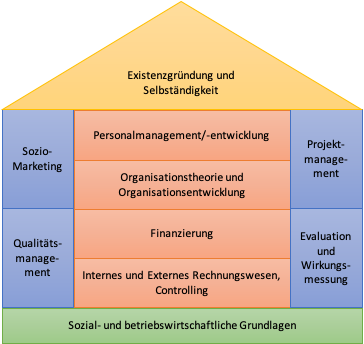
\includegraphics[keepaspectratio]{images/figure31.png}} \hfill{}

\caption{Abb. 3.1: Haus der BWL (eigene Darstellung)}

\end{figure}%

Das Fundament bilden die sozialen betriebswirtschaftlichen Grundlagen.
Hierauf wurde bereits weiter oben eingegangen und die Grundzusammenhänge
wurden schon erarbeitet.

In der Mitte des Hauses steht die rote Säule, einerseits
das~\emph{interne und externe Rechnungswesen}~und andererseits
das~\emph{Controlling}. Diese Bereiche stellen die Hard Facts und damit
gewissermaßen die zahlenmäßige Informationsbasis für wirtschaftliche
Zusammenhänge innerhalb der Einrichtung dar.
Die~\emph{Finanzierung}~wiederum ergänzt das Ganze, um eine Übersicht zu
den zur Verfügung stehenden finanziellen Mitteln, die eventuell
beschafft oder hinsichtlich ihrer Verwendung geprüft werden müssen, zu
bieten.

Dann gibt es die~\emph{Organisationstheorie und
Organisationsentwicklung}~zu betrachten. Das ist derjenige Teil, der
sich mit den organisations- und arbeitswissenschaftlichen Zusammenhängen
beschäftigt. Dabei geht es um die Frage, wer welche Aufgabe innerhalb
einer Einrichtung hat, wie sie strukturiert werden kann und wie Prozesse
verändert werden können.

Das~\emph{Personalmanagement}~beschäftigt sich mit der Frage, wie
Personen innerhalb von Einrichtungen geleitet, motiviert und geführt
werden und sich weiterentwickeln können.

Zurück zur Metapher: Das Haus hat noch Balkons: auf der linken Seite ist
das~\emph{Sozialmarketing}~zu finden. Das Sozialmarketing ist ein
spezifisches Marketing, was sich mit sozialen Einrichtungen beschäftigt.
Dabei kommen die allgemeinen Grundlagen aus der
Betriebswirtschaftslehre, die sich mit dem Marketing von Unternehmen
beschäftigen, zur Anwendung. Die allgemeinen Marketinggrundlagen müssen
aber übertragen und ggf. modifiziert werden, um sie in sozialen
Einrichtungen auch nutzen zu können.

Dann gibt es das~\emph{Qualitätsmanagement}. Dieses hat das Ziel, die
Professionalität und Qualität der Ziele und Ergebnisse sowie Strukturen
und Prozesse zu überprüfen. Des Weiteren gibt es
das~\emph{Projektmanagement}~und auch das~\emph{Change-Management}. Hier
geht es um die Frage der sinnvollen Durchführung von Projekten, deren
Planung und Umsetzung sowie deren Evaluierung und um die erfolgreiche
Organisationsentwicklung.

Schließlich gibt es noch den Bereich der~\emph{Evaluation und
Wirkungsmessung}. Das ist der Bereich, der sich mit der Wirkung von
Leistungen beschäftigt. Nicht nur im finanziellen Sinne, sondern ganz im
Gegenteil wird die Frage gestellt, welcher Beitrag geleistet wird, damit
die Qualität, also die Lebensqualität der Klient*innen verbessert wird.
Gleichzeitig stellt sich auch die Frage, wie möglicherweise Einfluss
darauf genommen werden kann, dass es in dem jeweiligen Stadtteil oder
der Region zu einer Verbesserung kommt. Wirkungsmessung in diesem
Zusammenhang bezieht sich auf die sozialen Wirkungen. Dies sind nicht
zwingend monetäre, sondern gerade auch die gesellschaftlichen
Veränderungen, die erzielt wurden: entweder durch die Tätigkeit der
Sozialarbeitenden oder durch sozialpädagogische Maßnahmen selbst.

Das Dach des Hauses könnte eigentlich auch der Keller sein: Hier
verbirgt sich das Aufgabenfeld~\emph{Existenzgründung und
Selbstständigkeit}. Es ist deswegen auf das Dach gesetzt worden, weil
hier alle Grundlagen, die vorher genannt wurden, zum Zuge kommen: Wenn
eine Einrichtung gegründet und dann die Finanzplanung gemacht werden
soll, braucht es die Finanzierung und das Rechnungswesen. Gleichzeitig
bedarf es auch der Kenntnisse des Personalwesens, Wissen über die
Strukturierung der Organisation und von einschlägigen rechtlichen
Rahmenbedingungen. Die anderen Maßnahmen, wie zum Beispiel das
Marketing, sind erforderlich, um überhaupt die Zielgruppe näher zu
bestimmen, den Markt einzuschätzen und auch die Wettbewerber
kennenzulernen. Das verstehen wir unter dem Haus der BWL.

\section{Rechnungswesen}\label{rechnungswesen}

\subsection{Überblick zum
Rechnungswesen}\label{ueberblick-zum-rechnungswesen}

Das Rechnungswesen wird auch als betriebliches Rechnungswesen bezeichnet
und hat die Aufgabe, die wirtschaftlichen Zusammenhänge in der
Einrichtung darzustellen. Hierbei sind vier Teile dieses Rechnungswesens
zu erörtern. Es gibt zwar noch weitere Teile, aber es soll hier erstmal
des Überblicks Willen um diese vier Teile gehen (vgl. im Folgenden
Arnold, 2024).

\subsubsection{Finanzierung}\label{finanzierung}

Die Finanzierung bzw. das Finanzmanagement ist eine zukunftsbezogene
Aufgabe mit dem Ziel, alle in der Einrichtung verfügbaren bzw. zu
akquirierenden Mittel zu verwalten bzw. die Zahlungsströme zu steuern.
Dadurch muss sich sodann die Zahlungsfähigkeit bestimmen lassen. Sie
lässt sich zum Beispiel mithilfe einer Liquiditätsplanung ermitteln.
Dabei werden die Einzahlungen den Auszahlungen gegenübergstellt und so
lässt sich relativ schnell erfassen, ob zusätzliche Finanzierungsmittel
notwendig sind oder ob schon mit den erwarteten Einzahlungen alle
Rechnungen beglichen werden können. Investitionsrechnung beschäftigen
sich mit der Frage, inwieweit sich Investitionen rentieren.

Wenn bspw. ein Gebäude und ein Grundstück erworben und gebaut werden
soll, dann müssen entsprechende finanzielle Mittel dafür aufgenommen
werden, z. B. durch einen Kredit. Die Frage, die sich sodann stellt,
ist, ab wann sich die eingesetzten Mittel tatsächlich rentiert haben,
also ab wann wieder positive Zahlen geschrieben werden. Bei der
Finanzierung geht es allgemein darum, wo bestimmte Mittel herkommen,
nämlich aus der Innenfinanzierung, der Außenfinanzierung, der Eigen-
oder Fremdfinanzierung. Hierbei wird danach unterschieden, ob eigene
Mittel (bspw. Einlagen von Gesellschaftern/durch Gewinnrücklagen) oder
ob Fremdmittel (bspw. Aufnahme eines Darlehens bei einer Bank)
eingesetzt werden.

\subsubsection{Finanzbuchhaltung}\label{finanzbuchhaltung}

Die Finanzbuchhaltung ist zeitraumbezogen und vergangenheitsorientiert,
womit gemeint ist, dass alles systematisch aufbereitet ist. Alle
Geschäftsvorfälle während eines Geschäftsjahres sind zu dokumentieren
und werden in Vorbereitung auf einen Jahresabschluss am Ende des Jahres
erledigt. Zum Inhalt des Jahresabschlusses: Es muss eine Bilanz
aufgestellt werden, welche die Gegenüberstellung von Vermögen und
Kapital darstellt. Darüber hinaus kann es noch andere Bestandteile
geben, wie z. B. die Gewinn- und Verlustrechnung. Hier werden die
Erträge und die Aufwendungen gegenübergstellt und somit gewissermaßen
der Erfolg am Ende des Jahres ermittelt: ein Gewinn oder Verlust.

\subsubsection{Kosten- und
Leistungsrechnung}\label{kosten--und-leistungsrechnung}

Zur Abgrenzung: Die Finanzbuchhaltung wird auch als externes
Rechnungswesen bezeichnet, die Kosten- und Leistungsrechnung als
internes Rechnungswesen. Was ist der Unterschied? Die Finanzbuchhaltung
muss gesetzlichen Auflagen folgen: dem Handels- und Steuerrecht. Danach
müssen entsprechend auch die Bilanz und die Gewinn- und
Verlustrechnungen erstellt werden. Bei der Kosten- und Leistungsrechnung
haben wir diese rechtlichen Verpflichtungen im Regelfall nicht; es gibt
Ausnahmen wie z. B. für Pflegeeinrichtungen und Krankenhäuser. Im
internen Rechnungswesen, welches gegenwarts- und zukunftsbezogen ist,
müssen die tatsächlich angefallenen Kosten und Leistungen erfasst
werden. Dies sind die im jeweiligen Unternehmen entstandenen Kosten und
Leistungen. Diese sind in Einzel- und Gemeinkosten zu unterscheiden:
Einzelkosten lassen sich direkt zu den jeweiligen Kostenträgern
zuordnen, Gemeinkosten nur indirekt. Es handelt sich dabei um allgemeine
Kosten wie z. B. Verwaltungskosten. Die Ermittlung der Selbstkosten --
das ist das übergeordnete Ziel -- geben Auskunft darüber, welche
Gesamtkosten in einer Einrichtung entstanden sind.

\subsubsection{Controlling und
Planungswesen}\label{controlling-und-planungswesen}

Dieser Bereich stellt ebenso wie das interne Rechnungswesen eine
gegenwarts- bzw. zukunftsbezogene Aufgabe dar. Hier geht es darum,
Planabweichungen möglichst rechtzeitig und früh zu identifizieren.
Hierzu werden insbesondere Budgets verwendet, um festzustellen, ob
zwischen den tatsächlich angefallenen und den geplanten Kosten eine
Abweichung vorliegt. Die Budgetierung und die anderen Instrumente dienen
letztlich dazu, eine Wirtschaftlichkeitsüberprüfung zu ermöglichen sowie
die Kosten und Gewinne innerhalb der Einrichtung zu steuern. Budgets
sind häufig mehrstufig und beinhalten Kostenstellen für die einzelnen
Teile der Einrichtung. Das Controlling dient also allgemein der
Steuerung des Unternehmens. Kurzum: das Controlling und Planungswesen
ist gewissermaßen die praktische Umsetzung der verschiedenen Zahlen, die
im Rahmen der Kosten- und Leistungsrechnung, Finanzbuchhaltung und im
Finanzmanagement ermittelt worden sind.

\subsection{Die Finanzströme eines
Unternehmens}\label{die-finanzstrme-eines-unternehmens}

Bei der Betrachtung der Finanzströme eines Unternehmens ergibt sich
meist ein komplexes Bild, wie in der folgenden Abbildung dargestellt.
Dabei steht das Unternehmen in der Mitte und es gibt verschiedene
Stakeholder, die am Unternehmen beteiligt sind oder mit diesem in
verschiedenen finanziellen Beziehungen stehen, wie z. B. die
Gesellschafter der Einrichtung, die Finanzmärkte, die Absatzmärkte und
den Staat.

Die~\emph{Gesellschafter}~haben bei Gründung der Einrichtung eine
Einlage geleistet und haben sich dadurch an der Gründung finanziell
beteiligt. Sie haben einen Anspruch darauf, dass sie an den Gewinnen
bzw. Dividenden und Einnahmen beteiligt werden. Wenn sie ihre Einlage
zurückrufen wollen, haben sie ggf. auch einen Anspruch darauf, das
Kapital zurückerstattet zu bekommen.

An den Finanzmärkten kann eine~\emph{Fremdfinanzierung}~zum Beispiel
durch Kredite und durch Darlehen aufgenommen werden. Dafür haben die
Banken oder Kreditinstitute dann ein Anspruch darauf, mindestens die
Tilgung zurückzuerhalten. Dies kann schrittweise oder auch als Ganzes
geschehen und zusätzlich haben sie noch Zinsen vereinbart, die zu zahlen
sind.

Demgegenüber können auch~\emph{Geldanlagen am Finanzmarkt}gemacht
werden, z. B. auf einem Geldmarkt- oder ein Sparkonto. Dafür können
dann, wenn die finanzielle Lage und die Märkte es hergeben, entsprechend
Guthabenzinsen erwirtschaftet werden.

Des Weiteren gibt es noch die Austauschbeziehungen mit dem~\emph{Staat}.
Bei Gründung eines Unternehmens gibt es verschiedene
Investitionszuschüsse, bei Bauprojekten z. B., oder andere Zuwendungen
aus öffentlichen Mitteln, wie z. B. von Bund, Land und Kommune. Durch
Projektmittel, die finanziert werden, oder mit den Leistungsträgern
können auch Leistungsentgelte vereinbart werden. Das sind Einnahmen, die
dem Unternehmen eine Refinanzierung ihrer Kosten ermöglichen. Darüber
hinaus muss das Unternehmen aber dennoch -- wie alle anderen Unternehmen
-- Abgaben leisten: u. a. für Sozialversicherungen, Steuern und
gegebenenfalls auch Gebühren.

Gegenüber den~\emph{Absatzmärkten}~gibt es ebenso eine
Austauschbeziehung. Dazu zählen u. a. die Klient*innen bzw. allgemein
Konsument*innen für hergestellte Güter oder angebotene Dienstleistungen.
Und diese können Privatzahlungen leisten oder es werden andere Einnahmen
generiert. Das können bspw. Umsätze aus dem Verkauf von Anlagevermögen
oder eines nicht mehr genutzten Fahrzeugs sein.

\emph{Lieferantenkredite}~sind ebenfalls eine Finanzierungsmöglichkeit,
eine Form der Fremdfinanzierung. Das ist der Fall, wenn ein Lieferant
eine Rechnung gestellt hat und diese Rechnung erst nach einer gewissen
Zeit (auf ein Zahlungsziel hin), z. B. nach 14 Tagen, beglichen werden
muss. In der Zwischenzeit können die eingekauften Waren verwendet
werden, auch wenn noch kein Cent dafür ausgegeben wurde. Des Weiteren
gibt es laufende~\emph{Auszahlungen und Anschaffungen}. Darunter fallen
Forderungen, die gegenüber den Absatzmärkten bzw. den Kunden und
Klient*innen bestehen.

\subsection{Kostenrechnung, Kostenstellenrechnung und
Kostenträgerrechnung}\label{kostenrechnung-kostenstellenrechnung-und-kostentrgerrechnung}

Schließlich wagen wir noch einen kurzen Blick in das~\emph{interne
Rechnungswesen}, welches auch als Kosten- und Leistungsrechnung
verstanden wird. Die Kosten- und Leistungsrechnung hat die Aufgaben, die
Wirtschaftlichkeit der Einrichtung zu überprüfen. Diese wird auf
unterschiedlichen sog. Rechnungsstufen unterschieden (vgl.
\hyperref[figure32]{Abb. 2.2}).\footnote{Diese Abbildung stammt aus dem
  Buch von Pelz (2004).}

\begin{figure}

\pandocbounded{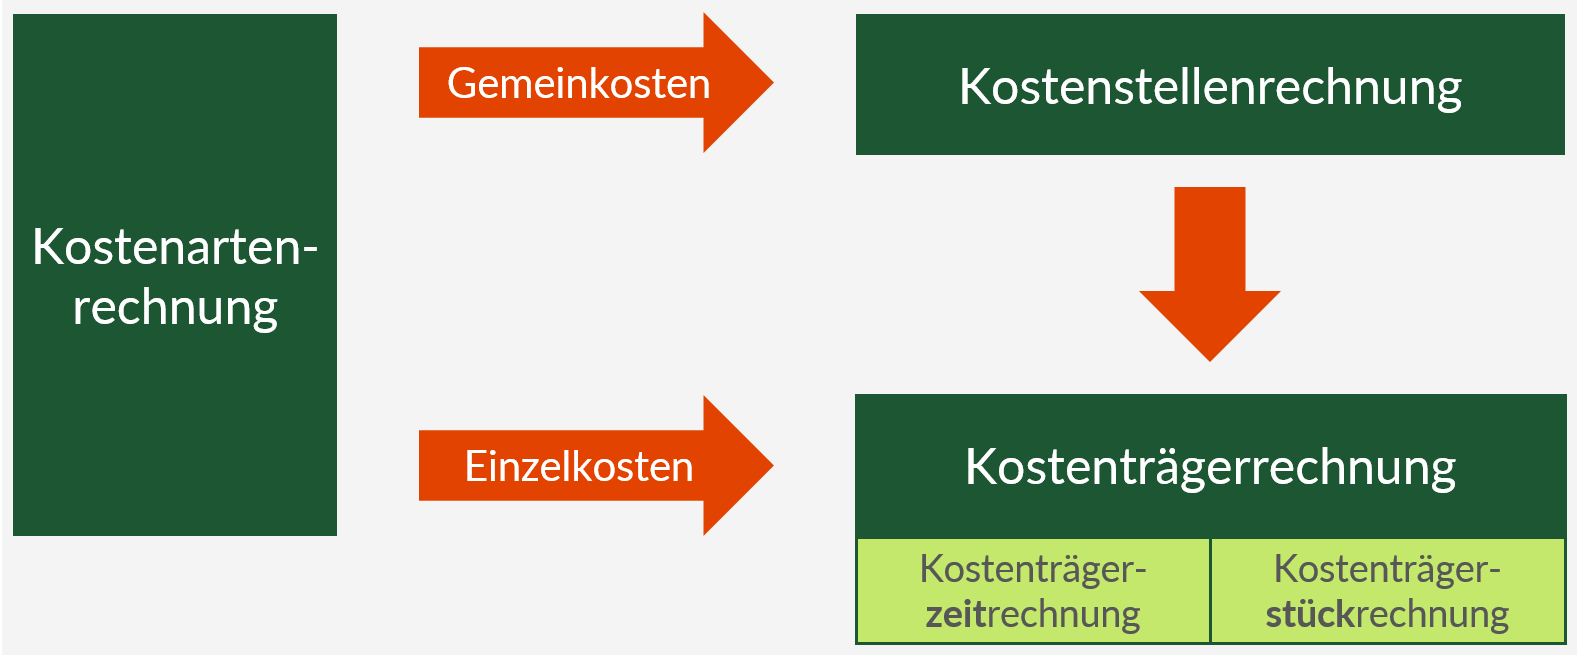
\includegraphics[keepaspectratio]{images/figure32.png}} \hfill{}

\caption{Abb. 3.2: Kostenrechnungsstufen im internen Rechnungswesen
(Trummer, o.J.). Quelle:
h\href{https://www.modu-learn.de/wordpress/wp-complete/uploads/2017/07/kostenanalyse-basis-neu.png}{ttps://www.modu-learn.de/wordpress/wp-complete/uploads/2017/07/kostenanalyse-basis-neu.png}}

\end{figure}%

Die~\emph{Kostenartenrechnung}~versucht, alle Kostenarten zu ermitteln,
, d. h. sie geht der Frage nach, welche Kosten insgesamt in der
Einrichtung anfallen. Dies sind z. B. Personalausgaben oder auch
Abschreibungen. In der~\emph{Kostenstellenrechnung}~gilt es zu
ermitteln, wo diese Kosten angefallen sind: in der Kindertagesgruppe, im
Einkauf, bei der Geschäftsleitung, in der Öffentlichkeitsarbeit oder an
sonstigen Stellen. Die~\emph{Kostenträgerrechnung}~beschäftigt sich mit
der Frage, wo die Kosten anfallen, also für welche Produkte und
Dienstleistungen. Da stellt sich die Frage, wie hoch die Kosten sind,
die im Rahmen einer Beratungsstunde, einer Betreuungsstunde oder ganz
allgemein im Rahmen eines Tagessatzes angefallen sind. Darunter lassen
sich alle Personalkosten fassen, also alle Sachkosten, die in
unterschiedlichen Kostenstellen angefallen sind. Sodann lässt sich
problemlos feststellen, wie „teuer'' eine Dienstleistung tatsächlich
ist.

\subsection{Phasen des Controllings}\label{phasen-des-controllings}

Im Controlling, wie vorangehend bereits ausgeführt, geht es um die
Aufgabe, klar zu planen und entsprechende Abweichungen frühzeitig
festzustellen, um daraus Maßnahmen abzuleiten. Hier sei ein Modell von
Bachmann (Bachmann, 2008) angeführt, der sich mit den verschiedenen
Phasen des Controllings beschäftigt (vgl. \hyperref[figure33]{Abb.
3.3}).

\begin{figure}

\pandocbounded{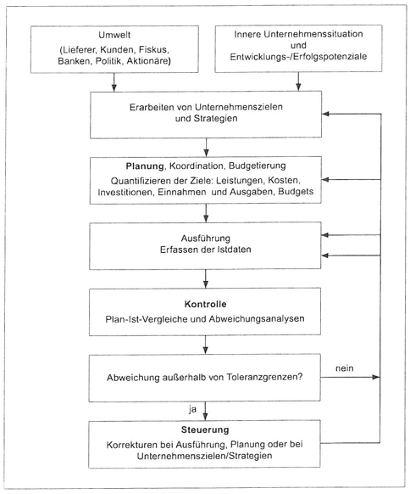
\includegraphics[keepaspectratio]{images/figure33.png}} \hfill{}

\caption{Abb. 3.3: Phasen des Controllings nach (Bachmann, 2008, S. 9)}

\end{figure}%

Neben dem Controlling müssen am Anfang erstmal eine~\emph{Umweltanalyse
sowie unternehmensinterne Analysen}~durchgeführt werden, um
herauszufinden, mit welchen Stakeholdern überhaupt eine Verbindung
besteht. Es sind die Rahmenbedingungen der jeweiligen Situation zu
beschreiben. Anschließend wird daraus ganz allgemein die Zielstellung
für die Einrichtung herausgearbeitet, sodass dies zum Beispiel in
einem~\emph{strategischen Plan}~von Jahr zu Jahr erneuert werden kann.

Nach Festlegung der Zielstellungen geht es in der nächsten Phase um
die~\emph{Planung}~einer konkreten Wirtschaftsperiode. Dies kann bspw.
im Rahmen von Budgets oder mithilfe der Budgetierung getan werden, um
damit alle Kosten und Leistungen der Einrichtung geteilt oder nach den
Einrichtungsteilen gegliedert zu ermitteln.

Schließlich müssen im Laufe des Jahres die verschiedenen tatsächlich
angefallenen Kosten erfasst werden. Diese sind tabellarisch im Budget zu
erfassen. Mit diesem Wissen ausgestattet ist man in der Lage,
die~\emph{Kontrollmaßnahmen}~durchzuführen, ob sich bspw. Abweichungen
ergeben haben oder ob überhaupt Abweichungen entstanden sind.\\
\strut \\
Sofern~\emph{Abweichungen}~entstanden sind, muss überlegt werden, ob
diese vor dem Hintergrund definierter Toleranzgrenzen tolerierbar ist.
Wenn eine Kostenstelle leicht überzogen wurde, müssen nicht gleich die
härtesten Maßnahmen, wie z. B. ein Kostenstopp für alle zukünftigen
Anschaffungen ausgesprochen werden. Lohnsteigerungen im Umfang von 2 bis
4 \% sind beispielsweise etwas Normales. Dies kann sich durch
Tarifveränderungen oder eine Steigerung der Sozialabgaben ergeben haben.

Wenn allerdings die Toleranzgrenzen überschritten sind, dann müssen
entsprechende Veränderungsmaßnahmen eingeleitet werden. Dazu dient die
letzte Phase der~\emph{Steuerung}. Hier müssen Korrekturmaßnahmen
eingeleitet werden, damit die Ziele, die ursprünglich gesetzt worden
sind, auch erreicht werden können.

An der Seite sind verschiedene Pfeile erkennbar, die andeuten sollen,
dass hier verschiedene~\emph{Feedbackprozesse}~möglich sind. In der
ersten Phase widmet man sich kurzgesagt der~\emph{Planung}. Die zweite
Phase fragt danach, wie kontrolliert werden kann
und~\emph{Abweichungen}~ermittelt werden können. In der dritten Phase
beschäftigt man sich mit den
verschiedenen~\emph{Handlungsempfehlungen}~und Instrumenten, die
aufgetretenen Abweichungen wieder zu korrigieren.

\section{Personalmanagement}\label{personalmanagement}

Management ganz allgemein bedeutet: eine zielorientierte Gestaltung und
Steuerung von Organisationen. Beim Personalmanagement bzw. in der
Personalwirtschaft geht es darum, die Einrichtung durch Maßnahmen zu
gestalten, die darauf abzielen, einerseits neues Personal zu gewinnen,
das Personal zu verwalten bzw. zu erfassen und andererseits auch für die
Personalentwicklung der Mitarbeitenden aufzukommen (z.B. (Ribbeck,
2020). Das muss hinsichtlich wirtschaftlicher, sozialer und auch
individueller Zielsetzung geschehen. Es gibt ein umfangreiches
Aufgabenpaket für das Personalmanagement (vgl. \hyperref[figure34]{Abb.
3.4}).

\begin{figure}

\pandocbounded{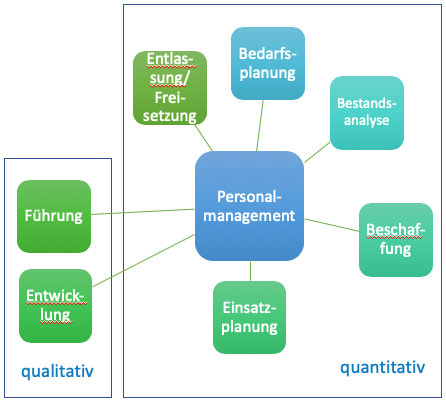
\includegraphics[keepaspectratio]{images/figure34.png}} \hfill{}

\caption{Abb. 3.4: Aufgabenfelder des Personalmanagements (in Anlehnung
an Hölzle, 2006, p. S.18)}

\end{figure}%

Zunächst gibt es die Bedarfsplanung. Mit~\emph{Bedarfsplanung}~ist
gemeint, dass man sich Gedanken machen muss, wer mit welchen Kompetenzen
in welchen Betriebsteilen zukünftig eingeplant werden soll. Das
erfordert die regelmäßige Erfassung von Personalstatistiken und das
Sammeln von personenbezogenen Daten (\emph{Bedarfsanalyse}). Die
Beschaffung -- der Begriff kommt aus der Produktionswirtschaft -- meint
hier die Akquise von Personal. Das kann von außen geschehen, das kann
aber auch intern geschehen. Außen wäre beispielsweise die
Stellenanzeige, intern eine Umsetzung oder Veränderung von
Arbeitsverträgen.

Die~\emph{Einsatzplanung}~beschäftigt sich mit der Aufgabe, kurz- bzw.
mittelfristig Dienstpläne zu erstellen. Längerfristig ist die
Einsatzplanung zum Beispiel dazu wichtig, um Karrierewege planen zu
können.

Schließlich sind gelegentlich noch \emph{Entlassungen} und
\emph{Freisetzungen} durchzuführen. Für das Personalmanagement
gesprochen, handelt es sich bei Entlassungen um die Trennung von
Mitarbeitenden. Freisetzung ist ein Sammelbegriff dafür, dass es
alternative Maßnahmen gibt, die möglicherweise eine Entlassung
verhindern können oder vermeiden lassen, wie z. B. innerbetriebliche
Versetzungen, auch Umschulungen für eine andere Stelle, Kurzarbeit oder
auch Urlaub und Sonderurlaub.

Es gibt im Personalmanagement noch die Aufgabenbereiche
der~\emph{Führung}~und~\emph{Entwicklung}. Mit Führung ist gemeint, dass
jede Leitungskraft selbst reflektieren muss und entsprechendes Wissen,
Fähigkeiten und Erfahrungen besitzen muss, ein Team zu leiten, eine
Einrichtung zu leiten und Mitarbeitende zu motivieren. Sie muss auch
selbst in der Lage sein, das eigene Leitungshandeln zu hinterfragen.
Entwicklungsaufgaben ergeben sich durch die Personalentwicklung in den
Einrichtungen, d.~h. Kompetenzen müssen ständig weiterentwickelt und
durch geeignete Maßnahmen gewährleistet werden. Darunter fallen z. B.
Personalweiterbildungen.

Das Personalmanagement kann einerseits in
einen~\emph{quantitativen}~Teil (das sind die ersten fünf aufgeführten
Bereiche) und in einen~\emph{qualitativen}~Teil unterteilt werden (z.B.
Hölzle, 2006).

\section{Organisationsentwicklung und
Change-Management}\label{organisationsentwicklung-und-change-management}

Zu diesem Funktionsbereich sei ein Modell der Organisationsentwicklung
bzw. des Change-Managements von Kurt Lewin angeführt. Dieser hat ein
Drei-Phasen-Modell entwickelt, welches mit der Metapher des Auftauens
und Einfrierens von Organisationsstrukturen argumentiert (vgl.
\hyperref[figure35]{Abb. 3.5}).

\begin{figure}

\pandocbounded{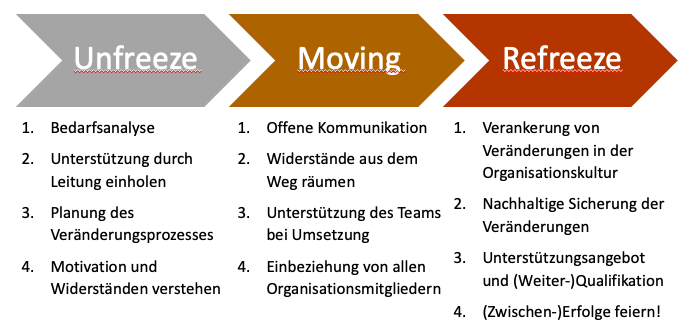
\includegraphics[keepaspectratio]{images/figure35.png}} \hfill{}

\caption{Abb. 3.5: Organisationsentwicklung und Change-Management nach
Kurt Lewins 3-Phasen-Modell (eigene Darstellung)}

\end{figure}%

In der ersten Phase, dem~\emph{Unfreezing}, geht es grundsätzlich darum,
den Bedarf und die Situation zu klären. Es muss ermittelt werden, was
verändert werden muss, wie dieser Prozess geplant werden kann, unter
welchen Umständen Mitarbeitende mitgenommen werden können und mit
welchen Widerständen ggf. gerechnet werden muss.

In der~\emph{Moving}-Phase geht es darum, offen zu kommunizieren, was
genau die Veränderung ist. Die Veränderungsprozesse müssen umgesetzt,
Widerstände behandelt und das Team regelmäßig einbezogen werden. Es sind
Fragestellungen und die dazugehörigen Lösungen zu entwickeln.
Letztendlich sollte regelmäßig über den aktuellen Stand in
Großgruppenveranstaltungen informiert werden.

In der~\emph{Refreezing}-Phase, dem Einfrieren, müssen die geänderten
Strukturen gefestigt werden. Es werden die neuen gefundenen Strukturen
und definierten Prozesse verankert. Das dient dazu, nachhaltig mit den
neuen Arbeitsstrukturen zu arbeiten und gegebenenfalls
Anpassungsqualifikationen durchzuführen. Wenn die Maßnahme erfolgreich
umgesetzt wurde, gilt es natürlich auch zum Schluss, den Erfolg zu
feiern.

\section{Sozio-Marketing}\label{sozio-marketing}

Schließlich gibt es noch den betriebswirtschaftlichen Funktionsbereich
des Marketings bzw. das~\emph{Sozio-Marketing}, also das Marketing
sozialer Einrichtungen.

\emph{Marketing}~ist zusammengefasst der Aufgabenbereich, der sich damit
beschäftigt, die jeweiligen Dienstleistungen und Produkte einerseits
hinsichtlich ihrer Qualität zu entwickeln und Werte zu schaffen sowie
andererseits zu kommunizieren sowie Kunden anzubieten und diese
Austauschbeziehung zu managen.

Nach Harald Christa (Christa, 2010) ist~\emph{Sozio-Marketing}~„auf eine
konkrete Organisation der sozialen Arbeit bzw. der Wohlfahrtspflege
bezogen'', „umfasst weit mehr als rein kommunikationspolitische
Facetten'', „Anwendung der Denkweisen undInstrumente des Marketings in
und für soziale Organisationen'' (Christa, 2010, S. 19, 24). Mithin
stellt sich die Aufgabe, die allgemeinen betriebswirtschaftlichen
Grundlagen des Marketings auf soziale Einrichtungen zu übersetzen.

Im Folgenden soll beispielhaft der \emph{Vier-Felder-Marketingmix}, ein
bekanntes Instrument des Marketings, vorgestellt werden. Dies ist dazu
geeignet, verschiedene Aufgaben bzw. Handlungsfelder des Marketings
zusammenzufassen, wobei unterschieden wird zwischen Leistungspolitik,
Preispolitik, Distributionspolitik und Kommunikationspolitik (vgl.
\hyperref[figure36]{Abb. 3.6}).

\begin{figure}

\pandocbounded{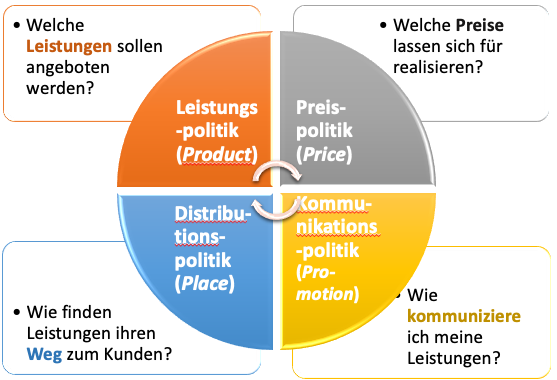
\includegraphics[keepaspectratio]{images/figure36.png}} \hfill{}

\caption{Abb. 3.6: Marketing-Mix (eigene Darstellung)}

\end{figure}%

In der~\emph{Leistungspolitik}~geht es um die Frage, welche Leistungen
überhaupt angeboten werden. Es muss ermittelt werden, wie die
marktgerechte Ausgestaltung der Leistung aussieht und welche Aussagen
sich von der Erhebung der Klient*innen- sowie Kundenbedarfe ergeben. Das
ist notwendig, um ermitteln zu können, ob die Qualität entsprechend gut
ist, sodass die Erwartungen der Kunden befriedigt werden. Des Weiteren
ist in Umwelt- oder Umfeldanalysen zu erforschen, wie sich das Produkt
bzw. die Dienstleistung von anderen unterscheidet. Eventuell ließe sich
eine Qualitäts- oder Kostenführerschaft übernehmen. Schließlich ist in
der Leistungspolitik auch eine „Unique selling proposition'' (USP) von
Bedeutung; ein Alleinstellungsmerkmal der Einrichtung muss
herausgearbeitet werden.

In der~\emph{Preispolitik}~geht es um die Frage, wie der Preis gestaltet
wird und wie sich Preise realisieren lassen. Darauf haben wir in der
Sozialwirtschaft weniger Einfluss, weil die Preise festgelegt sind, wenn
wir beispielsweise an die Leistungsentgelte denken, wobei diese Entgelte
im Regelfall feststehen. Nichtsdestotrotz müssen die Preise dahingehend
kalkuliert werden, wie z. B. durch eine Kostenanalyse soll ein Überblick
über die Kostenstruktur ermittelt werden. So muss ermittelt werden, wie
teuer eine Beratungsstunde oder ein Tagessatz ist. Wenn diese Berechnung
erfolgt ist, kann man in die Leistungsentgeltverhandlungen gehen und den
notwendigen Preis verlangen, damit alle Kosten der Einrichtung gedeckt
werden können. Es gibt ganz unterschiedliche Wege zur Preisfindung. Hier
wurde das Modell der Kostenorientierung vorgestellt. Man kann sich aber
auch bspw. bei der Kalkulation von Weiterbildungen an der Konkurrenz
orientieren. Man kann sich auch anhand der Nachfrage orientieren, also
dem Nutzer der jeweiligen Dienstleistungen. Darüber hinaus gibt es noch
das Target Costing, also die ziel- und nutzenorientierte Ermittlung von
Kosten bzw. Preisen. Die letztgenannten Verfahren sind eher im
Weiterbildungs- bzw. allgemein im Bildungsbereich passend.

Die~\emph{Distributionspolitik}~fragt danach, auf welchem Wege die
Leistungen zum Kunden gebracht werden. Es gibt sog. Absatzmittler wie z.
B. Schuldnerberatungen, die manchmal ein erster Anlaufpunkt für Menschen
in besonderen, finanziellen wie persönlichen Lebenslagen sind. Sie
können Menschen an andere Beratungen verweisen. Darüber hinaus gibt es
die Meinungsführer („Influencer''). Das sind diejenigen
meinungsbildenden Personen, die die Einrichtung kennen und
weiterempfehlen. Das können beispielsweise Selbsthilfegruppen, Elternrat
und Elterngruppen, aber auch andere Vereinigungen bzw.
Wohlfahrtsverbände sein, die auf unsere Einrichtung hinweisen. Die
Standortwahl ist ebenso ein Aspekt in Distributionspolitik. Es ist dabei
zu analysieren, wo sich die Einrichtung befindet: in einer Randlage oder
im Stadtzentrum. Davon hängt ab, welche Personen sie erreichen kann.
Schließlich sind die Öffnungszeiten sowie die Erreichbarkeit mit
öffentlichen Verkehrsmitteln entscheidend.

Den letzten großen Teil des Marketing-Mix stellt
die~\emph{Kommunikationspolitik}~dar. Hier geht es um die Frage, wie die
Leistungen kommuniziert werden können, sodass sie dann entweder die
gesamte Bevölkerung erreichen oder gezielt einzelne Gruppen ansprechen.
Es geht um die Erhöhung des Bekanntheitsgrades der Einrichtung in der
Öffentlichkeitsarbeit. Im Rahmen der Werbung müssen die
unterschiedlichen Kanäle und Medien gewählt werden: ob über Social
Media, über Werbung, über direkten Kontakt oder über eine Website.
Herausgearbeitet werden muss, mit welcher Botschaft man die Personen
erreicht, die man ansprechen will.

\section{Weitere Funktionsbereiche}\label{weitere-funktionsbereiche}

Abschließend ist ein Überblick über weitere Funktionsbereiche zu geben,
gewissermaßen die Balkone und das Dach des Hauses der BWL. Hierzu
erfolgt nur eine sehr sporadische Zusammenfassung in der folgenden
Abbildung. All diese Bereiche, die hier aufgeführt sind, haben eine
separate Veranstaltung im Laufe Ihres Studiums (vgl.
\hyperref[figure37]{Abb. 3.7}).

\begin{figure}

\pandocbounded{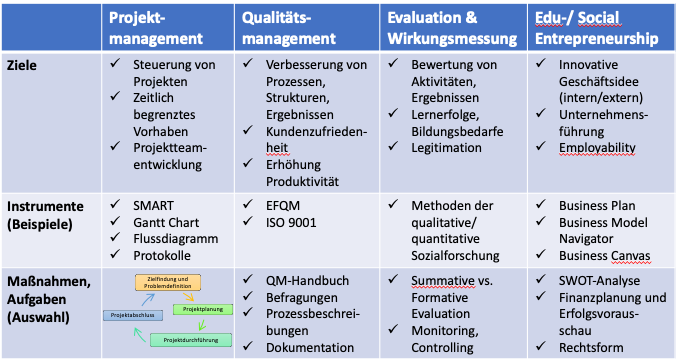
\includegraphics[keepaspectratio]{images/figure37.png}} \hfill{}

\caption{Abb. 3.7: Überblick weitere Bereich des Bildungsmanagements
(eigene Darstellung)}

\end{figure}%

Das~\emph{Projektmanagement}, darauf wurde bereits eingegangen, hat die
Aufgabe, Projekte zu steuern bzw. das Projektteam zu führen. Dabei
handelt es sich um befristete Maßnahmen. Am Anfang muss man sich
Gedanken über die Ziele zum Projekt machen. Es muss ein Plan entwickelt
werden, dieser umgesetzt sowie durchgeführt werden. Zum Schluss werden
die Ergebnisse veröffentlicht bzw. daraus ergibt sich möglicherweise ein
neues Thema, was in einem anderen Projekt umgesetzt werden kann. Die
smarte Zielformulierung kann hier als Instrument eingesetzt werden.
Ebenso können Charts dazu dienen, einen Projektplan zu entwickeln, aus
dem hervorgeht, zu welchem Zeitpunkt wann wer welche Tätigkeiten
übernimmt. Flussdiagramme sind hilfreich, um Prozesse zu beschreiben.
Zudem sind Protokolle von Meetings anzufertigen.

Das~\emph{Qualitätsmanagement}~hat die Aufgabe, Prozesse, Strukturen und
Ergebnisse regelmäßig zu überprüfen. Es bildet gewissermaßen einen
Garanten, um Standardisierung oder Professionalisierung zu ermöglichen.
In dessen Rahmen ist regelmäßig danach zu fragen, wie sich die
Kundenzufriedenheit darstellt und ob sich diese verändert hat. Umfassend
muss geprüft werden, wie die gesamte Einrichtung noch effektiver und
produktiver werden kann. Dazu gibt es verschiedene Modelle wie z. B. das
EFQM-Modell oder die DIN-ISO-Norm. Im Bereich der Sozial- und
Gesundheitswirtschaft gibt es noch zahlreiche andere Modelle und
Instrumente, die eingesetzt werden können. Im Qualitätsmanagement werden
verschiedene Maßnahmen festgelegt, Prozesse beschrieben und
dokumentiert, zudem sollte auch ein Qualitätsmanagement-Handbuch
entstehen.

Die~\emph{Evaluation bzw. Wirkungsmessung}~fragt danach, wie die
Aktivitäten und Ergebnisse, die sich im Rahmen der Tätigkeiten ergeben
haben, bewertet werden können. Zu ermitteln ist, was die Wirkungen sind,
die sich daraus ergeben und welche Effekte sich auf sozialer,
organisationaler und möglicherweise kommunaler sowie Sozialraumebene
ergeben. Sie dienen dazu, Lernerfolge, Bildungsbedarf und -veränderung
sowie Kompetenzentwicklungen abzubilden. In diesem Bereich nutzt man
Methoden der qualitativen und quantitativen Sozialforschung, um genau
diese Ergebnisbewertungen vorzunehmen. Die Evaluation hat das Ziel,
herauszufinden, wie die Ergebnisse der jeweiligen Maßnahme gegenüber
ihren Zielen zu einer wirkungsvollen Veränderung geführt haben. Die
formative Evaluation beschäftigt sich mit der schrittweisen und
begleitenden Evaluation und versucht, im Prozess eines Programms, einer
Maßnahme oder eines Projektes entsprechend durch Feedback und
Reflexionsmöglichkeiten auf den Verlauf von Monitoring- und
Controlling-Maßnahmen Einfluss zu nehmen. Die summative Evaluation
ermittelt die Wirkung nach Abschluss der Maßnahme.

Die~\emph{Evaluation bzw. Wirkungsmessung}~fragt danach, wie die
Aktivitäten und Ergebnisse, die sich im Rahmen der Tätigkeiten ergeben
haben, bewertet werden können. Zu ermitteln ist, was die Wirkungen sind,
die sich daraus ergeben und welche Effekte sich auf sozialer,
organisationaler und möglicherweise kommunaler sowie Sozialraumebene
ergeben. Sie dienen dazu, Lernerfolge, Bildungsbedarf und -veränderung
sowie Kompetenzentwicklungen abzubilden. In diesem Bereich nutzt man
Methoden der qualitativen und quantitativen Sozialforschung, um genau
diese Ergebnisbewertungen vorzunehmen. Die Evaluation hat das Ziel,
herauszufinden, wie die Ergebnisse der jeweiligen Maßnahme gegenüber
ihren Zielen zu einer wirkungsvollen Veränderung geführt haben. Die
formative Evaluation beschäftigt sich mit der schrittweisen und
begleitenden Evaluation und versucht, im Prozess eines Programms, einer
Maßnahme oder eines Projektes entsprechend durch Feedback und
Reflexionsmöglichkeiten auf den Verlauf von Monitoring- und
Controlling-Maßnahmen Einfluss zu nehmen. Die summative Evaluation
ermittelt die Wirkung nach Abschluss der Maßnahme.

In dieser Grundlagenveranstaltung wurden ausgewählte Funktionsbereiche
dargestellt, die in jeder Einrichtung eine Rolle spielen, unabhängig
davon, ob es sich um eine soziale oder um eine erwerbswirtschaftliche
Einrichtung im weitesten Sinne handelt.

\part{Ausgewählte Themenfelder}

\chapter{Was ist eine Organisation?}\label{was-ist-eine-organisation}

Im Folgenden werden wir uns mit dem organisationsbezogenen Management
beschäftigen und im Anschluss daran setzen wir uns mit verschiedenen
Managementkonzepten im Sozialmanagement (Teil 5) auseinander, die sich
insbesondere aus der öffentlichen Betriebswirtschaftslehre und dem
Non-Profit-Management ableiten lassen. Zunächst ist aber zu klären, was
Organisationen eigentlich sind und wie man diese sozialen Gebilde
beschreiben kann. Natürlich gibt es ganz unterschiedliche
Herangehensweisen und Aspekte, die wir einer Organisation bzw.
Organisationen zuschreiben können. Ein Aspekt der Organisation ist die
Koordination des Zusammenwirkens und die Ermöglichung einer inneren
Ordnung, wie unter anderem ihr Aufbau oder ihre Struktur. Prozesse
müssen definiert werden, es gibt feste Abläufe, es gibt
Verantwortlichkeiten und vieles mehr, das uns ermöglicht, koordinativ
zusammenzuwirken.

Darüber hinaus gibt es noch eine zweite Eigenschaft. Wir können
Organisationen als soziales System betrachten, die in einer Gesellschaft
ein Eigenleben besitzen. D. h. wenn eine Organisation gegründet wurde,
dann ist sie ein eigenes Objekt, ein abstraktes Gebilde, das in die Welt
gebracht wurde, welches wir für die Koordination nutzen können. Und man
kann es vielleicht daran erkennen, dass Organisationen bzw. Firmen
(rechtsdeutsch) auch Namen haben. Wir geben einer Organisation also
einen Namen, machen sie dadurch „persönlicher'' und direkter. Darüber
hinaus ist noch ein dritter Aspekt wichtig, wenn wir über Organisationen
sprechen: sie sind soziale Gebilde, die ein bestimmtes oder auch mehrere
Ziele verfolgen können. D. h. Organisationen ermöglichen ein
zielgerichtetes Handeln.

Stellen wir uns im Weiteren die Frage, was denn eine Organisation ist
bzw. was Organisationen ausmachen: Organisationen an sich umfassen
erstens eine Mehrzahl an Personen, die in dieser zusammenarbeiten. Der
Begriff ist so essenziell, dass wir häufig nach Synonymen ringen müssen,
weil wir einerseits Organisationen als Gebilde betrachten können, also
als abstrakte Einheiten. Andererseits ist die Organisation auch eine
Tätigkeit, nämlich etwas „zu organisieren'', z. B. die Durchführung
eines Projekts. Darüber hinaus kann man auf die Idee kommen, dass die
Menschen, die in Organisationen zusammenarbeiten, häufiger ihre Arbeit
im Sinne einer funktionalen Arbeitsteilung verrichten und eine
Organisation überhaupt erst eine Grundlage dafür schafft, dass man die
einzelnen Arbeitsprozesse aufeinander abstimmen und gleichzeitig
verschiedene Ziele verfolgen kann. D. h. es sind nicht nur mehrere
Personen, die zusammenarbeiten, sondern es gibt auch eine Koordination
der Zusammenarbeit. Zudem besitzen Organisationen jeweils eine Struktur
bzw. Hierarchie, die festgelegt werden muss. Es muss hierbei geklärt
werden, wer für was zuständig ist und entsprechend wer welche
Verantwortung(en) übertragen bekommt.

Schließlich kann man festhalten, dass Organisationen so etwas wie
soziale Systeme sind. Der Systembegriff taucht in ganz verschiedenen
Zusammenhängen im Laufe des Studiums der Sozialpädagogik und des
Sozialmanagements an mehreren Stellen auf. Letztgenannter Begriff hilft
zu beschreiben, wie Menschen miteinander zusammenwirken und wie
Zusammenarbeit überhaupt erst ermöglicht wird. Ich möchte erinnern an
die Unterschiede und Gemeinsamkeiten von Non-Profit- und
For-Profit-Organisationen nach Schwarz (1986), wo ebenfalls erwähnt
wurde, dass jede Organisation eine Art soziales System darstellt.

\section{Eigenschaften und Funktionen von
Organisationen}\label{eigenschaften-und-funktionen-von-organisationen}

Organisationen haben ganz verschiedene Funktionen. Sie dienen einerseits
der Überlebenssicherung, da sie für einen bestimmten Zweck gegründet
werden, um ein Ziel zu verfolgen; sie leisten damit für eine
Gesellschaft einen konkreten Beitrag in der Umsetzung bestimmter
Aufgaben. Darüber hinaus dienen sie dazu, wie oben bereits erwähnt, das
Zusammenleben zu organisieren und zu ordnen. Mit anderen Worten:
Organisationen werden ins Leben gerufen, um komplexe Problemstellungen
zu lösen, wozu eine Einzelperson möglicherweise nicht in der Lage wäre.

Gleichzeitig fungieren Organisationen bzw. ihre rechtsverbindlichen
Vertreter*innen häufig auch als Arbeitgeber und durch einen
Arbeitsvertrag wird das Überleben bzw. die Existenz der Mitarbeitenden
gesichert. Durch Organisationen wird also Arbeitsteilung ermöglicht.
Darüber werden Organisationen selbst als Objekte, als Entitäten
wahrgenommen, die mit anderen Organisationen zusammenarbeiten, etwa auf
Basis von Kooperationsverträgen. Sie treten dabei als Vertragspartner
auf, wenn sie eine eigene Rechtspersönlichkeit (= juristische Person,
gegenüber sog. natürlichen Personen nach Privat- oder öffentlichem
Recht) besitzen, z. B. Verein, Stiftung, GmbH.

Organisationen haben eine eigene Identität bzw. Persönlichkeit, die es
ermöglicht -- zumindest theoretisch -- eine Grenze zwischen dem Außen
und dem Innen zu ziehen. Nach außen hin erfolgt eine Abgrenzung zum
Wettbewerb und zu anderen nicht der Einrichtung Angehörigen. Nach innen
hin erfolgt es eine Sinngebung bzw. Zwecksetzung. Hier wird mit der
Organisation ein „Wir'' geschaffen. Dabei ist zu betonen, dass das Wir
ja durch einen Zusammenschluss von mehreren Menschen entstanden ist. Das
Wir bildet eine gewisse Gruppenidentität.

Menschen können ganz unterschiedliche Beziehungen zu Organisationen
aufbauen, z. B. können sie einer Organisation angehören. Damit werden
sie zu Mitgliedern der Organisation. Darüber hinaus gibt es aber auch
eine andere interessante Eigenschaft: Organisationen koordinieren auch
Menschen, z. B. indem bestimmte Ziele verfolgt und festgelegt werden,
was dazu führt, dass bestimmte individuelle Interessen bisweilen auch
zurückgesteckt werden müssen und dann sozusagen die Organisationsziele
im Vordergrund stehen.

Menschen passen sich in Organisationen über verschiedene Rollen und
Regeln an. Dann stellen sich Fragen wie z. B.: Was ist das richtige bzw.
anpasste Verhalten? Wie gehen wir aufeinander zu? Wie kommunizieren wir
mit unseren Stakeholdern? Was gibt es für Spielräume bzw. informelle
Regeln, die es zu beachten gilt? All das gehört u. a. zur
Organisationsstruktur und Organisationskultur, womit wir uns später
beschäftigen werden. Schließlich haben Organisationen, wie bereits
erwähnt, ein übergeordnetes Ziel: sie verfolgen eine Zweckrationalität.
Rationalität wird von ratio (lat. „Vernunft'', „Methode'') abgeleitet.
Zweckrationalität meint das Einrichtungsziel bzw. den Zweck der ggf. in
der Satzung einer Einrichtung definiert ist. Alle einer Organisation
angehörigen Mitglieder richten ihr Verhalten an den vorhandenen
Verantwortlichkeiten und Machtstrukturen aus. Solche Hierarchien werden
z. B. in Organigrammen festgelegt. Es gibt Befugnisse, die ausgesprochen
werden, und darüber hinaus ist natürlich auch die Verwirklichung der
persönlichen Ziele, Ideen und Interessen der Mitglieder von Bedeutung,
insbesondere wenn die eigenen Kompetenzen, Wissen und Fähigkeiten
weiterentwickelt werden sollen. Also kurz zusammengefasst geht es hier
darum, den Zweck und die Rationalität, für die die Einrichtung steht, zu
verwirklichen.

\section{Bilder von Organisationen}\label{bilder-von-organisationen}

Schauen wir uns im Folgenden verschiedene Bilder von Organisationen an.
Ich gehe hier auf einen Ansatz von Gareth (Morgan, 1986; dt. Morgan,
1997) zurück, der in seinem gleichnamigen Buch Ende der 1980er Jahre von
den ``Images of Organization'' gesprochen hatte. Zur Darstellung der
Geschichte der Organisationstheorie hat Morgan Metaphern verwendet. Vier
dieser Bilder, die unmittelbar interessant für unser Veranstaltungsthema
sind, seien im Folgenden einmal herausgegriffen, da sie uns ein besseres
Verständnis dafür liefern, wie sich die Idee von Organisationen im
Zeitverlauf entwickelt hat.

Erstens können Organisationen als Maschinen betrachtet werden. Hier
befinden wir uns im Zeitalter der Industrialisierung. Organisationen
sind Großunternehmen, die Massenprodukte in Fließbandarbeit herstellen.
Maschinen müssen regelmäßig geölt werden, um stets wie zwei Zahnräder
ineinandergreifen zu können. Eine Organisation funktioniert nur dann,
wenn auch das Räderwerk läuft. Diesem Bild einer Organisation liegt ein
mechanistisches Weltbild zugrunde, das natürlich dann später auch
kritisiert worden ist, z. B. mit Hilfe der Systemtheorie.

Organisationen können zweitens auch als Organismen bzw. lebende Systeme
angesehen werden. Damit ist gemeint, dass, wie im menschlichen Körper
bzw. anderen komplexen Organismen, die einzelnen Organe und Zellen
koordiniert miteinander zusammenarbeiten. Nicht jede Zelle hat die
gleiche Aufgabe, sondern es gibt ganz unterschiedliche Aufgaben, die von
Spezialisten in einem arbeitsteilig organisierten, wechselseitig
vernetzten System miteinander umgesetzt werden. Hier ist eine ganz
andere Metapher im Spiel, nämlich eine biologistische Sichtweise auf
Organisationen, was letztlich auch einen Ursprung der für die später
beschriebene Systemtheorie darstellt (z. B. Kybernetik). Im
metaphorischen Sinn des Organismus werden Organisationen als
funktionsfähige, soziale Systeme betrachtet.

Drittens können Organisationen auch mit der Metapher ‚Kultur'
beschrieben werden. Diese anthropologische, sozial- und
kulturwissenschaftliche Sichtweise besagt, dass Organisationen auf Basis
bestimmter Regeln, Werte und Normen aufgebaut sind und ihre Mitglieder
verschiedene soziale und funktionale Rollen einnehmen können. Letztlich
kann damit alle Eigenschaften, die allgemein dem abstrakten Phänomen
‚Kultur' zugeordnet werden können, auch auf das Zusammenwirken von
Menschen in Organisationen übertragen werden, z. B. dass die Mitglieder
in Organisation durch die Organisationskultur geprägt werden,
gleichzeitig aber auch die Mitglieder die Organisationskultur
entscheidend mitprägen.

Viertens können Organisationen auch im Sinne eines (psychischen)
Gefängnisses verstanden werden. Hierbei liegt eine psychoanalytische
Sichtweise zugrunde. Damit ist gemeint, dass alle Mitglieder einer
Organisation bestimmte Bedürfnisse und Befindlichkeiten, wie z. B.
Bedürfnisse nach Sicherheit, Anerkennung und Beteiligung, haben.
Insbesondere dann, wenn sich einzelne Individuen nicht unmittelbar mit
den organisationalen Zielen identifizieren können, z. B. weil es
persönliche Vorbehalte oder widersprüchliche Auffassungen gibt, kann
eine Organisation möglicherweise auch etwas erdrückend wirken.
Individuelle und organisationale Ziele können dabei nicht gleichzeitig
erreicht werden.

\section{St.~Galler Management-Modell der 3. Generation und seine
Erweiterungen}\label{st-galler-management-modell-der-3-generation-und-seine-erweiterungen}

\subsection{St.~Galler Management-Modell der 3. Generation nach
Rüegg-Stürm
(2003)}\label{st.-galler-management-modell-der-3.-generation-nach-ruxfcegg-stuxfcrm-2003}

In diesem ganzheitlichen und systemorientierten Modell wird eine
Organisation bzw. ein Unternehmen eingebettet in Ihrer Systemumwelt
dargestellt (vgl. Rüegg-Stürm, 2003). Das Modell ist wie in
\hyperref[figure41]{Abb. 4.1} aufgebaut.

\begin{figure}

\pandocbounded{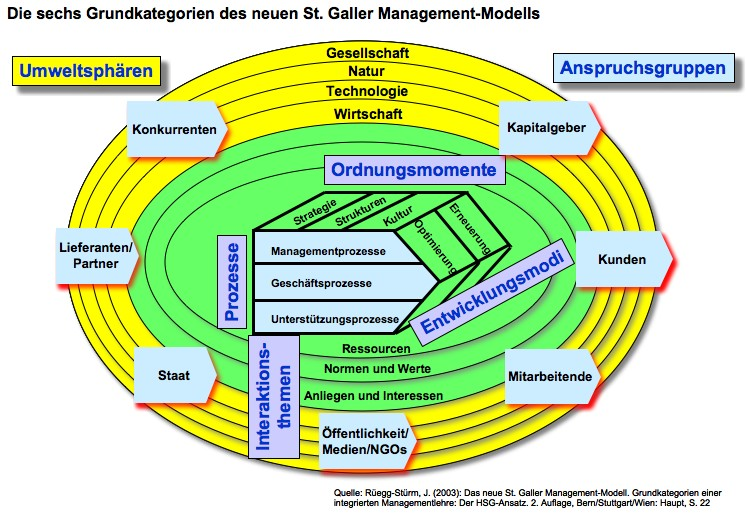
\includegraphics[keepaspectratio]{images/figure41.jpeg}} \hfill{}

\caption{Abb. 4.1: Grundkategorien des SGMM (Rüegg-Stürm, 2003, S. 22),
Quelle: \url{https://de.wikipedia.org/wiki/Datei:SGMM2.jpg} (CC Public
Domain)}

\end{figure}%

Auf den äußeren Schalen gibt es die sog. Umweltsphären. Dies bilden die
Rahmenbedingungen, in denen sich Organisationen bewegen und bewähren
müssen. Dazu gehören beispielsweise gesellschaftliche Prozesse, z. B.
Teilhabe, Partizipation und Sozialgesetzgebung, ebenso aber auch die
natürlichen (z. B. nachhaltiges Wirtschaften), technologischen und
wirtschaftlichen Rahmenbedingungen bzw. die Sozialwirtschaft im Ganzen
gesehen. In diesen Umweltsphären und mit der Organisation unmittelbar in
Beziehung stehend gibt es verschiedene Anspruchsgruppen, die sogenannten
Stakeholder.

Bei den Stakeholdern kann es sich um Einzelpersonen oder auch Gruppen
handeln. Der Staat gibt bspw. die gesetzlichen Rahmenbedingungen vor,
nach denen wir uns zu orientieren haben. Die Lieferanten stellen uns
bestimmte Produkte oder auch Dienstleistungen zur Verfügung, sodass eine
Einrichtung überhaupt erst einmal betrieben kann. Organisationen stehen
darüber hinaus in Konkurrenz bzw. Wettbewerb mit anderen Einrichtungen,
die ähnliche Produkte und Dienstleistungen anbieten. Bei den
Kapitalgebern können wir etwa an die Leistungs- bzw. Kostenträger in der
Sozialwirtschaft denken, die soziale Dienstleistungen finanzieren. Es
gibt Kund*innen bzw. Klient*innen, für die wir unsere Dienste anbieten
und schließlich gibt es die Mitarbeitenden, die innerhalb einer
Einrichtung dafür verantwortlich sind, dass der Zweck verfolgt wird,
alle notwendigen Aufgaben erledigt und die Qualität des Angebots
weiterentwickelt wird. Eine Austauschbeziehung besteht regelmäßig auch
mit der Öffentlichkeit, den Medien und Nichtregierungsorganisationen (z.
B. Gewerkschaften). Alle diese Stakeholder haben verschiedene Aufgaben
bzw. tragen verschiedene Interessen und Erwartungen an die Einrichtung
heran. Dies wurde bereits weiter oben bei dem Konzept der
Multirationalität angesprochen. Mit anderen Worten handelt es sich bei
dem St.~Galler Management-Modell um ein stakeholderorientiertes Konzept.

In der Mitte der Grafik befindet sich schließlich die Organisation
selbst, die über sog. Interaktionsthemen, dargestellt auf den inneren
Kreisen, mit den Stakeholdern verbunden sind. Zu diesen Austauschthemen
gehören bspw. Ressourcen, Normen und Werte sowie Anliegen und
Interessen. Mit Ressourcen ist gemeint, dass hier sozusagen personelle,
finanzielle und sachliche Ressourcen zur Verfügung gestellt werden
müssen, damit die Einrichtung funktioniert. Denn jede Einrichtung
benötigt Personal und finanzielle Mittel, Gerätschaften, ein Gebäude
bzw. Räumlichkeiten. Darüber hinaus gibt es Normen und Werte, die
grundlegend für die Zusammenarbeit gelten, z. B. professioneller
Anspruch gegenüber den Klient*innen, Kommunikationsregeln innerhalb der
Einrichtung. Außerdem gibt es verschiedene Anliegen und Interessen der
einzelnen Stakeholder, die aufgenommen bzw. bearbeitet werden müssen, z.
B. finanzielle Interessen, Kooperationen mit anderen Einrichtungen,
Kompetenzentwicklung der Mitarbeitenden.

Im Mittelpunkt der Grafik steht die als Pfeil dargestellte Organisation
selbst, dort werden die sog. Ordnungsmomente beschrieben, u. a.
Organisationsstrategie, Organisationsstruktur und die
Organisationskultur. Auf der Strategieebene geht es um die allgemeinen
und spezifischen Zielsetzungen und strategische Pläne innerhalb von
Organisationen. Mit Hilfe der Organisationsstruktur wird die Frage
geklärt, wie Organisationen aufgebaut sein müssen, z. B. in Form eines
Organigramms. Bei der Organisationskultur steht die Frage im
Vordergrund, wie wir in der Einrichtung miteinander zusammenarbeiten,
welche Werte wir teilen und welche Gepflogenheiten und Verhaltensweisen
existieren. Auf der Vorderseite des als Pfeil dargestellten Unternehmens
sehen wir verschiedene Prozesse, die innerhalb von Organisationen
ermöglicht werden sollen. Dazu gehören Managementprozesse, wozu
verschiedene Leitungs- und Führungsaufgaben wie Personalentwicklung,
Controlling und Geschäftsführung zählen. Die Geschäftsprozesse umfassen
demgegenüber alle alltäglichen Aufgaben bis hin zur Tagesplanung. Mit
Unterstützungsprozessen sind solche Prozesse gemeint, die die
Einrichtung in die Lage versetzen, den alltäglichen Betrieb zu
organisieren, z. B. Reinigungsdienste und Essensversorgung.

An der Pfeilspitze gibt es die sog. Entwicklungsmodi. Damit ist gemeint,
dass sich jede Organisation kontinuierlich weiterentwickeln muss. Dies
kann durch Erneuerungs- und Optimierungsprozesse geschehen. Optimierung
heißt, dass man dabei einerseits kleine Schritte gehen und Schritt für
Schritt Veränderungen umsetzen kann, während die Erneuerung eine
radikale Unternehmenstransformation darstellt, welche möglicherweise mit
Brüchen und einer neuen Unternehmensphilosophie einhergehen kann.

Alle weiteren Ausführung in diesem Abschnitt des organisationsbezogenen
Managements sind entsprechend der verschiedenen Ebenen und Aspekte des
St.~Galler Management-Modells der dritten Generation strukturiert.
Ausführlicher wird sich dann mit dem Strategieprozess, der Struktur- und
Prozessperspektive, Organisationskultur und der Organisationsentwicklung
beschäftigt.

\subsection{Systemisch-reflektiertes Management-Modell nach Lambers
(2015)}\label{systemisch-reflektiertes-management-modell-nach-lambers-2015}

Eine Erweiterung bzw. Übersetzung des St.~Galler Management-Modells
dritter Generation hat Lambers (Lambers, 2015) in Form seines sog.
\emph{Systemtheoretisch-reflektierten Managementmodells (SRM)}
vorgenommen. Dabei wurde versucht, das Modell für soziale Einrichtungen
zu konkretisieren. Auf der äußeren Schale, der Umweltsphären, sind
verschiedene Rahmenbedingungen und Kontexte der Sozialen Arbeit
hervorgehoben, z. B. Familie, Politik, Recht, Erziehung, Medien,
Massenmedien, Wissenschaft und Wirtschaft. Diese bilden gewissermaßen
die Grundkontexte und Ausgangsbedingungen, in denen sich soziale
Organisation befinden bzw. bewähren müssen. Der innere, dunkelgrau
dargestellte Kreis beinhaltet die verschiedenen Normen, Werte,
Ressourcen und Interessen, welche für den Austausch zwischen den
verschiedenen Stakeholder und der Einrichtung von Bedeutung sind: z. B.
Geschäftsführung, Aufsichtsorgane, Netzwerke, Kooperationspartner,
Konkurrenten, Aufsichtsbehörden, Kosten- bzw. Leistungsträger. Außerdem
gibt es noch andere Adressaten, Angehörige, Berater*innen und
Mitarbeitende, die als Stakeholder eine bedeutende Rolle spielen können.
Mit der Blackbox ist gemeint, dass es möglicherweise noch weitere
Beteiligte geben kann, die uns aber aktuell nicht bekannt sind und ggf.
mit einer Stakeholderanalyse erst ausfindig gemacht werden müssen. Im
Zentrum des Modells steht wie auch im Originalmodell die Organisation
selbst. Die Ordnungsmomente sind gleich dargestellt. Neu sind neben den
Management-, Geschäfts- und Unterstützungsprozessen die sog.
Vernetzungsprozesse. Damit ist gemeint, dass es auch zur allgemeinen
Aufgabenstellung für Einrichtungen der sozialen Arbeit gehört, die
Vernetzung zwischen und mit anderen Einrichtungen herzustellen und zu
pflegen, z. B. Grundschule, Hort und Kita.

\section{Strategieebene}\label{strategieebene}

\subsection{Strategieentwicklung}\label{strategieentwicklung}

Im Folgenden betrachten wir zunächst einmal detaillierter das
Ordnungsmoment der Strategieentwicklung. Insbesondere gehen wir dabei
auf das Leitbild als Bestandteil der strategischen
Unternehmensentwicklung ein. Nach Giesel (2007) kann der
Strategieentwicklungsprozess anhand der Ebenen normatives, strategisches
und operatives Management beschrieben werden. Auf der normativen
Managementebene wird die unmittelbare Zwecksetzung der Einrichtung
festgelegt, warum und für was die Einrichtung gegründet wurde. Die
strategische Ebene beschäftigt sich mit der Frage, welche Ziele denn
formuliert werden müssen, damit die Unternehmensphilosophie bzw. die
Zweckbestimmung der Einrichtung überhaupt sinnvoll erreicht werden kann.
Das operative Management auf der untersten Ebene ist gewissermaßen das
Alltagsgeschäft. Dabei geht es darum, die gesetzten Ziele umzusetzen, um
dann am Ende des Jahres zu überprüfen, ob die Ziele schließlich erreicht
worden sind.

Den einzelnen Managementebenen lassen sich schließlich die verschiedenen
Aufgaben im Rahmen der Strategieentwicklung zuordnen. Auf normativer
Ebene muss die Unternehmensphilosophie und Unternehmenspolitik, also das
grundlegende Ziel formuliert werden. Das Leitbild, in der Mitte als
Pfeil dargestellt, bildet gewissermaßen das grundlegende Konzept bzw.
das integrative Verbindungsglied zwischen dem normativen, strategischen
und operativen Management. Auf normativer Ebene wird festgelegt, was die
vertretenen Werte und Überzeugungen der Organisation sind, welche
Aufträge verfolgt werden, wie die Zusammenarbeit gestaltet werden soll.
Auf strategischer Ebene muss in Programmen konkretisiert werden, wie die
Unternehmensphilosophie in der jeweiligen Planungsperiode umgesetzt
werden soll. Die Organisation hat verschiedene Aufträge zu erfüllen und
in Form von sog. Programmen bzw. Plänen ist längerfristig der
Arbeitsprozess und die Geschäftsentwicklung zu planen. Für die
Wirtschaftsplanung kann man sich hier beispielsweise die Aufstellung
eines Planbudgets vorstellen, was die Bewirtschaftung aller verfügbaren
Ressourcen beinhaltet, die zur Verwirklichung der Strategien dienen
können. Schließlich auf der untersten Ebene müssen die einzelnen
Aktivitäten, die einzelnen Prozesse, ob dies nun Management-,
Geschäfts-, Unterstützungs- oder Vernetzungsprozesse sind, für die
jeweiligen Planungsperiode organisiert werden.

\subsection{Leitbilder}\label{leitbilder}

\subsubsection{Funktionen von
Leitbildern}\label{funktionen-von-leitbildern}

Das Leitbild beschreibt den Auftrag bzw. die Vision einer Einrichtung:
Für welche Zwecke sind wir gegründet worden, wer arbeitet in unserer
Einrichtung, welche Werte verfolgen wir, wie wollen wir uns entwickeln?
Das Leitbild ist der Ausgangspunkt für die gelebte Kultur in der
Einrichtung, die meistens auch in Form von Mission Statements, also
formulierten Leitbilder, festgeschrieben ist, die die grundlegenden
Prinzipien des Auftrags einer Einrichtung beinhalten. Ein Leitbild
sollte auf ganz unterschiedliche Art und Weise wirken: Es wirkt nach
außen, indem damit die Öffentlichkeit informiert wird, und nach innen,
indem es eine Orientierung und Motivation für die Mitarbeitenden und
Führungskräfte bzw. Stakeholder der Organisation bildet. Zweitens gibt
das Leitbild auch einen Rahmen dafür vor, Strategien und Ziele der
Einrichtung wie in den operativen bzw. alltäglichen Aufgaben umgesetzt
werden können. Die drei genannten Punkte sind schließlich Ausgangspunkte
dafür, um überhaupt erstmal eine strategische Planung,
Personalentwicklung und Öffentlichkeitsarbeit umsetzen zu können. Nach
innen und nach außen wirken Leitbilder dahingehend, dass eine
Organisationsidentität geschaffen wird, also ein Selbstverständnis
entwickelt wird, wie mit Mitarbeitenden gemeinsam gesetzte Ziele
erreicht werden sollen. Drittens dient das Leitbild auch dazu, die
Ziele, die gesetzt wurden bzw. die Vision, die beschrieben worden ist,
in die Tat umzusetzen, zu planen und zu steuern.

\subsubsection{Begriffliche
Einordnungen}\label{begriffliche-einordnungen}

Den Begriff Leitbild kann man ganz unterschiedlich einordnen und es gibt
verschiedene konkurrierende Bedeutungen, die im Folgenden differenziert
werden sollen. Leitbilder sind schriftliche Fixierungen der Vision und
Mission einer Einrichtung, bilden Werte und Grundsätze für das Handeln.
Sie müssen Antworten auf Fragen antworten wie z. B. Wer sind wir?, Wo
stehen wir? und Was zeichnet uns aus? Darüber hinaus gilt es von der
Strategie- und Zielebene immer die konkrete Maßnahmenebene abzugrenzen:
Auf der Zielebene müssen die Fragen beantwortet werden: Wo wollen wir
hin? Was wollen wir erreichen? Werte, die Vision und Grundsätze müssen
übersetzt werden in operationalisierbare Zielformulierung. Schließlich
müssen strategische Überlegungen konkretisieren, wie die gesetzten Ziele
erreicht werden können. Auf der Maßnahmenebene ist zu klären, was wir
denn konkret dafür tun müssen, damit die Strategien umgesetzt werden,
die Ziele erreicht und das Leitbild bzw. die gesetzten Werte und die
Vision umgesetzt werden.

\subsubsection{Fragen für die
Leitbildentwicklung}\label{fragen-fuxfcr-die-leitbildentwicklung}

Im Rahmen der Leitbildentwicklung ist es empfehlenswert, sich
verschiedene Fragen zu stellen, deren Antworten letztendlich Bestandteil
des Leitbilds werden können. Entsprechend der Übersicht von Graf \&
Spengler (2013) können wir dabei verschiedene Fragekomplexe
unterscheiden. Erstens geht es im Leitbild darum, den Auftrag, die
Identität und Geschichte der Organisation zu beschreiben, d.~h. Fragen
zu klären, wie z. B. wer wir sind und woher wir kommen. Das ist die
Präambel eines jeden Leitbilds. Darüber hinaus kann man sich zweitens
die Fragen stellen, was wollen wir, also konkret: Welchen Anspruch
verfolgen wir? bzw. Was sind die Werte und Überzeugungen? Kurz
zusammengefasst: Was ist die Philosophie der Einrichtung? Grundlegend
ist die Frage zu klären: Wie erfüllen wir diesen Auftrag, den wir vorher
definiert haben? Drittens gilt es folgende Fragen zu bearbeiten:Was tun
wir, für wen sind wir da und mit wem arbeiten wir zusammen? Damit wird
näher beschrieben, welche Leistungen eine Einrichtung anbietet und wer
zur Zielgruppe gehört. Viertens gibt auch Fragestellungen hinsichtlich
des lokalen, nationalen und globalen sowie politischen und sozialen
Umfelds zu klären: Wo arbeiten wir? Was ist unser Einzugsgebiet,
entweder lokal und in der Kommune oder arbeiten wir möglicherweise
bundesweit oder haben wir auch Klienten und Partner im europäischen
Ausland oder im weltweiten Kontext. Welche politischen und sozialen
Rahmenbedingungen prägen unsere Arbeit. Fünftens sollte sich auch mit
dem Qualitätsanspruch sowie fachlich-professionellen Verständnis
auseinandergesetzt werden. Dabei stehen folgende Fragen im Mittelpunkt:
Wie arbeiten wir? Was können wir? Was können besser als andere
Einrichtungen. Sechstens geht es um die Frage, wie wir miteinander
umgehen. Dabei steht die Frage nach der Organisationskultur im
Vordergrund: Wie wird kommuniziert? Wie werden Kooperationen und
Partnerschaften gelebt? Welche Grundsätze und Prinzipien gelten für die
Leistungserfüllung? Wie wird Führung gelebt? Und schließlich siebtens
gilt es die Frage zu beantworten: Wer sind unsere Kooperationspartner?
Wer sind unsere Förderer?

\subsubsection{Leitbildentwicklung}\label{leitbildentwicklung}

Nachdem näher beschrieben wurde, was Leitbilder sind und welche
vielfältigen Funktionen sie besitzen, wird im Folgenden auf deren
Gestaltung bzw. partizipative Entwicklung näher eingegangen. Im ersten
Schritt muss man einen Projektplan und Skizze für den Prozess der
Leitbilderstellung aufstellen, worin ein Zeitplan, die zur Verfügung
stehenden Ressourcen und das methodische Vorgehen dargestellt wird.
Zweitens muss eine Arbeitsgruppe gebildet werden, der möglichst
verschiedene Stakeholder angehören, z. B. Leitungskräfte, Mitarbeitende
und gegebenenfalls ehrenamtlich Mitarbeitende und Klienten*innen. Die
Arbeitsgruppe kann auf Basis einer Stakeholderanalyse zusammengestellt
werden. Im Rahmen des dritten Schrittes, der IST- bzw. Situationsanalyse
ist sich ein Überblick über die Rahmenbedingungen zu verschaffen,
Antworten auf die oben genannten Fragen zu finden und anschließend aus
dem Brainstorming eine Liste möglicher Ideen für das Leitbild zu
entwickeln. Aus der IST- und Situationsanalyse ist viertens ein erster
Soll-Entwurf abzuleiten, der eine Zusammenfassung und Beantwortung der
genannten Fragen darstellt. Der Entwurf wird im fünften Schritt allen
Mitgliedern der Einrichtung vorgestellt und diskutiert. Aus der
Diskussion wird sechstens ein zweiter überarbeiteter Entwurf entwickelt.
Ggf. ist dieser Schritt mehrmals zu wiederholen bis im achten Schritt
der Revisionsprozess abgeschlossen werden kann und das Leitbild
verbindlich verabschiedet wird. Verabschiedet meint hier, dass das
einerseits durch den Vorstand genehmigt und gleichzeitig, wenn
vorhanden, mit der Arbeitnehmer*innenvertretung abgestimmt werden muss.
Der Abschluss des Leitbildungsprozesses ist schließlich Ausgangspunkt
für den nächsten Leitbilderstellungsprozess bzw. die
Leitbildüberarbeitung. In den Qualitätszirkeln bzw. in den in der
Einrichtung stattfindenden Sitzungen sollte darauf geachtet werden, dass
das Leitbild regelmäßig fortgeschrieben wird.

\subsubsection{Qualitätskriterien für die
Leitbildentwicklung}\label{qualituxe4tskriterien-fuxfcr-die-leitbildentwicklung}

Wie können Leitbilder hinsichtlich ihrer Qualität eingeschätzt werden?
Für Antworten auf diese Fragen ist der Ansatz von Maak \& Ulrich (2007)
hilfreich. Zunächst kann erstens geprüft werden, ob das Leitbild
inklusiv genug formuliert wurde, also alle Beteiligten in der
Organisation gleichermaßen anspricht, sie alle mitnimmt und für alle
anwendbar ist. Zweitens ist zu prüfen, wie glaubwürdig das Leitbild ist.
D. h. ist das Leitbild realistisch formuliert? Steht es im Einklang mit
den vom Träger gelebten Werten und inwieweit lässt es sich umsetzen?
Drittens geht es um die Frage der Zielformulierung: Sind die
formulierten Ziele erstrebenswert bzw. motivierend, sodass alle
Beteiligten an der Erfüllung der Ziele mitarbeiten können? Mit dem
Kriterium ‚Klarheit' fragen wir viertens danach, inwieweit und wie
präzise das Leitbild formuliert wurde. Floskeln sind ebenso zu vermeiden
wie hochtrabende Fachsprache. Das Leitbild ist verständlich für eine
breite Leserschaft zu formulieren. Eine separate Ausgabe in einfacher
Sprache ist ebenfalls empfehlenswert. Schließlich geht es fünftens um
die Konkretheit des Leitbilds: Ermöglicht das Leitbild die Umsetzung und
Erfüllen der konkreten Ziele? Ist es kontrollier-, überprüf- und
einlösbar? Zur Prüfung der Konkretheit kann die SMART-Technik eingesetzt
werden.

\subsubsection{Beispiele für
Leitbilder}\label{beispiele-fuxfcr-leitbilder}

Abschließend sollen einige ausgewählte Leitbilder präsentiert werden,
die im Rahmen eines zurückliegenden Projekts zur Analyse der
Profilbildungen in diakonischen Sozial- und Gesundheitsunternehmen
gesammelt wurden (vgl. Arnold et al., 2017). Es lassen sich verschiedene
Ausgestaltungsformen finden. Ein Leitbild kann beispielsweise als
Wordcloud dargestellt werden (z. B. Diakonie Bautzen). Ein Leitbild kann
anhand verschiedener Leitsätze zusammengesetzt werden, wie bei der
Diakonie am Thonberg. Die Leitsätze helfen zu übersetzen, was die
Einrichtung für Ziele verfolgt und nach welchen Prinzipien sie arbeitet.
Schließlich kann in Form einer Grafik der Strategieentwicklungsprozess
dargestellt, der von der Vision über die strategische Ausrichtung, die
Ziele bis zur Umsetzung reicht. Im Leitbild der Diakonie -- Stadtmission
Dresden wird beispielsweise der Versuch unternommen, die verschieden
Managementebenen abzubilden: Auf der normativen Ebene findet sich die
Vision der Einrichtung und auf der strategischen Ebene die mehrere
Wirtschaftsperioden überdauernde Grundausrichtung. Auf der Zielebene
gilt es, die Grundausrichtung in Strategien für die einzelnen
Leistungsbereiche zu übersetzen. Schließlich müssen auf operativer Ebene
die gesetzten Zielstellungen entsprechend umgesetzt werden. Am Ende
eines jeden Berichtsjahres ist zu überprüfen, ob die jeweiligen
geplanten Ziele tatsächlich erreicht wurden. So schließt sich dann der
Kreislauf vom operativen zum strategischen und zum normativen
Management.

\section{Struktur- und
Prozessperspektive}\label{struktur--und-prozessperspektive}

Auf dieser Ebene des organisationsbezogenen Managements stehen die
Abläufe und der Aufbau der jeweiligen Organisationen im Mittelpunkt. Im
Folgenden beschäftigen wir uns zunächst mit den wichtigsten
Grundbegriffen. Danach wird anhand verschiedener praktischer Beispiele
gezeigt, wie die Aufbaustruktur in Form von Organigrammen umgesetzt oder
beeinflusst werden kann. Auf der prozessbezogenen Ebene werden zwei
Instrumente eingeführt, die uns in die Lage versetzen, Abläufe zu
steuern.

\subsection{Grundbegriffe}\label{grundbegriffe}

Wenn wir von der Aufbauorganisation sprechen, dann sind Organigramme als
Modelle von Organisationen gemeint. Organigramme ermöglichen die
Darstellung und Definition nicht nur der Struktur der Organisation,
sondern auch der Aufgabenverteilung und der
Verteilungsverantwortlichkeiten. Darüber hinaus gibt es die
Ablauforganisation, die die organisationsinternen Prozesse in den Blick
nimmt. Wir versuchen, mit Hilfe der Ablauforganisation die Verteilung
und Vernetzung von verschiedenen Aufgaben innerhalb der Einrichtung zu
modellieren und zu entwickeln und klären dabei die Fragen: Wer hat
welche Aufgaben in welchem Bereich und wie werden diese Aufgaben dann
jeweils mit welcher Verantwortung umgesetzt? Gibt es so etwas wie
Aufgaben- und Tätigkeits- bzw. Stellenbeschreibungen, die in
Zusammenhang mit der Erfüllung des Arbeitsvertrags stehen? Warum
brauchen wir das?

Während der Strategiebildung und -entwicklung -- womit sich der
vorangegangene Abschnitt beschäftigt hat und wo auch auf die zukünftige
Entwicklung der Einrichtung eingegangen wurde -- haben wir es hier mit
dem formalen Teil des organisationsbezogenen Managements zu tun. Wir
brauchen klare Rollendefinitionen, Entscheidungsstrukturen und
Kommunikationswege damit die Organisation und ihre Mitglieder effizient
und effektiv arbeiten können.

\subsection{Organigramme}\label{organigramme}

\subsubsection{Was sind Organigramme?}\label{was-sind-organigramme}

Im Rahmen von Organigrammen können die vertikalen und horizontalen
Strukturverhältnisse bzw. der Aufbau der Organisation dargestellt
werden. Ein Organigramm ist eine strukturelle Übersicht über die
verschiedenen betrieblichen Bereiche und Funktionen bzw. Aufgaben, die
in einer Einrichtung existieren. Der Prozess zur Definition einer
Aufbauorganisation für eine kommunale Einrichtung läuft beispielsweise
wie folgt ab: Zunächst beginnt man mit einer Aufgabenbeschreibung und
einem Aufgabengliederungsplan für jeden Bereich, woraus durch
Aggregation der verschiedenen Teilpläne ein Verwaltungsgliederungsplan
aufgestellt wird. Ein Dezernatsverteilungsplan hat die Funktion, alle
innerhalb eines Geschäftsbereiches (Dezernate) existierenden
Verwaltungseinheiten zusammenzufassen. Wenn wir anschließend alle
Dezernate der kommunalen Verwaltung zusammen, kann ein
Geschäftsverteilungsplan entwickelt werden, der uns in die Lage
versetzt, spezifische Entscheidungsbefugnisse zu definieren. Der
Geschäftsverteilungsplan wird schließlich angereichert durch
Informationen aus der Personalabteilung, wie z. B. Stellenpläne, und
stellt den Ausgangspunkt für die Organigramme dar. Mit anderen Worten
wird die Struktur des Hauses, letztendlich im Geschäftsverteilungsplan
dargestellt. Bei der Erstellung von Stellenbeschreibungen kann darauf
zurückgegriffen werden, um zu definieren, welche Personen innerhalb
dieser Gesamthierarchie einer Einrichtung was zu tun haben.

Im Folgenden werden die verschiedenen Organigramme vorgestellt sowie auf
deren Vorteile und Nachteile eingegangen.

\subsubsection{Einlinienorganisation}\label{einlinienorganisation}

Bei der Einlinienorganisationen ist die Verantwortung bzw. Aufteilung
der Organisation entlang einer vertikalen Struktur organisiert. Oben
angeordnet ist die Unternehmensleitung, die verantwortlich ist für die
Steuerung und für die Organisation der verschiedenen Bereiche. Wie in
\hyperref[figure42]{Abb. 4.2} dargestellt, werden im Organigramm
unterhalb der Unternehmensleitung die verschiedenen Hauptabteilungen und
möglicherweise noch ein Projektbereich erfasst. In den einzelnen
Hauptabteilungen gibt es auch noch eine klare Untergliederung in
einzelne Unterabteilungen bzw. in Teilprojekte. Im Ganzen gesehen ist
alles sprichwörtlich wie an einem Faden aufgehängt. Alles wird dirigiert
von der obersten Instanz bzw. von den jeweiligen unteren Instanzen, den
Hauptabteilungen.

Ein Vorteil dieser Organisationsstruktur ist, dass es sehr klar
gegliedert und übersichtlich ist. Ein Nachteil könnte sein, dass hier
insbesondere in Entscheidungsprozessen immer erst noch die nächsthöhere
Instanz hinzugezogen werden muss, um die Entscheidung zu fällen. Das
kann ggf. die Schnelligkeit von Entscheidungsprozessen lähmen.
Einlinienorganisationen gibt es z. B. in vielen kommunalen Einrichtungen
der Sozialwirtschaft.

\begin{figure}

\pandocbounded{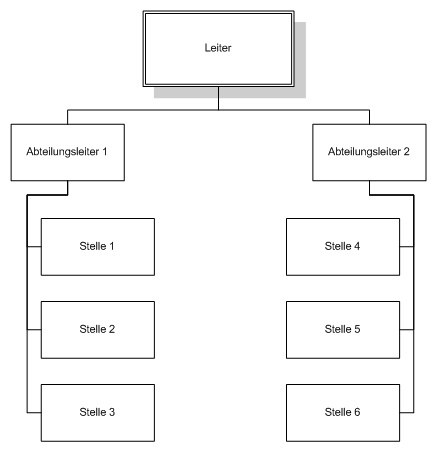
\includegraphics[keepaspectratio]{images/figure42.jpg}} \hfill{}

\caption{Abb. 4.2: Beispiel für ein Einlinienorganisation (Bernd Bosch,
CC BY-SA 3.0), Quelle:
\url{https://commons.wikimedia.org/wiki/File:Einliniensystem.jpg} (CC
Public Domain)}

\end{figure}%

\subsubsection{Mehrlinienorganisation}\label{mehrlinienorganisation}

Diese unterscheidet sich von der Einlinienorganisation dadurch, dass es
hier mehrere Kommunikationswege und Verbindungen zwischen den einzelnen
Organisationseinheiten gibt. In dem Beispiel von Thommen (2000) werden
drei Hierarchien bzw. Organisationsebenen dargestellt (vgl.
\hyperref[figure43]{Abb. 4.3}).

\begin{figure}

\pandocbounded{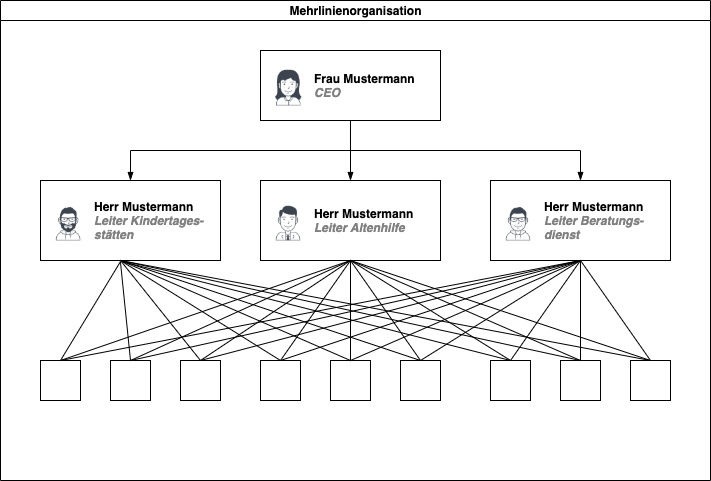
\includegraphics[keepaspectratio]{images/figure43.png}} \hfill{}

\caption{Abb. 4.3: Mehrlinienorganisation (eigene Darstellung, nach
Thommen, 2000, S. 696))}

\end{figure}%

Auf der ersten Ebene ganz oben befindet sich die Unternehmensleitung,
dann gibt es eine zweite Ebene, die Abteilungen und auf der dritten
Ebene existieren die Sachbereiche bzw. die einzelnen Teileinheiten oder
vielleicht die einzelnen Häuser bei größeren sozialen Trägern. Die erste
und zweite Ebene hat eine gewisse Ähnlichkeit mit der
Einlinienorganisation. Aber es kommt noch etwas Neues hinzu, nämlich,
dass zwischen zweiter und dritter Ebene, wo letztlich alle Geschäfts-
und Managementprozesse umgesetzt werden müssen, Mehrfachzugehörigkeiten
existieren oder einfach mehrere Ansprechpartner zur Verfügung stehen.
Wenn auf der untersten, dritten Ebene z. B. Wohngruppen angesiedelt
sind, dann können die Mitarbeitenden in den Wohngruppen jeweils
gleichzeitig alle Personen auf der zweiten Ebene wie z. B. aus der
Personalabteilung, der Controllingabteilung oder möglicherweise aus dem
Einkauf und der Beschaffung ansprechen. Es gibt immer die Möglichkeit,
dass mehrere Personen für bestimmte Fragestellungen angesprochen werden
können. Ein Vorteil ist hier, dass es kurze Wege gibt und immer die
fachlichen Expert*innen angesprochen werden können und dann entsprechend
Probleme im direkten Austausch besprochen werden können, ohne eine
komplizierte Hierarchie einhalten zu müssen. Ein Nachteil ist, dass
aufgrund der Vielzahl an Kommunikationswegen oder -möglichkeiten sich
eine Organisation schnell zu einem nicht mehr überblickbaren Geschehen
entwickelt und dass die Einrichtungsleitung ggf. häufiger mit Problem-
und Konfliktfällen zu tun hat.

\subsubsection{Stabslinienorganisation}\label{stabslinienorganisation}

Dabei handelt es sich im engeren Sinne um eine Einlinienorganisation,
die um ein weiteres Element ergänzt worden ist, die Stabsstellen.
Stabsstellen sind solche Aufgaben- oder Funktionsbereiche innerhalb der
Einrichtung, die eine spezielle Aufgabe zur Entlastung des Vorstandes
und natürlich auch zur Verbesserung des organisationsbezogenen
Managements ausfüllen.

\begin{figure}

\pandocbounded{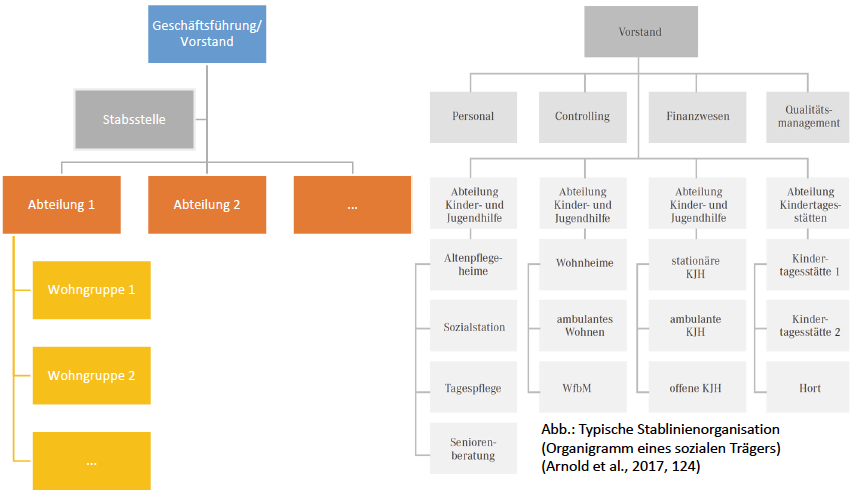
\includegraphics[keepaspectratio]{images/figure44.png}} \hfill{}

\caption{Abb. 4.4: Typische Stablinienorganisation anhand eines
Organigramm eines sozialen Trägers (nach Liedke, 2017, S. 124)}

\end{figure}%

In der \hyperref[figure44]{Abb. 4.4} sind beispielsweise Stabsstellen
für Personal- und Finanzwesen sowie für das Controlling und
Qualitätsmanagement zu sehen. Und darüber hinaus lassen sich natürlich
noch weitere Stabsstellen denken. Die dargestellte Einrichtung ist so
gegliedert, dass neben dem Vorstand bzw. der Geschäftsführung und den
Stabsstellen eine klassische Einlinienorganisation mit den einzelnen
Abteilungen existiert. In dem Beispiel gibt es vier Abteilungen, die
entweder Kinder- und Jugendhilfereferate oder allgemein den Bereich
Kindertagesstätten verwalten. Darüber hinaus sind verschiedene
Teilbereiche der Referate zu sehen, die nach dem jeweiligen Sachgebiet
angegliedert sind. Ein Vorteil dieser Organisationsstruktur ist, dass
die Stabsstellen genau dazu geeignet sind, den Vorstand und
Geschäftsführung zu entlasten und dass ihr Spezial- und Expertenwissen
die professionelle Arbeit der Einrichtung entsprechend zur Verfügung
steht. Nachteil dieses Organigramms könnte sein, dass sich die
Einrichtung möglicherweise sog. graue Eminenzen entwickelt, dass die
Stabsstellen über gewisses Wissen verfügen und von den einzelnen
Teilabteilungen genutzt werden kann, z. B. indem man direkt die
Controllingabteilung anfragt und der Vorstand bei bestimmten Fragen
nicht miteinbezogen wird, obwohl dies notwendig ist. So könnten sich die
Stabsstellen ihrer Kompetenz überheben, weil diese in der Regel keine
eigene Entscheidungsbefugnis besitzen, sondern „Handlungsgehilfen'' der
Unternehmensleitung darstellen.

\subsubsection{Matrixorganisation}\label{matrixorganisation}

Wie der Name vermuten lässt, geht es bei Matrixorganisationen um ein
Geflecht verschiedener Bereiche und Abteilungen innerhalb der
Organisation.

\begin{figure}

\pandocbounded{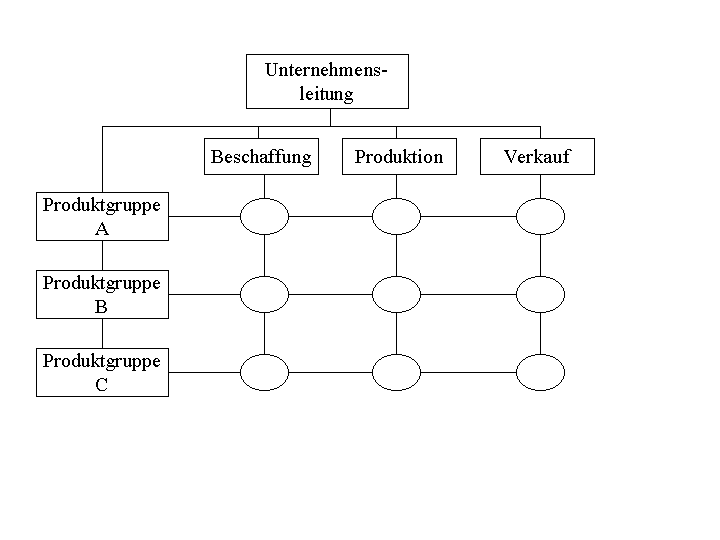
\includegraphics[keepaspectratio]{images/figure45.png}} \hfill{}

\caption{Abb. 4.5: Matrixorganisation (Wagner, 2004, \emph{Skizze einer
Matrixorganisation},
\url{https://upload.wikimedia.org/wikipedia/de/c/cb/Matrixorganisation.png}
(Public Domain))}

\end{figure}%

Die \hyperref[figure45]{Abb. 4.5} zeigt ein Unternehmen aus dem
produzierenden Gewerbe, wo verschiedene Produkte hergestellt werden. In
dem Unternehmen gibt es verschiedene Produkte, für die Manager zuständig
sind und verschiedene Verantwortliche für z. B. Einkauf, Produktion,
Verkauf (= Input-Output-Prozess). Die einzelnen Bereiche sind hier nicht
nach Funktionsbereichen untergliedert, wie dies bei den Einlinien-,
Mehrlinien- oder Stabslinienorganisation üblich ist, sondern nach dem im
jeweiligen Teilprozessverantwortlichen und Herstellungsstufen.
Anfänglich müssen Material und Bauteile beschafft werden, wobei die
Produktgruppe A beispielsweise mit der Beschaffungsabteilung den
Materialeinkauf organisiert. Wenn es dann dazu übergeht, dass das
Produkt hergestellt werden muss, ist der Produktionsmanager
Ansprechpartner. Wenn das Produkt verkauft werden soll, wird schließlich
die Marketingabteilung tätig.

Ein klarer Vorteil dieser Organisationsstruktur ist, dass die einzelnen
Bereiche sich jeweils direkt miteinander verständen können und dass
nicht noch einmal eine übergeordnete Einheit eingeschaltet werden muss.
Es steht keine Entscheidungsinstanz dazwischen; dadurch geht die
Entscheidungsfindung und auch die Umsetzung um ein Vielfaches. Ein
Nachteil ist beispielsweise, dass es hier möglicherweise auch manchmal
zu Kompetenzgerangel kommen könnte, wenn möglicherweise etwas im
Beschaffungsbereich entschieden wurde, was für den Produktionsbereich
suboptimal war und dazu geführt hat, dass ein Teil der Produktion auf
dem Schrott gelandet ist.

Die Matrixorganisation kann auch auf soziale Einrichtungen übertragen
werden. Bei den Produktgruppen könnten die verschiedenen
Leistungsbereiche oder, wenn man es als Produktgruppe übersetzt, die
Wohngruppen A, B und C stehen. Dann gibt es innerhalb der Organisation
auch noch verschiedene andere Ansprechpartner, die Leitung, die
Fachberatung oder aus anderen Bereichen wie z. B. Finanzen, Wirtschaft,
Controlling. Letztgenannte Verantwortliche können jeweils von den
einzelnen Wohngruppen direkt angesprochen werden.

\subsubsection{Produktgruppenorganisation}\label{produktgruppenorganisation}

Diese Organisationsstruktur stellt eine Kombination aus der Einlinien-
und Stabslinienorganisation dar (vgl. \hyperref[figure46]{Abb. 4.6}).

\begin{figure}

\pandocbounded{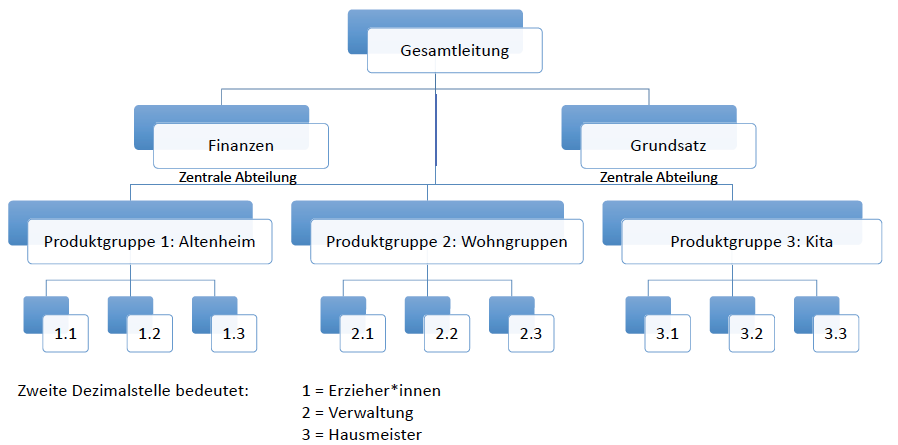
\includegraphics[keepaspectratio]{images/figure46.png}} \hfill{}

\caption{Abb. 4.6: Produktgruppen-Organisation mit zentralen Abteilungen
(nach Müller-Schöll \& Priepke, 1992, S. 87) zit . n. (Wöhrle, 2012, S.
34))}

\end{figure}%

Es gibt auf oberster Ebene die Geschäftsleitung, die verantwortlich ist
für die verschiedenen zentralen Bereiche, nämlich die Bereiche für die
Produktgruppe 1, 2, 3 usw. Die Bereichsleitung wird wiederum unterstützt
durch die Referate Finanzen und Grundsatz, um bestimmte Aufgaben zentral
abzusprechen sowie die Leitung zu unterstützen und zu entlasten. Darüber
hinaus gibt es auf der zweiten Ebene die einzelnen Produktgruppen, d.~h.
also innerhalb eines Altenheimes, Wohngruppe oder Kita gibt es
unterschiedliche (teilautonome) Teilbereiche bzw. Verantwortliche, z. B.
Heimverwaltung, angestellte Erzieher*innen und Hausmeisterdienst. Ein
Vorteil dieser Struktur ist, dass sehr stark klientenorientiert
gearbeitet werden kann. D. h. für ein Altenheim oder eine Kita gibt es
genau einen Leistungserbringer, der exakt diese Leistung und die soziale
Dienstleistung anbietet. Nachteil könnte möglicherweise sein, dass hier
die Wechselbeziehungen, nämlich das Lernen zwischen Einrichtungen eines
Trägers nicht so einfach möglich ist. Das Wissen über organisationale
Abläufe im Altenheim, in den Wohngruppen und in der Kita kann
schließlich auch zur Verbesserung der professionellen Arbeit
ausgetauscht werden.

Bisher haben wir uns mit der Aufbaustruktur beschäftigt, wobei es um die
Frage ging, wie innerhalb von Organisationen die Struktur bzw. der
formale Aufbau in Form von Organigrammen stattfinden kann.

\subsubsection{Reflexionsaufgabe}\label{reflexionsaufgabe}

In diesem Abschnitt ging es um die Struktur- und die Prozessperspektive
im organisationsbezogenen Management, also um die Aufbau- und
Ablaufstruktur. Die folgende Reflexionsaufgabe beschäftigt sich mit den
verschiedenen Organigrammen. Diskutieren Sie dabei die folgenden drei
Fragen:

\begin{enumerate}
\def\labelenumi{\arabic{enumi}.}
\item
  Welche Charakteristika fallen Ihnen in den einzelnen Modellen noch
  auf, die vielleicht bisher nicht erwähnt wurden?
\item
  Sehen Sie noch weitere Vor- und Nachteile, die für oder gegen diese
  Organisationsformen sprechen?
\item
  Wie meinen Sie, lassen sich die Strukturentwürfe in den sozialen
  Einrichtungen nutzen und umsetzen?
\end{enumerate}

Bisher haben wir uns mit der Aufbaustruktur beschäftigt, wobei es um die
Frage ging, wie innerhalb von Organisationen die Struktur bzw. der
formale Aufbau in Form von Organigrammen stattfinden kann.

\section{Prozessperspektive}\label{prozessperspektive}

\subsection{Phasen des
Prozessmanagements}\label{phasen-des-prozessmanagements}

Im Folgenden gehen wir zur prozessbezogenen Perspektive über. Dabei
steht die Ablauforganisation im Mittelpunkt und es stellt sich die
Frage, wie bestimmte Aufgaben innerhalb der Einrichtung strukturiert und
ggf. auch durch Verbesserungen optimiert werden können. Wir beginnen
diesen Teil jetzt mit einem Phasenmodell von Schiersmann \& Thiel
(2014), die den vollständigen Ablauf des Prozessmanagements in sieben
Phasen untergliedern (vgl. \hyperref[figure47]{Abb. 4.7}).

\begin{figure}

\pandocbounded{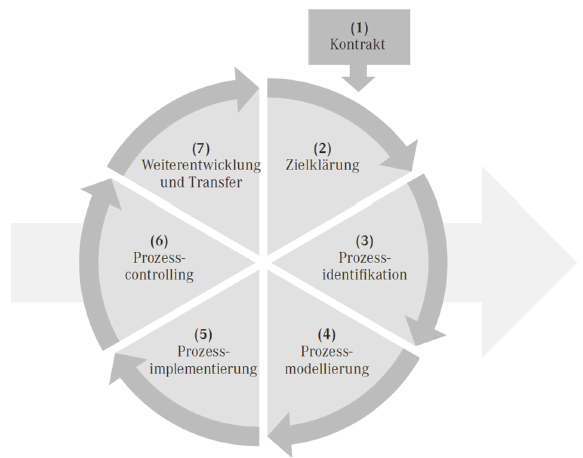
\includegraphics[keepaspectratio]{images/figure47.png}} \hfill{}

\caption{Abb. 4.7: Phasen des Prozessmanagements (nach Schiersmann \&
Thiel, 2014, S. 348-350)}

\end{figure}%

In der ersten Phase geht es um das Contracting, d.~h. der Kontrakt bzw.
Auftrag muss besprochen und festgelegt werden. Es muss definiert werden,
wer wie verantwortlich ist, dass ein Prozess überhaupt erst einmal
erstellt und entwickelt werden kann. Der Zeitrahmen muss definiert
werden und natürlich auch das anvisierte Ziel. In der zweiten Phase muss
festgelegt werden, wie der Prozess zukünftig gestaltet sein soll bzw.
was das Ergebnis sein soll. Im dritten Schritt müssen der Prozess bzw.
dessen Einzelbestandteile, Teilaufgaben und verantwortliche Personen
identifiziert werden. Und schließlich geht es viertens darum, den
Prozess zu modellieren. Mithilfe einer Visualisierung wird sich ein
Überblick darüber verschafft, wie die einzelnen Prozessschritte, die
Abläufe und Aufgaben sinnvoll arrangiert und verändert werden können.
Die Phase fünf setzt dann gewissermaßen diesen neu gefundenen und
entwickelten Prozess zusammen und es erfolgen Tests. In der sechsten
Phase erfolgt das Prozesscontrolling, z. B. indem das
Qualitätsmanagement die neuen Prozesse prüft, dafür Vorlagen entwickelt
und entsprechend dokumentiert. Der gesamte Prozess ist als
Controllingprozess zu verstehen. Schließlich in der siebten Phase sollen
nach diesem Modell eine Weiterentwicklung und ein Transfer angestrebt
werden, d.~h. ein Prozess ist definiert aber mit hoher
Wahrscheinlichkeit wird sich immer etwas herausstellen, was zukünftig
noch verbessert und anders umgesetzt werden kann. Daraus folgt, dass
sich um eine ständige Optimierung der Prozesse gekümmert werden muss.
Dieses 7-Phasen-Modell von Schiersmann und Thiel Schiersmann \& Thiel
(2014) versucht darzustellen, wie innerhalb der Einrichtung Prozesse
gemanagt und umgesetzt werden können.

\subsection{Aufgabenfolgeplan bzw. Flussdiagramm
(Flowcharts)}\label{aufgabenfolgeplan-bzw-flussdiagramm-flowcharts}

Im Folgenden sollen zwei Instrumente für das Prozessmanagement innerhalb
von Einrichtungen dargestellt werden. Im Aufgabenfolgeplan bzw.
Flussdiagramm erfolgt erstens eine Visualisierung von Prozessen. Dafür
gibt es eine eigene Zeichensprache, z. B. ovale Kreise für Start- und
Endereignisse, Kästchen für Aufgabenstellungen, Pfeile für
Kommunikationswege, Rauten für Entscheidungssituationen usw. (vgl.
\hyperref[figure48]{Abb. 4.8}).

\begin{figure}

\pandocbounded{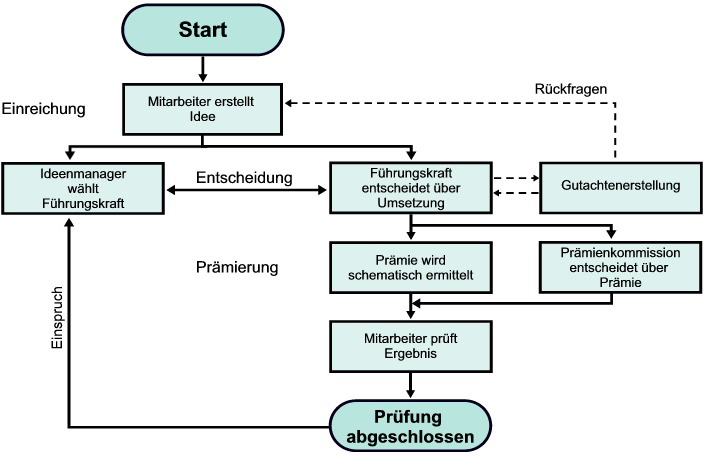
\includegraphics[keepaspectratio]{images/figure48.jpg}} \hfill{}

\caption{Abb. 4.8: Flowchart Ideenprämierung (Hagenmaier, CC-BY-SA 3.0)}

\end{figure}%

Anfangs wird eine Idee von Mitarbeitenden eingereicht, dann ist ein
Entscheidungsprozess in dem Gremium anzuregen, der zwischen Ideenmanager
und Führungskräften zu organisieren ist. Danach ist zu entscheiden, ob
eine Idee umgesetzt werden soll. Für die Entscheidung über die Umsetzung
müssen gegebenenfalls noch Gutachten von extern eingeholt werden. Falls
die vom Mitarbeiter vorgeschlagene Idee sinnvoll erscheint und umgesetzt
werden kann, kommt es zur Prämierung dieser Idee. Es gibt eine
Prämienkommission, die darüber entscheidet und diese legt dann dem
Mitarbeiter die Entscheidung über die Höhe der Prämie vor, welcher sie
im besten Fall akzeptiert. Diese Übersicht hilft dabei, den Prozess
darzustellen, wobei es allgemein gesprochen darum geht, dass eine Idee
entwickelt und prämiert wird. Ein Flussdiagramm versucht den Weg der
Entscheidungen und die Verantwortlichen, die einzubeziehen sind, zu
definieren. Es sind keine konkreten Zeitangaben gemacht worden, was ggf.
erweiterungsfähig ist.

\subsection{Prozesslandkarte}\label{prozesslandkarte}

Dieses zweite Instrument für das Prozessmanagement bildet, wie der Name
vermuten lässt, Prozesse in Form eines Überblicksplans, in dem die
verschiedenen Aufgaben, Verantwortlichkeiten und Schritte detailliert
dargestellt sind, ab.

\begin{figure}

\pandocbounded{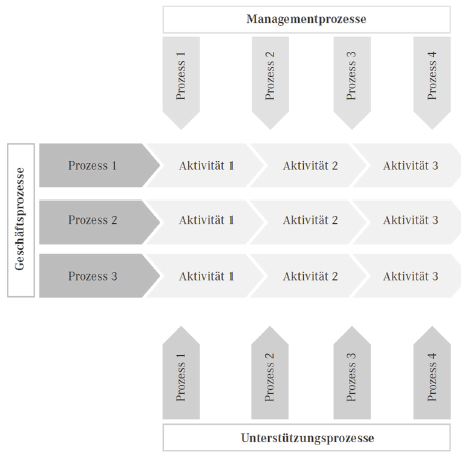
\includegraphics[keepaspectratio]{images/figure49.png}} \hfill{}

\caption{Abb. 4.9: Schema einer Prozesslandkarte (nach Liedke, 2017, S.
155)}

\end{figure}%

In dem in \hyperref[figure49]{Abb. 4.9} dargestellten Beispiel gibt es
drei Bereiche, die miteinander prozessual vernetzt sind und sich
gegenseitig beeinflussen. Es können dabei drei Prozessebenen, wie z. B.
Management-, Geschäfts- und Unterstützungsprozesse unterschieden werden,
wie dies weiter oben schon anhand des St.~Galler Management-Modells
dargestellt worden ist. Zu Managementprozessen gehören z. B.
Leitungsaufgaben. Unter Geschäftsprozessen können alle Alltagsprozesse
zusammengefasst werden und bei Unterstützungsprozessen geht es darum,
dass Unterstützungsmaßnahmen wie z. B. Einkauf, Reinigung,
Hausmeisterdienste organisiert werden. In der Mitte des Schemas kann man
die einzelnen Geschäftsprozesse erkennen, die jeweils im Überblick
dargestellt werden und die einzelnen Teilaktivitäten beinhalten. Die
Teilaktivitäten werden jeweils unterstützt durch die unten dargestellten
Unterstützungsprozesse sowie durch die Managementprozesse wie z. B.
Personal, Controlling und Qualitätsmanagement.

\begin{figure}

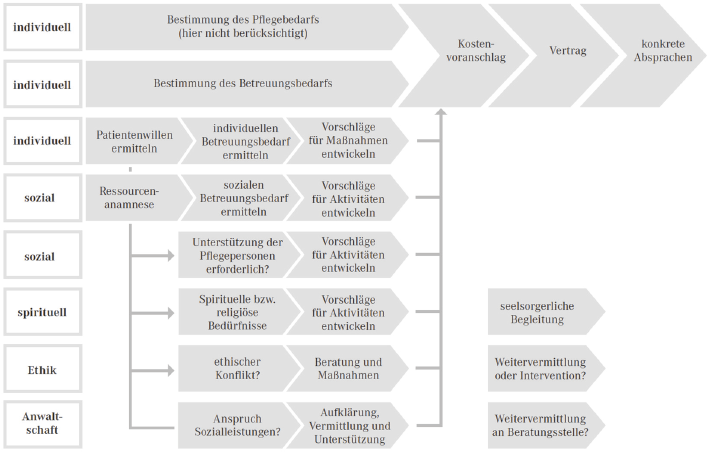
\includegraphics[width=0.8\linewidth,height=\textheight,keepaspectratio]{images/figure410.png} \hfill{}

\caption{Abb. 4.10: Prozesslandkarte Erstgespräch zur Bestimmung des
Betreuungsbedarfs in ambul. Altenhilfe (nach Liedke, 2017, S. 157)}

\end{figure}%

In \hyperref[figure410]{Abb. 4.10} wird ein relativ komplexer Prozess,
nämlich der für das Erstgespräch zur Bestimmung des Betreuungsbedarfs in
der ambulanten Altenhilfe dargestellt. Das Beispiel ist entstanden im
Rahmen eines zurückliegenden Projekts zur Analyse diakonischer Träger in
Sachsen. In den Gesprächen, die geführt wurden, ist genau dieses Modell
aufgefallen. Dies wurde validiert und durch die jeweilige Einrichtung
abgesichert. Auf der linken Seite sind die verschiedenen Prozessebenen
dargestellt. Es gibt drei Prozessbereiche, die auf der individuellen
Entscheidungsebene relevant sind: Es gibt die soziale Ebene, wo es um
Fragen wie das Zusammenwirken mit Angehörigen oder dem Pflegepersonal
geht. Dann gibt es eine spirituelle Ebene, wo es um die Berücksichtigung
religiöser Bedürfnisse geht, und die ethische Ebene, was relevant ist
für die Qualitätssicherung und den Umgang mit Konflikten innerhalb von
Prozessen. Außerdem wird auf Ebene der Anwaltschaftlichkeit dargestellt,
was die Sozialarbeitenden bzw. die Soziale Arbeit allgemein für eine
Verantwortung trägt sowie wie und mit welchem Anspruch sie gewisse
soziale Dienstleistungen anbietet.

Grau hinterlegt sind die Teilprozesse, die der Bestimmung des Pflege-
und Betreuungsbedarfs dienen, um einen Kostenvoranschlag zu erstellen.
Auf Basis dessen kann dann der Vertrag ausgefertigt werden und es kann
zu einer konkreten vertraglichen Absprache kommen. Auf der individuellen
Ebene müssen noch weiterhin der Patientenwille bzw. der individuelle
Betreuungsbedarf beachtet und erfasst werden. Auf der sozialen Ebene
geht es darum, die verschiedenen Ressourcen, die noch für den
Betreuungsprozess zur Verfügung stehen, richtig zu koordinieren. Darüber
hinaus gilt es noch, weitere Unterstützungsmaßnahmen oder die
Unterstützung der Pflegepersonen einzuplanen, z. B. wie religiöse
Bedürfnisse durch seelsorgerliche Begleitung unterstützt werden und
ethische Konflikte gelöst werden können. Sollte eine Betreuung oder
Beratungsmaßnahmen außerhalb der Einrichtung notwendig sein, kann
entsprechend weiterverwiesen werden (z. B. Therapien, Demenzbehandlung).
Auf einer anderen individuellen Ebene geht es schließlich darum, dass
ein zusätzlicher Bedarf an Pflege festgestellt wurde, welcher zu einem
höheren Maß an benötigten Sozialleistungen führt. Wurde im Erstgespräch
nicht festgestellt, dass diese zusätzlichen Leistungen benötigt werden,
so müsste das später erneut überprüft werden.

\section{Organisationskultur}\label{organisationskultur}

\subsection{Was ist Kultur?}\label{was-ist-kultur}

Als Kultur kann man ganz allgemein ein gemeinsames geteiltes und
gelebtes Handlungs-, Orientierungs- und Symbolsystem verstehen. Damit
ist gemeint, dass es mehrere Personen gibt, die gemeinsam bestimmte
Werte, Überzeugungen und auch gewisse Handlungsweisen sowie
ritualisierte Praktiken teilen und als wichtig erachten. Darüber hinaus
verfügen Kulturen immer über bewusste und sichtbare bzw. unbewusste und
unsichtbare Elemente. Diese Unterscheidung wurde in die
Organisationskulturdebatte von Edgar Schein eingeführt und geht
letztendlich auf die Psychoanalyse zurück. Allgemein kann Kultur als
handlungsleitend verstanden werden: auf der einen Seite, sind wir durch
Kultur (z. B. Werte, Überzeugungen und Normen) geprägt, auf der anderen
Seite prägen wir auch die Kulturen, in denen wir leben. Kultur wird
nicht bewusst erlernt, sondern in einem meist längerfristigen
Sozialisationsprozess erworben bzw. angeeignet. Ein sehr bekanntes
Modell ist beispielsweise die Metapher des Eisbergs (nach Edgar Schein).
Es gibt relativ wenig Fläche bzw. Volumen eines Eisbergs oberhalb der
Wasseroberfläche. Dort sind die sichtbaren bzw. bewusst wahrnehmbaren
Aspekte von Kultur angesiedelt wie z. B. Arbeitsklima, Literatur,
Bräuche, Tänze und auch Architektur. All das stellen die wahrnehmbaren
und sichtbaren Elemente von Kultur dar. Die Sprache könnte man an der
Wasseroberfläche ansiedeln. Sprache ist für die Kommunikation und
Orientierung in der sichtbaren Welt von besonderer Bedeutung, aber auf
der anderen Seite gibt es auch unbewusste Anteile oder weniger bewusster
Anteile wie z. B. die Grammatik oder die verschiedenen Bedeutungen von
Wörtern und Sinnzusammenhängen, die man erst dann richtig verstehen
kann, wenn man sich ein Mindestmaß einer Sprache bzw. Sprachkultur
angeeignet hat. Und im unteren Bereich des Eisbergs befinden sich die
unbewussten Gedanken und Handlungskonzepte, wie z. B.
Wahrnehmungsmuster, Umgang mit Hierarchien, Machtverhältnisse,
Vorstellungen von Logik, Schönheit, Wahrheit, Erziehungsideale etc. Alle
vorgenannten Aspekte gehören zum unbewussten Teil des Eisbergs.

\subsection{Was ist eine
Organisationskultur?}\label{was-ist-eine-organisationskultur}

Nicht nur Individuen können Mitglieder einer Kultur sein, sondern auch
Organisationen können selbst eigene Kulturen ausbilden.
Organisationskulturen haben nach Schreyögg \& Geiger (2016) in der Regel
impliziten Charakter, sie sind nicht ohne Weiteres greif- und fassbar,
sondern sie existieren im Hintergrund, sind unbewusst, nicht explizit
niedergeschrieben bzw. verschriftlicht:

Organisationkultur(en) \ldots{}

\begin{itemize}
\item
  ist ein im Wesentlichen \emph{implizites} Phänomen;
\item
  werden im Unternehmensalltag \emph{praktiziert}, gelebt und sind
  selbständig;
\item
  beziehen sich auf \emph{gemeinsame} Orientierungen, Werte etc.
  (kollektives Phänomen);
\item
  ist das Ergebnis eines \emph{Lernprozesses} im Umgang mit Problemen
  aus der Umwelt und der internen Koordination;
\item
  repräsentiert die ‚\emph{konzeptionelle Welt}' bzw. `\emph{Weltbild}'
  ihrer Mitglieder und vermittelt Sinn und Orientierung in einer
  komplexer Welt;
\item
  wird in einem \emph{Sozialisationsprozess} vermittelt und nicht
  bewusst erlernt. (Schreyögg \& Geiger, 2016, pp. 177--178)
\end{itemize}

Auch wenn wir in Leitbildern versuchen, Werte, Überzeugungen und
Visionen, die Geschichte der Einrichtung niederzuschreiben, ist stets
keine vollständige Organisationsbeschreibung möglich.
Organisationskulturen entwickeln sich gewissermaßen selbstständig und
können nicht begrenzt werden durch eine Ansage der Geschäftsführung,
sondern entwickeln sich sozusagen parallel zum oder im Rahmen des
Alltags. Organisationskulturen beziehen sich auf gemeinsame
Orientierung, Werte und Überzeugungen und sind damit ein kollektives
Phänomen. So wie bereits beschrieben, geht es um das Vorhandensein
gemeinsam geteilter Werte, Überzeugungen und Symboliken. Beispielsweise
äußert sich das in der Berufskleidung, Leitbildbeschreibung und
Kommunikationsweise. Organisationskulturen sind schließlich Ergebnis
eines Lernprozesses im Umgang mit der externen und internen Umwelt; sie
sind dynamisch, entwickelt und verändern sich über den Zeitverlauf. Sie
müssen sich letztendlich immer mit der internen und externen Umwelt
auseinandersetzen. Die externe Umwelt veranlasst z. B. aufgrund von
gesetzlichen Rahmenbedingungen oder bei Veränderungen der Bedarf von
Zielgruppe Veränderungen innerhalb der Einrichtung (z. B.
Dokumentationspflicht). Konflikte, Probleme oder der Umgang mit
komplexen Herausforderungen bedingt häufig auch eine Thematisierung und
Entwicklung der Kultur innerhalb von Organisationen (z. B.
Konfliktregulierung, Aufstellen von Kommunikationsregeln). Alle
vorgenannten Aspekte können schließlich Auslöser von organisationalen
Lernprozessen sein. Schließlich repräsentiert die Organisationskultur so
etwas wie eine konzeptionelle Welt der Organisationsmitglieder, d.~h.
Organisationen wurden und werden dafür geschaffen, dass sie gemeinsame
Ziele zu verwirklichen helfen. Die Organisationskultur ist gewissermaßen
das Skript, was man im Kopf hat, wie man in der Einrichtung
zusammenarbeiten kann. Dementsprechend werden Sinn und Orientierung
innerhalb von Organisationen vermittelt und die Organisationskultur
hilft dabei, komplexe Realitäten zu bewältigen. Bestimmte
Handlungsweisen, Umgangsformen oder auch Kommunikationsregeln sind
letztlich dafür verantwortlich, dass das Miteinander bzw. die
Zusammenarbeit gelingen kann. Organisationskulturen können weder
vollständig explizit gemacht noch vollständig erlernt werden (wie z. B.
ein QM-Handbuch). Sie werden im Rahmen eines Sozialisationsprozesses
regelmäßig reflektiert und angeeignet.

\subsection{Modell der Organisationskultur nach Edgar
Schein}\label{modell-der-organisationskultur-nach-edgar-schein}

Im nächsten Schritt wird auf ein Modell von Edgar Schein
zurückgegriffen, der sich auf verschiedenen Kulturebenen die Frage
gestellt hat, wie Organisationskulturen aufgebaut sind. Dabei werden
drei Ebenen unterschieden, die von den sichtbaren über teilweise
sichtbare hin zu unsichtbaren Aspekten von Kulturen reichen. Auf der
sichtbaren Ebene sind die Artefakte angesiedelt, welche die
objektivierte Organisationskultur darstellen. Auf der zweiten Ebene gibt
es teilweise sichtbaren bzw. teils unbewusste Teile von
Organisationskultur, d.~h. die bekundeten Werte, die zwar
niedergeschriebene Werte und Überzeugungen darstellen. Auf der dritten
Ebene sind die unsichtbaren, meist unbewussten Anteile von
Organisationskultur, die sogenannten Grundannahmen, angesiedelt.
Dahinter verbirgt sich, wie leicht zu erkennen ist, das Konzept des
Eisbergs: die Artefakte sind direkt an der Wasseroberfläche und
sichtbar, die bekundeten Werte sind das Eisschelf, das noch ca. zwei bis
drei Meter ins Wasser sichtbar ist. Die Grundprämisse ist der Teil des
Eisbergs, der unterhalb der Wasseroberfläche ist.

Die Artefakte sind die sichtbaren Teile von Organisationen, z. B.
Strukturen und Prozesse, die nachvollziehbar, beobachtbar und aber ggf.
schwierig zu entschlüsseln sind. Dazu gehört bspw. die Sprache, die wir
verwenden. Wir setzen Sprache ein, kennen Rituale, die bestimmte
Bedeutungen haben, z. B. Tagesabläufe, Kleidung, Umgangsformen,
Kommunikationsregeln, die Fachsprache, Anreden Du oder Sie. Bei den
bekundeten Werten, auf der teilweise sichtbaren Ebene, handelt es sich
um die Strategien, Ziele und Visionen der Einrichtung, die offenkundig
und teilweise verschriftlicht sind, z. B. in Form von Leitbild,
Führungskonzeptionen oder ganz allgemein die Konzeption der Einrichtung.
Darin werden Prinzipien dargestellt, wie zusammengearbeitet werden kann
und auf welcher Basis eine professionelle Haltung existiert. Zu den
Grundannahmen gehören grundlegende Prämissen der Einrichtung, die weder
bewusst, sichtbar noch niedergeschrieben sind, z. B. das Bild vom Kind,
Weltbilder, Überzeugungen von Humanität. Dazu gehören u. a. Anschauungen
und Wahrnehmungen, Gedanken und Gefühle, die in der Einrichtung von
Bedeutung sind. Außerdem können wir uns Fragen stellen wie z. B.: Wie
pflegen wir die Beziehungen nach außen zu unserer Umwelt? Wie gehen wir
mit den Klient*innen um? Welche nicht impliziten Handlungsüberzeugungen
gibt es? Welche Überzeugung von Transparenz, Offenheit leben wir?

\subsection{Strategien des
Kulturwandels}\label{strategien-des-kulturwandels}

Im Folgenden werden verschiedene Strategien für den Kulturwandel
vorgestellt. Mit Kulturwandel ist gemeint, dass Organisationskulturen
nicht feststehen, sondern dass sie sich in einem kontinuierlichen
Veränderungsprozess befinden. Im vorgestellten Modell von Bate (2010;
zit n. Wöhrle, 2001, S. 43-5) werden vier dieser Strategien
unterschieden, die aggressive, die partizipatorische, die korrosive und
die doktrinäre Strategie.

Bei der \emph{aggressiven} Strategie geht es darum, dass durch eine
entsprechende Anweisung durch die Geschäftsführung eine
Organisationskulturentwicklung ausgelöst wird. Es wird mit anderen
Worten das neue Handeln angeordnet, aufgezwungen und relativ schnell,
das ist der Vorteil, einen gewissen Impuls setzen bzw. Veränderungen
bewirken. Auf der anderen Seite, das wäre ein Nachteil, könnte daraus
auch eine Lagerbildung bzw. Pluralisierung in der Mitarbeiterschaft
erwachsen.

Auf der \emph{partizipatorischen} Ebene wird mithilfe von Team- und
Gruppenarbeit versucht, gemeinsame Ansätze zu entwickeln. Das ist
grundsätzlich der kooperative Ansatz und hier wird mehr oder weniger
danach gesucht, einen gemeinsamen Weg zu finden. Alle werden
gewissermaßen an der Problemlösung beteiligt. Vorteil davon ist, es gibt
Zusammenarbeit, Mitsprache und Teilhabe an der Entscheidungsfindung bzw.
an der Umsetzung. Ein Nachteil könnte dabei sein, dass es hier zu einem
Wandel zweiter Ordnung (siehe Organisationsentwicklung in Abschnitt 6)
kommen kann. Damit ist gemeint, dass Veränderungsprozesse als sehr
gravierend empfunden werden und es zu Brüchen kommen kann. Die
Kulturveränderung ist so tiefgreifend, dass eine komplett neue
Organisationsvision, eine neue Strategie oder/und neue Struktur für die
Einrichtung gefunden werden muss. Andererseits kann es aber auch um eine
Optimierung verschiedener (Teil-)Aufgaben, Prozesse und Strukturen
gehen.

Bei der \emph{korrosiven} Strategie wir die „politische'' Perspektive
innerhalb von Organisationen betont. Dabei wird versucht, Koalitionen zu
schmieden bzw. Netzwerke aufzubauen. Damit ist die Eröffnung von
informellen Wegen jenseits bekannter Strukturen, Verantwortlichkeiten
und Entscheidungsprozesse gemeint. Ein Vorteil ist, dass Ideen aus der
„zweiten Reihe'' ebenso kulturprägend sein können. Grundsätzlich gibt es
auch in der Sozialen Arbeit (im Sinne des Empowerments) das Prinzip,
Klient*innen stets an der Lösungsfindung zu beteiligen. Ein Nachteil
kann sein, dass es natürlich keinen Königsweg geben kann. Es könnten
sich ggf. Strukturen und Konstellationen ergeben, die zu einer
Lagerbildung und Spaltung führen und auch positive Entwicklungen
beeinträchtigen oder verhindern können.

Bei der \emph{indoktrinären} Strategie geht schließlich darum, dass man
auch auf dem Wege der Aus-, Weiter- und Fortbildung Organisationskultur
verändern kann. Vorteilhaft ist hierbei, dass relativ schnell durch eine
Wissensvermittlung eine Umorientierung stattfinden kann. Ein Nachteil
könnte sein, mit ``Umerziehungsprogrammen'' nicht immer ein
Veränderungsprozess bewirkt werden kann, da Organisationskulturen mehr
oder weniger implizit sind und diese nicht „auswendig'' gelernt werden
können.

Kurz zusammengefasst: Veränderungen können bewirkt werden durch eine
Machtausübung, wie z. B. durch Dienstanweisungen. Auf der
partizipatorischen Ebene geht es darum, Beteiligung und Teilhabe zu
ermöglichen. Auf der Ebene der informellen Netzwerke können z. B. durch
Flurfunk, Kaffeeecken oder Raucherinseln durchaus kommunikative Touch
Points beschaffen werden, wo man sich ungezwungen über neue Ideen
austauschen kann. Außerdem sind auch gezielte Weiterbildungen bzw.
Wissensvertiefungen hilfreich, wie z. B. Kennlernseminare,
Kickoff-Veranstaltung für neue Mitarbeitende, in denen Grundprinzipien,
Arbeitsweisen und die Funktionsweise der Einrichtung sowie
verantwortliche Personen innerhalb der Einrichtung vorgestellt werden.
Die vier darstellten Strategie sind nicht getrennt zu betrachten,
sondern ergänzen sich gegenseitig. Es kann auch so verstanden werden,
dass hier je nach Situation eine unterschiedliche Herangehensweise
gewählt und umgesetzt werden kann.

\subsection{Integrated Culture Framework nach Groysberg, Lee, Price und
Cheng
(2018)}\label{integrated-culture-framework-nach-groysberg-lee-price-und-cheng-2018}

Im Rahmen einer vor einigen Jahren erschienen empirischen Studie von
Groysberg et al. (2018a; dt. Groysberg et al., 2018b) wurde der Frage
nachgegangen, welche Bedeutung Organisationskulturen für den Erfolg von
Unternehmen haben können. Die Untersuchung beinhaltete eine Analyse der
Organisationskulturen von mehr als 230 Unternehmen in Afrika, Asien,
Europa, dem Nahen Osten, Nordamerika, Ozeanien und Südamerika, von
Führungsstilen und Werten im Rahmen von Interviews mit über 1.300
Personen in Topmanagementpositionen in Unternehmen, die sowohl
staatlich, privat als auch gemeinnützig firmiert sind, sowie einer
Online-Befragung von 25.000 Angestellten (Groysberg et al., 2018b, S.
52). Die Untersuchung förderte die folgenden acht Stile von
Organisationskulturen zutage (Groysberg et al., 2018b, S. 47-8):

\begin{itemize}
\item
  \emph{Beziehung} konzentriert sich auf Netzwerke und gegenseitiges
  Vertrauen.
\item
  \emph{Sinn} wird durch Idealismus und Altruismus verkörpert.
\item
  \emph{Lernen} ist gekennzeichnet durch Erkunden, Entfaltung und
  Kreativität.
\item
  \emph{Freude} wird durch Spaß und Begeisterung ausgedrückt.
\item
  \emph{Leistung} ist durch Ergebnisse bzw. Erfolg gekennzeichnet.
\item
  \emph{Autorität} definiert sich durch Stärke, Entschlossenheit und
  Kühnheit.
\item
  \emph{Sicherheit} definiert sich durch Planung, Vorsicht und
  Risikoabwägung.
\item
  \emph{Ordnung} ist auf Respekt, Struktur und gemeinsame Normen
  ausgerichtet.
\end{itemize}

Diese Kulturstile wurden in einem ``Integrated Culture Framework''
(\hyperref[figure411]{Abb. 4.11}) visualisiert, wobei das verwendete
4-Quadranten-Koordinatensystem auf der vertikalen Achse das
Reaktionsvermögen von Organisationsmitgliedern auf
Veränderungen\footnote{Diese Abbildung stammt aus dem Buch von Pelz
  (2004).} (Extremwerte: Flexibiltät und Stabilität) und auf der
horizontalen Achse die zwischenmenschliche Interaktion\footnote{Bei
  Unabhängigkeit wird stärker der Schwerpunkt auf Autonomie,
  individuelle Handlungsfreiheit und Wettbewerb gelegt. Bei der
  gemeinsamen Abhängigkeit liegt hingegen die Betonung auf der
  Integration von Organisationsmitgliedern, der Gestaltung von
  Arbeitsbeziehungen und der Koordination von Gruppenaktivitäten.}
(Extrempunkte: Unabhängigkeit und gegenseitige Abhängigkeit) abträgt.

\begin{figure}

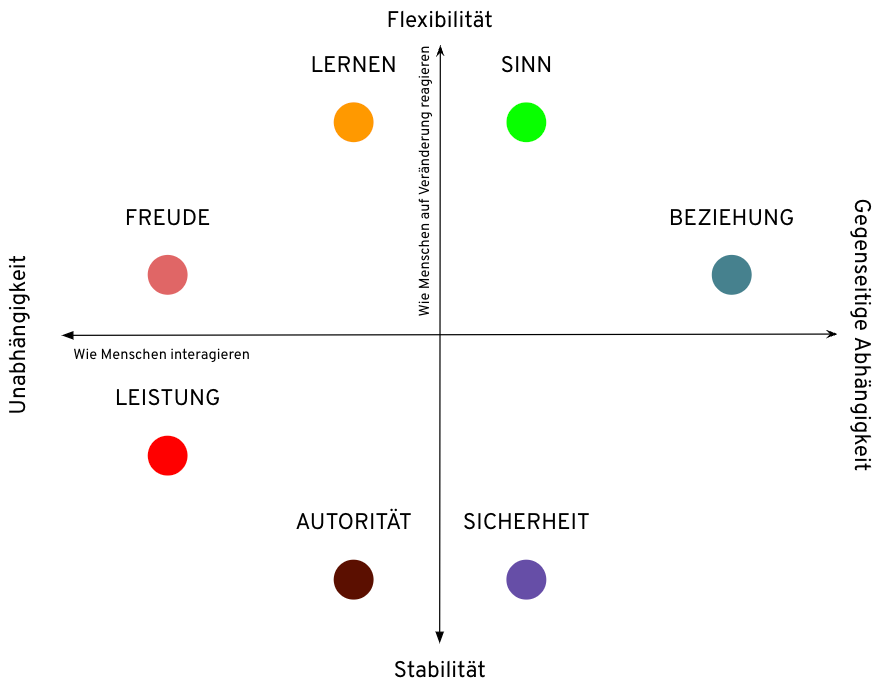
\includegraphics[width=0.8\linewidth,height=\textheight,keepaspectratio]{images/figure411.png} \hfill{}

\caption{Abb. 4.11: Integrated Culture Framewor (Credits: Spencer
Stuart, In: Groysberg et al., 2018b, S. 47)}

\end{figure}%

Von den Autor:innen wird betont, dass diejenigen Kulturstile, die weit
auseinander liegen, tendentiell auch schwerer miteinander in Einklang
gebracht werden können. In der Befragung der Unternehmen wurde
festgestellt, dass insbesondere die Leistungsorientierung (89\% der
Unternehmen) und Beziehungsorientierung (63\% der Unternehmen) am
häufigsten vorzufinden sind, gefolgt von Ordnungs- und Sinnorientierung
(Groysberg et al., 2018b, S. 49).

\subsection{Analyse von
Organisationskulturen}\label{analyse-von-organisationskulturen}

Ein hilfreiches Werkzeug für die Entwicklung von Organisationskulturen
stellt die SWOT-Analyse (Stärken-Schwächen-Chancen-Risiken) dar. Bei den
Stärken kann grundsätzlich danach gefragt werden: Was machen wir in der
Organisation schon gut? Worauf sind wir stolz? Was motiviert uns? Und
wie sieht die aktuelle Situationslage aus? Bei den Schwächen könnten
eine Selbstüberprüfung hilfreich sein: Wo gibt es Barrieren? Welche
Konflikte, die uns immer wieder prägen, gibt es in der Einrichtung? Wo
muss eine grundsätzliche Lösung gefunden werden? Bei den Chancen geht es
um die Fragen wie: Welche Ressourcen sind vorhanden und welche müssen
vielleicht zukünftig noch weiterentwickelt werden? Wie können wir die
Kompetenzen innerhalb der Einrichtung zukünftig noch weiter ausbauen?
Dies kann z. B. durch Weiterbildungen, die Durchführung von Projekten,
oder die Kooperation mit anderen Partnern erreicht werden. Bei den
Bedrohungen und Risiken kann man sich die Frage stellen, was es denn
grundsätzlich für Schwierigkeiten und Rahmenbedingungen gibt, die wir
beachten müssen? Risiken sind negative Einflüsse, die „von außen''
kommen und die uns gewissermaßen dazu zwingen, die Organisationskultur
weiterzuentwickeln: Welche Risiken gibt es, die aktuell bestehen oder
kritische Faktoren, die sich verändern müssen? Das können bspw.
gesetzliche, wirtschaftlicher Rahmenbedingungen oder dergleichen sein.
Diese Analyse kann dabei helfen, die Organisationskultur einer
Einrichtung aus unterschiedlichen Perspektiven zu beleuchten, zu
hinterfragen und daraus Schlussfolgerungen zu ziehen.

\subsection{„Pflege'' von
Organisationskulturen}\label{pflege-von-organisationskulturen}

Wenn man die etymologische Begriffsentwicklung von Kultur
zurückverfolgt, so stößt man im Altertum auf einen ergologischen
(\emph{ergos}: Arbeit) Kulturbegriff. Kultur war ursprünglich mit dem
Ackerbau verbunden. Damit war das Bestellen des Ackers bzw. die Aussaat
bzw. „Pflege'' des Feldes gemeint. Dieses Prinzip kann auf die
Organisationskultur übertragen werden. D. h., dass Leistungskräfte und
auch alle Mitarbeitende die Aufgabe haben, die Organisationskultur ihrer
Einrichtung mitzugestalten. Dies ist eine Aufgabe und ein Auftrag.

Wir müssen in unseren Organisationen also ständig über Werte und
Überzeugungen sowie die Haltungen, wie wir zusammenarbeiten, was unsere
Zusammenarbeit trägt und prägt, ständig im Gespräch bleiben. Eine
lebendige Organisationskultur, wenn sie sich denn kontinuierlich
entwickelt und dabei alle Beteiligten mitnimmt, führt letztlich dazu,
alle ihre Arbeit viel motivierter, mit höherem Engagement und häufiger
auch kreativer umsetzen. Eine solche „Pflege'' der Organisationskultur
kann schließlich in verschiedener Art und Weise erfolgen: \emph{Erstens}
ist die systematische Sicht, dass Kommunikation die Organisation von
innen prägt, von immenser Bedeutung. D. h. es muss darauf geachtet
werden, dass Mitarbeitende sich nicht nur um ihre eigenen Aufgaben
kümmern, sondern sich auch für das Team verantwortlich fühlen.
Leitungskräfte stehen hierbei in der Verantwortung, regelmäßig
Möglichkeiten für Gespräche anzubieten, sodass kontinuierlich die Vision
der Einrichtung kommuniziert wird: Wo wollen wir hin? Wo stehen wir
gerade? Warum ist der nächste Schritt wichtig? Alle sind an der
Weiterentwicklung der Zusammenarbeit beteiligt bzw. zu beteiligen.

\emph{Zweitens} sollte die Organisationskultur in den Strategien,
Strukturen und Prozessen verankert werden. D. h. in der
Strategieentwicklung bzw. -erweiterung sind entsprechend Mitarbeitende
einzubeziehen, sodass alle eine Information darüber haben, was denn die
nächsten Entwicklungsschritte sind. In den Prozessen muss verankert
werden, wo es regelmäßige Zusammenkünfte und Austauschmöglichkeiten gibt
(wie z. B. Beratungen, Reflektionsmöglichkeiten, Supervision,
Konfliktlösungsangebote)?

\emph{Drittens} sollte es eine Verankerung der Organisationskultur in
der Organisation- und Personalentwicklung geben.
Organisationsentwicklung und eben auch Organisationskulturentwicklung
ist stets auch verbunden mit Personalentwicklung. Um eine
Personalentwicklung zu gewährleisten, muss das Wissen, die Kompetenzen
sowie Fähigkeiten und Fertigkeiten der Mitarbeitenden stetig
weiterentwickelt werden.

\emph{Viertens} muss stets auch neuen Mitarbeitenden in der Einrichtung
die Organisationskultur bekannt „explizit'' werden (z. B. in Kick-off
Veranstaltungen, Mentor*innen oder Coachingprogrammen zu Arbeitsbeginn).

Und schließlich \emph{fünftens} wird eine Organisationskultur in
Ritualen gefestigt, wie z. B. durch Geburtstagsrunden, kollegiale
Beratungen, Pausengestaltung, teambildende Maßnahmen. Zusammenfassend
kann gesagt werden, dass die Gestaltung von Organisationskulturen von
allen Mitgliedern der Organisation eine regelmäßige Auseinandersetzung,
Wertschätzung, Flexibilität und ein „Im-Gespräch-Bleiben'' erfordert und
verschiedene zukunftsweisende Wege und Ebenen genutzt werden müssen.

\section{Organisationsanalyse}\label{organisationsanalyse}

\subsection{Überblick zur
Organisationsanalyse}\label{berblick-zur-organisationsanalyse}

In diesem Kapitel geht es um die Organisationsanalyse als Teil der
Situationsanalyse im Unternehmen. Die Organisationsanalyse ist ein
wichtiges Instrument, das man zur Planung von Veränderungsprozessen in
der Einrichtung nutzen kann. Diese hilft beispielsweise dabei, sich
einen Überblick über die aktuelle Situation und Lage der Organisation
sowie der damit zusammenhängenden Strukturen, Prozesse und Strategien zu
verschaffen. Dabei können unterschiedliche Dinge auf dem Prüfstand
stehen: z. B. Prozessstrukturen, die Organisationskultur oder
verschiedene andere Aspekte. Im Zuge der Ausführungen wird zunächst auf
Begriff, Ziele und Vorgehensweise allgemein eingegangen. Im Anschluss
daran werden die einzelnen Phasen beschrieben und folgende Fragen
geklärt: Was muss bei der Auftragsklärung beachtet werden? Wozu dient
die Beteiligten- bzw. Stakeholderanalyse? Welche Aspekte werden bei der
Analyse der Aufbau- und Ablauforganisation sowie der Organisationskultur
untersucht? Was kann man den betriebswirtschaftlichen Kennzahlen sowie
der Kostenanalyse entnehmen? Wie kann man eine Wettbewerbsanalyse
umsetzen? Wie können schließlich Veränderungsziele formuliert werden,
die letztlich in die Organisationsentwicklung einmünden werden?
Abschließend wird ein Ausblick auf verschiedene Methoden, die man im
Rahmen der Organisationsanalyse einsetzen kann, gegeben.

\subsection{Was ist
Organisationsanalyse?}\label{was-ist-organisationsanalyse}

Die Organisationsanalyse kann verschiedene Zielsetzungen bzw.
Fragestellungen verfolgen. Einen guten Einblick in die Ziel- bzw.
Aufgabenstellungen der Organisationsanalyse gewährt beispielsweise die
Definition von (Kolhoff, 2005, S. 6):

\begin{quote}
„Organisationsanalyse dient dazu, alle oder einzelne Systemelemente
einer sozialen Einrichtung oder eines sozialen Dienstes zu untersuchen,
um auf Veränderungen mit Verbesserungen reagieren zu können. Ziel der
Analyse ist neben -- gegenüber dem Ist-Zustand -- effizienteren und
effektiveren Aufbau- und Ablauforganisationen (technostrukturiert) auch
eine Verbesserung der Qualität der Arbeitsbedingungen der
Organisationsmitglieder (soziostrukturiert), um die Problemlösekapazität
der Organisationen zu erweitern und somit die notwendigen
Anpassungsleistungen zum Überleben auf einem zunehmend durch Konkurrenz
gekennzeichneten Markt erbringen zu können (systemstrukturiert).''
\end{quote}

Wie Kollhoff nahe legt, kann eine Organisationsanalyse auf
unterschiedlichen Ebenen stattfinden. In einer sozialen Einrichtung kann
diese entweder einzelne Aspekte oder die gesamte Organisation umfassen.
Sie dient grundsätzlich dazu, Grundlagen dafür zu schaffen, dass
organisationale Verbesserungen und Veränderungsprozesse angeregt werden.
Ziel der Analyse ist es, auf mindestens drei Ebenen aktiv zu werden: Das
ist einerseits die „Technostruktur'', welche auf die formale bzw.
administrative Struktur einer Einrichtung verweist. Damit ist
beispielsweise die Aufbau- und Ablauforganisation (also Organigramme
oder Prozessübersichten) gemeint. Verbesserungen soll es aber auch auf
anderen Ebenen geben, z. B. wo Arbeitsbedingungen der
Organisationsmitglieder geregelt werden. In letzterem Falle handelt es
sich um die „Soziostruktur''. Wie oben bereits dargestellt, sind
Organisationen soziale Gebilde. Darüber hinaus ist es möglich, dass,
wenn man Wissen über die Techno- und die Soziostruktur entwickelt hat,
zukünftig Probleme besser erkennen und lösen zu können. Mit der
Umsetzung der analysierten Veränderungsnotwendigkeiten und dem
schrittweisen Anpassungsprozess beschäftigt sich letztlich die
Organisationsentwicklung, die den Prozess umfasst, wie eine Organisation
sich den ständig veränderten Rahmenbedingungen des jeweiligen sozialen
Markts bzw. in deren internen und externen Umwelt anzupassen. Für den
Anpassungsleistungen ist beispielsweise eine Analyse der Konkurrenz-
bzw. Wettbewerbssituation im aktuellen sozialen Markt notwendig. Alle
analysierten Zusammenhänge, die die Wechselbeziehung zwischen
Organisation und der sie umgebenden Systemumwelt betreffen, wird durch
die sog. „Systemstruktur'' erfasst.

\subsection{Schritte der
Organisationsanalyse}\label{schritte-der-organisationsanalyse}

Um eine Organisationsanalyse durchzuführen, müssen schließlich
verschiedene Schritte geplant und umgesetzt werden, die im Folgenden
näher dargestellt werden: Im ersten Schritt der Organisationsanalyse
erfolgt die Besprechung und letztlich eine Erteilung des konkreten
Analyseauftrags und dabei sind Fragen zu klären wie: Wer ist überhaupt
dafür zuständig, wie sieht der Zeit- und Ablaufplan aus, bis hin zu der
Frage, welche Aspekte müssen in der Analyse erfasst werden. In der
zweiten Phase geht es darum, eine Beteiligten- bzw. Stakeholderanalyse
(hier werden beide Begriffe synonym verwendet) durchzuführen: D. h.,
alle Stakeholder (=Interessenbeteiligten) sind in den Analyseprozess
einzubeziehen. Am Ende dieses zweiten Schritts muss eine
Steuerungsgruppe gebildet werden. Im dritten Schritt geht es darum, die
Aufbau- und Ablaufstruktur sowie die Organisationskultur, inklusive des
Führungsverhaltens und der Mitarbeitersituation, zu untersuchen. Mit
anderen Worten geht es hier um die Techno- und Soziostruktur der
Organisation.

Im vierten Schritt geht es in der Organisationsanalyse darum, eine
Wettbewerbsanalyse bzw. Wettbewerbserkundung durchzuführen und damit die
Fragen zu klären: Wer und welche anderen Einrichtungen stehen
möglicherweise ebenfalls mit der gleichen Kundengruppen in Beziehung,
woraus entsprechende Veränderungsmaßnahmen abzuleiten sind? Die
Wettbewerbsanalyse kann man mit verschiedenen Methoden umsetzen: z. B.
Stärken-Schwächen-Chancen-Risiken-Analyse (SWOT) oder Portfolio-Analyse.
Darauf gehen wir später noch mal genauer ein. Wenn man diese ganzen
Phasen durchlaufen hat, oder Teile davon, sollte man am Ende eine Matrix
entwickeln, die verschiedene Vorschläge beinhaltet, was zukünftig in der
Organisation verändert werden muss: Welche Veränderungen sollen in
welchen Handlungsfeldern der Einrichtung umgesetzt werden?

Während wir in den Phasen 1 bis 4 den Ist-Zustand erfasst haben, geht es
abschließend im fünften Schritt darum, die Soll-Zustände zu definieren.
Der ermittelte Veränderungsbedarf ist schließlich wiederum Voraussetzung
für die zukünftige Organisationsentwicklung. Im Folgenden wird noch
einmal detaillierter auf die einzelnen Phasen eingegangen.

\subsubsection{Auftragsklärung}\label{auftragskluxe4rung}

Kommen wir nun im ersten Teil zu der Frage, wie die Auftragsvereinbarung
stattfindet. Man kann sich hier beispielsweise vorstellen, dass ein*e
externe*r Organisationsberater*in damit betraut werden soll, die
Organisationsanalyse durchzuführen. Ebenso lässt sich aber die
Vorgehensweise auch auf eine interne Organisationsanalyse übertragen.
Bei der Auswahl einer geeigneten Organisationsberatung müssen passende,
klar spezifizierte Vergleichsangebote eingeholt werden, die vorgelegten
Referenzen sowie die Kompetenzen der Berater*innen geprüft werden.
Besitzt die Person bereits Erfahrungen mit Einrichtung wie der unseren
bzw. der gleichen Branche. Im Auswahlprozess sollte darauf geachtet
werden, dass die Personen in der Lage sind, eine Vielzahl von Methoden
einzusetzen und entsprechende Kompetenzen mitbringen, die möglichst aus
dem gleichen Berufsfeld wie der untersuchten Einrichtung stammen. Dann
besteht eine höhere Wahrscheinlichkeit, dass die Berater*innen sich
besser in die Lage der Mitglieder der untersuchten Einrichtung zu
versetzen.

In den ersten Gesprächen mit den Verantwortlichen für die
Organisationsanalyse geht es erstens darum, einen IST-Stand zu erfassen.
Die dafür notwendigen Informationen, Zugänge zu Dokumenten und Kontakt
zu Mitarbeitenden sollte vorbereitet bzw. zur Verfügung gestellt werden,
um so eine Auftragsklärung vorzunehmen. Es geht dabei schlichtweg um die
Frage, wie ist es um die aktuelle Lage bestellt ist? Darüber hinaus
sollte auch geklärt werden, welche Methode eingesetzt wird, wie die
Grundarchitektur des Analyseprozesses aussehen kann und wie eine
Problemlösungsweg, der alle in der Beteiligung gleichermaßen
mitbeteiligt aussehen kann. Im Rahmen der Fixierung des Analyseauftrags
geht es zweitens auch darum festzulegen, welche Zielsetzungen im Rahmen
der Organisationsanalyse im Vordergrund stehen sollen: Wer ist wie
beteiligt? Wie ist der Prozess gestaltet, wie sieht der Weg der
Entscheidungsfindung bzw. Meinungsbildung aus? Es sollte von vornherein
überlegt werden, wem welche Informationen zugearbeitet werden müssen, um
nach erfolgter Organisationsanalyse den Prozess der
Organisationsentwicklung einzuleiten. Schließlich drittens sollten
schließlich die konkreten Analysemethoden festgelegt werden, um den
Prozess erfolgreich umsetzen zu können. Das sind jetzt drei ausgewählte
Dinge, natürlich keine vollständige Liste, die vereinbart werden müssen.

Schließlich muss auch die Frage geklärt werden, welche Daten und
Informationen der für die Organisationsanalyse verantwortlichen Personen
zur Verfügung gestellt werden müssen? Dabei kann es sich klassisch um
Dokumente mit betriebswirtschaftlichen Auswertungen, wie z. B.
Kennzahlen und Kostenstrukturen handeln. Hilfreich sind dabei alle
Statistiken mit Datenmaterial über das Unternehmen, das Leitbild,
Organigramm ein Überblick über das Leistungsangebot, die Zahl der
Mitarbeitenden, Evaluationen der Klient*innenzufriedenheit und
Datenmaterial zur Konkurrenzsituation (welche andere Unternehmen mit
ähnlicher Ausrichtung in der gleichen Region bzw. Stadt existieren.

Für die Strukturierung der Organisationsanalyse gibt es verschiedene
Vorschläge. Man unterscheidet einerseits in Analyseebenen und
andererseits in die Analysedimensionen. Mit den Analysedimensionen ist
der praktische Kontext der Organisationsanalyse gemeint: In welchen
Zeitraum wird was wann wie umgesetzt? Handelt es sich um eine Analyse
des gesamten Träger oder nur von Einrichtungsteilen bzw. einzelnen
Standorten?

Die Analyseebenen umfassen die verschiedenen Kriterien, auf die sich die
Organisationsanalyse beziehen soll: Beim Aufgabensystem spielen die
Arbeitsschwerpunkte und Arbeitszeiten bzw. die Arbeitskoordination
mittels entsprechender Arbeitsabläufe eine Rolle. Beim Aufgabenfeld geht
es darum, die Aufgaben, die üblicherweise in der Einrichtung anfallen,
auf den Prüfstand zu stellen. Im Rahmen der Prozessanalyse können die
Aufgabenträger eingegrenzt werden, d.~h. die zuständigen Personen in den
untersuchten Bereichen. Auf der Kommunikationsebene wäre zu fragen, wer
welche Informationen weitergeben bzw. Ansprechpartner in der
Organisation für bestimmte Aufgaben ist. Darüber hinaus kann man sich in
der Organisationsanalyse die personelle und sachliche Ausstattung der
Einrichtung genauer anschauen. Auf der Führungsebene geht es um die
Frage, wie Personalführungs- und Personalentwicklungsprozesse
ausgestaltet sind, z. B. Zielvereinbarungen, Entlohnungssystems,
Personalführungsstile, Mitarbeiterbesprechungen und
Entscheidungsfindungsprozesse. Ausschlaggebend für den Erfolg oder
Misserfolg einer Organisationsanalyse ist die Tatsache, ob die
Geschäftsleitung hinter dem Vorhaben steht oder nicht. Die Analyseebenen
und Analysedimensionen helfen dabei, den Analyseauftrag besser
einzugrenzen.

\subsubsection{Beteiligten- bzw.
Stakeholder-Analyse}\label{beteiligten--bzw.-stakeholder-analyse}

Im nächsten Schritt wird eine Beteiligten- bzw. Stakeholderanalyse
durchgeführt (beide Begriffe werden im Folgenden synonym verwendet).
Ziel der Analyse ist die Identifikation der Stakeholder, die im Rahmen
des Organisationsanalyseprozesses einbezogen werden sollen. Mithin
bietet diese Analyse die Möglichkeit, die oben dargestellten
Zusammenhänge der Multirationalität und Hybridität visuell darzustellen.
Eine Möglichkeit der Differenzierung unterschiedlicher Stakeholder ist
eine Tabelle, die zwischen Internen und Externen unterscheidet. Eine
andere Möglichkeit stellt ein Koordinatensystem dar, in den
unterschiedlichen Kriterien einander gegenübergstellt werden, z. B.
geografische Nähe und Distanz zu förderlichen und nicht-förderlichen
Stakeholdern. Eine hilfreiche Ressource für die Suche nach Stakeholdern
stellt das St.~Galler Management-Modell dar, in dem bereits verschiedene
Gruppen definiert wurden. Die Stakeholder-Analyse besteht aus vier
Prozessschritten.

Im ersten Schritt geht es um die Identifikation aller möglichen
beteiligten Personen und Gruppen, die mit der Organisation in Beziehung
stehen. Im zweiten Schritt geht es darum, zu definieren, wie bestimmte
Personen oder Gruppen, die ähnliche Interessen und Zielstellungen
verfolgen, zu einer Kategorie bzw. einem Cluster zusammengefasst werden
können, z. B. Leitungskräfte, Nutznießer bzw. Begünstige, Zielgruppen
bzw. Klient*innen, Finanziers, Kooperationspartner. Drittens müssen die
verschiedenen Erwartungen, Interessen, Beteiligungs- und
Einflussmöglichkeiten der einzelnen im ersten und zweiten Schritt
identifizierten Stakeholder erfasst werden. Daraus lassen sich später
die Interaktionsthemen -- wie im St.~Galler Management-Modell
dargestellt -- ableiten. Schließlich viertens kann auf Basis der
Informationen eine Steuerungsgruppe gebildet werden, die für den Prozess
der Organisationsanalyse entsprechend Verantwortung tragen wird bzw.
diesen unterstützt und berät. In der Steuerungsgruppe können
Mitarbeitende und Leitungskräfte der Einrichtung ebenso einbezogen
werden wie Externe. Die Steuerungsgruppe hat u. a. die Aufgabe, alle
notwendigen Entscheidungen für die Umsetzung der Analyse zu treffen, die
erhobenen Daten auszuwerten, zu interpretieren und zu diskutieren,
Veränderungsziele zu formulieren und den Gesamtprozess zu steuern.

\subsubsection{Analyse der Organisationsstruktur, -prozesse und
-kultur}\label{analyse-der-organisationsstruktur--prozesse-und--kultur}

Im nächsten Schritt wird die Ablauf- und Aufbaustruktur der Einrichtung
analysiert. Angeknüpft werden kann hierbei einerseits an die
verschiedenen Organigramme, z. B. (Stabs-)Linien, Produkt- und
Matrixstruktur, die eine Organisation dabei unterstützen,
Verantwortlichkeiten und Aufgabenbereiche zu definieren. Darüber hinaus
sind auch Stellen- bzw. Tätigkeitsfeldbeschreibungen hilfreich, um
daraus Informationen über die Unter-/ Überordnung von Aufgabenfeldern zu
gewinnen. Im Rahmen der Analyse der Ablauforganisation geht es um die
Frage, welche Mitarbeitende wie organisatorisch eingebunden sind und
welche Dokumentations- und Kommunikationswege existieren.

Hilfreiche Analyseinstrumente stellen dabei beispielsweise Zeit- und
Dienstpläne dar. Gesetzt der Fall, in einer Einrichtung soll die
Notwendigkeit einer Fremdunterbringung geprüft werden, so kann man einen
Zeit- und Ressourcenplan sowie die Entscheidungswege darstellen, um
damit den IST-Stand des Prozesses darzustellen, woraus später
Veränderungsmaßnahmen abgeleitet werden sollen. Mithilfe eines solchen
Plans kann die Ablauf- und Aufbaustruktur visualisiert werden. Im
besagten Beispiel muss dargestellt werden, wie der Prozess von der
Anfrage zur Überprüfung im ersten Schritt über verschiedene Vermerke,
die in den einzelnen Fachbereichen bzw. Sachgebieten geprüft und
weitergereicht werden, bis zur endgültigen Entscheidung und dem Bericht
über die Notwendigkeit oder Ablehnung einer Fremdunterbringung gestaltet
ist, wie viele Zeit- und finanzielle Ressourcen dabei verbraucht werden.
Ein solcher Ablaufplan gibt einen klaren Überblick darüber, wer was in
welchem Sachgebiet mit welchen Ressourcen umsetzt. Auf Basis der Analyse
kann schließlich überlegt werden, welche Veränderungs- bzw.
Gestaltungsmöglichkeiten bestehen, um den Prozess ggf. ein wenig zu
vereinfachen, ohne damit professionelle Entscheidungskompetenz damit zu
gefährden.

Weiterhin kann man neben der Ablauf- und Aufbaustruktur, also der
Technostruktur einer Organisation, auch die Soziostruktur betrachten.
Dabei geht es um Fragen wie z. B.: Wie sehen die Arbeitsbedingungen aus,
welche Maßnahmen der Personalentwicklung gibt es. Im Rahmen der
systemischen bzw. systematischen Organisationsanalyse beschäftigt man
sich mit der Frage, welche Kommunikationsprozesse, Führungsstrukturen in
der Einrichtung existieren und auf welche Art und Weise Entscheidungen
überhaupt getroffen werden. Diese Informationen sind wichtig, um später
die Beziehungs- bzw. Interaktionsprozesse in Organisationen zu
untersuchen.

Viele Organisationsberatungsansätze beschäftigen sich mit der
Soziostruktur sowie den psychodynamischen Prozessen. Beispielsweise
werden in allen Organisationen sogenannte Spiel gespielt, die mitunter
zuträglich sein können aber überwiegend negative Effekte haben. Damit
sind keine Kartenspiele oder dergleichen gemeint, sondern Menschen
spielen miteinander in Organisationen um Ressourcen, Macht, Anerkennung
etc. Die bekanntesten Beispiele sind wohl die sog. Machtspiele, z. B.
wenn gegen ein Vorhaben bewusst Widerstandes geleistet wird, sich eine
Gruppe Mitarbeitender gegen eine Entscheidung auflehnt und nicht gewillt
ist, bestimmte Veränderungsmaßnahmen umzusetzen bzw. zu unterstützen.
Mit anderen Worten handelt es sich dabei um Widerstandsspiele. Darüber
hinaus gibt es auch Machtaufbauspiele, wo es darum geht, dass einzelne
Person in einer über besonderes (Experten-)Wissen verfügen. Manchmal
entwickeln sich Strukturen in der Einrichtung, wo für eine Beratung
nicht die Person gefragt wird, die formal gesehen dafür zuständig ist,
sondern eben die Person, die am besten darüber Bescheid weiß.
Erfahrungswissen und Funktion müssen nicht immer zusammenfallen. Ebenso
können sich in Einrichtungen Allianzen bilden, also Gruppen, die sich
sozusagen gemeinschaftlich für Ideen einsetzen. Weiterhin gibt es
Bekämpfungsspiele, in denen Entscheider*innen mit Experten, die sich in
einem Tätigkeitsfeld besonders gut auskennen in Verhandlung stehen,
diskutieren und aushandeln müssen. Schließlich gibt es
Veränderungsspiele, wenn Personen aufgrund von Insider- oder Vorwissen
über mehr Informationen verfügen und sich dadurch Vorteile gegenüber
Personen, die diese Informationen nicht haben, verschaffen. Das lässt
sich häufig in Verhandlungen zwischen Einrichtungsleitung,
Mitarbeitenden und Personalrat oder in politischen Gremien verfolgen.
Mit anderen Worten führen viele dieser Spiele dazu, dass die formale
Organisationstruktur und Organisationskultur unterwandert wird. Diese
Ausführungen sollen kein schlechtes Licht auf Organisationen richten,
vielmehr ist dies als eine Beschreibung der Realität zu analysieren und
zu verstehen. Eine andere Frage ist, wie man damit umgeht und die
Organisationskultur (um-/weiter-)gestaltet. Grundsätzlich gibt es bei
allen diesen Formen von Organisationsspielen auch positive Aspekte. Z.
B. kann eine Allianz dazu führen, dass eine wichtige Entscheidung
getroffen wird. Was allerdings problematisch ist, ist wenn Informationen
bewusst zurückgehalten werden damit die Transparenz gefährdet ist bzw.
kein Fairplay mehr stattfindet

Ebenso kann im Rahmen dieses Analyseschritts das Mitarbeiterverhalten,
mit anderen Worten das Zusammenspiel zwischen Mitarbeitenden und
Leistungskraft, untersucht werden: z. B. Beteiligungsmöglichkeiten an
der Strategie- bzw. Leitbildentwicklung, unterschiedliche Auslastungen
und Belastungen einzelner Mitarbeitenden, notwendige
Personalentwicklungsmaßnahmen zur Weiterqualifikationen des Personals,
Unterstützung intrinsischer Motivation der Mitarbeitenden. Darüber
hinaus spielt auch die Organisationskultur eine Rolle. So könnte man
fragen, welche ritualisierten gemeinsamen Feste und (wie oben erwähnt)
bestimmte Fördermöglichkeiten es gibt. Darüber hinaus gilt es Gründe für
ständige Fluktuationen zu finden bzw. Aktivitäten des Arbeitgebers zur
Mitarbeiterbindung ausfindig zu machen. Schließlich sollte auch
analysiert werden, welche Maßnahmen zur Verbesserung bzw. Entwicklung
der Arbeitsbedingungen bzw. des Arbeitsplatzes zur Verfügung stehen.
Ebenso steht bei der Untersuchung des Mitarbeiterverhaltens die Frage
der Personalführung im Mittelpunkt: z. B. welche Führungsansätze werden
gelebt, autoritäre bzw. autoritative, demokratisch geprägt. Aus allen
diesen Aspekten lässt sich am Ende des Analyseprozesses ein
Veränderungsbedarf ableiten.

\subsubsection{Kostenanalyse}\label{kostenanalyse}

Im Rahmen der Kostenanalyse werden die Informationen und Daten des
Rechnungswesens und Controllings analysiert. Dabei geht es darum,
herauszufiltern, welche Tätigkeiten denn welche Kosten aufwerfen. Es
geht auch darum, Kostentreiber zu identifizieren und Ursachen für
ineffizienten Veränderungen in der Kostenstruktur aufzudecken, z. B.
wenn die fixen Kosten durch ungünstige Verträge gestiegen sind, zu hohe
Sozialleistungen anfallen, die möglicherweise auf einen hohen
Krankenstand zurückzuführen sind. Ineffizienzen in der
Organisationsstruktur und in den Abläufen kann man in der Regel auch in
der Kostenstruktur der Einrichtung nachvollziehen. Als Datenquellen kann
man zum Beispiel Betriebsabrechnungsbögen und
Wirtschaftlichkeitsabrechnungen verwenden, um herauszufinden, wo welche
kosten und wofür anfallen. Hintergrund der Kostenanalyse ist es weniger,
einfach blind Rationalisierungsmaßnahmen zu entscheiden, sondern die
Ursachen für Veränderungen zu identifizieren. Dies ist stets mit der
Frage verbunden: Wo können wir in unserer Einrichtung noch besser
werden, um damit besser unsere Aufgaben- und Zielstellung bzw.
Einrichtungszweck zu erfüllen?

\subsubsection{Wettbewerbs- bzw.
Konkurrenz-Analyse}\label{wettbewerbs--bzw.-konkurrenz-analyse}

Im Rahmen der Wettbewerbs- bzw. Konkurrenz-Analyse werden vier
Instrumente eingesetzt, die im Folgenden kurz erläutert werden sollen.
\emph{Erstens} gibt es die sogenannte Potenzialanalyse, bei der die
unternehmensinternen Kompetenzen, wie z. B. die Qualifikation des
Personals, Finanzen und Kostenstruktur analysiert werden (vgl. alle
vorherigen Schritte der Organisationsanalyse). Mit anderen Worten werden
die eigenen Ressourcen, die Aufgabenbereiche und Strategien dargestellt.
\emph{Zweitens} gibt es die Konkurrenzanalyse: Dabei fragen wir danach,
welche Zielgruppen eigentlich von den Einrichtungen bedient werden, wie
man diese mit anderen Einrichtungen der gleichen Region, der gleichen
Stadt oder des gleichen sozialen Marktes vergleichen kann. Außerdem wird
danach gefragt, ob sich bestimmte Bedarfe verändert haben, oder ob es
Hinweise darauf gibt, ob sich die Struktur des Klientels verändert hat.
\emph{Drittens} kann eine Stärken-Schwächen-Analyse durchführt werden,
mit deren Hilfe nach dem Innen des Unternehmens geschaut wird. Dies kann
durch Einsatz eines Fragebogens geschehen oder im Rahmen eines
Workshops, im dem die Ressourcen, wirtschaftliche Situation,
Personalbestand etc. erfasst und dokumentiert wird. \emph{Viertens} gibt
es die Portfolio-Analyse. Dabei geht es darum, dass nicht nur die Innen-
und Außensicht aufgenommen wird. Dabei steht die Frage im Vordergrund,
wie wir mit unseren Dienstleistungen im jeweiligen sozialen Markt
positioniert sind. Die Idee zur Portfolio-Analyse kommt aus den
Finanzwissenschaften: Portfolio heißt, dass wir so eine Art Warenkorb
haben, indem wir unterschiedliche Geschäftsfelder zusammengefasst sind
(z. B. Altenheim, Jugendhilfeeinrichtung, Wohngruppen,
Kindertageseinrichtung). Jede dieser Einrichtungen eines Trägers trägt
in unterschiedlicher Weise zur Entwicklung der Einrichtung bei. Diese
Methode verschafft damit einen Überblick über die verschiedenen
Geschäftsfelder und visualisiert, welche Position unsere Einrichtung im
Wettbewerb besitzt. Ein Vergleich mit anderen Einrichtungen ermöglicht
die Herausarbeitung des sog. USP (Unique Selling Proposition) bzw. von
Alleinstellungsmerkmalen oder Kernkompetenzen.

\subsubsection{Erarbeitung von Soll-Vorschlägen für
Handlungsfeldveränderungen}\label{erarbeitung-von-soll-vorschluxe4gen-fuxfcr-handlungsfeldveruxe4nderungen}

Im letzten Schritt der Organisationsanalyse findet die Zielbestimmung
statt. Nachdem nun in den vorherigen Phasen der aktuelle IST-Zustand
ermittelt wurde, muss in diesem letzten Schritt der gewünschte
Sollzustand bzw. die Ziele für die umzusetzenden Veränderungen
beschrieben werden. Dies kann in zwei Schritten erfolgen, erstens in
Gestalt des \emph{Ursache-Problem-Wirkungsbaums} oder zweitens durch
eines \emph{Reframings im Handlungsmöglichkeiten-Ziel-Wirkungsbaum}.

Im \emph{Ursache-Problem-Wirkungsbaum} geht es darum, ausgehend von den
Wirkungen, das dahinterliegende Kernproblem zu identifizieren, warum
bestimmte Abläufe oder Strukturen ineffizient sind. Aus dem Kernproblem
lassen sich dann verschiedene Ursachen ableiten, die verantwortlich
dafür gewesen sind, dass Probleme aufgetreten sind. Mit anderen Worten
handelt es sich um eine dreischichtige Problemanalyse, die im Folgenden
anhand eines Beispiels beschrieben werden soll. Es wurde festgestellt,
dass in die Arbeit des Jugendamts ein Vertrauensverlust entstanden ist,
was daran abgelesen werden kann, dass Klient*innen das Jugendamt meiden
und sich „allein gelassen'' fühlen. Wenn man danach fragt, was dabei das
eigentliche Kernproblem darstellt, kann relativ schnell erfasst werden,
dass die Klient*innen unzufrieden sind mit den Leistungen des
Jugendamts. Ursachen für diese Unzufriedenheit sind bspw. lange
Wartezeiten, unfreundliche Mitarbeitende und unzureichende Beratung. Aus
diesen Ursachen lässt sich die Unzufriedenheit der Klient*innen
schließen. Wenn wir weiter fragen, wie die Unfreundlichkeit der
Mitarbeitenden erklärt werden kann, lässt sich das darauf zurückführen,
dass dieser aktuelle Zustand im Jugendamt möglicherweise auf die
fehlende Motivation der Mitarbeitenden aufgrund ihrer geringe
Eigenverantwortlichkeit (Sozialstruktur) sowie lange, bürokratische Wege
(Technostruktur) zurückzuführen ist.

Mithilfe des \emph{Reframing-Ansatzes} gehen wir von der veränderten
Wirkungsbeschreibung über die neue Zielstellung hin zu den zu planenden
Interventionsmöglichkeiten und einzusetzenden Ressourcen. Damit wird
gewissermaßen das vorherige Bild noch einmal umgekehrt. Durch die neuen
Handlungsmöglichkeiten wird dann eine andere Wirkung erzielt. Dies sei
wieder anhand eines Beispiels erläutert: Zunächst muss die veränderte
Wirkung bzw. der Sollzustand definiert werden. Wir wollen erreichen,
dass zukünftig eine vertrauensvolle Zusammenarbeit mit den Klient*innen
ermöglicht wird. Das kann letztlich nur gelingen, wenn diese das
Jugendamt „angstfrei'' aufsuchen können und das Amt als „Partner'' und
weniger als eine (Verwaltung-)Behörde betrachten. Um diese gewünschte
Wirkung zu erzielen, muss bei allen Prozessen und Maßnahmen darauf
geachtet werden, dass die Zufriedenheit der Klient*innen gesteigert wird
(Zielebene). Das Amt entscheidet nicht über die Klient*innen hinweg,
sondern das Verhältnis wird als Co-Konstruktion von sozialer
Wirklichkeit verstanden. Um dieses Ziel umzusetzen, bedarf es
schließlich einer zügigen Bearbeitung der einzelnen Anträge, eines
freundlichen Gegenübertretens und einer umfassenden Beratung.
Freundliche und motivierte Mitarbeitende wird es nur dann geben, wenn
diese durch mehr Eigenverantwortung ausgestattet werden und es kurze,
überschaubare Verwaltungswege gibt.

\subsection{Methoden der
Organisationsanalyse}\label{methoden-der-organisationsanalyse}

Hinsichtlich der Auswahl geeigneter Methoden für die
Organisationsanalyse ist zunächst auf die Analysedimensionen und die
verschiedenen Ansätze im Rahmen der empirischen Sozialforschungsmethoden
einzugehen. Hinsichtlich der \emph{Analysedimensionen} sind insbesondere
die Struktur-, Prozess- und Ergebnisqualität von Belang. Im Kontext der
Strukturqualität stellt sich die Frage, inwieweit die Aufbau- bzw.
Organisationsstruktur der Einrichtung umgesetzt wird. Bei der
Prozessqualität stehen die Abläufe innerhalb der Institution im
Vordergrund. Und bei der Ergebnisqualität untersuchen wir, wer wann wie
in der Einrichtung tätig ist bzw. zum Erfolg der Einrichtung beigetragen
hat. Hierbei ist außerdem zu fragen, welche Kriterien angelegt werden
können, um den Erfolg zu messen.

Hinsichtlich der verschiedenen \emph{Sozialforschungsmethoden} ist
zunächst zu fragen, welche Untersuchungsperspektive einzunehmen ist:
entweder qualitativ-orientierte Verfahren, die stärker auf eine
Exploration, Hypothesenbildung, Einzelfallanalyse, Untersuchung sozialer
Repräsentationen und Sinnzusammenhänge abzielen, oder umgekehrt im Sinne
quantitativer Sozialforschung, die auf eine Überprüfung von
theoretischen Zusammenhängen und Hypothesenüberprüfung abzielen. Je
nachdem könnten dann Befragungen und Experimente (stärker quantitativ)
oder Beobachtungen und Inhaltsanalyse (stärker qualitativ) eingesetzt
werden. Je nachdem welches verfahren wir wählen oder welchen Weg wir
gehen, sind auch bestimmte Methoden besser geeignet. Kurz
zusammengefasst geht es sozusagen bei der qualitativ-orientierten
Methodik um Hypothesenbildung und bei der quantitativ-orientierten
Methodik um eine Hypothesenüberprüfung.

Wie bereits festgestellt, gibt es eine große Bandbreite von Methoden,
die in der Organisationsanalyse eingesetzt werden können. Im Rahmen der
\emph{quantitativen Ansätze} können z. B. Aktenanalysen, Erhebungsbögen,
Vermerke, Verfügungen, Berichte, Gutachten, Briefe eingesetzt werden, um
dokumentierte Prozesse innerhalb der Einrichtung nachvollziehen zu
können. Mithin eigenen sich dabei auch die verschiedenen Dokumente des
Qualitätsmanagements. Dabei können unterschiedliche Foki eingenommen
werden: Bei der Frequenzanalyse wird nach der Häufigkeit und Intensität
bestimmter festgestellter Beobachtungen gefragt (z. B. Häufigkeit
bestimmte Fälle, Entscheidungen) oder im Sinne einer ABC-Analyse nach
Gewichtungen und Priorisierungen gefragt (z. B. wie hoch ist die
Relevanz und Priorität bestimmter Fälle, während A die höchste und C die
niedrigste Priorität besitzt). Bei Valenzanalysen wird versucht, die
Wichtigkeit zu bewerten. Valenz heißt, dass wir uns mit dem Wert
beschäftigen, etwas bewerten wollen (wie z. B. Mitarbeiterbefragungen).
Bei der Kontingenzanalyse werden Zusammenhänge untersucht bzw. die
Verbindung zwischen Elementen versucht herzustellen, um damit nach
Ursachen zu fragen und Wirkungen besser beurteilen zu können. Dabei
können beispielsweise Beschreibungen und Erklärungen von Akteninhalten
und Dokumenten gesucht werden, die uns in die Lage versehen,
Zusammenhänge zu erkennen.

Mit Hilfe der \emph{qualitativen Verfahren} geht es dann darum,
Einzelpersonen oder Gruppen zu befragen und an deren Sichtweisen und
Expertisen anzuknüpfen. Dazu sind bspw. mündliche Befragungen geeignet,
wie z. B. Individualinterviews, Gruppendiskussionen. Es lassen sich aber
auch schriftliche Befragung (z. B. per E-Mail oder Fragebogen)
einsetzen, allerdings nicht im Sinne eines strukturierten Fragebogens,
sondern mit möglichst offenen Fragen, die einen breiten Antwortraum
ermöglichen. Außerdem können Beobachtungen durchgeführt werden und auch
Tagesberichte analysiert werden, um damit Aufschluss zu bekommen für
über die verschiedenen Abläufe und Tätigkeiten, die eine Person oder
mehrere Personen während des Tages ausüben. Das ist eine wertvolle
Methode für Arbeitsanalyse z. B. im Rahmen von Abschlussarbeiten. Bei
der Tagesberichterfassung wird eine strukturierte Beobachtung
durchgeführt, in dem Daten der Gesprächsperson (Name, Abteilung, Raum,
Datum, Kontaktdaten) und für alle (Teil-)Aufgaben während des Tages die
jeweils benötigte Zeit (in Minuten/Sekunden), Arbeitsmittel,
Ansprechpartner, Einzeltätigkeit, Besprechung oder Zusammenarbeit
differenziert erfasst werden. Damit ist es möglich, ein genaueres Bild
von den tatsächlichen Arbeitsabläufen, Interaktionen und Arbeitsinhalten
während des Alltags zu erhalten. Diese Erkenntnisse können dann einen
Ausgangspunkt für Prozess- und Strukturanalyse, aber für die
Organisationskultur darstellen.

\section{Organisationsentwicklung}\label{organisationsentwicklung}

\subsection{Was ist
Organisationsentwicklung?}\label{was-ist-organisationsentwicklung}

In diesem Abschnitt beschäftigen wir uns mit der
Organisationsentwicklung. Was fällt Ihnen zu der Fragestellung: „Was ist
Organisationsentwicklung?'' ein. Bitte überlegen Sie kurz und notieren
Ihre Ideen.

Bei der Auseinandersetzung mit dem Begriff „Organisationsentwicklung''
soll uns folgende Definition der Gesellschaft für
Organisationsentwicklung behilflich sein:

\begin{quote}
„Organisationsentwicklung kann man allgemein als einen längerfristigen
angelegten Entwicklungs- und Veränderungsprozess von Organisationen
verstehen, der in nun tätigen Mitarbeitenden und Menschen. Der Prozess
beruht auf Lernen aller Betroffenen durch direkte Mitwirkung und
praktische Erfahrung. Sein Ziel besteht in der gleichzeitigen
Verbesserung der Leistungsfähigkeit der Organisation (Effektivität) und
der Qualität des Arbeitslebens (Humanität)'' (Gesellschaft für
Organisationsentwicklung zit. in Kolhoff, 2009).
\end{quote}

Was können wir aus dieser längeren Definition herausarbeiten?
Grundsätzlich kann man sagen, dass Organisationsentwicklung einen
längerfristigen Prozess darstellt:

\begin{itemize}
\item
  wie verändern sich Einrichtungen,
\item
  Entwicklungs- und Veränderungsprozess von Organisationen sowie
\item
  Ermittlung von notwendigen, zukünftigen Veränderungen.
\end{itemize}

Es sind nicht nur Strukturprozesse innerhalb der Organisation die sich
verändern, sondern es muss auch auf der Ebene der Mitarbeitenden
mitgedacht werden, wie der Veränderungsprozess umgesetzt werden kann. D.
h., Hintergrund der Organisationsentwicklung ist, den Prozess der
Veränderung in Organisationen sowie im Verhalten und der Einstellung von
Mitarbeitenden herauszufinden. Der Prozess der Veränderung bedeutet für
alle Betroffenen, dass diese die Veränderung mit umsetzen und für sich
verbindlich erklären müssen. Dies sollte durch Mitwirkung geschehen und
es sollten selbstverständlich auch praktische Erfahrungen mit einfließen
dürfen. In Ergänzung zu o. g. Definition gibt es verschiedene
theoretische und praktische Modelle, die man nutzen kann, um eine
Organisationsentwicklung umsetzen zu können (wie z. B. das
Dreiphasen-Modell von Kur Lewin; siehe Abschnitt 1.2.4. Im letzten Satz
der Definition ist noch etwas zur Zielsetzung ausgesagt: Warum tun wir
das? Wir wollen etwas verbessern, wir wollen die Zusammenarbeit
innerhalb der Organisation verändern, was dazu führt, dass wir hinterher
besser unseren Aufgaben gerecht werden können. Hier wird von
Leistungsfähigkeit der Organisation und Effektivität gesprochen, d.~h.,
wir müssen die Organisationsentwicklung auch in dieser Richtung
verstehen: Wir versuchen, unsere Ziele, unsere Strategien und die
Organisationskultur, unsere Prozesse und Strukturen zu optimieren bzw.
an unseren jeweiligen Leistungsauftrag anzupassen. Letztendlich geht es
auch um die Qualität des Arbeitslebens bzw. des Zusammenarbeitens. Wir
versuchen Organisationsentwicklung auch deswegen einzusetzen, weil sich
unsere Einrichtung und wir uns als Mitarbeitende ganz allgemein
innerhalb dieser Einrichtung weiterentwickeln wollen.

\subsection{Erfolgsfaktoren im Rahmen der
Organisationsentwicklung}\label{erfolgsfaktoren-im-rahmen-der-organisationsentwicklung}

Man kann sich fragen, wie solche Organisationsentwicklungen erfolgreich
sein können oder werden. Es gibt verschiedene Untersuchungen, die zu
ähnlichen Ergebnissen bei der Fragestellung gekommen sind, woran die
Erfolgsfaktoren festgemacht werden können und ob eine
Organisationsentwicklung zu dem gewünschten Ziel geführt hat. In den
Untersuchungen wurden verschiedene Aspekte genannt, die Aussage dazu
treffen, dass z. B. Barrieren und Grenzen zwischen den Mitarbeitenden
überwunden werden, dass Betroffene einbezogen werden sollen, dass
konsequent an der Problemlösung gearbeitet werden muss und dass man
Kenntnis über die Zusammenhänge der jeweiligen Veränderungsprozesse
haben soll. Des Weiteren ist dabei die Bedeutung der Kommunikation für
den Prozess der Veränderung noch einmal hervorgehoben und letztendlich
auch die aktive Unterstützung des Topmanagements, also der Leitung des
Trägers. Auch werden verschiedene Einfluss- und Erfolgsfaktoren
deutlich, die dazu führen, dass wir mit der Organisationsentwicklung zu
unserem Ziel kommen. Es sind grundsätzlich personalrelevante oder
personenrelevante Informationen (vgl. Wöhrle, 2012, S. 24)
(\hyperref[figure412]{Abb. 4.12}). Es sind sozusagen die Mitarbeitenden
und die Mitglieder von Organisationen selbst, die beteiligt werden
müssen und die offen kommunizieren sowie mit einbezogen werden müssen,
damit die Organisationsentwicklung gelingt. D. h., der „Faktor Mensch''
ist hier von besonderer Bedeutung für den Erfolg.

\begin{figure}

\pandocbounded{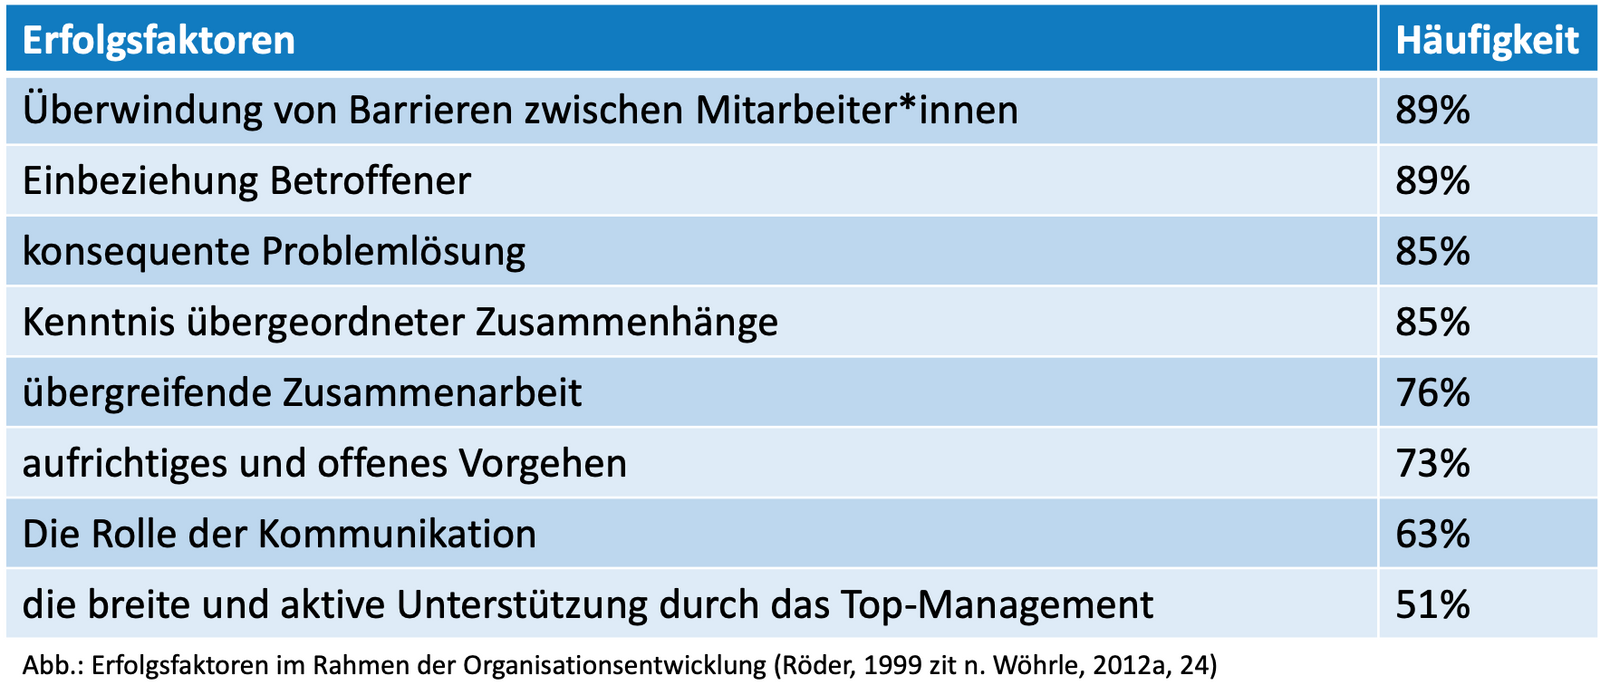
\includegraphics[keepaspectratio]{images/figure412.png}} \hfill{}

\caption{Abb. 4.12: Erfolgsfaktoren im Rahmen der
Organisationsentwicklung (Röder 1999, zit. n. Wöhrle, 2012, S. 24)}

\end{figure}%

Es gibt verschiedene Studien, die versuchen zu belegen, dass der
Großteil von Organisationsentwicklungsprozessen in der Regel schief
gehen, d.~h., dass man nicht die Ziele erreicht, die man hätte erreichen
wollen. Auch wenn es schwierig ist, dies methodisch festzustellen, geht
man davon aus, dass man nur bei einem kleinen Prozentsatz - einige sagen
30 oder gar 40 \% der Fälle - von einem Erfolg in der
Organisationsentwicklung im eigentlichen Sinne ausgehen kann. Die
bedeutet, dass sich die Schere für den tatsächlichen Erfolg am Ende des
Entwicklungsprozesses zwischen 30 \% und 70 \% bzw. 40 \% und 60 \%
bewegt.

\subsection{Formen des
Organisationswandels}\label{formen-des-organisationswandels}

Im Folgenden befassen wir uns nun mit den verschiedenen Formen des
Organisationsveränderungsprozesses. Einen Überblick gibt dabei die
\hyperref[figure413]{Abb. 4.13} (Wöhrle, 2012, S. 9), die zwischen der
ersten und der zweiten Ordnung unterscheidet.

\begin{figure}

\pandocbounded{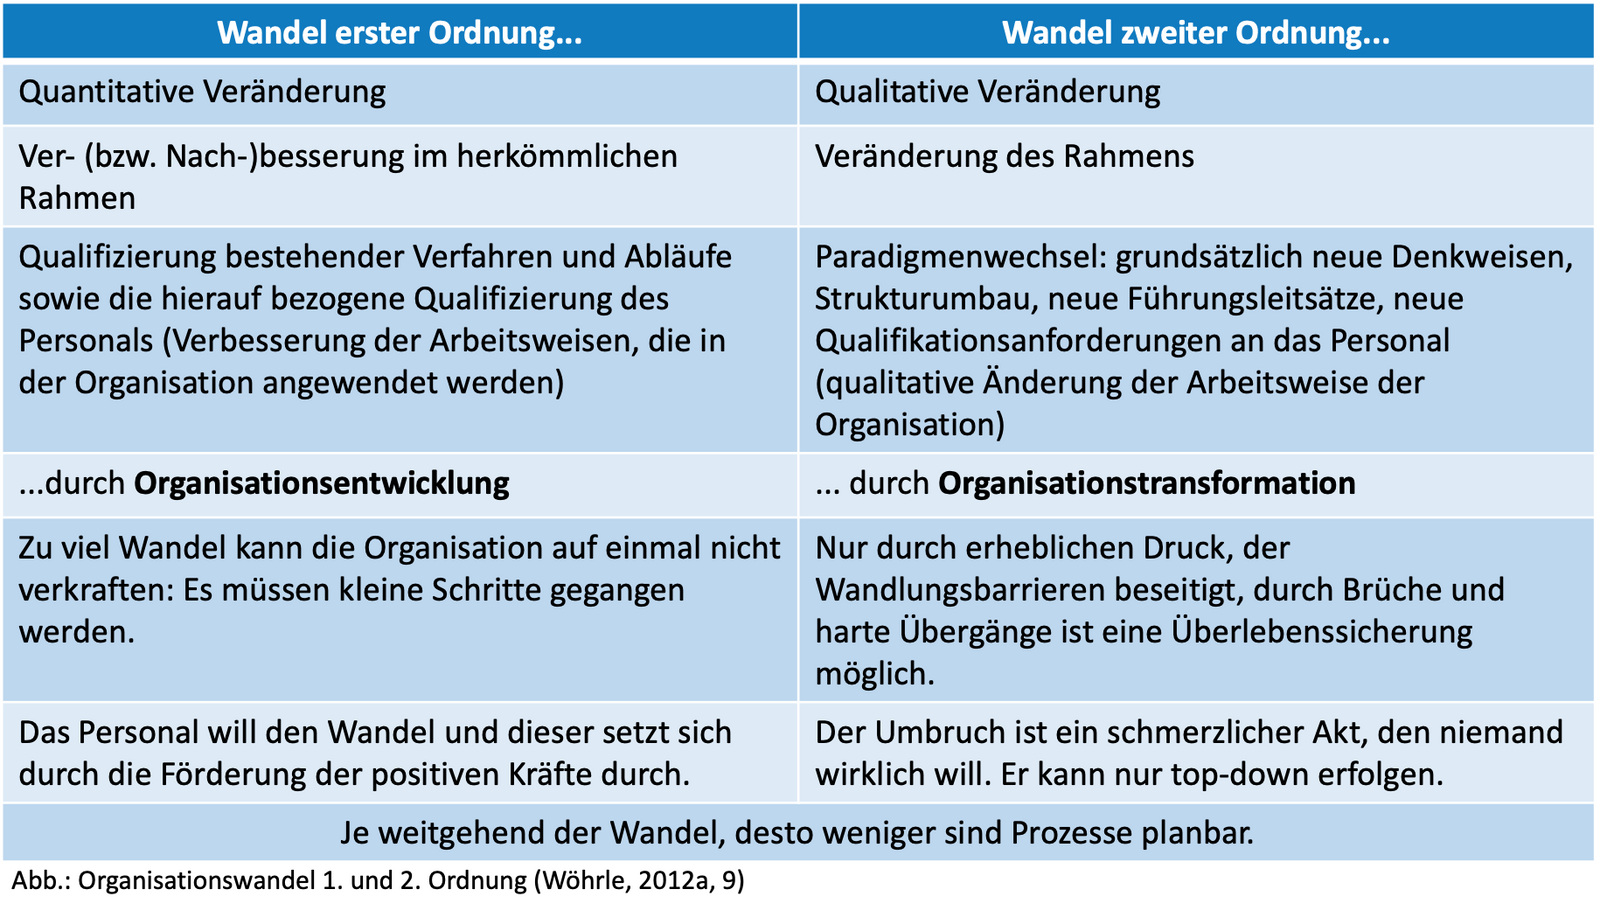
\includegraphics[keepaspectratio]{images/figure413.png}} \hfill{}

\caption{Abb. 4.13: Organisationswandel 1. und 2. Ordnung (nach Wöhrle,
2012, S. 9)}

\end{figure}%

In \hyperref[figure413]{Abb. 4.13} zum Kultur- bzw.
Organisationskulturbegriff wurde bereits schon einmal bei der
partizipatorischen Strategie auf die zweite Ordnung eingegangen, welche
nun noch einmal im Detail erläutert wird. Wenn wir einen Wandel zwischen
erster und zweiter Ordnung unterscheiden, dann ist der Wandel in der
ersten Ordnung so etwas wie eine qualitative Veränderung, eine
Optimierung im weitesten Sinne. Wir nehmen Verbesserungen an Strukturen,
Prozessen und an Strategien vor, unter Beachtung der aktuellen
Rahmenbedingungen, denn die Grundsätze und der Zweck der Einrichtung
sind nicht anzutasten. Das kann durch Qualifikation und nach
Qualifikationen der Einrichtungsmitglieder passieren. Verfahren,
Prozesse, Abläufe und Strukturen werden weiterentwickelt,~\emph{ohne die
grundsätzliche Idee, das grundsätzliche Organigramm zu verändern}.
Organisationsentwicklung meint hier im engeren Sinn, dass wir uns auf
der Ebene der ersten Ordnung befinden. Organisationsentwicklung ist ganz
allgemein der Prozess zur Umsetzung von Veränderung. Gleichzeitig hat er
eine zweite Bedeutung inne. Dabei geht es um Veränderungsmaßnahmen, die
der Optimierung dienen und die mit kleinen schrittweisen Veränderungen
einhergehen, sei es durch Politik oder Wandel innerhalb der ersten
Ordnung. Dabei muss letztendlich das Personal mitgenommen bzw. in den
Prozess einbezogen werden sowie regelmäßig motiviert und hinsichtlich
ihrer Ressourcen weiter unterstützt werden.

Mit dem Wandel auf der zweiten Ordnung ist gemeint, dass sich die
Organisation durch~\emph{qualitative}~Veränderung weiterentwickelt und
hierbei nun auch der Rahmen der Einrichtung hinterfragt wird, also die
grundsätzliche Struktur, die grundsätzlichen Missionen der Einrichtung,
die grundsätzlichen Leistungsbereiche.~\emph{Diese werden erweitert oder
gegebenenfalls auch komplett verändert}. Im weiten Sinne findet so etwas
wie ein Paradigmenwechsel statt. Diese Veränderungen führen zu neuen
Denkweisen, zu neuen Strukturen oder zu neuen Leitsätzen. In Folge
dessen muss das Personal an die neuen Rahmenbedingungen angepasst und
(nach)qualifiziert werden. Man spricht dabei auch von einer
Organisationstransformation. Transformation geschieht durch Überwindung
von Barrieren. Dabei werden Brüche innerhalb der Organisation entstehen
und gegebenenfalls auch ein gewisser Handlungsdruck, der von innen und
von außen kommen kann. Dies ist aber für den Wandel in der Organisation
bedeutsam, damit dieser auch in Gang kommen kann und damit letztendlich
das Ziel der Überlebenssicherung dieser Organisation erreicht wird.

Ein Wandel auf der zweiten Ordnung ist dann nicht notwendig, wenn wir
diesen grundsätzlichen Veränderungsprozess nicht angehen und damit das
Überleben bzw. die Existenz der eigenen Einrichtung nicht gesichert ist.
Das kann häufig als schmerzlich oder als Rechtsbruch empfunden werden.
Im Regelfall wird hier meist mit einem Top-Down-Prozess oder einer
Strategie versucht, den Wandel umzusetzen. Wir erkennen zwei
Entwicklungsperspektiven, zwei Extreme: auf der einen Seite die
Organisationsentwicklung im engeren Sinne und auf der anderen Seite die
Transformation. Wir wollen uns in den verschiedenen
Veränderungsprozessen innerhalb der Organisationen entweder auf der
einen Seite sehen oder auf der anderen Seite oder anders ausgedrückt,
innerhalb dieses Kontinuums „von'' „bis'' sehen.

Zur Verdeutlichung helfen folgende Beispiele zur
Organisationsentwicklung im engeren Sinne: Es sind Prozesse gemeint, in
denen wir versuchen -- sei es beispielsweise im Sinne des
Qualitätsmanagements die Optimierung im Ablauf der Eingewöhnungsphase --
die Rahmenbedingungen innerhalb des Tagesablaufs noch einmal anders zu
strukturieren. Oder wir versuchen, Arbeitsverträge an die neuen
Rahmenbedingungen anzupassen. Dies sind Beispiele für die
Organisationsentwicklung erster Ordnung.

Für die Organisationsentwicklung zweiter Ordnung wäre der Einsatz einer
neuen Leitungskraft in einer Einrichtung und der damit einhergehende
neue Anspruch oder die andere Art der Zusammenarbeit beispielhaft. Das
führt gegebenenfalls dazu, dass dadurch neue Prinzipien und Gesetze
erlernt werden müssen oder dass eine Einrichtung erweitert wird oder
dass ein Teil der Einrichtung ausgegliedert wird oder dass zum Beispiel
eine neue Software eingeführt wird. Dies wird von den
Organisationsmitgliedern meist als Bruch erlebt, weil man diesen Wandel
erst einmal in den Alltag integrieren und hier einen viel stärkeren,
tiefgreifenden Veränderungsprozess umsetzen muss.

\subsection{Ziele der
Organisationsentwicklung}\label{ziele-der-organisationsentwicklung}

Im nachfolgenden Abschnitt beschäftigen wir uns mit den Zielen von
Organisationsentwicklungen, die jeweils verfolgt werden können.
Zusammenfassend kann man sagen, dass die Organisationsentwicklung dazu
dient, die Wirtschaftlichkeit, die Effizienz und die Existenz einer
Einrichtung zu unterstützen. Dies bedeutet, dass Veränderungsprozesse
umgesetzt werden müssen. Es ist das neue „Normal'', dass sich Dinge
verändern. Dies tun wir, um das Überleben der Einrichtung zu sichern.
Insbesondere werden Arbeitsbedingungen und Rahmenbedingungen verändert,
um uns gewissermaßen dem Bedarf anzupassen und letztendlich, um auch die
Qualität der Angebote zu steigern. Darüber hinaus geht
Dokumentationsentwicklung mit Personalentwicklung einher. D. h., jeder
Schritt des Veränderungsprozesses ist auch auf nationaler Ebene zu
denken: Braucht es gegebenenfalls neue Weiterbildungen? Braucht es
vielleicht Umsetzung innerhalb der Einrichtung, um an einem Projekt
beteiligt zu werden? Wie sieht die Motivation im Veränderungsprozess
aus? All das sind Personalentwicklungsfragen. Es dient letztendlich
dazu, die Effektivität dahingehend zu verbessern, dass Innovationen
möglich sind und Lernprozesse stattfinden können. Man kann also von der
sogenannten „lernenden Organisation'' sprechen. Wir betrachten
Veränderungsprozesse als das grundsätzlich Normale und müssen uns
dementsprechend anpassen. D. h., wenn ein neues Qualitätsmanagement
eingeführt wird, eine neue Software eingesetzt wird oder eine neue
Leitungskraft ihre Tätigkeit aufnimmt, dann hat es immer auch etwas mit
dem Lernen und mit der Innovation innerhalb der Einrichtung zu tun.
Letztendlich dient dies aber auch der Bedarfsdeckung und der Erfüllung
von Interessen. Es wird von uns erwartet, dass wir uns als Einrichtung
so weiterentwickeln, dass wir dem Zweck unserer Einrichtung besser
gerecht werden, sodass wir den Bedarf, der sich von unserer Zielgruppe
ableitet und auch durch Stakeholder an uns herangetragen wird,
entsprechend erfüllen.

Wenn wir unseren Blick nach außen wagen, dann ist
Organisationsentwicklung auch damit verbunden, dass wir uns an die
Veränderungen anpassen, die außerhalb der Einrichtung entstehen und die
dazu dienen, Wettbewerbsvorteile zu entwickeln, zu erarbeiten,
nachzuarbeiten oder zu sichern (beispielsweise durch Veränderung der
wirtschaftlichen Rahmenbedingungen oder durch den Wegfall von
Finanzierungsmöglichkeiten oder gesetzliche Änderungen, die entstanden
sind). Dann kann ein organisierter Entwicklungsprozess eingeführt und
eingeleitet werden.

\subsection{Ebenen der
Organisationsentwicklung}\label{ebenen-der-organisationsentwicklung}

Nachdem wir uns die Ziele und die Formen der Organisationsentwicklung
angeschaut haben, beschäftigen wir uns nun mit den verschiedenen Ebenen
bzw. Dimensionen der Organisationsentwicklung. Nach Kolhoff (2009, S.
10-7) können drei Ebenen unterschieden werden:

\begin{enumerate}
\def\labelenumi{\arabic{enumi}.}
\item
  \emph{Technostrukturebene}: Hiermit ist die technologische bzw. die
  technische Sichtweise auf die Organisationsentwicklung gemeint.
\item
  \emph{Sozialstrukturebene}: Diese strukturelle Sichtweise fragt
  danach, wie das Miteinander, das Zusammenarbeiten in Einrichtungen
  aussieht und welche Systemstruktur es gibt.
\item
  \emph{Systemstrukturebene}: Was macht die Einrichtung im Ganzen aus
  und wie ist die gesamtheitliche Sichtweise auf die Veränderung?
\end{enumerate}

Was bedeutet das jetzt noch einmal im Einzelnen?
Die~\emph{Technostrukturebene}~fragt danach, ob es so etwas wie formale
oder auch schriftliche Regelungen und Normen gibt, wie in der
Einrichtung gearbeitet wird und welche gegebenenfalls weiterentwickelt
werden müssen. Das betrifft zum Beispiel Prozessabläufe oder
Strukturierung in Form von Organigrammen oder festgeschriebene Leitsätze
für die Einrichtung oder Arbeitsverträge und Arbeitsbeschreibungen, die
verändert werden müssen.

Auf der~\emph{Soziostrukturebene}~ist das Zusammenarbeiten bzw. das
Personal innerhalb der Organisation gemeint. So gibt es bspw. beim
Leitbild eine Veränderung, die vorgenommen werden muss oder z. B. haben
die Rentenzusagen Weiterentwicklungsmöglichkeiten für die Mitglieder in
der Organisation geschaffen, also im weitesten Sinne eine
personenorientierte Sichtweise in den Blick genommen.

Auf der~\emph{Systemstrukturebene}~geht es grundsätzlich darum, die
gesamte Einrichtung und ihre Schnittstellen in den Blick zu nehmen. Also
alle Funktionsbereiche, alle Teileinrichtungen des Trägers, welche
gleichzeitig mitbedacht werden müssen, wenn es zu einem
Veränderungsprozess kommen soll. Darüber hinaus betrachten wir uns nicht
nur als Organisation selbst, sondern haben auch immer die
Wechselbeziehung zu unserem System „Umwelt'' -- also die gesetzlichen,
wirtschaftlichen, kooperativen Rahmenbedingungen, die unsere Einrichtung
mit dem System „Umwelt'' verbindet -- im Blick.

Wir müssen nicht immer alle diese drei Ebenen im Rahmen von
Veränderungsprozessen bedienen, aber wir sollten uns im Klaren sein, auf
welcher Ebene wir gerade versuchen, etwas zu verändern. Letztendlich
gibt es auch Wechselbeziehungen zwischen diesen drei Ebenen.

\subsection{Prozessarchitektur einer
Organisationsentwicklung}\label{prozessarchitektur-einer-organisationsentwicklung}

Wenn wir uns vorstellen, wie der Prozess der Organisationsentwicklung
ablaufen kann oder soll, könnte man versuchen, dies in einer Grafik
darzustellen. Hierfür folgendes Beispiel in \hyperref[figure414]{Abb.
4.14} für eine sogenannte Prozessarchitektur (also die Architektur des
Entwicklungsprozesses) wie es von Schiersmann \& Thiel (2014) in ihrem
Buch dargestellt wurde.

\begin{figure}

\pandocbounded{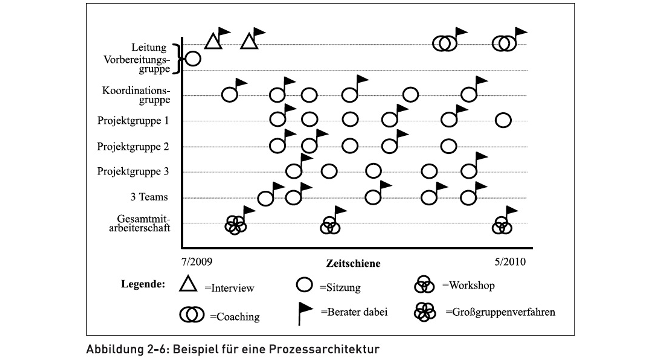
\includegraphics[keepaspectratio]{images/figure414.png}} \hfill{}

\caption{Abb. 4.14: Beispiel für eine Prozessarchitektur (Schiersmann \&
Thiel, 2014, S. 51)}

\end{figure}%

Es wird, wie in der Legende zu erkennen ist, zwischen unterschiedlichen
Formen der Arbeit im Rahmen der Organisationsentwicklung unterschieden.
Bspw. sind die Interviews als Dreiecke zu erkennen und die Sitzungen
sind als Kreis dargestellt. Es gibt außerdem unterschiedliche andere
Formen, wie zum Beispiel den Workshop im Großgruppenverfahren, wo die
gesamte Belegschaft der Einrichtung zusammenkommt und ein Berater dabei
ist. Wenn sich in der Grafik zwei Kreise überlappen, dann handelt es
sich um Coaching und andere Unterstützungsprozesse. Mit Hilfe der
Legende kann man diese Grafik gut lesen und es wird im Zeitablauf von
circa einem Jahr dargestellt, wo verschiedene Veränderungsmaßnahmen
umgesetzt worden sind. Wie links im Diagramm zu erkennen ist, lassen
sich die Beteiligten in verschiedene Gruppen unterteilen. Es gibt die
Leitung, die einbezogen wird und die ganz am Anfang in der ersten
Sitzung ausfindig machen muss, wo der Bedarf für den Veränderungsprozess
ist. Folglich wird mit den Beratern der Auftrag zum Veränderungsprozess
und die Methodik besprochen und gleichzeitig eine Koordinationsgruppe
einberufen. Trotzdem muss am Anfang (oder nachdem der Auftrag erklärt
worden ist) die gesamte Mitarbeiterschaft mit angesprochen und darüber
informiert werden, wo wir uns gerade in dem Prozess befinden. Über den
Prozessverlauf hin, also über die verschiedenen Monate die folgen, gibt
es sowohl auf Teamebene als auch auf Projektgruppenebene verschiedene
Ereignisse, die umgesetzt werden, wo nach Veränderungen geschaut und
entsprechend Lösungen entwickelt werden. Das geschieht hier auf Basis
der Projektarbeit in den verschiedenen Gruppen. Es sind Sitzungen,
welche teils mit einem Berater durchgeführt werden,
Großgruppenveranstaltungen und Workshops, die geplant sind und im
Veränderungsprozess stattfinden. Am Ende des Prozesses finden wir auf
der Leitungsebene verschiedene Coachingprozesse, die durchgeführt
werden, um die Leitung dabei zu unterstützen, Konsequenzen aus den
Erkenntnissen zu ziehen und die neuen Veränderungen verbindlich zu
machen. Die Leitung wird befähigt, Bericht gegenüber der Belegschaft zu
erstatten, was zukünftig verändert werden muss. Was wir auch erkennen
können ist, dass die Koordinationsgruppe -- das ist die zweite Ebene von
oben gesehen -- an ganz unterschiedlichen Stellen während des gesamten
Prozesses die Aufgabe hat, die verschiedenen Teams anzuleiten und
letztendlich auch die Ergebnisse der einzelnen Projektgruppen
zusammenzutragen, um diese dann zusammenzufassend der Leitung zu
übergeben bzw. mit der Leitung zu diskutieren.

Der hier dargestellte Prozess sieht relativ komplex aus, ist aber kein
extravagantes Beispiel und sehr stark an die Praxis angelehnt. Er zeigt
ganz deutlich, wie viele verschiedene Kommunikationspunkte und
Austauschbeziehungen es gibt und wie viele Sitzungen es geben muss, um
so einen Entwicklungsprozess sinnvoll ablaufen zu lassen. Dieses
Beispiel diente dazu, um uns einen Überblick zu verschaffen, wie man
solch einen Prozess gestalten kann, der partizipativ orientiert ist und
der stark auf die Arbeit in Projektgruppen ausgerichtet ist.

\subsection{Modelle der
Organisationsentwicklung}\label{modelle-der-organisationsentwicklung}

\subsubsection{Überblick}\label{uxfcberblick}

Nachdem wir von den Zielen und Formen sowie von den verschiedenen Ebenen
und dem Prozess von Organisationsentwicklung gesprochen haben, werden
wir uns nun verschiedene Ansätze, Konzepte und Modelle anschauen. Dazu
werden wir uns vorerst drei klassische Ansätze ansehen und einen
weiterführenden Ansatz besprechen.

Zunächst ist die~\emph{Feldtheorie von Kurt Lewin}~zu nennen. Darin geht
es um die Frage, wie man so etwas wie förderliche und nichtförderliche
Faktoren im Rahmen der Organisationsentwicklung unterscheiden,
herausfinden und entsprechend einsetzen kann.

Die~\emph{Aktionsforschung}~beschäftigt sich damit, wie wir forschen,
lernen und Praxisveränderungen gemeinsam entdecken können. Es ist
gewissermaßen ein Spiel zwischen Praxis und Theorie.

Das~\emph{Drei-Phasen-Modell von Kurt Lewin}~-- welches wir uns bereits
am Anfang des Semesters in den Grundlagen angeschaut haben -- beinhaltet
drei Phasen des Veränderungsprozesses, nämlich die Phasen Unfreezing --
Moving -- Refreezing.

Mit den neueren Modellansätzen, zu denen beispielsweise die lernende
Organisation gehört, werden wir uns im Rahmen der Organisationskultur
bzw. in den entsprechenden Seminaren beschäftigen. Letztendlich gibt es
verschiedene weitere Ansätze zu nennen, obwohl dieser einer der
bekanntesten ist.

Des Weiteren ist im Rahmen der Organisationsentwicklung der systemische
Ansatz relevant, bei dem es darum geht, die gesamte Einrichtung zu
betrachten. Dabei geht es nicht darum, einzelne Personen verantwortlich
und haftbar zu machen, dass Veränderungsprozesse umgesetzt werden,
sondern dass wir immer jede Veränderung aus der Perspektive der gesamten
Einrichtung denken müssen. Wenn Veränderung in einem Bereich
stattfindet, bedeutet dies, dass es auch Auswirkung auf einen anderen
Bereich hat. Das wäre ebenfalls beispielsweise einer der neueren
Ansätze. Darüber hinaus gibt es eine ganze Reihe von kundenspezifischen
Ansätzen, die sich in den letzten zwei, drei Jahrzehnten intensiv
entwickelt haben.

\subsubsection{Feldtheorie nach Kurt
Lewin}\label{feldtheorie-nach-kurt-lewin}

Beschäftigen wir uns nun mit dem ersten Modell der
Organisationsentwicklung, der Feld-Theorie nach Kurt Lewin. Kurt Lewin
war ein bekannter Psychologe im 20. Jahrhundert, der sich mit
verschiedenen Ansätzen beschäftigt hat, beispielsweise der Kraft- oder
Kräftefeld-Theorie. Was ist damit gemeint? Damit ist gemeint, dass
einerseits das Verhalten von uns Menschen als auch andererseits wir uns
als Person entwickeln und unsere Beziehung zur Umwelt durch verschiedene
Kräfte beeinflusst werden können, die positiv, aber auch negativ sein
können. Ein Beispiel für positive Kräfte wäre, wenn wir zum Beispiel
Hunger haben und das Bedürfnis verspüren, etwas zu uns zu nehmen. Wir
essen dann etwas (als Energielieferant) und erhalten durch diese
positive Kraft (durch Energiezufuhr) die Möglichkeit, unser Bedürfnis zu
befriedigen. Wenn man diese positive Kraft auf Organisationen überträgt,
dann geht es am Anfang darum, ein Problem zu analysieren und
herauszufinden, wo etwas stört bzw. wo etwas verändert werden muss, um
daraus dann Fragen ableiten zu können, wie beispielsweise: Was gibt es
für Faktoren, die den Veränderungsprozess unterstützen können? Das ist
in der Feld-Theorie im Rahmen der Organisationsentwicklung beschrieben.
Zusammengefasst bedeutet es, dass die menschliche Entwicklung in unserem
Handeln sowie die zwischenmenschlichen Beziehungen in der Gesamtheit ein
strukturiertes und dynamisches Feld darstellen. Durch verschiedene
Kräfte, die immer auf das eine und das andere wirken, kommt es zu
Veränderungen. Man kann sagen, das ganze Leben ist eine Veränderung.
Unsere gesamte menschliche Entwicklung ist Veränderung.

\begin{figure}

\pandocbounded{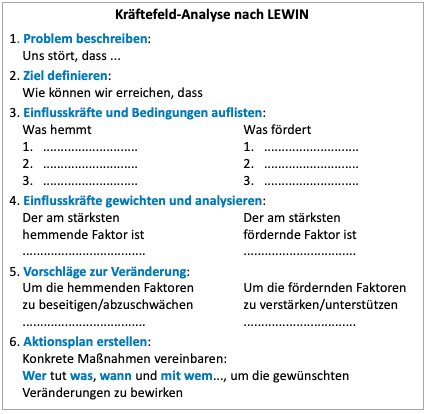
\includegraphics[keepaspectratio]{images/figure415.png}} \hfill{}

\caption{Abb. 4.15: Kräfte-Analyse von Lewin (nach Becker \& Langosch,
2002, zit n. Kolhoff, 2009, S. 23)}

\end{figure}%

In \hyperref[figure415]{Abb. 4.15} ist ein Kräftefeld dargestellt. Die
Kräftefeld-Analyse hat einen Stufenplan, den man durcharbeiten kann.
Dies ist hilfreich für die praktische Planung von
Organisationsentwicklungen. Am Anfang versucht man, das Problem zu iben.
Man erfasst, was stört bzw. was verändert werden muss und leitet daraus
seine Zielstellung ab. Was wollen wir erreichen? Was wollen wir
verändern? Dann kann man überlegen, welche Kräfte es gibt und welche
Rahmenbedingungen sich auf das Erreichen der Ziele auswirken -- entweder
hemmend oder fördernd. Wenn wir die Einflusskräfte -- positiv wie
negativ -- anschließend isoliert haben, können wir nun versuchen, diese
zu gewichten und zu priorisieren, was wie angegangen werden soll. Im
fünften Schritt machen wir uns nun Gedanken darüber, welche Maßnahmen
gegebenenfalls geeignet sind und welche Vorschläge es gibt, diese
Veränderung zu bewirken, beispielsweise wie hemmende Faktoren eventuell
beseitigt oder abgeschwächt werden können oder wie fördernde Faktoren
gestärkt und noch weiter unterstützt werden können. Daraus erstellen wir
als sechsten Schritt einen Aktionsplan, der über die Maßnahmen, die
Verantwortlichkeiten, den Zeitpunkt und die Teilziele informiert. Z. B.,
wer macht was, um die gewünschte Veränderung zu bewirken. Das ist ein
relativ einfaches, aber sehr praktikables Modell, um die
Organisationsentwicklung umzusetzen.

\subsubsection{Aktionsforschung}\label{aktionsforschung}

Im Rahmen der Aktionsforschung beeinflussen sich Veränderungen und das
Handeln der Betroffenen in einer Organisation gegenseitig. Die Forschung
dient dazu, das Handeln und die Betroffenen in Einrichtungen zu
unterstützen bzw. Anleitung zu geben, wie der Veränderungsprozess
bewältigt werden kann. Dabei werden unterschiedliche Rollen eingenommen
-- wie die Forscher*innen, die jeweils agierenden Betroffenen der
Einrichtungen und die Personen, die den Prozess beobachten -- weil
einerseits die Forschenden gleichzeitig auch als Praktiker unterwegs
sind und Dinge innerhalb der Organisation verändern und Aktionen
umsetzen und andererseits auch die Beteiligten in Organisationen den
Prozess mit erforschen, indem sie reflektieren, was die Veränderung ist
und welche Veränderungen bewirkt werden sollen. Wir können davon
ausgehen, dass dabei verschiedene Prozesse parallel stattfinden, also
Forschen in dem Sinne, dass wir versuchen herauszufinden, wie die
aktuelle Situation ist. Erst dann können wir die Situation verändern, in
dem wir Ziele setzen. Kurz zusammengefasst heißt das: Auf Basis dieser
Forschung kommt es zu Veränderungen in der Praxis, die letztendlich zu
Verbesserungen führen sollen, nämlich wie wir lernen, wie die
Organisationen sich weiterentwickeln können, wie wir Innovationen
umsetzen und wie das letztendlich wieder der Ausgangspunkt für einen
erneuten Start dieses Prozesses sein kann (vgl.
\hyperref[figure416ux5cux255D]{Abb. 4.16}).

\begin{figure}

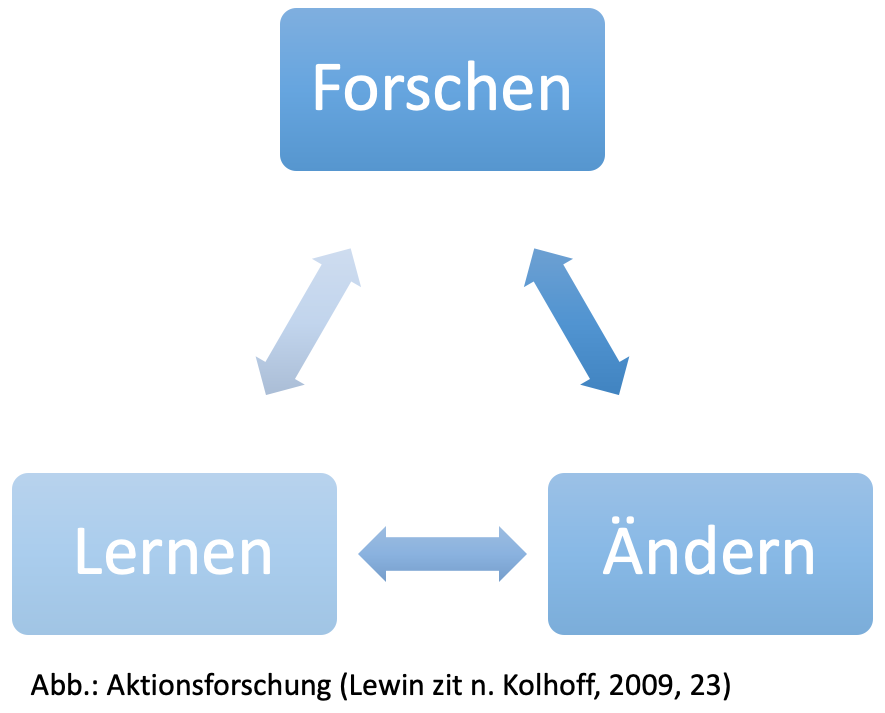
\includegraphics[width=0.6\linewidth,height=\textheight,keepaspectratio]{images/figure416.png} \hfill{}

\caption{Abb. 4.16: Aktionsforschung (nach Lewin zit n. Kolhoff, 2009,
S. 23)}

\end{figure}%

Das Dreieck symbolisiert einen Kreislauf. Forschung ist Ausgangspunkt,
wurde selbst zum Forschungsgegenstand und kann hinterfragt werden: (1)
Haben wir die Ziele erreicht und (2) was muss vielleicht zukünftig noch
entwickelt werden, weil sich beispielsweise die Rahmenbedingungen schon
wieder geändert haben? Das Modell zeigt, dass sich die forschende
Haltung, die Änderungshaltung und das kontinuierliche Lernen beständig
abwechseln. Dabei handelt es sich um ein theoretisches Modell, welches
einfach in der Praxis umgesetzt werden kann. Im Rahmen einer
Abschlussarbeit über einen Veränderungsprozess innerhalb einer
Einrichtung können wir dokumentieren und retrospektiv herausfinden, wie
umgesetzt wurde. Daraus können wir ein Konzept entwickeln und gehen mit
diesem in die Einrichtung. In der Einrichtung finden wir die
Mitwirkenden vor, die den Änderungsprozess umsetzen, die das Feld ändern
und gleichzeitig in der Organisation lernen. In einer anschließenden
Evaluation oder Reflexion können die Mitwirkenden ausfindig machen, was
innerhalb der Einrichtung zu einer Veränderung geführt hat bzw. welche
Faktoren sich in der Einrichtung verändert haben. Im weiteren Sinne
handelt es sich hierbei um eine Handlungsforschung, die wir mit unserer
Abschlussarbeit betreiben würden, da wir ein Konzept entwickeln, dieses
Konzept umsetzen und hinterher überprüfen, ob dieses tatsächlich
sinnvoll umgesetzt werden konnte.

\subsubsection{Dreiphasen-Modell der Organisationsentwicklung nach Kurt
Lewin}\label{dreiphasen-modell-der-organisationsentwicklung-nach-kurt-lewin}

Im~\emph{Drei-Phasen-Modell von Kurt Lewin}~werden drei
Entwicklungsphasen unterschieden (vgl. \hyperref[figure417]{Abb. 4.17}).

\begin{figure}

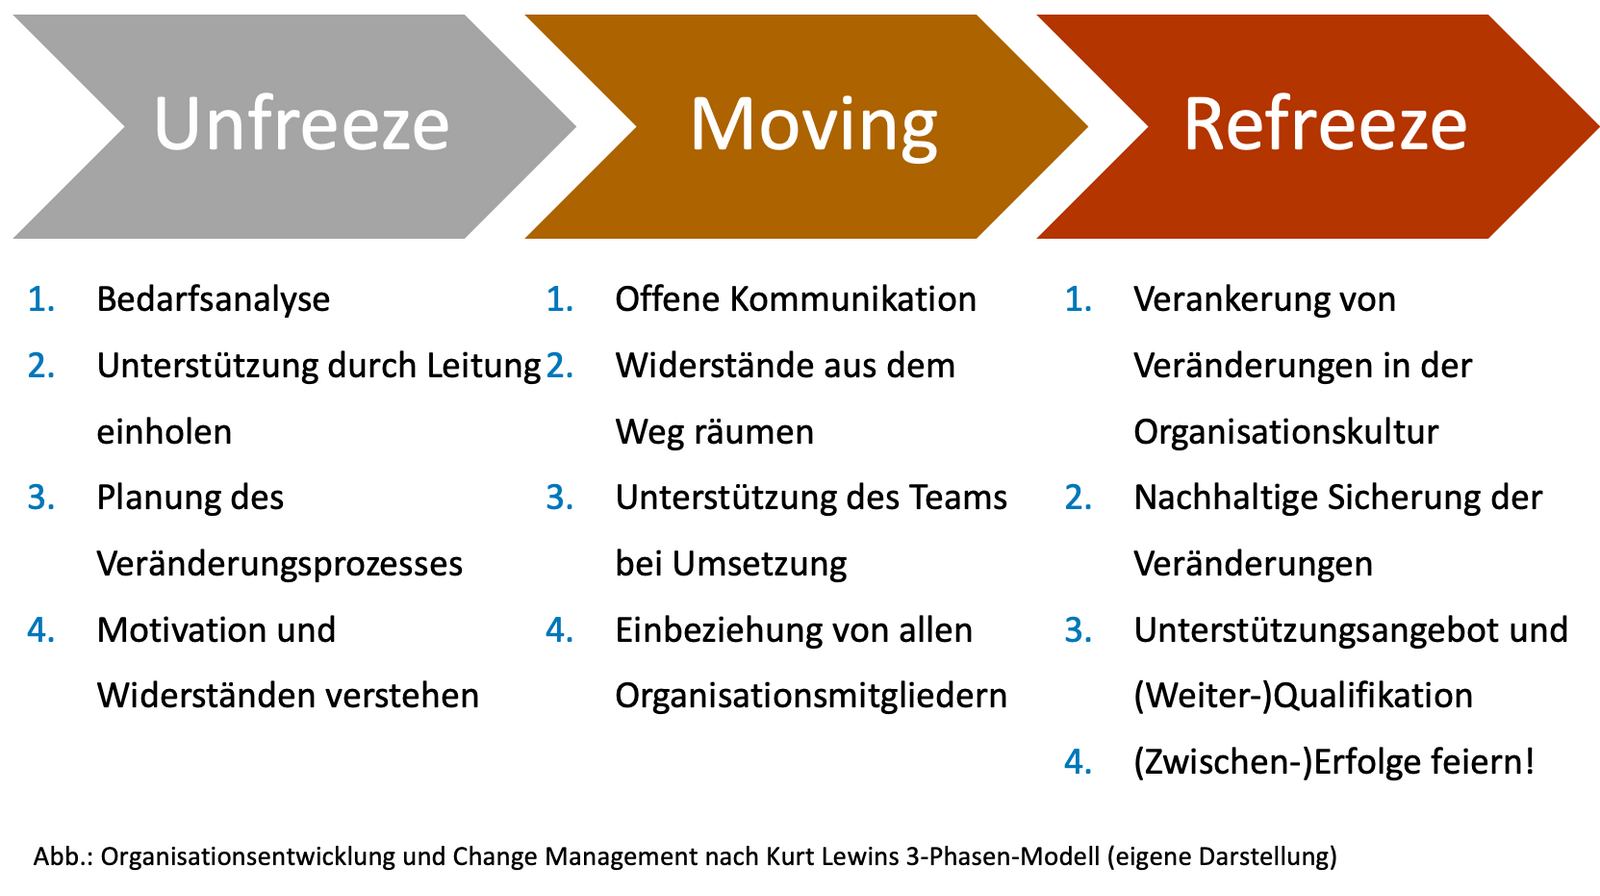
\includegraphics[width=0.8\linewidth,height=\textheight,keepaspectratio]{images/figure417.png} \hfill{}

\caption{Abb. 4.17: Organisationsentwicklung und Change-Management nach
Kurt Lewins 3-Phasen-Modell (eigene Darstellung)}

\end{figure}%

Kurz zur Begrifflichkeit: Beim~\emph{Unfreezing}~(1. Phase) geht es
darum, die bisherigen Strukturen zu analysieren und in Frage zu stellen.
Dabei geht es darum, Veränderungen umzusetzen, Maßnahmen dafür zu
ergreifen und Aktionen zu planen.~\emph{Refreezing}~(2. Phase) bedeutet
in diesem Modell „etwas verbindlich machen'' oder „einfrieren''. Dabei
erfolgt das „Einfrieren'' der neu gefundenen Strukturen, Prozesse und
Abläufe, mit anderen Worten eine Verbindlichmachung und Legitimation der
Veränderungen.

Im~\emph{Unfreezing}~(1. Phase) geht es auch darum, den Bedarf zu
ermitteln. Durch die Einrichtungsleitung muss auch Unterstützung
eingeholt werden, weil Veränderungsprozesse grundsätzlich einfach dann
gut funktionieren, wenn die Leitung dahintersteht und über sie die
Veränderung gegebenenfalls eingefordert werden kann. Des Weiteren muss
der Veränderungsprozess vorbereitet werden, die Methodik muss
abgesprochen werden, der Zeitraum sowie die dafür zur Verfügung
stehenden Ressourcen (Personalressourcen und Sachressourcen) müssen
geplant werden und schließlich geht es darum, über die Veränderungen
erst einmal zu informieren und bei Widerständen bzw. bei auftretenden
Fragen entsprechend zu motivieren und den Veränderungsprozess
verständlich zu machen und zu erklären, warum wir uns in diese
Veränderung hinein begeben werden.

Beim~\emph{Moving}~(2. Phase) geht es schließlich darum, Aktionen und
Maßnahmen zu planen, um dann die Veränderung zu bewirken. Hier gilt es
Prinzipien einzuhalten, wie z. B., dass offen kommuniziert wird, dass
regelmäßig informiert wird und dass alle an dem Vorhaben beteiligt
werden. Es gilt, aktiv zu kommunizieren, Widerstände zu bearbeiten und
aus dem Weg zu räumen. Meistens lassen sich nicht alle Widerstände aus
dem Weg räumen und man muss versuchen, möglichst alle im Team bzw. in
der Einrichtung anzusprechen und zu beteiligen, damit der
Veränderungsprozess erfolgreich umgesetzt werden kann. Wir müssen die
Unterstützung im Team suchen bzw. -- und das haben wir vorhin bei der
Prozessbeschreibung von Organisationsentwicklung schon gesehen --
einzelne Projektgruppen oder Teams mit Aufgabenstellungen betrauen, um
hierfür dann Lösungen zu suchen. Darüber hinaus geht es darum,
Organisationsmitglieder einzubeziehen und Partizipation zu erleben.

Im abschließenden~\emph{Unfreezing}~(3. Phase) geht es um das
Verbindlichmachen der neu gefundenen Strukturen, Prozesse und
kulturellen Überzeugungen. Es geht darum, diese zu verankern und
maßgeblich die Organisationskultur weiterzuentwickeln. Hier geht die
Organisationsentwicklung mit der Entwicklung der Organisationskultur
einher (vgl. Abschnitt 2.4). Wichtig ist auch die nachhaltige Sicherung
der Veränderung, dass man die Dinge, die man verändern hat, festschreibt
bzw. gegebenenfalls eine Dienstvereinbarung daraus entwickelt und als
den neuen „Status quo'' festgelegt. Es werden auch
Unterstützungsnotwendigkeiten angesprochen, bspw. für eine
Weiterqualifikation, um damit weiterarbeiten zu können. Zum Schluss
schließlich sollte jede einzelne Phase, jeder einzelne Prozessschritt
auch gefeiert werden. Diesen dreiphasigen Prozess kann man auch als eine
Art Kreislaufsystem betrachten, der immer wieder abläuft und der sich in
verschiedenen Phasen auch fortentwickelt.

\subsubsection{Fazit}\label{fazit}

Die drei vorgestellten klassischen Modelle kann man wie folgt
zusammenfassen: Es gibt im Regelfall drei Phasen, die im Rahmen der
Organisationsentwicklung mitbedacht werden sollen. Am Anfang steht die
Phase der~\emph{Diagnose}. In dieser verschaffen wir uns einen Überblick
über den Ist-Stand. In der zweiten Phase versuchen wir,~\emph{Maßnahmen
der Veränderung umzusetzen}~und dementsprechend auch einen neuen „Status
quo'' zu erreichen. Und schließlich -- drittens -- ist es die Aufgabe
der Leitung bzw. aller Einrichtungsmitglieder und Führungskräfte dafür
zu sorgen, dass die neu gefundenen Aufgaben, Prozesse, Strukturen
entsprechend umgesetzt werden bzw. zukünftig als~\emph{verbindlich
legitimiert} werden.

\chapter{Finanzierung in der
Sozialwirtschaft}\label{finanzierung-sozialwirtschaft}

Im Rahmen der Finanzplanung muss dargestellt werden, wie die für den
Geschäftsbetrieb benötigten finanziellen~Mittel beschafft und verwendet
werden sowie wann und in welcher Höhe mit einem Ab- und Zufluss~der
benötigten Mittel zu rechnen ist. Für das Verständnis der verschiedenen
Zahlen und Zusammenhänge~sind die folgenden drei Grundbegriffe zu
beachten:

\begin{itemize}
\item
  \emph{Liquidität} beschreibt die Zahlungsfähigkeit, also die
  Fähigkeit, jederzeit den Zahlungsverpflichtungen uneingeschränkt
  nachkommen zu können. Ziel eines jeden Unternehmen ist es,
  kontinuierlich einen positiven Bestand an finanziellen Mitteln zu
  verwalten.
\item
  \emph{Finanzierung} (i. e. S.) meint die Fähigkeit, für den
  kurzfristigen bzw. längerfristigen Geschäftsbetrieb ausreichend
  finanzielle Mittel zur Verfügung zu stellen.
\item
  \emph{Wirtschaftlichkeit} beschreibt den Zusammenhang aus
  erforderlichem Aufwand und erreichtem Erfolg. Ein Unternehmen ist
  besonders dann wirtschaftlich, wenn die eingesetzten Mittel effektiv
  zur Zielerreichung eingesetzt wurden und die getätigten Investitionen
  rentabel sind.
\end{itemize}

Zwar steht bei der Finanzierung als Teil des betrieblichen
Rechnungswesens nur die Planung, Kontrolle und Steuerung von
Zahlungsströmen (Liquiditätsrechnung, Kapitalbedarfsplanung,
Cashflowrechnung,~ Investitionsplanung) im Mittelpunkt, die zur
Umsetzung des operativen Tagesgeschäftes und für eine strategisch
Unternehmensentwicklung notwendig sind, es müssen darüber hinaus aber
noch weitere betriebliche Rechnungen (externes Rechnungswesen)
einbezogen werden, wie z. B. die Darstellung der Vermögens- und
Schuldenlage in Form der Planbilanz und der Erfolgsaussichten in Form
der Plan- Gewinn-und-Verlustrechnung.

Der Finanzplanung muss besondere Aufmerksamkeit geschenkt werden, da
diese von Investoren genau geprüft und hinsichtlich der finanziellen
Machbarkeit der Gründung, möglicher Finanzrisiken, Maßnahmen zur
Kapitalbeschaffung und notwendiger Investitionen geprüft wird.

Im Folgenden werden die Grundlagen der Finanzierung von Organisationen
der Sozialwirtschaft beschrieben. Ausgehend vom Welfare-Mix werden
hernach die betriebswirtschaftlichen und schließlich
sozialwirtschaftlichen Finanzierungsformen dargestellt.

\section{Welfare-Mix in der
Sozialwirtschaft}\label{welfare-mix-sozialwirtschaft}

Wie im \hyperref[gesamtwirtschaft]{Gesamtwirtschaftliche Einordnung der
Sozialwirtschaft} bereits erläutert wurde, müssen sich Sozialunternehmen
bzw. freie Träge der Wohlfahrtspflege heutzutage aufgrund der besonderen
rechtlichen, wirtschaftlichen und organisationalen Rahmenbedingungen in
der Sozialwirtschaft aus unterschiedlichen Quellen finanzieren. Die
Zeiten der vollumfänglichen Finanzierung nach dem Kostendeckungsprinzip
durch die öffentliche Hand sind schon seit geraumer Zeit vorbei. Daher
müssen Träger neben Finanzmitteln der öffentlichen Hand (z. B.
Zuwendungen, Zuschüsse) auch Beiträge von Privatpersonen oder
Unternehmen sowie finanzielle Mittel, die aus Fundraisingaktivitäten (z.
B. Spenden, Sponsoring, Crowdfunding) stammen, erwirtschaften. Nicht zu
vergessen sind dabei aber auch die verschiedenen
betriebswirtschaftlichen Finanzierungsmöglichkeiten der Selbst- bzw.
Eigenfinanzierung (wie z. B. Eigenmittel, die aus Gewinnen
erwirtschaftet wurden, Abschreibungen für Abnutzung von
Anlagegegenständen, Rücklagenbildung). Als Beispiel sei auf den
Finanzierungsmix des Deutschen Caritasverbands e. V. verwiesen, welcher
in der Infographik in \hyperref[figure51]{Abb. 5.1} in Form
unterschiedlicher Finanzierungsquellen dargestellt wird. Im Rahmen der
Existenzgründung ist daher die Suche nach unterschiedlichen
Finanzierungsquellen gleich von Anfang an mitzudenken und entsprechend
in die Finanzplanung einzubeziehen.

\begin{figure}

\pandocbounded{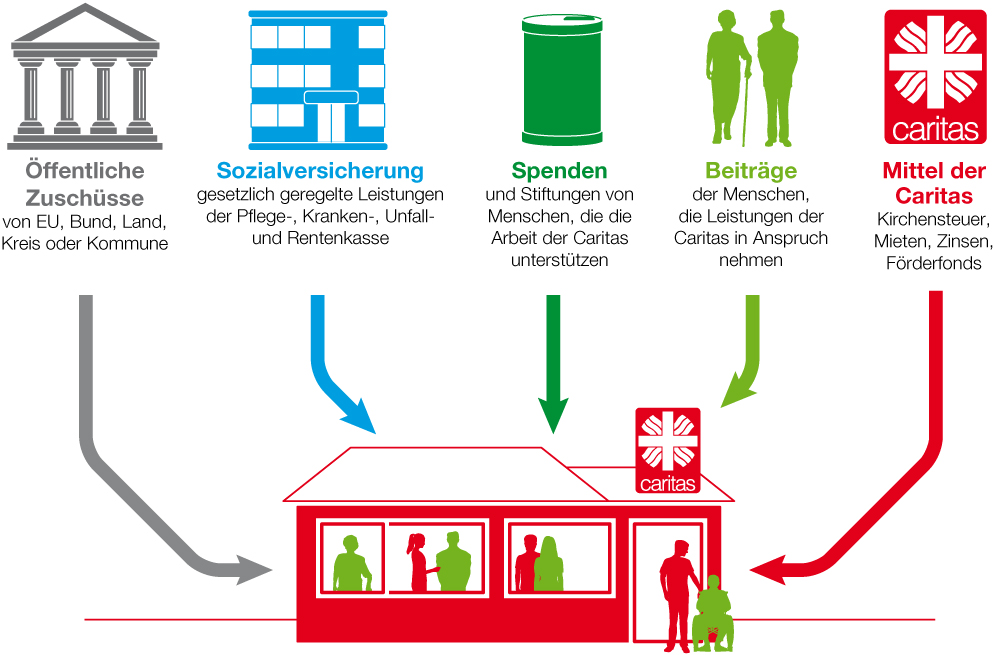
\includegraphics[keepaspectratio]{images/figure51.jpeg}} \hfill{}

\caption{Abb. 5.1: Finanzierungsmix (Deutscher Caritasverband e.V.,
2025, S. 3)}

\end{figure}%

Im Beispiel gesprochen heißt das: Leistungen des Deutscher
Caritasverband e.V. (2025) werden über folgende Quellen finanziert:

\begin{itemize}
\item
  \emph{Leistungsentgelte} der Leistungsträger (Sozialversicherungen)
  für z. B. Krankenhäuser, Sozialstationen, Pflegeeinrichtungen;
\item
  \emph{Eigenbeiträge} der Leistungsempfänger (Selbstzahlerbeiträge) z.
  B. für Leistungen in der Kindertagespflege, Sozialstation,
  Pflegeeinrichtung;
\item
  \emph{Zuschüsse} von Bund, Ländern und Kommunen für die Finanzierung
  von Aufgaben und Leistungen in Kindertagesstätten, Wohnheimen für
  Menschen mit Behinderung, Beratungsstellen;
\item
  \emph{Eigenmittel} (z. B. Erträge aus Vermögen, Vermietung und
  Verpachtung, Kirchensteuern, Kirchenkollekten sowie Zuschüssen von
  Soziallotterien und Förderstiftungen) dienen meist dazu, Pilot- und
  Modellprojekte zu realisieren oder auch Menschen in besonderen
  Lebenslagen zu unterstützen, wenn keine andere soziale, rechtliche und
  wirtschaftliche Absicherung gegeben ist.
\item
  \emph{Spenden, Beiträge und Stiftungsmittel} unterstützen allgemein
  die Arbeit des Caritasverbands und werden für festgelegte Zwecke
  eingesetzt.
\end{itemize}

Auf die unterschiedlichen Finanzierungsquellen gilt es nun noch einmal
näher einzugehen.

\section{Betriebswirtschaftliche
Finanzierungsformen}\label{betriebswirtschaftliche-finanzierungsformen}

\subsection{Grundbegriffe}\label{grundbegriffe-finanzierungsformen}

Im Rahmen der Finanzierung einer Unternehmung kann aus
betriebswirtschaftlicher Sicht auf unterschiedliche Typen von
finanziellen Mitteln bzw. Kapitalsorten zurückgegriffen werden. Man
unterscheidet dabei allgemein zwischen den Formen einer Innen- und
Außenfinanzierung (Frage nach der Herkunft der Mittel) sowie einer
Eigen- und Fremdfinanzierung (Frage nach Kapitalsorten und Art der
Kapitalüberlassung). Zur \emph{Innenfinanzierung} gehören alle Maßnahmen
der Kapitalbeschaffung aus der eigenen Unternehmung (z. B. aus der
Umsatztätigkeit oder durch Vermögensumschichtungen). Demgegenüber wird
bei der \emph{Außenfinanzierung} Fremdkapital vom Kapitalmarkt bzw. von
anderen Unternehmen akquiriert (z. B. durch Kapitaleinlagen von
Gesellschaftern, Kredite). Bei der \emph{Eigenfinanzierung} steht die
Gewinnung von zusätzlichem Eigenkapitel (mit erfolgsabhängigen Zahlungen
wie Ausschüttungen, Dividenden etc.) im Vordergrund. Die
\emph{Fremdfinanzierung} zielt auf die Beschaffung von Fremdkapitel (mit
erfolgsunabhängigen Zins- und Tilgungsverpflichtungen), z. B. Kredite,
Kontokorrent, Lieferantenkredit). Wie an diesen Begrifflichkeiten zu
bemerken ist, gibt es verschiedene Überschneidungen in den
Begrifflichkeiten. Diese sind in der folgenden \hyperref[figure52]{Abb.
5.2} dargestellt und werden im Folgenden näher erläutert (Heister,
2016).

\begin{figure}

\pandocbounded{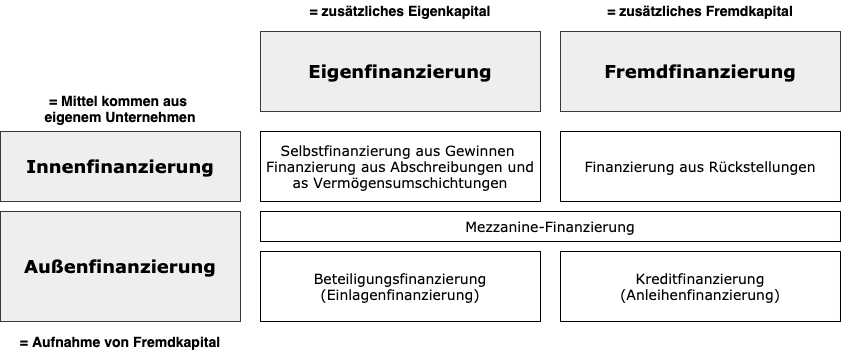
\includegraphics[keepaspectratio]{images/figure52.png}} \hfill{}

\caption{Abb. 5.2: Typologie betriebswirtschaftliche Finanzierungsformen
(Heister, 2016, S. 24)}

\end{figure}%

\subsection{Innenfinanzierung}\label{innenfinanzierung}

Maßnahmen der Innenfinanzierung können auf die Beschaffung von
Eigenkapitel durch z. B. die Selbstfinanzierung aus einbehaltenen
Überschüssen im Rahmen der Gewinnermittlung (= offene Selbstfinanzierung
bzw. Gewinnthesaurierung), die Finanzierung aus Abschreibungen und die
Vermögensumschichtung (= Kapitalfreisetzung in Folge von Einsparungen,
Verkauf von Anlagevermögen und Saleand- Lease-Back-Maßnahmen) gerichtet
sein. Weiterhin kann die Innenfinanzierung auch auf die
Fremdkapitalbildung Auswirkung haben, z. B. im Rahmen der kaufmännischen
Jahresabschlusserstellung durch Bildung von Rückstellungen nach § 249
HGB für ungewisse Verbindlichkeiten von Dritten und die Ausübung von
Wahlrechten im Rahmen der Bilanzierung (= stille Selbstfinanzierung, z.
B. Überbewertung von Aktiva/Vermögen, Unterbewertung von
Passiva/Schulden, Nichtaktivierung aktivierungsfähiger Wirtschaftsgüter,
Unterlassung der Zuschreibung bei Wertsteigerungen z. B. wenn ein
Gebäude niedriger bewertet wird als der entsprechende Marktwert).

Auf die beiden Finanzierungsmöglichkeiten Abschreibungen und
Rückstellungen ist noch einmal näher einzugehen, da dies Auswirkung auf
die Entwicklung des Cashflows (Zahlungsmittelbestands) haben kann:

\begin{enumerate}
\def\labelenumi{\arabic{enumi}.}
\tightlist
\item
  \emph{Abschreibungen} auf die Abnutzung von Gegenständen des
  Anlagenvermögens vermindern im Rahmen der Gewinn- und Verlustrechnung
  den Gewinn (vgl. im Folgenden Kolhoff \& Bettig, 2013). Es fließen dem
  Unternehmen keine neuen Gelder zu, sondern Abschreibungen können in
  der Finanzbuchhaltung als Aufwendungen geltend gemacht werden.
  Erfasste Abschreibungen sollen im Rahmen von Kalkulationen für
  Projekte, Vergabe von Fördermitteln oder bei Dienstleistungen, die
  durch Eigenbeiträge der Klienten*innen getragen werden (Selbstzahler)
  berücksichtigt werden und generieren damit zukünftige Zahlungsströme
  (= Anteile des erhaltenen Umsatzes). Über die Umsätze können
  Abschreibungen gewissermaßen „(zurück)verdient'' werden. Damit können
  Ersatzinvestitionen (z. B. Neuanschaffung von abgeschriebenen
  Fahrzeugen) getätigt werden. Zusätzlich ergibt sich aber noch ein
  anderer Vorteil: Abschreibungen vermindern die Steuerlast (vgl. dazu
  \hyperref[figure53]{Abb. 5.3}).
\end{enumerate}

\begin{figure}

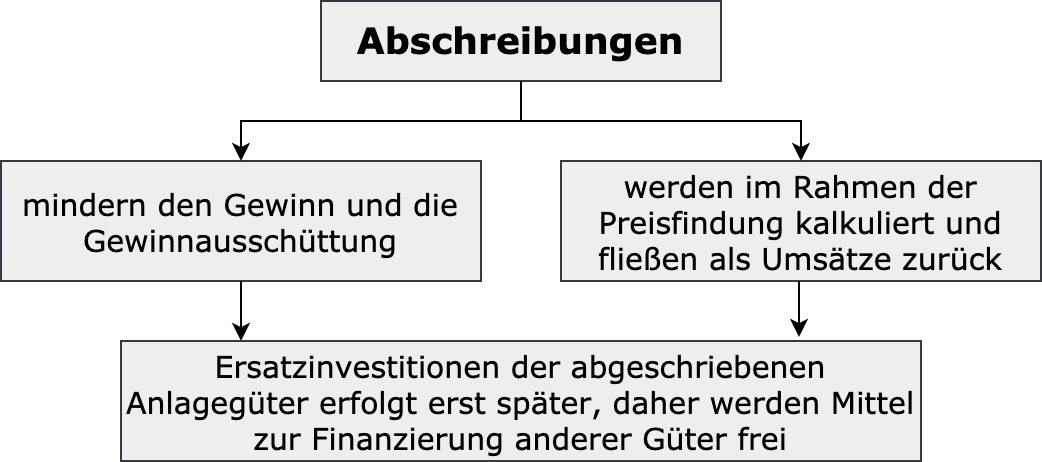
\includegraphics[width=0.7\linewidth,height=\textheight,keepaspectratio]{images/figure53.png} \hfill{}

\caption{Abb. 5.3: Finanzierung aus Abschreibungen (Kolhoff \& Bettig,
2013, S. 68)}

\end{figure}%

\emph{Rückstellungen} stellen Verbindlichkeiten gegenüber Dritten dar,
deren Eintritt, Höhe und/ oder Fälligkeit als unsicher gelten (§ 249
HGB) wie z. B. bei Pensionszahlungen, Steuerrückstellungen,
Instandsetzungsmaßnahmen, Prozesskosten für schwelende
Gerichtsverfahren. Rückstellungen müssen im Rahmen der
Jahresabschlusserstellung gebildet und wieder aufgelöst werden, wenn
deren Grund weggefallen ist. Rückstellungen sind ein Beispiel für das
kaufmännische Vorsichtsprinzip im Rahmen des externen Rechnungswesens.
Sie haben eine ähnliche Wirkung wie Abschreibungen. Bei
Rückstellungsbildung wird ein Teil des Gewinnes einbehalten. Dies führt
nicht sofort zu Auszahlungen, sondern entsprechende Ansätze müssen im
Rahmen der Kalkulation von Aufträgen erfasst werden und fließen damit zu
einem späteren Zeitpunkt als Umsätze wieder zurück. Bei Auflösung von
Rückstellungen im Rahmen der Bilanzierung entsteht ein höherer Gewinn
(vgl. \hyperref[figure54]{Abb. 5.4}).

\begin{figure}

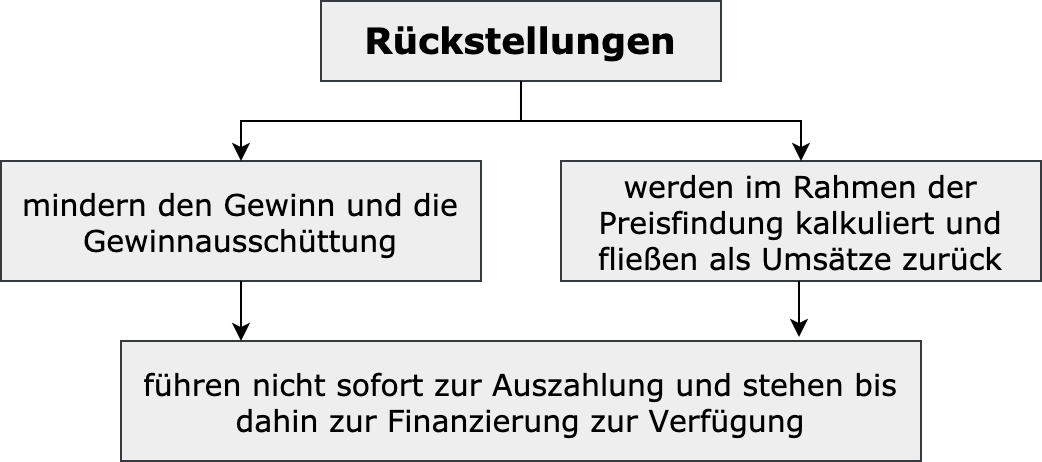
\includegraphics[width=0.7\linewidth,height=\textheight,keepaspectratio]{images/figure54.png} \hfill{}

\caption{Abb. 5.4: Finanzierung aus Rückstellungen nach § 249 HGB
(Kolhoff \& Bettig, 2013, S. 69)}

\end{figure}%

\subsection{Außenfinanzierung}\label{aussenfinanzierung}

Bei der Außenfinanzierung kann durch zusätzliche Kapitaleinlagen von
bestehenden Gesellschaftern oder durch Dritte (Beteiligungsfinanzierung)
Eigenkapitel aufgebaut werden. Darüber hinaus ermöglichen bei der
Außenfinanzierung die Kreditaufnahme oder die Herausgabe einer Anleihe
eine Beschaffung von Fremdkapitel, also Schulden und Verbindlichkeiten,
die über eine bestimmte Laufzeit getilgt und verzinst werden. Von einer
Mezzanine-Finanzierung (ital., \emph{mezzanine} für
Halb-/Zwischengeschoss) spricht man immer dann, wenn die
Kapitalbeschaffung hinsichtlich ihrer rechtlichen und wirtschaftlichen
Ausgestaltung eine Mischform zwischen Eigen- und Fremdkapital darstellt
(z. B. Gesellschafterdarlehen, stille Beteiligungen,
Wandel-/Optionsanleihen, Genussscheine). Im Rahmen der
Außenfinanzierung, die gleichzeitig auch Fremdfinanzierungen sind,
können neben der bereits erwähnten Kreditaufnahme, Ausgabe von Anleihen
und dem Lieferantenkredit außerdem noch andere -- in der
\hyperref[table51]{Tab. 1} dargestellte -- Finanzierungsmöglichkeiten
genutzt werden.

\begin{longtable}[]{@{}
  >{\raggedright\arraybackslash}p{(\linewidth - 2\tabcolsep) * \real{0.5000}}
  >{\raggedright\arraybackslash}p{(\linewidth - 2\tabcolsep) * \real{0.5000}}@{}}
\caption{Tab. 5.1: Formen der Fremdkapitalfinanzierung (Schellberg,
2004, S. 188; zit. n. Kolhoff \& Bettig, 2013, S. 70-71)}\tabularnewline
\toprule\noalign{}
\begin{minipage}[b]{\linewidth}\raggedright
\textbf{Finanzierung}
\end{minipage} & \begin{minipage}[b]{\linewidth}\raggedright
\textbf{Beschreibung}
\end{minipage} \\
\midrule\noalign{}
\endfirsthead
\toprule\noalign{}
\begin{minipage}[b]{\linewidth}\raggedright
\textbf{Finanzierung}
\end{minipage} & \begin{minipage}[b]{\linewidth}\raggedright
\textbf{Beschreibung}
\end{minipage} \\
\midrule\noalign{}
\endhead
\bottomrule\noalign{}
\endlastfoot
Kontokorrentkredit & Unbürokratischste Form des Kredits. Das Konto der
Einrichtung kann gegen Zinszahlung im Rahmen der Kreditlinie überzogen
werden. \\
Hypothekenkredit & Langfristiger Kredit gegen Sicherheit einer
Immobilie, i.d.R. durch Eintragung einer Grundschuld. \\
Lieferantenkredit & Mit Erhalt der Ware wird ein Zahlungsziel
vereinbart. Bis zum Zahlungsziel steht das Geld für Investitionen zur
Verfügung. \\
Anzahlungen von Kunden & Stellen einen kurzfristigen Kredit der Kunden
dar. \\
Bürgschaftskredite & Ein Dritter - der Bürge - tritt als Schuldner ein,
falls der eigentliche Schuldner nicht mehr bezahlen kann, häufig in Form
einer Patronatserklärung. \\
Anleihen & Kredit, der in Teilbeträgen gestückelt wird und als Anleihe
an Kreditgeber gegeben wird. \\
\end{longtable}

Es ist nicht immer leicht, im Rahmen der Finanzplanung den richtigen Mix
aus verschiedenen Finanzierungen zu wählen. Folgende Kriterien können
bei der Wahl von Finanzierungsquellen hilfreich sein (Kolhoff \& Bettig,
2013, S. 70-71): Im Falle einer Kapitaleinlage (Aufnahme von
Eigenkapital) werden die Stimm- und Mitspracherechte
(Entscheidungsbefugnisse) berührt und eine Erfolgsbeteiligung der neuen
Gesellschafter notwendig, während im Falle der Aufnahme von Fremdkapital
in der Regel keine Mitspracherechte wie z. B. der Bank bei
Kreditaufnahme zu befürchten sind. Im Falle eines Kredits sind über eine
definierte Laufzeit Zins- und Tilgungsraten als Entgelte zu zahlen. Die
Zinszahlungen können wiederum als Aufwendungen geltend gemacht werden
und führen zu einer Verminderung der Steuerlast. Hinsichtlich der
Verfügbarkeit steht Eigenkapital in der Regel über unbegrenzte Zeit zur
Verfügung, während Fremdkapitel grundsätzlich nur zeitlich befristet
genutzt werden kann.

\section{Finanzierungsformen in der
Sozialwirtschaft}\label{finanzierungsformen}

\subsection{Grundbegriffe}\label{grundbegriffe-finanzierungsformen-sozialwirtschaft}

Neben den eben dargestellten betriebswirtschaftlichen
Finanzierungsmöglichkeiten haben Sozialunternehmen darüber hinaus Zugang
zu bestimmten sozialwirtschaftlichen Finanzierungen. Man unterscheidet
dabei zwischen einer öffentlichen und nicht-öffentlichen Finanzierung.
Zur öffentlichen Finanzierung zählen insbesondere die Subjekt- und
Objektfinanzierung, die zur Kostendeckung der angebotenen
personenbezogenen sozialen Dienstleistungen zunächst herangezogen werden
können. Bei der \emph{Subjektfinanzierung} handelt es sich um eine
sogenannte indirekte Finanzierung, da -- im Sinne des sozialrechtlichen
Dreiecks -- der Leistungserbringer die für die Kostendeckung notwendigen
Finanzmittel nicht vom Leistungsempfänger, sondern (indirekt) vom
Leistungsträger entschädigt bekommt (z. B. Leistungsentgelte,
persönliches Budget, Gutscheine). Im Rahmen einer
\emph{Objektfinanzierung} erhält ein sozialer Träger Zuwendungen bzw.
Zuschüsse der öffentlichen Hand wie z. B. Kommune, Land oder Bund.

Die Subjektfinanzierung (auch indirekte Finanzierung) findet im Rahmen
des bereits in Abschnitt 3.1 erwähnten sozialrechtlichen
Dreiecksverhältnisses zwischen Leistungsempfänger, Leistungsanbieter und
Leistungsträger statt. Dabei findet eine Finanzierung über die
„Konsumenten'' sozialer Dienstleistungen statt, z. B. in Form von
Leistungsentgelten, persönlichem Budget oder Gutscheinen.
Anspruchsberechtigt sind nicht freie Träger an sich, sondern
Klienten*innen (z. B. in Form von services in cash oder services in
kind). Unter einer Objektfinanzierung (auch direkte Finanzierung)
versteht man die Förderung von Leistungen, Projekten oder bestimmter
öffentlicher Aufträge (z. B. Einrichtung von Beratungsstellen) in Form
von Zuwendungen, Zuschüssen oder Subventionen durch die öffentliche Hand
(Kolhoff, 2017, S. 4). Zur nicht-öffentlichen Finanzierung zählen
insbesondere Zuwendungen von Stiftungen, Kirchen oder anderen
Körperschaften des öffentlichen Rechts, Spenden von Privatpersonen oder
Unternehmen, Vereinsbeiträge, Einnahmen aus Fundraisingaktivitäten
(Kolhoff \& Bettig, 2013, S. 23). Die genannten sozialwirtschaftlichen
Finanzierungsformen werden im Folgenden noch einmal ausführlicher
vorgestellt.

\subsection{Subjektfinanzierung}\label{subjektfinanzierung}

Neben der Finanzierung von \emph{Leistungsentgelten} im Rahmen des
Dreiecksverhältnisses der Leistungserbringung haben sich in jüngster
Zeit noch andere Möglichkeiten der Subjektfinanzierung entwickelt, die
als \emph{Einkaufsmodell} funktionieren. Bei dieser Finanzierungsform
können Leistungsberechtigte „statt einer Sach- eine Geldleistung wählen,
mit der sie soziale Dienstleistungen am Sozialmarkt frei einkaufen
können'' (Kolhoff, 2017, S. 4). Als Sonderform des Einkaufsmodells hat
sich auch der Einsatz von \emph{Gutscheinen} bewährt, wie sie „z. B. für
Maßnahmen der Aktivierung und beruflichen Eingliederung, die berufliche
Weiterbildung und für Bildungs- und Teilhabeleistungen für bedürftige
Schülerinnen und Schüler ausgegeben'' werden und auch im Bereich von
Kindertagesstätten (Kolhoff, 2017, S. 9).

\subsection{Leistungsentgelte}\label{leistungsentgelte}

\emph{Leistungsentgelte} stellen monetäre Vergütungen dar, die auf
vertraglicher Basis vom Leistungsträger an den Leistungserbringer zur
Deckung der Kosten bei Inanspruchnahme von Leistungen durch
anspruchsberechtigte Personen entstehen. Leistungsentgelte müssen im
Rahmen von Leistungsvereinbarungen entweder direkt zwischen Kostenträger
(Jugendamt, Sozialversicherung) und Leistungserbringer (z. B. Kita,
Pflegeheim) oder indirekt zwischen Kostenträger und Verbänden der freien
Jugendhilfe (§ 78 SGB VIII; Landesrahmenverträge) verhandelt werden.
Inhalt der Leistungsvereinbarungen sind Art, Ziel, Qualität der
Leistung, sachliche und personelle Ausstattung sowie Qualifikation des
Personals (§ 78c SGB VIII). Dabei müssen die Grundsätze der
Wirtschaftlichkeit und Sparsamkeit bei der Inanspruchnahme von
öffentlichen Mitteln gewahrt werden und es wird von der gewährenden
Behörde regelmäßig eine Qualitätsbewertung durch Report über die
Erbringung der beschriebenen Leistung gefordert. In der Regel werden
nicht alle dem Leistungserbringer entstehenden Kosten erstattet. Dabei
muss der jeweilige Träger verschiedene Kostenbestandteile in seine
eigene Kalkulation einbeziehen und für die Verhandlung zugrunde legen:
u. a. Personalkosten nach Personalplan und Tarif, Sachkosten,
Finanzierungskosten (z. B. Kreditzinsen), kalkulatorische Kosten (z. B.
Abschreibungen) und Investitionen.

Beispielsweise sind für die Kinder- und Jugendhilfe
Leistungsvereinbarungen nach § 77 SGB VIII abzuschließen. Dies schließt
eine Leistungs-, Entgelt- und Qualitätsentwicklungsvereinbarung ein (§
78b SGB VIII):

„Es wird dasjenige Entgelt vereinbart, das notwendig ist, um die
Einrichtung zu befähigen, die vereinbarte Leistung in der vereinbarten
Qualität zur Deckung des Bedarfs der Leistungserbringer unter
Berücksichtigung der Grundsätze der Wirtschaftlichkeit und Sparsamkeit
zu erbringen. § 78a SGB VIII fordert als Grundlage der Kostenerstattung
den Abschluss von Leistungsvereinbarungen für

\begin{itemize}
\item
  die Betreuung und Unterbringung in sozialpädagogisch begleiteten
  Wohnformen,
\item
  Leistungen in gemeinsamen Wohnformen für Mütter/Väter und Kinder,
\item
  Leistungen zur Unterstützung bei notwendiger Unterbringung des Kindes
  oder Jugendlichen zur Erfüllung der Schulpflicht,
\item
  Hilfe zur Erziehung (in Tagesgruppen, Heimen, betreuten Wohnformen
  oder sozialpädagogischer Einzelbetreuung),
\item
  Eingliederungshilfen für seelisch behinderte Kinder und Jugendliche in
  stationären und teilstationären Einrichtungen etc.'' (Kolhoff, 2017,
  S. 50).
\end{itemize}

Leistungsentgelte können allgemein in die folgenden drei Formen
unterschieden und, entsprechend wie in \hyperref[table52]{Tab. 5.2}
dargestellt, berechnet werden:

\begin{itemize}
\item
  \emph{Tagesbezogene Leistungsentgelte („Pflegesätze'')}: Diese finden
  Verwendung bei Kalkulationen in stationären und teilstationären
  Einrichtungen in der Kinder- und Jugendhilfe, der Behindertenhilfe,
  der Altenpflege, für Frauenhäuser, Obdachlosenheime, Suchtkliniken
  oder Psychiatrien. Es wird dabei von annähernd vollständiger
  Kapazitätsauslastung ausgegangen, wobei das Risiko bei geringerer
  Auslastung in der Regel beim Träger verbleibt.
\item
  \emph{Fachleistungsstunden}: Diese werden bei der Kostenberechnung für
  die Betreuung selbstständig wohnender behinderter Menschen, in der
  sozialpädagogischen Familienhilfe oder bei erzieherischen
  Zusatzleistungen verwendet. Es erfolgt ein Nachweis von geleisteten
  Fachleistungsstunden zum Zeitpunkt der Leistungsabrechnung.
\item
  \emph{Fallpauschalen}: Diese liegen betrieblichen Rechnungen
  insbesondere im Krankenhaus, bei therapeutisch- evidenzbasierten
  (Standard-)Behandlungen zugrunde.
\end{itemize}

\begin{longtable}[]{@{}
  >{\raggedright\arraybackslash}p{(\linewidth - 4\tabcolsep) * \real{0.4043}}
  >{\raggedright\arraybackslash}p{(\linewidth - 4\tabcolsep) * \real{0.2979}}
  >{\raggedright\arraybackslash}p{(\linewidth - 4\tabcolsep) * \real{0.2979}}@{}}
\caption{Tab. 5.2: Berechnung von Leistungsentgelten (Kolhoff, 2017, S.
97-8; Brinkmann, 2010, S. 171)}\tabularnewline
\toprule\noalign{}
\begin{minipage}[b]{\linewidth}\raggedright
\textbf{Leistungsentgelt}
\end{minipage} & \begin{minipage}[b]{\linewidth}\raggedright
\textbf{Berechnung}
\end{minipage} & \begin{minipage}[b]{\linewidth}\raggedright
\textbf{Beispiel}
\end{minipage} \\
\midrule\noalign{}
\endfirsthead
\toprule\noalign{}
\begin{minipage}[b]{\linewidth}\raggedright
\textbf{Leistungsentgelt}
\end{minipage} & \begin{minipage}[b]{\linewidth}\raggedright
\textbf{Berechnung}
\end{minipage} & \begin{minipage}[b]{\linewidth}\raggedright
\textbf{Beispiel}
\end{minipage} \\
\midrule\noalign{}
\endhead
\bottomrule\noalign{}
\endlastfoot
\textbf{Pflegesatz} &
\(\frac{\text{Selbstkosten}}{\text{Rechnerische Vollbelegung x Nutzungstage}}\)
&
\(\frac{1.500.000 \text{ EUR}}{100 \text{ Plätze} \times 300 \text{ Tage}}\)
= 50 EUR/Tag \\
\textbf{Fachleistungsstunde} &
\(\frac{\text{Jahrespersonalkosten + Sachkosten}}{\text{Nettojahreszeitzeit der Fachkraft}}\)
& \(\frac{56.000 \text{ EUR} + 5.600 \text{ EUR}}{1.600 \text{ h}}\) =
38,26 EUR/h \\
\textbf{Fallpauschale} & \(\text{Bewertungsrelation x Landesbasiswert}\)
& \(1,4 \times 3.000 \text{ EUR}\) = 4.200 EUR \\
\end{longtable}

\subsection{Einkaufsmodell}\label{einkaufsmodell}

Neben der „klassischen'' Finanzierung durch Leistungsentgelte hat sich
in den letzten Jahren eine weitere Finanzierungsform des Einkaufmodells
etabliert. Auch hier besteht eine Beziehung zwischen Kostenträger,
Leistungsempfänger und Leistungserbringer wie im sozialrechtlichen
Dreieck. Anders als bei den Leistungsentgelten gibt der Kostenträger
allerdings direkt dem Leistungsempfänger eine Kostenzusage für Sach- und
Geldleistungen, die im Rahmen der Inanspruchnahme von sozialen
Dienstleistungen verausgabt werden können. Mithin wird der
Leistungsempfänger hierbei zum Auftraggeber und verhandelt selbständig
seine Leistungen mit dem Leistungserbringer. Dies ist beispielsweise in
der Pflege für die „erforderlichen körperbezogenen Pflegemaßnahmen und
pflegerischen Betreuungsmaßnahmen sowie Hilfen bei der
Haushaltsführung'' (§ 37 SGB XI) oder in der Behindertenhilfe, wenn
„durch geeignete Leistungen zur Teilhabe am Arbeitsleben die
Erwerbsfähigkeit von Menschen mit Behinderungen oder von Behinderung
bedrohten Menschen erhalten, gebessert oder wiederhergestellt werden
kann'' (§ 10 Abs. 1 i. V. m. § 17 SGB IX), möglich (Kolhoff, 2017, S.
7).

Beispielsweise kann zur Finanzierung der sozialen Arbeit mit Menschen
mit Behinderungen vom Leistungsträger auf Antrag auch anstelle von
Sachleistungen ein \emph{persönliches Budget} erteilt werden, über das
der Leistungsberechtigte -- um eine möglichst selbstbestimmte
Lebensführung zu ermöglichen und um die individuellen Bedürfnisse besser
zu erfüllen -- autonom verfügen kann (vgl. § 29 SGB IX). Zwischen
Leistungsberechtigten und Leistungserbringer wird dann ein
Auftraggeber-Auftragnehmer-Vertragsverhältnis etabliert. Damit entsteht
ein Wettbewerb für Hilfeleistungen, was eine gravierende Auswirkung auf
die Leistungserbringer hat (Schubert, 2006).

In begründeten Fällen können auch \emph{Gutscheine} -- eine Sonderform
des Einkaufsmodells -- ausgegeben werden, was der Gesetzgeber z. B. im
SGB III, im SGB XIII und im SGB II ermöglicht hat (Kolhoff, 2017, S. 7).
Gutscheine können beim jeweils zuständigen Sozialträger beantragt werden
für z. B.:

\begin{itemize}
\item
  Maßnahmen der beruflichen Wiedereingliederung,
\item
  Weiterbildung und für Bildungs- und Teilhabeleistungen für
  Schüler*innen,
\item
  Betreuungs- und Bildungsaufgaben in der Kindertagespflege.
\end{itemize}

Beispielhaft sei hierbei auf das \emph{Hamburger Gutscheinmodell} -- wie
in \hyperref[figure55]{Abb. 5.5} dargestellt -- verwiesen: Auf Antrag
erhalten Eltern vom Jugendamt einen Gutschein für die Inanspruchnahme
von Betreuungsleistungen in der Kita, den diese auf Basis einer
Leistungsvereinbarung gegenüber der zuständigen Fachbehörde abrechnet
(Brinkmann, 2010, S. 181). Dadurch kann bewirkt werden, dass die Eltern
sich nach bewusster Auswahl und eingehender Qualitätsprüfung für die sie
am ehesten ansprechende Leistung auf dem jeweiligen sozialen Markt
entscheiden. „Daraus entsteht eine Transparenz, die dem Endverbraucher,
Klienten oder Probanden sozialer Dienstleistungen bisher nicht deutlich
wurde; der Vergleich von Leistungsangeboten ist Voraussetzung für die
Verwendung des Gutscheins'' (Brinkmann, 2010, S. 182).

\begin{figure}

\pandocbounded{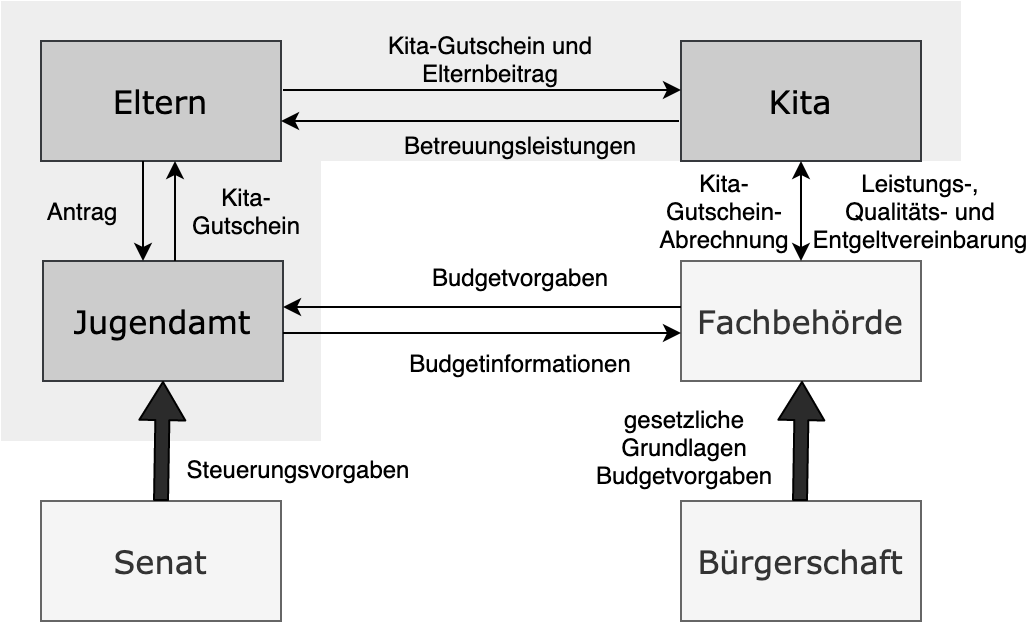
\includegraphics[keepaspectratio]{images/figure55.png}} \hfill{}

\caption{Abb. 5.5: Hamburger Gutscheinmodell (Brinkmann, 2010, S. 181,
zit. n.~Kolhoff, 2017, S. 9)}

\end{figure}%

\subsection{Objektfinanzierung}\label{objektfinanzierung}

Bei der Objektfinanzierung bzw. der direkten Finanzierung werden
öffentliche Mittel als Geldleistungen in Form von Zuwendungen von der
Europäischen Union, von Bund und den Ländern zur Erfüllung öffentlicher
Aufträge oder durch Kommunen im Rahmen ihres Budgets gewährt (Kolhoff \&
Bettig, 2013, S. 24). Die rechtliche Grundlage bilden hierzu
Leistungsverträge oder Bescheide, und es müssen in der Regel
haushaltsrechtliche Rahmenrichtlinien, Vergabegrundlagen sowie
entsprechende Auflagen und Bedingungen beachtet werden. Zuwendungen sind
in der Regel umsatzsteuerbefreit und müssen beantragt werden.

Direkte Finanzierungen können in zwei Formen gewährt werden (Kolhoff \&
Bettig, 2013, S. 4):

\begin{itemize}
\item
  \emph{Projektfinanzierung}: Projekte für selbstgewählte und noch nicht
  begonnene Aufgaben innerhalb eines freien Trägers können -- unter
  Zugrundelegung eines Finanzierungs- und Kostenplans -- mit
  öffentlichen Mitteln gefördert werden, um die im Rahmen der
  Maßnahmenumsetzung entstehenden Kosten zu decken.
\item
  \emph{Institutionelle Förderung}: Dabei handelt es sich um eine
  längerfristige Förderung von öffentlichen Aufgaben auf Basis von
  Wirtschafts-, Haushalts- und Stellenplänen, die durch die öffentliche
  Hand nicht selbst erbracht werden können (z. B. Einrichtung von
  Beratungsstellen).
\end{itemize}

Bei der Inanspruchnahme von Zuwendungen aus öffentlichen Mitteln können
verschiedene Finanzierungsformen unterschieden werden:

\begin{itemize}
\item
  \emph{Vollfinanzierung}: Es werden alle direkten und indirekten
  Ausgaben abgedeckt.
\item
  \emph{Anteilsfinanzierung}: Es wird nur ein bestimmter Prozentsatz der
  Gesamtkosten finanziert.
\item
  \emph{Festbetragsfinanzierung}: Für die Finanzierung steht ein Betrag
  in bestimmter Höhe zur Verfügung.
\item
  \emph{Fehlbedarfsfinanzierung}: Es wird nur die Deckungslücke zwischen
  tatsächlichen Ausgaben und den eingesetzten eigenen/fremden Mitteln
  finanziert.
\end{itemize}

\subsection{Nicht-öffentliche Finanzierung durch
Fundraising}\label{nicht-ffentliche-finanzierung-durch-fundraising}

\subsubsection{Was versteht man unter Fundraising?}\label{fundraising}

Unter \emph{Fundraising} versteht man die Beschaffung von Finanzmitteln
für soziale Einrichtungen jenseits staatlicher Förderung (Drittmittel),
die in der Regel ohne Anspruch auf Gegenleistungen gegeben werden.

Zu nicht-öffentlichen Finanzierungsmöglichkeiten zählen Mittel aus z.
B.:

\begin{itemize}
\item
  Spenden,
\item
  Mitgliedsbeiträgen,
\item
  Crowdfundingmaßnahmen,
\item
  Lotterien,
\item
  Stiftungen, Kirchen und von
\item
  Industrie/Unternehmen/Kooperationspartnern.
\end{itemize}

Die Wege und Möglichkeiten für Fundraisingmaßnahmen sind vielseitig. Im
Rahmen der Online Fundraising Studie von Altruja GmbH (2019, S. 28)
wurden die -- wie in \hyperref[figure56]{Abb. 5.6} ersichtlich --
aktuell verwendeten Fundraisingkanäle erhoben. In der Studie kam man zu
dem Ergebnis, dass nach wie vor das Post-Mailing (64,8 \%) der am
häufigsten gewählte Fundraisingkanal für Großunternehmen ist, gefolgt
von Förderungen aus Stiftungsgeldern (41,4 \%) und Online Fundraising
(41,4 \%). Bei mittleren Organisationen stellen nach deren Aussage die
Mitgliedsbeiträge (41,9 \%) und für Kleinunternehmen die Post-Mailings
(49,1 \%) die wichtigste Möglichkeit zu Kundenansprache im Fundraising
dar.

\begin{figure}

\pandocbounded{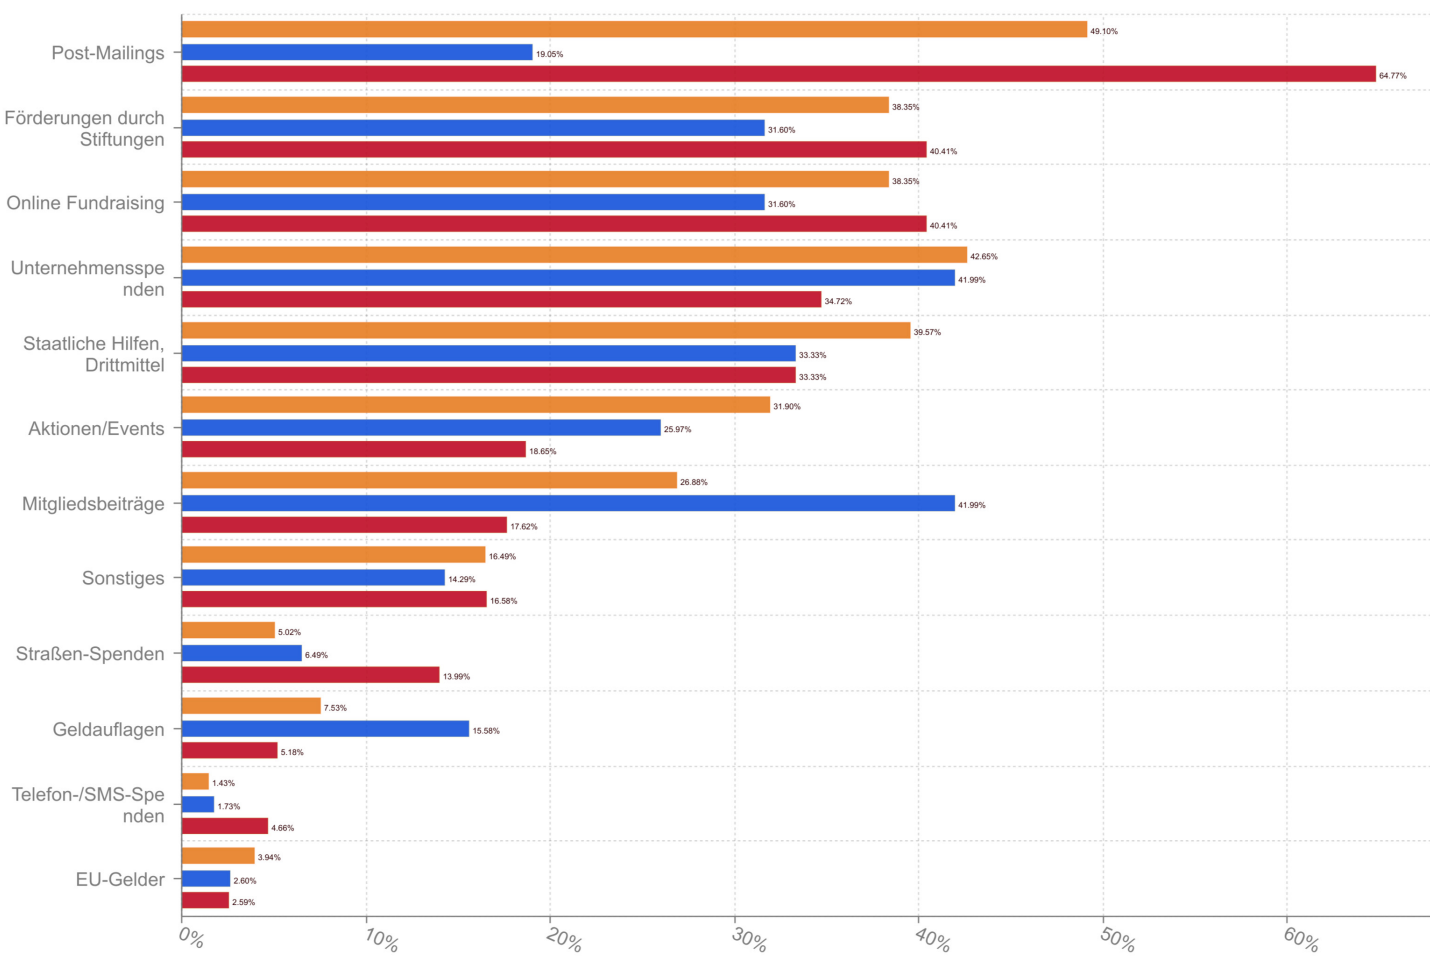
\includegraphics[keepaspectratio]{images/figure56.png}} \hfill{}

\caption{Abb. 5.6: Aktuell wichtigste Fundraisingquellen (Altruja GmbH,
2019, S. 28)}

\end{figure}%

Im Folgenden soll auf vier für die Existenzgründung im sozialen Bereich
wichtige Fundraisingaktivitäten eingegangen werden, die bei der
Finanzplanung Berücksichtigung finden sollten: Spenden, Sponsoring,
Stiftungsförderungen und Crowdfunding.

\subsubsection{Spenden}\label{spenden}

Bei Spenden handelt es sich um freiwillige Zuwendungen für
gemeinnützige, z. B. kulturelle, wissenschaftliche, politische oder
religiöse, Zwecke. Unternehmen können Geld- und Sachspenden oder auch
Zeitspenden (z. B. Entlohnung für ehrenamtliche Arbeit) erhalten, ohne
dafür eine konkrete Gegenleistung erbringen zu müssen. Rechtlich gesehen
handelt es sich dabei um eine Schenkung, die für die schenkende Person
steuerrechtlich als Sonderausgabe abzugsfähig ist.
Spendenempfänger*innen deklarieren eine Spende immer als Einnahme und
stellen entsprechend den Spender*innen eine Spendenbescheinigung aus.
Sozialunternehmer*innen sollten ein umfangreiches Spendernetzwerk
aufbauen und dies im Rahmen der Planung von Marketingaktivitäten
berücksichtigen.

\subsubsection{Sponsoring}\label{sponsoring}

Im Rahmen des Sponsorings werden Zuwendungen in Form von „Geld,
Sachmitteln, Dienstleistungen oder Know-how durch Unternehmen und
Institutionen zur Förderung von Personen und/oder Organisationen in den
Bereichen Sport, Kultur, Soziales, Umwelt und/oder den Medien'' (Bruhn
2019) zur Verfügung gestellt. Gegenüber einer Spende oder
Stiftungsförderung handelt es sich beim Sponsoring um ein in der Regel
umsatzsteuerpflichtiges Geschäft, bei dem eine Leistung gegenüber einer
Gegenleistung geschuldet wird. Die gesponserte Einrichtung erhält vom
Sponsor meist ein Entgelt. Als Gegenleistungen können beispielsweise
gemeinsame Veranstaltungen, Messeauftritte, Print-/PKW-Werbung, Logos
auf Kleidung, Publikationen oder Instandsetzungsarbeiten genutzt werden.
Davon erhofft sich das sponsernde Unternehmen eine Verbesserung des
eigenen Markenauftritts sowie des Firmenimages. Steuerlich gesehen kann
der Sponsor die zur Verfügung gestellten Mittel als Betriebsausgaben
angeben, die seinen Gewinn mindern (vgl. \hyperref[figure57]{Abb. 5.7}).

\begin{figure}

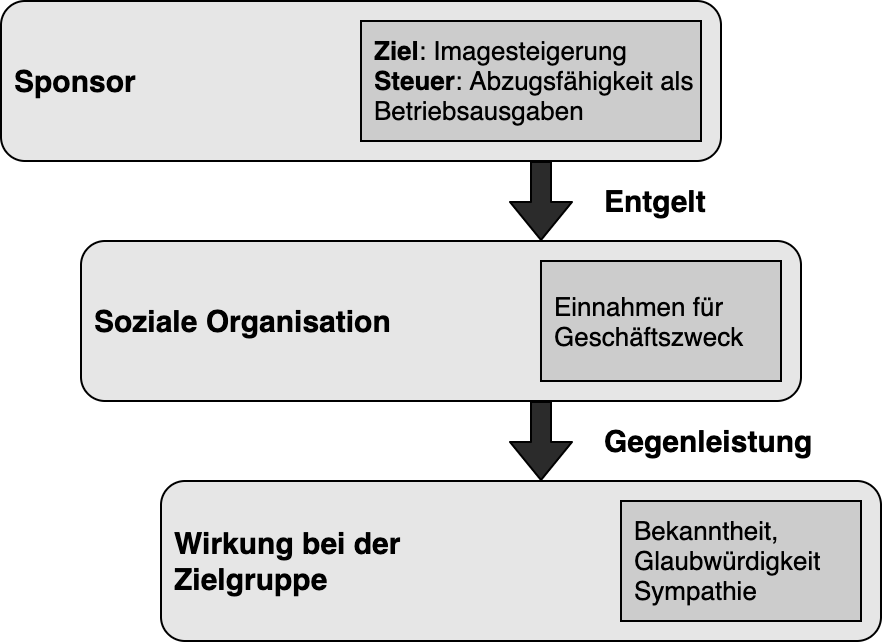
\includegraphics[width=0.6\linewidth,height=\textheight,keepaspectratio]{images/figure57.png} \hfill{}

\caption{Abb. 5.7: Sponsoring (eigene Darstellung)}

\end{figure}%

Sponsoring stellt nicht nur eine Einnahmequelle dar, sondern dient vor
allem auch der Erreichung von bestimmten Marketing- und
Unternehmenskommunikationszielen, wie in folgender
\hyperref[table53]{Tab. 5.3} dargestellt:

\begin{longtable}[]{@{}
  >{\raggedright\arraybackslash}p{(\linewidth - 2\tabcolsep) * \real{0.5000}}
  >{\raggedright\arraybackslash}p{(\linewidth - 2\tabcolsep) * \real{0.5000}}@{}}
\caption{Tab. 5.3: Ziele im Sponsoring und von sozialen Einrichtungen
(Kolhoff \& Bettig, 2013, S. 54)}\tabularnewline
\toprule\noalign{}
\begin{minipage}[b]{\linewidth}\raggedright
\textbf{Mögliche Ziele des sponsernden Unternehmens}
\end{minipage} & \begin{minipage}[b]{\linewidth}\raggedright
\textbf{Mögliche Ziele der gesponserten Einrichtung}
\end{minipage} \\
\midrule\noalign{}
\endfirsthead
\toprule\noalign{}
\begin{minipage}[b]{\linewidth}\raggedright
\textbf{Mögliche Ziele des sponsernden Unternehmens}
\end{minipage} & \begin{minipage}[b]{\linewidth}\raggedright
\textbf{Mögliche Ziele der gesponserten Einrichtung}
\end{minipage} \\
\midrule\noalign{}
\endhead
\bottomrule\noalign{}
\endlastfoot
- Imageverbesserung & - Suche nach neuen Finanzierungs- und/oder \\
- extern & Sachleistungsquellen \\
- intern (Stärkung der „Corporate Identity'') & \\
- Suche nach werbegeeigneten Personen und & - Suche nach Unterstützungen
organisatorischer \\
Gruppen und nach medienwirksamen Themen & Art (z. B. Hilfestellungen
beim Aufbau \\
und Veranstaltungen & eines Controllings) \\
- Vermarktung von Produkten im sozialen & - Nutzen von
Unternehmenskontakten zur \\
Bereich & Akquise von Geldern \\
\end{longtable}

Der Einsatz von Sponsoring sollte wohl überlegt werden, denn es gilt bei
dessen Nutzung einige Rahmenbedingungen, Chancen und Risiken abzuwägen,
die hier nur als Fragen dargestellt werden sollen (Kolhoff \& Bettig,
2013, S. 54-7):

\begin{itemize}
\item
  Ist die gesponserte Maßnahme für das gewünschte Ziel und für die
  Beteiligen passfähig?
\item
  Macht sich keine der beteiligten Institutionen (ob Sponsor oder
  Gesponserte) von Geldern und der Marketing- und Kommunikationspolitik
  der anderen Partei abhängig?
\item
  Ist nur die Sach- bzw. Dienstleistung Gegenstand des Sponsorings oder
  werden auch die Expertise und Beteiligung aller ermöglicht?
\item
  Sind die vertraglichen Grundlagen (Art, Umfang und Leistungen) genau
  geregelt?
\item
  Wurde die Maßnahme konkret geplant (Finanzbedarf,
  Öffentlichkeitsarbeit, Evaluation)?
\end{itemize}

\subsubsection{Stiftungen}\label{stiftungen}

Stiftungen fördern Personen, Maßnahmen, Projekte und Institutionen immer
nach Maßgabe bestimmter gemeinnütziger Zwecke und treffen bei
Förderanträgen eigene Ermessensentscheidungen. Voraussetzung für die
Inanspruchnahme von Fördermöglichkeiten bei Stiftungen sind daher
zuvorderst die Verwirklichung des jeweiligen Satzungszwecks durch die
beantragte Maßnahme. Gewährte Leistungen, die entweder vollständig oder
teilweise der Deckung aller beim sozialen Träger entstehenden Ausgaben
dienen, sind in der Regel steuerfrei. Die konkreten Fördermöglichkeiten
sind in einem breiten Spektrum angesiedelt, das von Projekten,
Stipendien und Förderpreisen bzw. Wettbewerben bis hin zur Förderung
diverser Austauschformate, Konferenzen, Reisen etc. reichen kann. Im
Rahmen der Existenzgründung sollte eingehend nach Stiftungen gesucht
werden, die bestimmte Maßnahmen des zu gründenden Unternehmens
unterstützen können. Hierfür ist die Stiftungsdatenbank wie z. B. die
vom \href{http://www.stiftungssuche.de}{Bundesverband Deutscher
Stiftungen} hilfreich.

\subsubsection{Crowdfunding}\label{crowdfunding}

Als weitere alternative Finanzierungsmöglichkeit bietet sich noch das
Crowdfunding an. Im Gegensatz zu anderen Formen des Crowdsourcings wie
z. B. Crowdwisdom, Crowdcreation, Crowdvoting steht beim Crowdfunding
die Akquise von (meist überschaubaren) finanziellen Mitteln von einer
relativ großen Gruppe von Personen über das Internet im Vordergrund, um
ein bestimmtes Projekt, ein Unternehmen oder Ziel zu finanzieren (vgl.
\hyperref[figure58]{Abb. 5.8}).

\begin{figure}

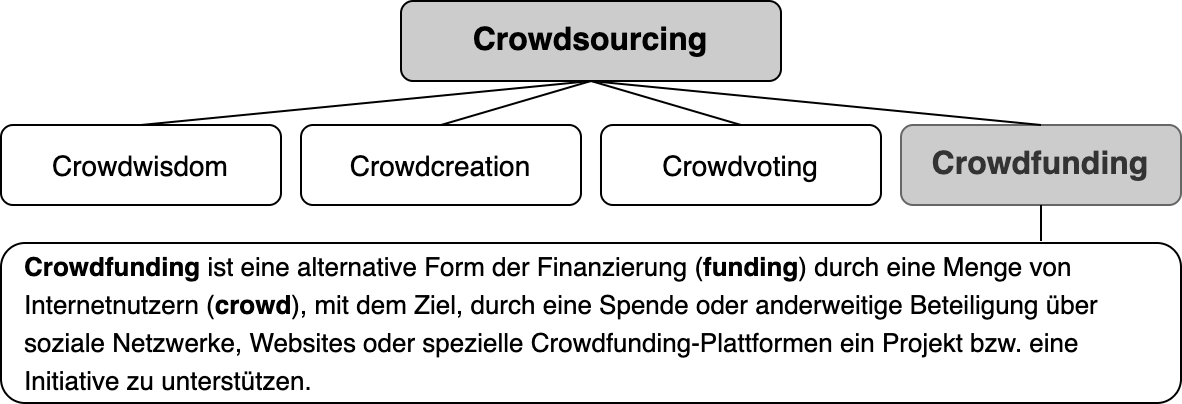
\includegraphics[width=0.9\linewidth,height=\textheight,keepaspectratio]{images/figure58.png} \hfill{}

\caption{Abb. 5.8: Definition von Crowdfunding (eigene Darstellung)}

\end{figure}%

Die Bedeutung von Crowdfunding hat in den letzten Jahren stark
zugenommen. Allein in Europa ist der Umfang an akquirierten Mitteln am
Finanzmarkt bzw. auf den Onlineplattformen von 1,13 Mrd. EUR auf 7,76
Mrd. EUR gestiegen (Ziegler et al., 2018, S. 22). In der
Crowdfunding-Praxis haben sich verschiedene Formen entwickelt, die es zu
unterscheiden gilt (\hyperref[figure59]{Abb. 5.9}):

\begin{itemize}
\item
  \emph{Donation-Based-Crowdfunding}: Für die Finanzierung eines
  Projekts, einer Kampagne oder einer Initiative werden Spenden
  akquiriert, wobei Spender keinen Anspruch auf Gegenleistung haben und
  nicht an dem finanzierten Projekt beteiligt werden sowie ihre Beiträge
  rein aus altruistischen und sozialen Motiven beisteuern.
\item
  \emph{Reward-Based-Crowdfunding}: Im Vordergrund steht eine Belohnung
  für die geleistete Spende, wobei Spender wie beim
  Donation-based-Crowdfunding keine Besitz- oder Stimmrechte erwerben,
  aber Anspruch auf materielle und/oder ideelle Rewards erhalten. Zu den
  Rewards können z. B. die Möglichkeit zum Vorverkauf von Produkten und
  Dienstleistungen, die Teilnahme an Veranstaltungen oder symbolische
  Auszeichnungen gehören.
\item
  \emph{Equity-Based-Crowdfunding} (auch \emph{Crowdinvesting}): Dabei
  werden auf einer Onlineplattform am Kapitalmarkt gehandelte
  Wertpapiere privater Unternehmen an Anleger vermittelt. Diese
  Transaktionen unterliegen nicht nur der Bankenaufsicht und bestimmten
  Finanzregulationen, da es sich i. e. S. um Finanzprodukte handelt, die
  einerseits Beteiligungs- und Besitzrechte beinhalten und bei denen
  andererseits die Funder Anspruch auf Erfolgs- bzw. Gewinnbeteiligungen
  erhalten.
\item
  \emph{Lending-Based-Crowdfunding}: Ähnlich dem
  Equity-based-Crowdfunding handelt es sich hierbei um ein
  kreditbasiertes Crowdfunding, welches Unternehmern die Möglichkeit
  einräumt, Mittel in Form von Krediten zu akquirieren, die über einen
  festgelegten Zeitraum und Zinssatz an die Kreditgeber zurückzuzahlen
  sind. Diese Finanzierungsform eignet sich insbesondere für
  Unternehmer, die nicht sofort auf Eigenkapital für ihr Start-up
  zugreifen können, sondern dies fremdfinanzieren müssen. Beim
  Peer-to-Peer-Lending (auch P2P-Lending) können Privatpersonen oder
  Unternehmen Geld über eine Onlineplattform, die Kreditgeber und
  -nehmer zusammenbringt, verleihen, was für Kreditnehmer häufig
  billiger als bei traditionellen Finanzinstituten ist und für
  Kreditgeber höhere Renditen verspricht.
\item
  \emph{Patronage-/Charity-based Crowdfunding}: Im Sinne des
  Mäzenatentums wird durch Einzelpersonen oder Unternehmen, die einen
  bestimmten Zweck unterstützen wollen, eine finanzielle Unterstützung
  gewährt, was meist auf längerfristige Projekte, Initiativen und
  Maßnahmen gerichtet ist und in Form von regelmäßigen (Teil-)Zahlungen
  ausgestaltet wird.
\end{itemize}

\begin{figure}

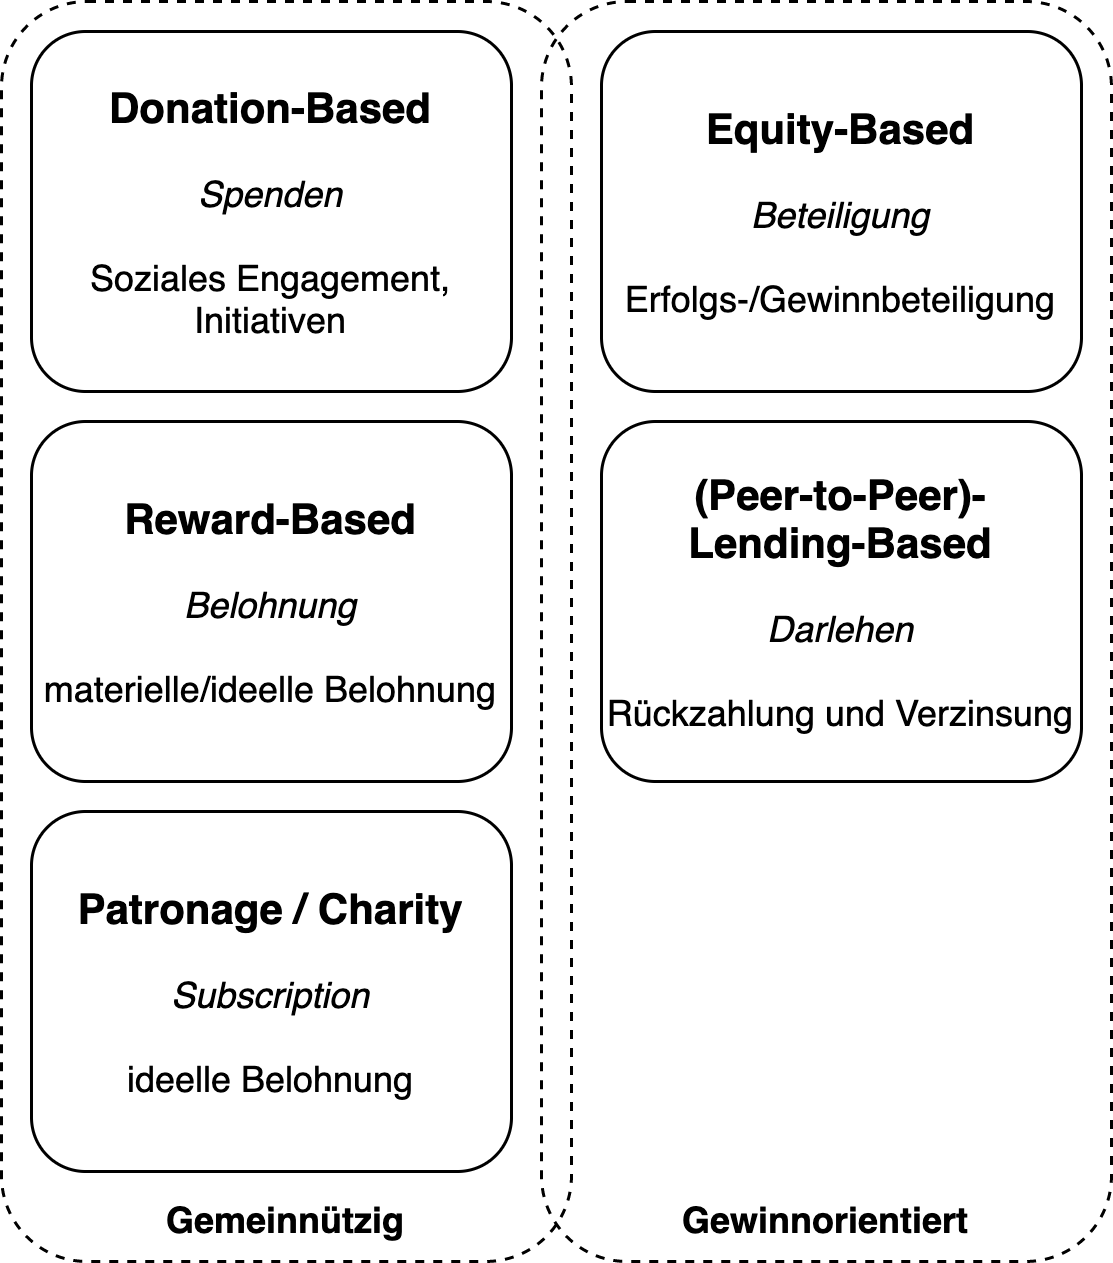
\includegraphics[width=0.5\linewidth,height=\textheight,keepaspectratio]{images/figure59.png} \hfill{}

\caption{Abb. 5.9: Crowdfunding-Formen (eigene Darstellung)}

\end{figure}%

In einer Studie von Mollick (2014) konnte festgestellt werden, dass sich
Unternehmer für das Crowdfunding von Produkten insbesondere dann
entscheiden, wenn sie neben dem Zuverdienst einen Berufswechsel
anstreben, Karriere machen wollen oder generell einen neuen Job suchen.
Ebenso konnte herausgefunden werden, dass es beim Crowdfunding nicht nur
darum geht, Drittmittel zu beschaffen und neue Projektpartner zu finden,
sondern damit auch ein agileres Vorgehen bei der Vergrößerung des
Kundenstamms und eine größtmögliche Steigerung der Bekanntheit des
Projektes (Öffentlichkeitsarbeit) erreicht werden kann. Besonders
erfolgreich sind Crowdfunding-Projekte immer dann, wenn es eine mehr
oder weniger emotional und kognitiv anspruchsvolle Story gibt, die
Mittelgeber und Initiatoren zusammenbringt, die Öffentlichkeitskampagne
möglichst so gestaltet wird, dass über den Einsatz von unterschiedlichen
Medien und sozialen Netzwerken eine breite Community aufgebaut wird und
dabei die virtuelle mit der realen Welt bestmöglich verbunden wird. Es
braucht seitens der Initiatoren häufig Ausdauer, Flexibilität und
Vertrauen in die zu finanzierende Unternehmung und es muss mit
denjenigen, die Mittel bereitstellen, ein regelmäßiger Dialog geführt
werden (z. B. über Newsfeeds, Statusmitteilungen, Blogs oder
Infobriefe).

\chapter{Was ist Management?}\label{management}

Das folgende Kapitel beschäftigt sich mit der Frage, was Management
eigentlich ist und (im Unternehmen) bezwecken soll. Es soll sowohl ein
geschichtlicher Rückblick unternommen werden als auch die Entwicklung
der theoretischen Grundlagen für das Management in der Sozialwirtschaft
nachgezeichnet werden.

Der Begriff Management hat ganz unterschiedliche Bedeutungen. Auf die
Frage, was denn Management sei, kann man -- um es mit den Worten von
\href{https://en.wikipedia.org/wiki/Charles_P._Kindleberger}{Charles P.
Kindleberger} (MIT) (1910-2003), der sich aber auf die
Volkswirtschaftslehre bezogen hatte, zu sagen -- so antworten: „It
depends.'' Diese Antwort ist eng verbunden mit den Grundaussagen der
sog. Contigency Theory
(\href{https://de.wikipedia.org/wiki/Kontingenztheorie_(F\%C3\%BChrungslehre)}{Kontingenztheorie})
in den Managementwissenschaften verbunden:

\begin{quote}
``argued that organizations evolve and change in quite different ways,
and must be managed in quite different ways, depending on a host of
factors both internal and extemal. Contingency theory was a slap in the
face to the notion ofthe \textquotesingle one best way\textquotesingle{}
. There is no \textquotesingle one best way\textquotesingle{} of
organizing and managing, says contingency theory, only the way that is
right for the place, time and people involved'' (Witzel, 2016, S. 190).
\end{quote}

Mit anderen Worten, wir stehen vor der Herausforderung, kontext-,
situationsabhängige Deutungen zu suchen. Der Wortstamm von ‚Management'
kann abgeleitet werden von ‚manus' (lat.: die Hand). Management bedeutet
also „etwas zusammenführen'' oder „an der Hand führen'' bzw. „mit der
Hand arbeiten''. Es geht im weiteren Sinne also um manuelle Tätigkeiten,
um etwas zu produzieren, herzustellen oder anzuleiten. Im engeren Sinne
heißt es soviel wie: mit den bloßen Händen arbeiten und lenken. In der
ursprünglichen Begriffsbedeutung zählt zu Management also das ‚tätige
Werk' und im erweiterten Sinne auch eine gewisse Kunstfertigkeit, wie
die Kompetenz und das Beherrschen aller notwendigen Schritte, die für
die Planung, Umsetzung und Steuerung von Arbeitsabläufen notwendig sind.

Im 19. Jahrhundert entstand dann die Grundidee, die auch heute noch für
die Betriebswirtschaftslehre letztendlich relevant ist, wenn wir uns mit
den Managementbegriffen auseinandersetzen: Management oder „to manage''
meint ganz allgemein die Fähigkeit, „in charge of (a business,
organization, or undertaking); run'' verantwortlich zu sein, z. B. für
eine Einrichtung oder eine gewisse Tätigkeit / einen Bereich und diesen
dann zu leiten. Dem
\href{https://www.oed.com/view/Entry/113210?isAdvanced=false&result=3&rskey=PtTs7q&}{Oxford
English Dictionary} (\emph{Manage}, n.d.) ist außerdem zu entnehmen:
``To succeed (despite difficulties) in accomplishing a task; to cope or
get by (esp.~financially); to contrive to get on \emph{with} something
which is barely adequate.'' Es geht dabei darum, auch etwas unter
schwierigen Umständen zu erreichen, zu schaffen oder zu erzielen. Eine
weitere Bedeutung von Management unterstreicht die Wichtigkeit dieser
Aufgabe. Management ist eine existenzrelevante Aufgabe („surviving'')
und dient allgemein dem Überleben. Management ist mit anderen Worten
also nicht auf die ökonomischen Zusammenhänge, in denen der Begriff
häufig verwendet wird, allein zu reduzieren.

Im britischen Kontext spricht man hauptsächlich dann von Management,
wenn „to direct / be in control of'' zählt. Hierbei geht es also um die
Tätigkeit des Leitens, Führens und Überprüfens von zu erreichenden
Zielen, was ursprünglich auf die administrative Rolle von Management
bezogen war. Der britisch-englischen Begriffsbedeutung zufolge meint
Management eher stärker die Tätigkeit, die wir in Leitungsaufgaben
ausüben, bzw. die Arbeitszusammenhänge, die in der Einrichtung vor dem
Hintergrund der Ebenen dargestellt werden. Im US-amerikanischen Kontext
wird eher der verwandte Begriff „executives'' verwendet. In Unternehmen
spricht man auch vom Executive Management, dem Vorstand. Ein Chief
Executive Officer (CEO) ist beispielsweise die*der Vorstandschef*in,
die*der oberste*r Repräsentant*in der Organisation nach innen und nach
außen. Management wurde seit jeher in diesem Sprachgebrauch als die
„science of administration'' (die wissenschaftliche Betrachtung der
Gestaltung und Verwaltung von Organisationen) angesehen (Hendry, 2013,
S. 1-2).

Wie werden wir den \emph{Allgemeinbegriff} Management verwenden? Wenn
wir von Management sprechen, geht es also um Umsetzung zielorientierter
und an ökonomischen Prinzipien orientierter Tätigkeiten bzw. Aufgaben,
die der Verwaltung, Steuerung und Gestaltung von Organisationen dienen.
Es können ganz verschiedenen Tätigkeiten dazu zählen bzw. in
unterschiedlichen Bereichen (vgl. Funktionsbereiche einer Einrichtung)
relevant werden. Neben dem Planungswesen gibt es Führungsprozesse, die
Personalentwicklung, das organisationsbezogene Management sowie
verschiedene Controllingaufgaben. Es gibt immer eine Vielzahl von
Managementaufgaben, die die Leitung im Blick haben und auch organisieren
muss.

Dann gibt es eine ganze Reihe von \emph{Managementtheorien,} die uns
dabei helfen, Grundlagen des Wirtschaftens zu verstehen und wie
bestimmte Abläufe in Organisationen funktionieren bzw. was vielleicht
„best practices'' sind, wie man die eine oder andere Aufgabe gut
umsetzen kann. Im Weiteren beschäftigen wir uns neben Managementtheorien
auch mit den verschiedenen Managementschulen, um zu verstehen, wie die
Beziehung zwischen Situation, Handeln und dem gewünschten Ergebnis
gestaltet ist. Noch einmal anders formuliert: Management bezeichnet
gewissermaßen die Tätigkeit, wie wir in Organisationen unsere Aufgaben
versehen. Die Theorie hilft uns dabei, diese Beziehung besser zu
verstehen, d.~h. in welcher Situation welcher Managementansatz sinnvoll
ist, wie Managementaufgaben gegliedert und organisiert werden können.
Mit Hilfe der Theorie können letztendlich auch die Ziele besser erreicht
und die Zielerreichung (\emph{performance}) gemessen werden.

Wir beschäftigen uns insbesondere mit Managementschulen und Aspekten,
die die \emph{„Human Side of Management''} thematisieren, also die
(human-/sozial-)wissenschaftliche Perspektive auf das Management
ausmachen. Schwerpunkt bildet dann also nicht die
Produktionsoptimierung, sondern wie die Zusammenarbeit mit Menschen in
Gruppen und organisiert und „gemanagt'' werden kann.

Wenn wir von Sozialmanagement sprechen, dann geht es um das Management
in und von sozialen Einrichtungen: „Die Theorie sozialen Managements
bezieht sich auf die zweckrationale Handhabung von sozialen Aufgaben,
die möglichst effektiv und effizient erledigt werden sollen'' (Wendt \&
Wöhrle, 2006, S. 26). Wir müssen uns mit der Theorie des
Sozialmanagements beschäftigen, um zu verstehen, wie die verschiedenen
sozialen Aufgaben, für die die soziale Einrichtung gegründet worden ist,
am besten umgesetzt werden können. Ein zweiter Aspekt ist dabei ebenso
von Bedeutung, nämlich dass Management stärker darauf schaut, wie man
Arbeitsaufgaben effektiver und effizienter erledigen kann. Wir
betrachten zwei Perspektiven, auf der einen Seite die soziale Aufgabe
und das professionelle Handeln und auf der anderen Seite die darauf
bezogenen wirtschaftlichen Fragestellungen. Dies stellt häufig ein
Dilemma dar, insbesondere wenn „Soziales'' und „Wirtschaften''
zusammengedacht werden müssen. Das Sozialmanagement versucht genau dafür
Ansätze zu entwickeln, um nicht die beiden Aspekte gegeneinander
auszuspielen. Soziale Aufgabenstellungen und wirtschaftliche Aspekte
sollen wie zwei Zahnräder komplementär ineinandergreifen: das Management
auf der einen Seite und die soziale Arbeit auf der anderen Seite.

Dann gilt es schließlich noch, den Begriff der
\emph{Betriebswirtschaftslehre} (BWL) zu klären. Wenn man sich mit den
betriebswirtschaftlichen Grundlagen beschäftigt, dann kann man
unterschiedliche Perspektiven einnehmen. Friedrich Vogelbusch
(Vogelbusch, 2017, S. 18) hat einmal versucht, BWL als wissenschaftliche
Disziplin vs.~Managementlehre zu unterscheiden (vgl. folgende
\hyperref[table61]{Tab. 6.1}). Die BWL als wissenschaftliche Disziplin
ist stärker zu verorten an Universitäten, wo neben der Lehre die
Erforschung von Grundlagen und Zusammenhängen im Vordergrund steht und
dann auch eine wissenschaftliche Untersuchung und ein
Erkenntnisgewinnungsziel dahinter steht, während die Managementlehre
stärker an den Fachhochschulen bzw. Handelshochschulen eine Rolle
spielt, weil es hier stärker um die Fertigkeiten und Fähigkeiten zur
Vorbereitungen auf die Berufspraxis geht.

Hier ist die Tabelle in Markdown-Format:

\begin{longtable}[]{@{}
  >{\raggedright\arraybackslash}p{(\linewidth - 4\tabcolsep) * \real{0.3333}}
  >{\raggedright\arraybackslash}p{(\linewidth - 4\tabcolsep) * \real{0.3333}}
  >{\raggedright\arraybackslash}p{(\linewidth - 4\tabcolsep) * \real{0.3333}}@{}}
\caption{Tab. 6.1: Aufgaben und Herangehensweise der
Betriebswirtschaftslehre (i. A. a. Martin Moog 2012, 18 zit. n.
Vogelbusch (2017, S. 18)}\tabularnewline
\toprule\noalign{}
\begin{minipage}[b]{\linewidth}\raggedright
\end{minipage} & \begin{minipage}[b]{\linewidth}\raggedright
\textbf{BWL als wissenschaftliche Disziplin}
\end{minipage} & \begin{minipage}[b]{\linewidth}\raggedright
\textbf{Managementlehre}
\end{minipage} \\
\midrule\noalign{}
\endfirsthead
\toprule\noalign{}
\begin{minipage}[b]{\linewidth}\raggedright
\end{minipage} & \begin{minipage}[b]{\linewidth}\raggedright
\textbf{BWL als wissenschaftliche Disziplin}
\end{minipage} & \begin{minipage}[b]{\linewidth}\raggedright
\textbf{Managementlehre}
\end{minipage} \\
\midrule\noalign{}
\endhead
\bottomrule\noalign{}
\endlastfoot
\textbf{Erkenntnisziel} & sucht nach: Gesetzmäßigkeiten {[}theoretisches
Erkenntnisziel{]} & Kenntnisse und Gesetzmäßigkeiten werden vermittelt,
um Manager zu befähigen, „gute'' Entscheidungen zu treffen \\
\textbf{Gegenstand} & Erkenntnisobjekt: Effizienz und Wirtschaftlichkeit
& es werden auch Sätze vermittelt, die wissenschaftlich nicht gesichert
sind. \\
\textbf{Praxisbezug} & die optimale Gestaltung ist eine normative Frage
& hierzu wird notwendiges Faktenwissen vermittelt (Regelwerke,
rechtliche und steuerliche Rahmenbedingungen) \\
\textbf{Lehrort} & Ort der Forschung und Lehre: Universitäten & Ort der
Lehre: Handelshochschulen, Fachhochschulen \\
\end{longtable}

Die \emph{BWL als wissenschaftliche Disziplin} verfolgt stärker ein
theoretisches Erkenntnisziel: Gibt es so etwas wie theoretische
Grundlagen? Der (theoretische) Erkenntnisgegenstand dabei ist die
Untersuchung bzw. Optimierung der Wirtschaftlichkeit und Effizienz.
Außerdem stehen tendenziell stärker normative Fragestellungen im
Vordergrund, also wie Organisationen gestaltet werden sollten. D. h. wir
versuchen mit Hilfe von wissenschaftlichen Aussagen zu beschreiben, wie
die Praxis funktioniert.

Im Gegensatz dazu hat die \emph{Managementlehre} eine andere
Zielrichtung. Ihr geht es darum, Erkenntnisse und Gesetzmäßigkeiten zu
vermitteln und gewissermaßen das Handwerkszeug in die Hände der
zukünftigen Managementpraktiker zu geben, damit bessere Entscheidungen
getroffen werden können. Man braucht Grundlagen des Managements, um
besser Entscheidungen zu treffen, und es wird dabei ggf. auch auf
praktische Handlungsempfehlungen zurückgegriffen und es werden Sätze
vermittelt, die (bisher noch nicht) wissenschaftlich abgesichert sind.
Ergänzend muss aber erwähnt werden, dass die Managementlehre zwar im
Regelfall praktisch orientiert ist und selbstverständlich auch
wissenschaftlich fundiert sein sollte.

In der \emph{Betriebswirtschaftslehre} haben wir es also,
zusammengefasst gesagt, mit verschiedenen Grundlagen und Konzepte zu
tun, die sich sowohl in der Praxis als auch in der Theorie entwickelt
haben bzw. ihren Ursprung haben. Diese müssen schließlich immer auf den
Prüfstand gestellt werden, um darüber zu diskutieren, was für die Praxis
geeignet und tauglich ist und was nicht. Aufgabe der Managementlehre ist
es, reflektiertes Wissen zu erwerben, eine Reihe von
Orientierungsmodellen kennenzulernen und diese aber von Situation zu
Situation, je nach Kontext und Handlungsabsichten sowie je nach der
gewünschten Zielstellung auszuwählen und anzuwenden. Dafür ist ein
gewisses Faktenwissen und die Kenntnis über entsprechende
Rahmenbedingungen unabdinglich, um dann ein „gute'' Managementpraxis
umzusetzen.

\section{Relevanz von
Managementtheorien}\label{relevanz-managementtheorien}

Im Folgenden wenden wir uns der Entwicklung der Managementtheorie bzw.
-geschichte seit dem 19. Jahrhundert zu. Selbstverständlich sind die
Ursprünge viel früher zu finden. So kann man beispielsweise bei
\href{https://en.wikipedia.org/wiki/Xenophon}{Xenophon}, einem
Zeitgenossen von Sokrates, in seinem Traktat
\href{https://www.gutenberg.org/files/1173/1173-h/1173-h.htm}{\emph{Oeconomicus}}
eine Abhandlung darüber finden, wie effektiv der eigene Hausstand bzw.
der eigene Hof verwaltet werden können. Der chinesische General,
Philosoph und Autor \href{https://en.wikipedia.org/wiki/Sun_Tzu}{Sun
Tzu} (auch Sunzi) hat das Buch
\href{https://de.wikipedia.org/wiki/Die_Kunst_des_Krieges_(Sunzi)}{\emph{Die
Kunst des Krieges}} hinterlassen, welches sich mit der Entwicklung und
Formulierung von Strategien beschäftigt und verschiedentlich im
strategischen Management Anklang gefunden hat.
\href{https://en.wikipedia.org/wiki/Niccol\%C3\%B2_Machiavelli}{Niccolò
Machiavelli}, der als Diplomat, Philosoph und Autor zur Zeit der
Renaissance gelebt und gewirkt hat, hat in seinen \emph{Discourses
}verschiedene Ansätze beschrieben, wie Macht innerhalb von
Organisationen verteilt und Konflikte bearbeitet werden können. Bei
\href{https://en.wikipedia.org/wiki/Luca_Pacioli}{Luca Pacioli}, dem
italienischen Mathematiker, finden wir in seinen
\href{https://en.wikipedia.org/wiki/Summa_de_arithmetica}{\emph{Summa de
arithmetica, geometria, proportioni et proportionalita}} einen frühen
Entwurf der Lehre von der doppelten Buchführung, einem Grundprinzip des
externen Rechnungswesens, welches heute noch Anwendung findet. Henry
Ford ist zwar kein Managementtheoretiker, er hat aber viele
Untersuchungen zu Beginn des 20. Jahrhunderts gefördert und sich bemüht,
die Administration der Ford-Werke entsprechend auf eine
wissenschaftliche Basis zu stellen.

Warum sollte man sich nun mit Managementtheorien auseinandersetzen?
Dafür gibt es verschiedene Argumente:

\begin{enumerate}
\def\labelenumi{\arabic{enumi}.}
\item
  Es gibt nicht „den richtigen Ansatz'' zum Management. Alles kann aus
  unterschiedlichen Perspektiven betrachtet und ggf. falsifiziert werden
  und das gilt auch für soziale Einrichtungen. Wir sollten also eine
  kritische und reflektiere Haltung einnehmen, wenn wir uns mit den
  verschiedenen Managementansätzen beschäftigen.
\item
  Theorien sind notwendig, da sie relevante Kriterien für das Verstehen
  von gemachten Erfahrungen liefern, Komplexität zu reduzieren verhelfen
  und ein kontinuierliches Lernen über die Welt ermöglichen. Mit anderen
  Worten, Theorien sind notwendig für die Praxis. Auch kann ein
  entwickeltes Modell helfen, komplexe Zusammenhänge darzustellen. Für
  jede gute Praxis braucht es auch eine gute Theorie und ohne Theorie
  kann die Praxis meist nur schwer gestaltet werden. Ein
  Theorie-Praxis-Transfer geht stets in zwei Richtungen und deswegen ist
  es auch Teil des Studiums des Sozialmanagements, dass man sich mit den
  theoretischen Grundlagen auseinandersetzen muss, um zu verstehen, wie
  bisher gemachte Erfahrungen reflektiert und Ansätze weiterentwickelt
  werden können.
\item
  Ziel der Auseinandersetzung mit der Managementtheorie ist es, Ansätze,
  Modelle und Konzepte kennenzulernen, diese kritisch zu beurteilen und
  das Essenzielle zu übernehmen, um damit eigene Perspektiven zu
  entwickeln.
\item
  Schließlich steht die Aneignung von reflexivem Wissen im Vordergrund.
  Metaphorisch gesprochen ist damit gemeint, dass wir in die Lage
  versetzt werden, in bestimmten Situationen, für bestimmte Aufgaben und
  bei unterschiedlichen Zielsetzungen einen Werkzeugkoffer nutzen
  können, aus dem ein passendes Werkzeug ausgewählt können, um
  Einrichtungen erfolgreicher zu leiten und gestalten.
\end{enumerate}

\section{Managementschulen}\label{managementschulen}

\subsection{Überblick}\label{ueberblick-managementschulen}

Bevor wir im Folgenden in die Vorstellung der einzelnen
Managementschulen einsteigen, erfolgt zunächst ein kurzer Überblick zur
Einordnung der verschiedenen Schulen (vgl. folgende
\hyperref[figure61]{Abb. 6.1}).

\begin{figure}

\pandocbounded{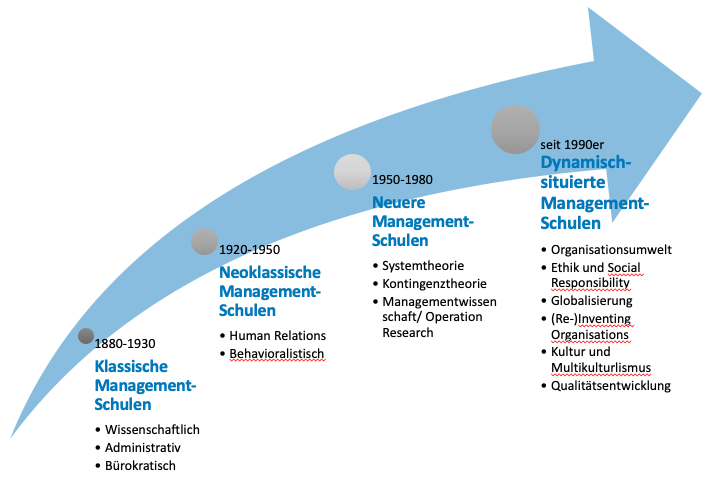
\includegraphics[keepaspectratio]{images/figure61.png}} \hfill{}

\caption{Abb. 6.1: Managementschulen im Überblick (eigene Darstellung)}

\end{figure}%

Die Ausführungen werden mit dem Ende des 19. Jahrhunderts bzw. Anfang
des 20. Jahrhunderts beginnen. Die sog. \emph{Klassischen Schulen (ca.
1880-1930)} haben sich mit einer wissenschaftlichen, administrativen und
bürokratischen Perspektive in Organisationen auseinandergesetzt. Im
Rahmen der \emph{Neoklassischen Managementschulen (ca. 1920-1950)} haben
verschiedene verhaltenswissenschaftliche Grundlagen Einzug gehalten. Von
Neoklassik spricht man deswegen, weil sie sich an den klassischen
Schulen abarbeiten, diese kritisch betrachten und weiterentwickeln. Im
Vordergrund steht dabei die Frage, wie die „menschliche Seite'' im
Management von Organisationen stärker berücksichtigt werden kann, also
z. B. Fragen der Motivation, des Empowerments und der
Personalentwicklung. Anschließend gilt es, sich mit den \emph{Neueren
Managementschulen (ca. 1950-1980)} auseinanderzusetzen. Der Begriff
„neu'' ist hier schon etwas abgenutzt und relativ zu betrachten. Diese
Managementschulen haben aus anderen Wissenschaftsbereichen verschiedene
Theorien aufgenommen, wie z. B. die System- und Kontingenztheorie. In
systemtheoretischen Perspektiven gehen wir davon aus, dass die gesamte
Organisation als ein lebendes und sich veränderndes System betrachtet
wird. Im Gegensatz dazu setzt die Kontingenztheorie gewissermaßen
voraus, dass wir in verschiedenen Situationen auch unterschiedlich
reagieren müssen und dementsprechend auch unsere Managementmethoden und
-ansätze situationsflexibel angepasst werden müssen. Mit einem stärker
naturwissenschaftlichen Impetus hat sich die Managementwissenschaft bzw.
das Operation Research herausgebildet. In diesem Zusammenhang geht es u.
a. um die Optimierung von Produktionsprozessen. Abschließend sind noch
die \emph{Dynamisch-situierten Managementschulen} zu nennen, die sich
seit den 1990er Jahren formieren. Es handelt sich dabei um eine nur noch
schwierig überblickbare Vielzahl und Vielfalt von Schulen, die sich
beispielsweise mit organisatorischen Rahmenbedingungen der
Organisationsumwelt (Welchen Einfluss haben externe Ereignisse auf uns
als Organisation?), Ethik und Social Responsibility (Wie können
Unternehmen soziale Verantwortung übernehmen und eine entsprechende
Berichterstattung umsetzen?), Einflüssen der Globalisierung (Welchen
Einfluss haben globale-vernetzte Lieferketten?), Ansätzen in der
Organisationstheorie (Wie können neue Formen von Organisationen gedacht
werden?), Kultur und Multikulturalismus (Welche Wissensrepertoire
umfasst das Interkulturelle bzw. Internationale Management?) und der
Qualitätsentwicklung (Was beinhalten Systeme der Qualitätssicherung?).

\subsection{Klassische
Managementschulen}\label{klassische-managementschule}

Beginnen wir zunächst mit den klassischen Managementschulen. Diese haben
sich mit der Anwendung wissenschaftlicher Erkenntnisse auf die
Verbesserung der Managementpraxis sowie auf den Erwerb und insbesondere
die Vermittlung von praktischem Wissen, Prinzipien und Ansätzen
beschäftigt. Wir befinden uns historisch gesehen in der Hochzeit der
industriellen Revolution. Viele technische Innovationen haben es
ermöglicht, Produktionsprozesse effektiver zu gestalten. Menschen zogen
aufgrund der Arbeit vom Land in die Stadt. In Großunternehmen, wie z. B.
in der Automobilindustrie wurden insbesondere Fließbandarbeiter*innen
gebraucht. Rationalisierungsprozesse standen immer wieder auf der
Tagesordnung. Das zugrundliegende Welt- und Menschenbild war immer noch
mechanistisch uns der arbeitende Mensch wurde als Produktionsfaktor
betrachtet. Arbeitsprozesse wurden so lange optimiert, bis das
beabsichtigte Ergebnis erreicht werden konnte. Das Prinzip von „Division
of Labor'' (u. a. Adam Smith) wurde genutzt, um Fließbandarbeiten in
viele kleinteilige manuelle und monotone Tätigkeiten zu zerlegen, sodass
jeder einzelne Prozess optimiert werden und zum Schluss hoffentlich eine
Produktions- und Ertragssteigerung erreicht werden konnte. In dieser
Zeit haben sich aufgrund der Prekarisierung von Arbeitsverhältnissen und
der ausbeuterischen Veranlagung so mancher Großindustrieller
verschiedentlich Arbeitnehmervertretungen herausgebildet.

Es gibt drei klassische Managementschulen, die im Folgenden anhand
ausgewählter Persönlichkeiten und Managementansätze näher beschrieben
werden:

\begin{itemize}
\item
  die wissenschaftliche Schule
  (\hyperref[wissenschaftliche-managementschule]{6.2.2.1}),
\item
  die bürokratische Schule
  (\hyperref[buerokratische-managementschule]{6.2.2.2}),
\item
  die administrative Schule
  (\hyperref[administrative-managementschule]{6.2.2.3}).
\end{itemize}

\subsubsection{Wissenschaftliche
Managementschule}\label{wissenschaftliche-managementschule}

Wenn von der „Scientific School of Management'' gesprochen wird, fällt
stets der Name
\href{https://en.wikipedia.org/wiki/Frederick_Winslow_Taylor}{\emph{Frederick
Winslow Taylor}}. Er ist insbesondere bekannt geworden durch die sog.
\emph{Taylorschen Prinzipen} (u. a. wissenschaftliche Methoden ersetzen
die Daumenregel, Produktivitätssteigerung geht mit Personalqualifikation
einher, Arbeitsprozesse sind von Zusammenarbeit bestimmt,
Gleichverteilung der Arbeit zwischen Vorarbeiter*in und Arbeiter*in).

\emph{Taylor} ist bereits damit verschiedenen Fragen nachgegangen, die
auch für unsere heutigen Arbeitszusammenhänge eine Bedeutung haben: Was
kann als bester wissenschaftlich-fundierter Weg angesehen werden, um die
Arbeitsleistung zu steigern? Neben der Optimierung von
Entlohnungsprozessen hat er sich auch damit beschäftigt, wie
Personalauswahl bzw. -akquise von Arbeitskräften stattfinden und deren
Fachwissen weiterentwickelt werden kann, damit diese spezialisierten
Aufgaben gut nachgehen können. Wie können Manager und Mitarbeitende, die
ein gemeinsames Ziel verfolgen, dazu beitragen, die Produktivität zu
steigern? In diesem Zusammenhang stellt er die These auf, dass jede
Tätigkeit in ihre kleinsten Teile zerlegt werden muss und anschließend
geprüft wird, ob sich damit der Produktionsprozess optimieren lässt. In
diesem Zusammenhang entwickelte er die Idee des \emph{differential rate
system}. Demnach soll den Arbeitskräften, die in der Akkordarbeit
besonders viel produziert haben, ein höherer Lohn, und zwar in
Abhängigkeit der Leistungsmenge, gezahlt werden. Das Ganze hat natürlich
seine Grenzen, da die Produktivität nicht bis ins Unendliche gesteigert
werden kann.

Historischer Hintergrund sind die industrielle Revolution und
Massenproduktion in Großunternehmen am Ende des 19. Jahrhunderts (vgl.
dazu im Folgenden (Conti, 2013). Die (Akkord-)Löhne der meist
ungelernten Arbeitnehmenden sind niedrig. Das prägende Menschenbild ist,
ähnlich wie bei der bürokratischen Schule, durch eine mechanistische
Weltsicht geprägt, wobei der Mensch als Mittel zum Zweck und als
wesentlicher „Produktionsfaktor'' zur Generierung und Maximierung der
Unternehmenserträge betrachtet wird. Organisationsstrukturen ähneln
einem Räderwerk einer fein geölten Maschine (vgl. Metaphern nach Gareth
Morgan). Gelegentlich muss eine mechanische Komponente ausgetauscht
werden, damit die Maschine weiterlaufen kann. Grundsätzlich wird im
Sinne des Taylorismus davon ausgegangen, dass eine Organisation durch
eine funktional differenzierte Arbeitsteilung und Spezialisierung der
einzelnen Prozessabschnitte gekennzeichnet ist. Es gibt klare
Hierarchien, in dem Sinne, dass wenige Manager (Vorarbeiter) für eine
Mehrzahl an Arbeitnehmer*innen einer Abteilung verantwortlich sind.
Aufgabenstellung von Managern und Arbeitskräften sind strikt voneinander
getrennt. Die gesamte Arbeitsorganisation basiert auf wissenschaftlichen
Prinzipien und Grundsätzen. Nach dem sog. Babbage-Prinzip werden im
Rahmen der Personalakquise Mitarbeitende mit spezifischen Kenntnissen
und Kompetenzen gezielt für Spezial(teil)aufgaben innerhalb der
Organisation ausgewählt und eingestellt. Wenn beispielsweise ein
Mechaniker gebraucht wird, dann erfolgt eine gezielte Suche nach
geeignetem Personal, das die exakte Ausbildung dafür hat (z. B.
Industriemeister). Unter Abwägung der vorgenannten Charakteristika kann
man Vor- und Nachteile dieser Managementsichtweise eruieren. Beginnen
wir mit den Vorteilen: Die Produktivität lässt sich nach dieser
Auffassung wie bei einer Maschine steuern: werden die
Produktionsfaktoren erhöht bzw. optimiert, kommt man im Anschluss zu
einem besseren Endergebnis und auch die Mitarbeitenden werden für diese
Mehrleistung entsprechend entlohnt. Wird in der Akkordarbeit mehr
geleistet, dann erhält der Manager der Abteilung sowie die gesamte
Abteilung einen Bonus (extrinsische Motivation). Betrachtet man die
Entwicklung der durchschnittlichen Schicht- bzw. Tagesarbeitszeiten über
einen längeren Zeitraum, so lässt sich ein wesentlicher Effekt erkennen:
aus Zwölfstunden- sind Zehn- bzw. Achtstundenschichten geworden.
Parallel dazu hat sich das soziale Sicherungssystem entwickelt und es
haben sich Gewerkschaften herausgebildet. Vorteilhaft ist außerdem, dass
sowohl Mitarbeitende als auch Vorgesetzte entsprechend flexibel entlohnt
werden. Es gibt aber auch eine Reihe von Nachteilen: Wie bei der
bürokratischen Schule findet am Fließband und in der Massenproduktion
eine sog. „Entfremdung der Arbeit'' statt. Menschen am Fließband werden
lediglich als Produktionsfaktoren betrachtet, die man beliebig skalieren
und freisetzen kann. Mitarbeitende werden nur in einem begrenzten Teil
des Unternehmens und ggf. monotone Aufgaben eingesetzt und kaum an der
Sinnproduktion der Organisation selbst beteiligt. Darüber hinaus muss
zur Akkordarbeit einschränkend angemerkt werden, dass sich die
Motivation der Arbeitskräfte durch die Entlohnung von Mehrarbeit zwar
steigern lässt, dies aber nicht bis ins Unendliche gelingt. Je nach
Wirtschaftslage gibt es entsprechend Fluktuationen in der Belegschaft.
Mit einem „verlorenen'' Arbeitnehmenden ist auch ein Wissens- und
Produktivitätsverlust verbunden (zumal neue Arbeitskräfte eine
Einarbeitungszeit benötigen). Bei Krankheit oder sonstigen
Arbeitsverhinderungen erhalten die Mitarbeitenden in der Regel keine
Lohnfortzahlung, was heute beispielsweise nach aktueller Gesetzeslage
selbstverständlich ist. Die hier beschriebenen Prinzipien des
Taylorismus und der Gestaltung von Arbeitszusammenhängen im Sinne
wissenschaftlicher Grundsätze sind später in den Managementansätzen
Computer-Integrated-Manufacturing (Rechnergestützte Prozessoptimierung)
und Business-Reengineering (Organisationsentwicklung) wiederaufgegriffen
worden.

Das hat letztendlich Taylor und dann später auch noch \emph{Frank Bunker
}und* Lillian Evelyn Gilbreth* dazu gebracht, sich mit Folgefragen
auseinanderzusetzen (Mees, 2013), wie z. B.: Wie können wir denn die
verschiedenen Produktionsschritte und die beanspruchte Zeit
visualisieren, sodass dann entsprechende Produktivitätssteigerungen
überhaupt möglich werden? Insbesondere Lillian Gilbert war es, die nach
dem frühen Tod ihres Mannes Frank die sog. \emph{Time and Motion
Studies} zu Ende geführt hat.

Als Schülerin von Taylor hat sie eine damals innovative Methode, die
Videographie bzw. Auswertung von Bewegtbildern eingesetzt. Mit Hilfe der
Kamera sollte festgestellt werden, wie anhand der Bewegungen der
Arbeitskräfte sowie derer Gesichtsausdrücke im Arbeitsprozess
festgestellt werden kann, wo Produktionsprozesse optimiert werden
können, um sowohl die Produktivität als auch die Motivation zu steigern.

\emph{Henry Laurence Gantt}, der zusammen mit Taylor verschiedene
Untersuchungen durchgeführt hat, war an einer Weiterentwicklung des
Taylorschen Entlohnungssystem interessiert. Es reichte seiner Meinung
nach nicht aus, dass ein Bonus für die Erfüllung der Tagesleistung
gezahlt wird, sondern es sollte noch einen weiteren motivationalen
Faktor geben. So experimentierte er mit der Idee, dass auch die
Vorgesetzten, wenn ihr Team eine Tagesleistung geschafft hatte,
entsprechend einen Bonus erhalten sollten. Auf Gantt geht auch die
Erfindung des sog. Gantt-Charts zurück, welches im Projektmanagement
genutzt wird. Dabei handelt es sich um ein graphisches Balkendiagramm
des Produktionsplans, in dem alle wichtigen Projektdaten vermerkt sind
und Prozesse, Verantwortlichkeiten, Ressourcen, Meilensteine, Aufgaben
und Abhängigkeiten dargestellt sind.

\subsubsection{Bürokratische
Managementschule}\label{buerokratische-managementschule}

In der bürokratischen Managementschule wurde u. a. untersucht, wie eine
perfekte Organisation aussehen muss. Max Weber ist einer der
bekanntesten deutschsprachigen Soziologen Anfang des 20. Jahrhunderts,
der sich auch mit dem Managementfragen beschäftigt hat. In seiner
Theorie zum bürokratischen (Organisations-)Modell geht er von
Großunternehmen als Strukturgebilde aus, die große Verwaltungsapparate
sowie eine strikte Hierarchie bzw. Einlinienstruktur (vgl. Abschnitt
\hyperref[organigramme]{Organigramme} im Buchteil
\hyperref[was-ist-eine-organisation]{Organisationsbezogenes Management}
besitzen. Seiner Meinung nach sind rationalistisch durchdachte
Organisationen sehr gut geeignet, um arbeitsteilige Prozesse effektiver
zu bewältigen, sodass jeder Bereich und jede Abteilung spezialisierte
Aufgaben umsetzen. Das übergeordnete Prinzip der Rationalität besagt,
dass alle Unternehmensaktivitäten allein am Zweck der Einrichtung
ausgerichtet und bemessen werden. Jeder Bereich ist der jeweils
übergeordneten Einheit unterstellt und berichtspflichtig, wobei die
übergeordnete Einheit für die Leistungsbeurteilung der Erreichung der
Ziele der jeweils zugeordneten Einheiten verantwortlich ist.
Arbeitsbeziehungen sind klar organisiert, Strukturen, Regeln und
Aufgabenverteilung festgelegt. Eine individuelle Weiterentwicklung
innerhalb der Organisation ist ebenfalls möglich. Eine sog.
Laufbahnförderung ist möglich, wenn man in einem bestimmten Bereich
seine Meriten gesammelt und für die höhere Aufgabe (z. B. Führungs- und
Leitungsaufgaben) qualifiziert ist. Im Sinne der funktionalen
Differenzierung besitzen bürokratische Organisationen eine Vielzahl von
spezialisierten und gut ausgebildeten Fachkräften in jedem Bereich. D.
h. es gibt für jede einzelne Aufgabe einen Bereich bzw. ein Sachgebiet,
das für eine ganz bestimmte formalisierte Teilaufgabe zuständig ist.
Antrags- und Genehmigungsprozesse sind ebenfalls geregelt. Das fängt bei
der den Antrag entgegennehmenden Stelle an, dann geht es über die
Sachbearbeitung und ggf. über den Amtsleiter. Letzterer gibt es wieder
zurück an den Sachbereich und dann wird der Antrag entweder genehmigt
oder nicht genehmigt.

Sicherlich hat diese Sichtweise der Organisation sowohl Vor- als auch
Nachteile: Diese Organisationsform stellte zur Zeit Max Webers eine
Innovation dar, weil insbesondere Großorganisation, wie beispielsweise
die Ford-Werke, sich darauf verlassen mussten, dass mit einer solchen
hierarchischen Struktur die Organisation entsprechend geführt und
geleitet werden kann. Auch verhindert eine funktionierende bürokratische
Organisationsform möglichst korruptes Verhalten, willkürliche
Entscheidungen und die Ausnutzung von Machtpositionen. Das Prinzip der
Sachlichkeit spielt eine besondere Rolle. Heute sind bürokratische
Organisationen noch in öffentlichen Einrichtungen, Ministerien und
Ämtern (z. B. Jugendamt) zu finden. Kritisch ist erstens anzumerken,
dass Organisationen nach diesem Modell einem mechanistischen Weltbild
folgen: Menschen werden als Produktionsfaktoren betrachtet, als Teil des
Systems, wo jeder seinen Beitrag leistet. Wenn aber die Menschen in
Organisationen nur programmatisch ihre Arbeitsaufgaben abarbeiten,
besteht die Gefahr, dass sich die Arbeit ggf. monopolisiert.
Problematisch ist zweitens, dass bürokratische Organisation eher
unpersönlich und als geschlossene Systeme wirken und der Mensch den
Strukturen und Prozessen in einem großen Verwaltungsapparat ausgeliefert
ist. Diese Idee ist dann später beispielsweise bei den situativen
Managementkonzepten wiederaufgenommen worden. Darauf wird weiter unten
bei den neueren Managementschulen noch einzugehen sein.

\subsubsection{Administrative
Managementschule}\label{administrative-managementschule}

Im Rahmen der administrativen Schule lag der Fokus darauf, verschiedene
Managementprinzipien und Managementfunktionen zu definieren, die man in
der Aus-, Fort- und Weiterbildung auf die Managementpraxis einsetzen
kann. Hier ist Henry Fayol zu nennen, der sich mit der Frage
auseinandergesetzt hat: Gibt es so etwas wie Prinzipien und theoretische
Grundlagen, auf denen Managementverhalten aufbaut? Fayol hat
Managementaufgaben, die letztlich Bestandteil in jedem klassischen
Lehrbuch waren. Im Management müssen vor allem folgende Aufgaben
vorhanden sein: Planung, Organisation, Führung, Koordination und
Kontrolle.

Diese Managementschule hat sich ebenso am Anfang des 20. Jahrhunderts
entwickelt. Ein bedeutender Vertreter ist Henri Fayol, der mehr oder
weniger universale Managementprinzipien und systematische Ansätze
entwickelt hat, von denen viele in der heutigen Managementausbildung
noch Gültigkeit haben, auch wenn häufig andere oder neue
Begrifflichkeiten verwendet werden (vgl. dazu im Folgenden Peaucelle \&
Guthrie, 2013). Der historische Kontext ist der gleiche wie bei der
bürokratischen und wissenschaftlichen Schule: Der Mensch wird als
Produktionsfaktor und die Organisation als ein Mittel zum Zweck der
Planung und Umsetzung von komplexen Produktionsprozessen angesehen. Im
Vordergrund stand die Klärung von Begriffen, die Entwicklung von
Managementinstrumenten und -methoden und die Definition einer optimalen
Aufbau- und Ablauforganisation sowie optimalen Gestaltung der
Organisation als System (z. B. Hierarchieverhältnisse in Form von
Organigrammen). Als problematisch hat sich schnell herausgestellt, dass
die von Fayol u. a. entwickelten Prinzipien keine universelle Gültigkeit
besitzen können, sondern an den Bedingungen von (westlichen)
Großunternehmen anknüpfen (Stichwort: Ethnozentrismus). Organisationen
werden fernerhin als abgeschlossene Systeme angesehen und die
Wechselbeziehung zur Umwelt sowie umweltbedingte Veränderungen werden
nicht ausreichend einbezogen. Zielsetzung und Strategien werden als
bekannt und transparent vorausgesetzt. Die meisten Prinzipien sind
vergangenheitsorientiert. D. h. wenngleich angenommen wird, dass die
entwickelten Erfolgsprinzipien theoretisch einen gewissen
Allgemeingültigkeitscharakter besitzen, so kann in der Praxis nicht ohne
Weiteres angenommen werden, dass die in der Vergangenheit erzielten
Ergebnisse auch in Zukunft wieder erreicht werden können (Stichwort:
Problem der Extrapolierung von Daten aus der Vergangenheit). Die
administrative Managementschule ist zum Ende des 20. Jahrhunderts bei
Peter Decker in seinem Ansatz des funktionalen Managements
wiederaufgegriffen worden (vgl. \hyperref[figure1]{Haus der BWL} im
Buchteil \hyperref[funktionsbereiche]{Betriebswirtschaftliche
Funktionsbereiche im Sozialunternehmen}.

\paragraph{Managementfunktionen und Managementprinzipien bei Henri
Fayol}\label{henri-fayol}

Auf Henri Fayol, den bekanntesten Vertreter der administrativen Schule,
geht die Lehre der 14 Managementprinzipien zurück. Es handelt sich dabei
um allgemeine Grundsätze, die für das Management jeglicher Einrichtung
von Bedeutung sind (Peaucelle \& Guthrie, 2013, S. 64):

\begin{enumerate}
\def\labelenumi{\arabic{enumi}.}
\item
  Jede Einrichtung muss sich zunächst Gedanken machen über die
  Organisation der \emph{Arbeitsteilung}, also die Verteilung und
  Strukturierung der einzelnen Aufgaben. Eine funktionale Arbeitsteilung
  steigert die Produktivität einer Einrichtung.
\item
  Es muss außerdem \emph{Autoritäten} geben, womit gemeint ist, dass
  Verantwortlichkeiten festgelegt werden müssen. D. h. nicht zwingend,
  dass wir eine von oben nach unten gegliederte Organisation haben
  müssen. Bei der Festlegung der Aufbauorganisation kann es natürlich
  verschiedene Gestaltungsformen geben, aber Fayol betont, dass man
  mindestens Verantwortlichkeiten und Rollen definieren muss.
\item
  Mit den Autoritäten ist auch das Prinzip der \emph{Disziplin} eng
  verbunden. Innerhalb jeder Organisation muss es Regeln geben. Werden
  diese gebrochen werden, müssen Sanktionen festgelegt werden. Wenn
  Aufgaben besonders gut erfüllt werden, sollte eine entsprechende
  Belohnung gegeben werden.
\item
  Daneben ist auch noch die \emph{Einheit der Auftragserteilung} von
  Bedeutung, womit gemeint ist, dass wenn Aufgabenstellungen besprochen
  und weitergegeben werden, metaphorisch gesprochen, nicht mehrere Köche
  den Brei verderben sollen. Ein spezifischer Auftrag sollte nur von
  einer vorgesetzten Person erteilt werden, nicht durch mehrere
  Leitungspersonen, da es sonst ggf. zu Verwirrung kommen kann und die
  ausführende Person in der Regel nicht allen Auftraggebern gerecht
  werden kann. Daher sollte für eine Einheitlichkeit in der
  Aufgabenweitergabe gesorgt werden.
\item
  Unmittelbar verbunden ist das Prinzip der \emph{Einheit der Leitung}.
  Demnach sollte es eine einheitliche Leitung geben. Es sollte vermieden
  werden, dass jeder Bereich „sein eigenes Süppchen kocht''. Es bedarf
  einer guten Abstimmung und Kommunikation zwischen den
  Einrichtungsteilen und Bereichen. Damit einher geht auch der Anspruch
  an die Leitungskräfte, die sich regelmäßig einen Überblick über ihren
  jeweiligen Bereich verschaffen müssen.
\item
  \emph{Unterordnung der Sonderinteressen unter das gemeinsame
  Gesamtziel}. Damit ist gemeint, dass die individuellen Interessen erst
  einmal zurückgestellt werden müssen. Es geht darum, bei jedweder
  Entscheidung zu prüfen, ob damit die organisationalen Ziele besser
  erreicht und dementsprechend auch umgesetzt werden können.
\item
  In Anlehnung an die Erkenntnisse, die durch die wissenschaftliche und
  durch die bürokratische Schule gesammelt worden sind, dass Arbeit
  entsprechend der Leistung entlohnt werden muss, gibt es bei Fayol auch
  das Prinzip der \emph{(flexiblen) Entlohnung}. Damit sind im weitesten
  Sinne leistungsbezogene Entgelte, wie z. B. Akkordlohn oder
  Bonus-/Prämienzahlungen oder Gewinnbeteiligungen gemeint.
\item
  Im Sinne des \emph{Prinzips der Zentralisierung} sollte jede
  Organisation gewissermaßen an ihren Binnenstrukturen arbeiten und
  diese stetig weiterentwickeln, sodass zentrale Aufgaben gebündelt
  werden und eine stetige Wissensaneignung und Qualifikation des
  Personals möglich ist (z. B. durch Intranet-Managementhandbuch). Das
  schließt nicht aus, dass auch bestimmte Entscheidungen dezentral
  getroffen werden können, aber es braucht in jeder Organisation das
  Gemeinsame und Verbindende (z. B. die Personalverwaltung und
  Buchhaltung eines sozialen Trägers mit verschiedenen
  Teileinrichtungen).
\item
  Das \emph{Rangordnungsprinzip} ist vom Prinzip der Autorität
  abgeleitet. In einer hierarchisch strukturierten Organisation ist die
  höchste Autorität oben beim „TOP-Management'' angesiedelt. Alle
  Arbeitnehmer*innen in den einzelnen Teilbereichen sind wie entlang
  einer Perlenschnur aufgefädelt. Es gibt einen klaren Dienstweg.
\item
  Das Prinzip der \emph{Ordnung} besagt, dass jede Person und jede Sache
  seinen Platz im Unternehmen hat. Mit anderen Worten, es gibt bestimmte
  materielle und personelle Ressourcen, die verwaltet werden müssen und
  die Leitung hat entsprechend die Verantwortung für die Bereitstellung
  der notwendigen Ressourcen, aber auch für die Akquise und
  Weiterentwicklung des Personals.
\item
  Beim Prinzip der \emph{Gleichheit} wird einerseits ein Wert und
  andererseits ein Grundsatz beschrieben. Gleichheit ist ein Aspekt der
  Organisationskultur und meint, dass Mitarbeitende einen gerechten
  Umgang im Unternehmen erwarten können und -- reziprok gesehen -- dem
  Arbeitgeber ihre Loyalität „schulden''.
\item
  Es braucht schließlich auch einen \emph{stabilen Führungskader}, da
  Führungskräfte für die Stabilität der Einrichtung verantwortlich sind.
  Ein ständiges Kommen und Gehen bzw. Personalwechsel fordert die
  Unternehmensführung ständig heraus.
\item
  \emph{Initiative} wird als wichtig anerkannt. Mitarbeitende sollen
  Initiative zeigen und sich mit kreativen Ideen einbringen können.
\item
  Fayol hebt schließlich die Förderung des \emph{Gemeinschaftsgeists}
  hervor: Das eigene Personal muss angeleitet und unterstützt werden.
  Wenn Konflikte entstehen, sollen diese entsprechend gelöst werden.
  Manchmal ist beispielsweise die mündliche und persönliche
  Kommunikation schneller als der schriftliche Weg,
\end{enumerate}

In seinem Hauptwerk~\emph{Administration industrielle et générale;
prévoyance, organisation, commandement, coordination, controle}
beschreibt Fayol darüber hinaus fünf grundlegende Managementfunktionen,
die sich immer noch in fast jedem Lehrbuch wiederfinden: (1) Am Anfang
eines jeden Prozesses steht die \emph{Planung} und Zielbildung. Auf
Basis der strategischen Unternehmensziele müssen die konkreten
Tätigkeiten und Aufgaben später konkretisiert und operationalisiert
werden. (2) Darüber hinaus gibt es die \emph{Organisation} (als
Tätigkeit): Strukturen, Prozess und Aufgaben müssen definiert und
arbeitsteilig ausgeführt werden. (3) Im Rahmen der \emph{Führung }geht
es um die Akquise, Anleitung, Weiterentwicklung des Personals. (4) Die
\emph{Koordinationsfunktion} dient dazu, dass Ressourcen und Mittel, die
zum Betrieb der Einrichtung notwendig sind, entsprechend zur Verfügung
gestellt werden. (5) Das \emph{Controlling} hat die Funktion, regelmäßig
zu überprüfen, ob die Effizienz und Effektivität sowie
Wirtschaftlichkeit aller Prozesse, Aufgaben und Entscheidungen in der
Einrichtung gewahrt ist. Es stellt sich die Frage, ob die gesetzten
Ziele erreicht wurden und ggf. neue Ziele gesetzt werden müssen.

\subsubsection{Kritik der Klassischen
Managementschulen}\label{kritik-klassische-managementschulen}

In den klassischen Managementschulen beobachten wir die Auswirkungen der
industriellen Revolution, Massenproduktion und Entmenschlichung von
Arbeitsverhältnissen. In dieser Zeit haben sich die Theoretiker aus
verschiedenen Perspektiven mit dem Management in Organisationen
beschäftigt. Die bürokratische Schule blickt auf die Systemstruktur, die
administrative Schule fokussiert Aufgaben, Prinzipien und Funktion des
Managements und die wissenschaftliche Schule sucht nach \emph{best
practices} auf Basis von wissenschaftlichen Untersuchungsmethoden. Im
Folgenden findet eine Würdigung und Kritik der einzelnen Denkschulen
statt.

Bei allen Errungenschaften und Neuerungen, die in den verschiedenen
klassischen Schulen erforscht worden sind, muss man durchaus noch einmal
eine kritische Sichtweise einnehmen. Zunächst ist das Menschen- bzw.
Weltbild zu reflektieren: Der Mensch wird als Produktionsfaktor und
Mittel zum Zweck, als ein Zahnrad im großen „Räderwerk'' der
Organisation angesehen. In der Neoklassik wird diese Sichtweise
aufgebrochen bzw. erweitert, indem Mitarbeitende nicht allein als
Erfüllungsgehilfen für die Erreichung bestimmter wirtschaftlicher
Zielsetzungen und der Produktivitätssteigerung angesehen werden. Es gibt
viele andere Einflussfaktoren auf die Arbeitsleistung und
Arbeitszufriedenheit, die in diesem Zusammenhang ebenfalls eine Rolle
spielen. Außerdem lässt sich die Produktivität nicht einfach bis ins
Ultimo steigern, sondern ist durch die Fähigkeit der jeweiligen
Arbeitskraft bestimmt und limitiert. Ebenso sind für die Gestaltung der
Arbeitsumgebung die Interessen der Mitarbeitenden sowie soziale
Bedürfnisse einzubeziehen, wie z. B. das Sicherheitsempfinden, die
Arbeitsplatzgestaltung und die Selbsteinschätzung in Form von
Entwicklungsgesprächen. Auf die letztgenannten Aspekte wird im Rahmen
der neoklassischen Schule näher einzugehen sein. Fraglich ist außerdem,
ob es den vielfach propagierten „besten Weg'' zum Management von
Einrichtungen überhaupt gibt oder dieser lediglich einen Mythos
darstellt. Managementinstrumente und -prinzipien sind nicht universell
gültig, sondern deren Einsatz hängt auch von den jeweiligen Situationen,
kontextuellen Faktoren, von der konkreten Person mit ihren Kompetenzen
und von den Gesamtzielen der Einrichtung ab. Ebenso muss hinterfragt
werden, ob die Behauptung, dass die Managementpraxis eine Art
wissenschaftliche Umsetzung ist, ggf. nicht haltbar ist.
Nichtsdestotrotz dienen wissenschaftliche Erkenntnisse und Methoden zur
Ermöglichung, Verbesserung und Weiterentwicklung der Managementpraxis.
Weitere Nachteile der klassischen Managementschule ergeben aus dem
Prinzip der funktionalen Arbeitsteilung, dass sich Arbeit weitgehend
monotoner gestaltet, eine Entfremdung der Arbeitsverhältnisse
stattfindet und generalistische Sichtweisen verloren gehen. Mit der
Zersplitterung von Prozessen in Teilaufgaben geht ein höherer
Kontrollaufwand einher.

Für die weiterführende Würdigung, Kritik und Reflexion der klassischen
Managementschulen können die folgenden Fragen herangezogen werden:

\begin{enumerate}
\def\labelenumi{\arabic{enumi}.}
\item
  Welche Besonderheiten zeichnet die klassischen Managementschulen aus?
\item
  Welche Aspekte sind wie relevant für das Management von sozialen
  Organisationen?
\end{enumerate}

\subsection{Neoklassische
Managementschulen}\label{neoklassische-managementschulen}

\subsubsection{Überblick}\label{uxfcberblick-1}

Wie die Bezeichnung zeigt, handelt es sich um eine Abgrenzung und
Weiterentwicklung von Ansätzen der klassischen Schulen. Fragen, die nun
im Vordergrund stehen, sind etwa: Wie können Manager und Mitarbeitende
besser zusammenarbeiten? Wie neben einer Steigerung der Produktivität
noch andere Aspekte wie z. B. die Qualität der Aufgabenübermittlung,
Motivation und Anreizsetzung in die Gestaltung von Arbeitsverhältnissen
einbezogen werden? Darüber hinaus versuchte man, sich kritisch von den
klassischen Schulen abzugrenzen, z. B. dass eine alleinige Fokussierung
auf die Standardisierung von Arbeitsprozessen in vielen Organisationen
nicht ausreichend ist sowie dass auch die Weiterentwicklung des Wissens
über Prozesse und verfügbare Technologien in Organisationen wesentlich
zur wirtschaftlichen Entwicklung einer Einrichtung beiträgt. Letzterer
Zusammenhang ist natürlich wesentlich komplexer als der in den
klassischen Schulen untersuchte Zusammenhang von „Produktionsfaktor
Arbeitnehmer'' zu „Outputsteigerung''. In der neoklassischen
Managementschule waren folgende Zusammenhänge von entscheidender
Bedeutung, wobei insbesondere die sozialwissenschaftlichen und
psychologischen Grundlagen in der Gestaltung von Arbeitsverhältnissen im
Vordergrund stehen:

\begin{enumerate}
\def\labelenumi{\arabic{enumi}.}
\item
  Wie können Mitarbeiter in ihren funktionalen Aufgaben motiviert bzw.
  unterstützt werden?
\item
  Welche Anreizsysteme wirken wie auf die (extrinsische/intrinsische)
  Motivationen von Mitarbeitenden?
\item
  Welche Effekte haben soziale Beziehungen, die Arbeitsplatzgestaltung,
  die Kommunikation innerhalb von Einrichtungen auf die Arbeitsleistung?
\end{enumerate}

Kurz zusammengefasst geht es in der neoklassischen Schule also um den
sozialwissenschaftlichen Blick auf das Management und um eine Kritik an
den klassischen Schulen.

\begin{enumerate}
\def\labelenumi{\arabic{enumi}.}
\setcounter{enumi}{1}
\tightlist
\item
  Bekannte Vertreter:innen und Untersuchungen der Neoklassischen
  Managementschule
\end{enumerate}

\subsubsection{Mary Parker Follet}\label{mary-parker-follet}

Beginnen möchte ich die kurze ideengeschichtliche Reise mit
\href{https://en.wikipedia.org/wiki/Mary_Parker_Follett}{Mary Parker
Follett (1868--1933)}. Sie hat sich als eine der ersten
Managementtheoretiker:innen insbesondere mit den sozialpsychologischen
Aspekten im Organisationsleben beschäftigt (vgl. im Folgenden Child,
2013). Auf Grundlage der Erkenntnisse der Psychologie entwickelte sie
eine holistische Sichtweise auf das Management. Nach ihrer Ansicht
sollte die Managementpraxis durch einen partizipativen Führungsstil
gekennzeichnet sein. Leadership ist danach nicht einfach als eine
Aufgabe bzw. Funktion zu verstehen, sondern es geht darum, Aufgaben
gemeinsam miteinander zu besprechen und Lösungen zu entwickeln.
Mitarbeitende sollten aus unterschiedlichen Gesichtspunkten für ihre
Tätigkeiten motiviert werden. Organisationen werden aus Parker Folletts
Perspektive als Netzwerke betrachtet. Alle Mitarbeitenden besitzen
unterschiedliche Kompetenzen und Fähigkeiten. Mitglieder einer
Organisation tragen jeweils mit ihren Fähigkeiten und Fertigkeiten dazu
bei, dass übergeordnete organisationale Ziele erreicht werden können.
Heterogenität wird in diesem Sinne als eine Stärke aufgefasst. Die
Netzwerke sozialer Beziehungen, die in Organisationen existieren, sind
also ebenso wichtig wie der in den klassischen Schulen untersuchte
Zusammenhang von Arbeitsleistung, Entlohnung und Erfolg.
Arbeitgeber*innen und Arbeitnehmer*innen übernehmen im weitesten Sinne
Funktionen wie Auftraggeber*innen und Auftragnehmer*innen. Das sollte in
der Gestaltung von Arbeitsverhältnissen ebenfalls eine gewisse Beachtung
finden, wobei darauf zu achten ist, dass bei der Lösungssuche und
Umsetzung ihrer Aufgaben Arbeitgeber*innen und Arbeitnehmer*innen
gleichzeitig zu beteiligen sind. Nach Parker Folletts Sicht kann
Management auch als eine Art „Kunstfertigkeit'' beschrieben werden: „the
art of getting things done through people'' (Zitat aus Biographie von P.
Graham,\,\emph{Mary Parker Follett: Prophet of Management}. Boston:
Harvard Business School Press, 1995). Mit anderen Worten heißt das, dass
Arbeit nur gelingen kann, wenn wir alle Aufgabenstellung aus Perspektive
der Mitglieder der Organisation selbst betrachten
(individuumsorientierte Managementsicht). Darüber hinaus wies sie darauf
hin, dass in die Entwicklung von Zielen und Strategien neben der
Innensicht von Organisationen auch das Arbeits- bzw. Organisationsumfeld
mit einbezogen werden soll.

\subsubsection{Hawthorne Studies}\label{hawthorne-studies}

Die \emph{Hawthorne Studies} wurden in den Jahren 1924 bis 1932 im Werk
Western Electric in den USA durchgeführt. Hawthorne ist ein Ort in der
Nähe von Chicago. Um sich einen Eindruck von den historischen
Hintergründen, Zielen und Ergebnissen der Untersuchung zu verschaffen,
ist dieses \href{https://youtu.be/W7RHjwmVGhs}{zeitgenössische Dokument}
sehr geeignet. Zunächst ist zu resümieren, dass Mitarbeitende mehr zu
leisten im Stand sind bzw. sich anders verhalten, wenn Sie bei der
Arbeit beobachtet werden. Beobachtung hat einen direkten Effekt auf die
Arbeitsleistung. Mit anderen Worten, sind Mitarbeitende in der Lage die
Performance zu steigern, wenn ihnen eine besondere soziale
Aufmerksamkeit zukommt. Das muss nicht grundsätzlich und kann nicht
allein durch finanzielle Entlohnung geschehen, wie das noch die
klassischen Managementschulen betrachtet haben, sondern es gibt noch
andere Einflussfaktoren. Der sog. „Hawthorne Effekt'', der in
verschiedenen Studien beschrieben wird, beinhaltet, dass die
Arbeitsleistung von Menschen bzw. Gruppen von Menschen durch
verschiedene Verhaltensfaktoren beeinflusst wird und nicht nur allein
durch die quantitativ gemessenen Outputs im Sinne der Akkordarbeit.
Dieser Effekt hat auch in den Sozialwissenschaften eine gewisse
Bedeutung erlangt, insbesondere der Gestaltung und Verwendung von
empirischen Datenerhebungsinstrumenten sollte man immer auch darauf
achten, dass der Untersuchungskontext und die Situation der Befragung
und Beobachtung einen Einfluss auf die Untersuchungsergebnisse hat (z.
B. sozial erwünschte Antworten). Weiterhin wurden in den erwähnten
Studien auch andere motivationale Einflussfaktoren auf
Arbeitsverhältnisse untersucht, wie Selbstwirksamkeitserfahrung,
Autonomiestreben und persönliche Beziehungen.

\subsubsection{Chester I. Barnard}\label{chester-i.-barnard}

Neben den Hawthorne Studies gibt es noch andere bekannte Vertreter*innen
der Neoklassik, die sich mit der Untersuchung von Arbeitsverhältnissen
beschäftigt haben. Dazu gehört beispielsweise \emph{Chester I. Barnard},
der für die Entwicklung der systemischen Sichtweisen im Rahmen des
organisationsbezogenen Managements steht. Organisationen sind demnach
als ein soziales System zu verstehen. In seinem Buch \emph{The Functions
of the Executives} beschreibt er die Organisation als ein durch
Zusammenarbeit geprägtes soziales System. Im Rahmen seiner
Akzeptanztheorie formuliert er, dass insbesondere formale
Organisationsziele besser erreicht und das Management stärker akzeptiert
werden, wenn Mitarbeiter sehen, dass ihre individuellen Bedürfnisse
befriedigt oder erfüllt werden. Das bedeutet, dass organisationale
Vorgaben und Anweisungen von Vorgesetzten stärker von Mitarbeitenden
akzeptiert werden und sie sich entsprechend für die Erfüllung ihrer
Aufgaben einsetzen, wenn sie erfahren, dass sich ihre Vorgesetzten um
ihre persönlichen Bedürfnisse sorgen. Darüber hinaus hat Barnard noch
ein anderes organisationales Phänomen beschrieben: die Zone der
Indifferenz. Damit ist der Bereich unseres täglichen Arbeitslebens
gemeint, wo Mitgliedern einer Organisation ein Freiraum in der
Gestaltung und Umsetzung von Arbeitsaufgaben gegeben wird und vom
Management keine direkten Vorgaben gemacht werden. Diese Zone der
Indifferenz soll einerseits eingerichtet und andererseits ermöglicht
werden. Darüber hinaus hat Barnard dann noch einen anderen Aspekt
hervorgehoben: die Bedeutung informeller Netzwerke. In Organisationen
kommt es immer auch auf das Expert*innenwissen einzelner Personen an. Es
muss nicht zwingend die Funktion eine Rolle spielen, sondern Personen
kennen sich in einem bestimmten Themenbereich sehr gut aus und auch
daraus kann sich eine Rolle im Unternehmen im Netzwerk ergeben. Darüber
hinaus betont Barnard, dass soziale Gruppen sind auch unabhängig von der
formalen Struktur, d.~h. in der Kaffee- oder Raucherecke bzw. beim
Flurfunk miteinander über arbeitsorganisatorische Dinge kommunizieren.
Es sind eben nicht zwingend nur die formalen Strukturen, die zum
Gelingen bzw. zur Entwicklung von Organisationen beitragen, sondern auch
die persönlichen Kontakte und direkten Interaktionen, die letztendlich
innerhalb von Einrichtungen von großer Bedeutung sind (vgl. dazu
Abschnitt \hyperref[organisationskultur]{Organisationskulturen}.

\subsubsection{Human Relations}\label{human-relations}

Abschließend soll noch ein Blick in die \emph{Human Relations Bewegung}
gerichtet werden. Elton Mayo (1933) und Fritz Roethlisberger et
al.~(1939) hatten nicht nur im Rahmen der Hawthorne Studies
mitgearbeitet, sondern entwickelten auch verschiedene Ideen, die für die
Neoklassische Managementschule von Bedeutung sind. Einerseits wurde ein
mechanistisches Weltbild abgelehnt und stattdessen vom Bild des Menschen
als einem sozialen Lebewesen ausgegangen. Mit Human Relation wird
gewissermaßen die menschliche Seite des Managements betont. Im Gegensatz
zur klassischen Schule stehen damit stärker die sozialen Bedürfnisse und
weniger die rationalistisch-ökonomischen Anreizsetzung im Vordergrund.
Mit sozialen Bedürfnissen sind beispielsweise die Arbeitsbedingungen,
die Qualität der Zusammenarbeit oder Mitarbeitermotivation gemeint, die
ebenfalls eine Wirkung auf die Arbeitsleistung haben. Darüber hinaus
wurde von den Autoren festgestellt, dass sich die personale Identität,
Loyalität und Identifikation mit der Organisation insbesondere durch die
interpersonalen Beziehungen (weiter-)entwickelt. Mithin hat die
Kommunikation der Mitarbeitenden untereinander und deren
Wissensaustausch eine Auswirkung auf die (Arbeits-)Motivation. Weiterhin
wurde beschrieben, dass Mitarbeitende in der Regel positiv auf Anreize
reagieren, insbesondere vom Management und von den Kolleg*innen sowie
den Kunden- bzw. Klient*innen. D. h., es muss von Seiten der Leitung
darauf Einfluss genommen werden, wie sich bestimmte Mitarbeitende in der
Einrichtung einbringen können. Darüber hinaus spielen aber auch
Gruppenprozesse eine große Rolle. Die soziale Kohäsion (=
Teamzusammenhalt) in Peer-Gruppen hat einen stärker motivationalen
Effekt als monetäre Anreize und Kontrollen (vgl. Beobachtungseffekt im
Rahmen der Hawthorne Studies). Individuell-persönliche Bedürfnisse
sollen zwar nicht im Mittelpunkt stehen, sollen aber aktiv eingebracht
werden können. Wenn ich aufmerksam beachtet werde, dann bringe ich mich
auch entsprechend in das Team besser ein und damit lässt sich dann auch
die Gruppenleistung steigern, also zwischen individueller Motivation und
der Auswirkung auf die Teamleistung gibt es einen ursächlichen, wenn
auch komplexen Zusammenhang.

\subsubsection{Kritik an der Neoklassischen
Managementschule}\label{kritik-an-der-neoklassischen-managementschule}

Abschließend ist auch die neoklassische Schule einer Kritik zu
unterziehen. Wir haben erstens gelernt, dass eben die sozial- und
verhaltenswissenschaftlichen Aspekte die Erkenntnisse der klassischen
Schulen ergänzen. Während bei letzteren noch Zusammenhänge zwischen den
ökonomischen Prinzipien, der Arbeitsleistung und dem Unternehmenserfolg
im Vordergrund standen, liegt der Fokus der Neoklassik verstärkt auf den
Menschen und den sozialen Belangen, Bedürfnissen und Motivationen
innerhalb der Organisation. Im Vordergrund stehen dabei Prinzipien wie
die Partizipation, Selbstverwirklichung und Empowerment (Mary Parker
Follett). Darüber hinaus ist der Fokus auf die systemische
Funktionsweise und die Komplexität der gesamten Einrichtung zu richten
(Chester I. Barnard). Ebenso wird hervorgehoben, dass die Existenz von
informellen Netzwerken innerhalb von Einrichtungen von Bedeutung ist.
Das wird uns dann im Weiteren beschäftigten müssen. Kritisch ist
gegenüber der Neoklassik einzuwenden, dass Anreizsetzungen immer auch
kontext-, situations- und personenabhängig sind. Dieser Aspekt spielt
letztlich in den neuen Managementschulen eine besondere Rolle.

\subsection{Neuere Managementschulen}\label{neuere-managementschulen}

\subsubsection{Überblick}\label{uxfcberblick-2}

Die neueren Managementschulen lassen sich in die 1950er bis 1980er Jahre
einordnen. Genauer gesagt, handelt es sich hierbei um verschiedene
Teilschulen, die sich aufbauend auf den Forschungsergebnissen und
Erkenntnissen der Klassik und Neoklassik in verschiedene Richtungen
weiterentwickelt haben. In diesem kurzen Überblick soll auszugsweise auf
die situationstheoretischen, systemtheoretischen und
managementwissenschaftlichen Ansätze eingegangen werden.

\emph{Situationale Ansätze} sind eng dem Kontingenzparadima verhaftet.
Kontingenz heißt, dass etwas entweder nicht verfügbar oder nicht sofort
greifbar ist. Kontingenzbewältigung heißt, dass wir versuchen die
Komplexität, Ungewissheit und Offenheit von Situationen zu überwinden
und in uns unbekannten Situationen einen Lösungsweg entwickeln möchten.
In Bezug auf die Managementlehre ist hiermit gemeint, dass es diesen
„besten Weg'', von dem die klassischen Schulen oft gesprochen haben,
eben nicht gibt. „The best way of Management'' ist sozusagen ein Mythos.
Alle Prinzipien, Ansätze und Methoden besitzen eine situationale
Abhängigkeit. Entscheidungen sind grundsätzlich abhängig von
verschiedenen Faktoren wie z. B. von der Kompetenz und dem
Ausbildungsgrad der Mitarbeitenden, dem Kontext (Fachliches
vs.~Leitungsthema), von der Branche etc. So lässt sich etwa der
Taylorismus nicht ohne Weiteres auf soziale Einrichtungen übertragen.
Ziel der situationalen Theoriebildung ist es daher, kontext-,
situations- und individuumsabhängige Ansätze zu entwickeln, die uns in
die Lage versetzen, in bestimmten Situationen, bestimmte Methoden,
Werkzeuge und Konzepte umzusetzen.

Die \emph{systemtheoretische Perspektive}, die sich schon parallel zur
Neoklassik (z. B. bei Chester I. Barnard) entwickelt hatte, hat eine
stärkere Präsenz entwickelt. Dabei wurde stets versucht, das Netzwerk-
und Systemdenken auf das Leben in und mit Organisationen zu übertragen.
Theoretische Grundlagen lieferten insbesondere die
Informationswissenschaften bzw. technisch orientierten Wissenschaften.
Die Kybernetik beschäftigt sich beispielsweise damit, wie eigentlich
Regelsysteme funktionieren. In der Betriebswirtschaftslehre gehört das
St.~Galler Management Modell u. a. zu den systemtheoretischen Ansätzen.
Das Modell versetzt uns in die Lage, die verschiedenen Teilsysteme
innerhalb und außerhalb von Organisationen (z. B. Finanzen, Personal,
Organisation, Marketing usw.) im Überblick zu behalten, um die
Einrichtung sinnvoll gestalten und leiten zu können. Und die
Systemtheorie besagt, dass die Kommunikation zwischen den Subsystemen
genau den Verbindungspunkt und die Kopplung darstellt, wie mit der
Komplexität der Aufgaben innerhalb des sozialen Systems Organisation
umgegangen werden kann.

In den stärker durch mathematisch-naturwissenschaftliche Erkenntnisse
geprägten \emph{Managementwissenschaften bzw. das Operation Research}
hat man sich u. a. die Frage gestellt, wie bestimmte
Entscheidungsprozesse mathematisch modelliert, Wahrscheinlichkeiten für
den Eintritt von bestimmten Ereignissen berechnet sowie
Entscheidungsgrößen identifiziert werden können. Ein Beispiel für diese
Managementschule ist der Entscheidungsbaum im Rahmen der
Investitionsrechnung oder im Kontext anderer utilitaristischer Ansätze.
Beispielsweise könnte man überlegen, ob man sich ein bestimmtes
Kleidungsstück kaufen möchte. Dabei würde man zunächst nach allen
relevanten Faktoren suchen, die Einfluss auf die Entscheidung haben
(Identifikation). Danach müssen die Eintrittswahrscheinlichkeiten bzw.
Gewichtung dieser Einflüsse quantifiziert werden (Quantifizierung).
Schließlich kann man dann den Erwartungswert für die Entscheidung
errechnen und ggf. mit alternativen Entscheidungen vergleichen, um die
(empirisch gesehen) optimale Entscheidung bzw. beste Kaufentscheidung
herauszufiltern (Filtration). Für unser Beispiel gesprochen können man
dann entsprechend abwägen, ob das T-Shirt oder die Bluse die bessere
Entscheidung darstellt und -- unter Abwägung unterschiedlicher Faktoren
-- nützlicher erscheint. Im Sozialmanagement haben diese
Managementwissenschaftlichen und Operation Research-Ansätze nur eine
untergeordnete Bedeutung.

\subsubsection{Theorie des Situationalen Führens nach Hersey und
Blanchard
(1982)}\label{theorie-des-situationalen-fuxfchrens-nach-hersey-und-blanchard-hersey1982leadership}

Wie oben beschrieben geht die Theorie des situationalen Führens auf die
Kontingenztheorie zurück. Der Ansatz ist schon historisch betagt, soll
hier aber als ein Beispiel fungieren. Es handelt sich um einen
zweidimensionalen Ansatz. Auf der X-Achse im Diagramm ist die
Aufgabenorientierung dargestellt. Damit ist der Grad an Aufmerksamkeit
und Detailgenauigkeit gemeint, inwieweit die Vorgesetzten klare Vorgaben
für die Umsetzung der besprochenen Aufgabe formulieren müssen. Hierbei
wird zwischen niedriger und hoher Aufgabenorientierung differenziert, um
damit den Reifegrad der Mitarbeitenden zu operationalisieren. Mit
anderen Worten: es wird versucht, das Kompetenzniveau der Mitarbeitenden
einzuschätzen. Hierbei muss man beachten, dass der Zusammenhang genau
umgekehrt ist: eine niedrige Aufgabenorientierung zeugt von einem hohen
Reifegrad, also einer hohen Kompetenz der Mitarbeitenden. Demnach muss
bei einer Aufgabenbesprechung nicht allzu sehr ins Detail gegangen
werden. Und umgekehrt ist bei einer hohen Aufgabenorientierung zu
erwarten, dass die betreffenden Mitarbeitenden über wenig Kompetenzen im
Aufgabenbereich verfügen. Auf der Y-Achse des Diagramms wird das
Beziehungsverhältnis zwischen Vorgesetzten und Mitarbeitenden
dargestellt. Auch hier gibt es eine Skala von niedrig bis hoch. Wenn die
Beziehungsorientierung hoch ist, wird vom Vorgesetzten ein stärker
persönlicher „Draht'' gesucht, stärker Unterstützung gegeben, häufiger
Lob ausgesprochen und Mitarbeitende motiviert. Bei niedriger
Beziehungsorientierung ist die Qualität des
Vorgesetzten-Mitarbeitenden-Verhältnisses etwas oberflächlicher (vgl.
\hyperref[figure62]{Abb. 6.2} nach (Pelz, 2004)).\footnote{Diese
  Abbildung stammt aus dem Buch von Pelz (2004).}

\begin{figure}

\pandocbounded{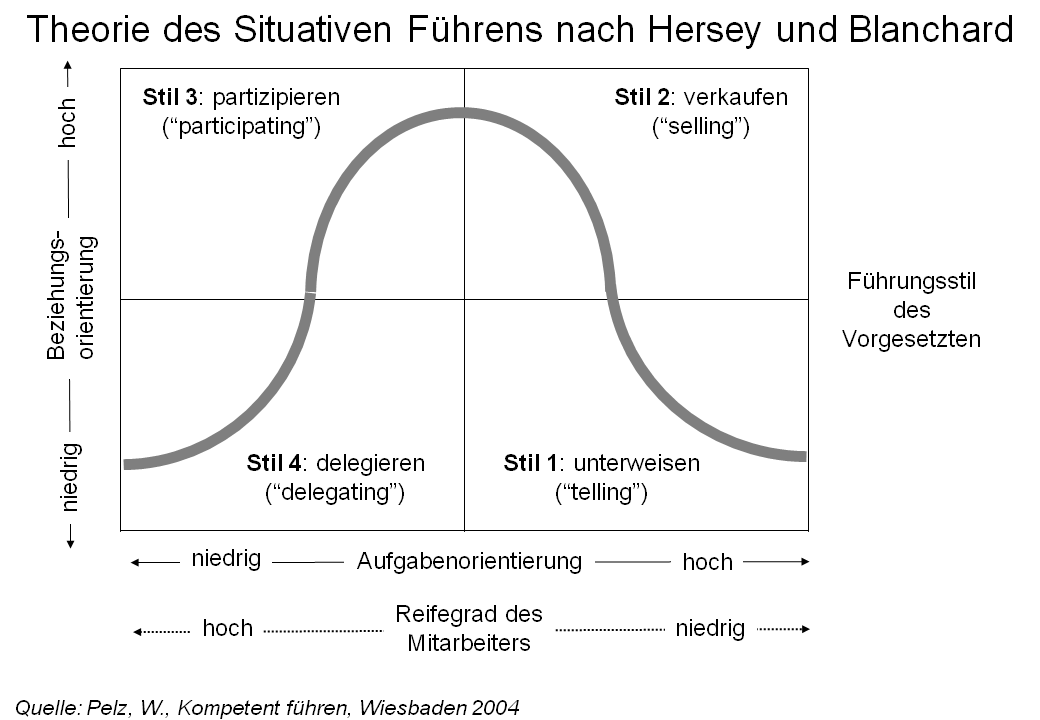
\includegraphics[keepaspectratio]{images/figure62.png}} \hfill{}

\caption{Abb. 6.2: Situatives Führen nach Hersey und Blanchard (1982)
(Pelz, 2004, Lizenz: CC BY SA 3.0,
\href{https://de.wikipedia.org/wiki/Datei:Theorie_des_Situativen_Fuehrens_nach_Hersey_und_Blanchard.png}{Link})}

\end{figure}%

Durch die Unterteilung in hohe und niedrige Grade der Beziehungs- und
Aufgabenorientierung ergeben sich vier Quadranten im Koordinatensystem.
Beginnend von rechts unten können im Zeitverlauf gegen den Uhrzeigersinn
unterschiedliche situativ-bedingte Führungsstile beschrieben werden.
\emph{Erstens}, wenn der Reifegrad der Geführten nicht so hoch ist, also
die Person noch nicht so viele Kompetenzen in betreffenden Bereich
gesammelt hat und die Beziehungsorientierung niedrig ist, z. B. weil
bisherig noch keine ausreichenden gemeinsamen Arbeitserfahrungen
existieren, dann sollte die Aufgabenstellung explizit und ausführlich
besprochen werden („Telling'' bzw. „Unterweisung''). Im Quadranten oben
rechts wird \emph{zweitens} hervorgehoben, dass in dieser Situation
Mitarbeitende über einen noch nicht so umfangreichen Kenntnisstand im
betreffenden Arbeitsbereich verfügen und eine hohe
Beziehungsorientierung seitens der Vorgesetzten, sprich gemeinsames
Erfahrungswissen, existieren. In dieser Situation steht schließlich das
„Verkaufen'' bzw. „Selling'' im Vordergrund. Mit anderen Worten, es
sollen die Mitarbeitenden von der Wichtigkeit der Aufgabenstellung
überzeugt werden und es muss erläutert werden, warum es so wichtig ist,
dass diese Aufgabe für die Einrichtung von hoher Bedeutung ist.
\emph{Drittens} wird im Quadranten links oben, ein
beteiligungsorientierter Führungsstil hervorgehoben („Participating''
bzw. „Partizipation''). In diesem Fall ist die Aufgabenorientierung
niedrig, das heißt also, die betreffende Person hat schon notwendige
Kompetenz im Aufgabenbereich und die Leistungskraft verfügt über eine
längerfristige Beziehung zu den Geführten. Schließlich \emph{viertens}
wird im Quadranten links unten der Führungsstil des „Delegating'' bzw.
„Delegieren'') beschrieben. Hierbei ist die Aufgabenorientierung
niedrig, d.~h. die Person besitzt hohe Kompetenzen bzw. Erfahrungen im
Aufgabenbereich und die Beziehungsorientierung ist niedrig. Für die
Aufgabenklärung und Umsetzung ist es für die Leistungskraft nicht
zwingend erforderlich, alles im Detail zu erläutern, sondern eher davon
auszugehen, dass die Arbeitskraft die Aufgabe selbstständig und
unabhängig umsetzen kann, ohne dies unter großer Anleitung zu tun bzw.
viele Rücksprachen mit den Vorgesetzten führen zu müssen. Demzufolge
kann die Aufgabenstellung einfach delegiert werden. Die in der Grafik
dargestellte Kurve zeigt gewissermaßen den Entwicklungs- bzw.
Reifezyklus einer Fachkraft innerhalb einer Organisation. Es beginnt
beim Unterweisen, geht über das Verkaufen hin zum Partizipieren und
endet schließlich beim Delegieren.

Die hier dargestellte Theorie des situativen Führens entscheidet je nach
Kontext der Aufgabenstellung und Beziehung zwischen Führenden und
Geführten, wie der Führungsstil jeweils anzupassen ist. Das Modell hat
u. a. die Kritik erfahren, dass in verschiedenen empirischen
Untersuchungen noch keine Evidenz nachzuweisen war, es also lediglich
bei der Theorie bleibt. Nichtsdestotrotz handelt es sich um ein sehr
praktikables Modell, das für den Führungsalltag eine gewisse
Orientierung und Flexibilität bietet. Manchmal ist eine gute Theorie
eben auch sehr hilfreich für eine gute Praxis.

\subsection{Dynamisch-Situierte
Managementschulen}\label{dynamisch-situierte-managementschulen}

Die dynamisch-situativen Managementansätze („Dynamic Engagement'')
gehören zu der Zeitepoche ab den 1980er und 1990er Jahren bis heute.
Diese sollen hier nur in einem Kurzüberblick dargestellt werden. Es
handelt sich bei diesen Ansätzen in der Regel um theoretische und
empirisch-fundierte Konzepte sowie Praxisansätze, die die Dynamik und
die Veränderlichkeit von Organisationen als Ausgangspunkt nehmen und je
nach theoretischer Perspektive bestimmte Faktoren betonen. Es handelt
sich im weitesten Sinne auch um situative Ansätze (s.o.). Im Management
von Organisationen werden heutzutage Methoden und Instrumente gebraucht,
die uns in die Lage versetzen, mit ständigen Veränderungen umgehen zu
können. Beispielsweise kann man im Projektmanagement nicht von einem
fest vorgegebenen Projektplan ausgehen, sondern es müssen ggf. auch
Anpassung vorgenommen werden. Im Sinne des Agilen Managements wird
versucht, ein Arbeitssystem zu organisieren, wo Veränderungen nicht
Störfaktor sind, sondern Auslöser für die Optimierung der weiteren
Vorgehensweise, um damit kunden- bzw. klientenorientierte Produkte und
Dienstleistungen umzusetzen. Ein erstes Beispiel stellt die
\emph{Scrum-Technik} (Ursprung in der Softwareentwicklung) dar, welche
eine Projektmanagementmethode darstellt, nach der Rollen (z. B.
Produkteigner, Entwicklungsteam und Scrum-Master) definiert werden, die
Zusammenarbeit in sog. Sprints (mit z. B. täglichen Zwischenmeetings)
organisiert werden sowie die Entwicklungen des Projekts im Produkt- bzw.
Sprint-Backlog transparent aufgezeichnet werden. Agil heißt hier, dass
sofort auf neue Situationen reagiert und das Vorgehen entsprechend
angepasst werden kann, um unsinnige und von den Klient*innen nicht
relevante bzw. benötigte Features von vornherein zu umgehen. Mit anderen
Worten, wenn sich die Rahmenbedingungen geändert haben, muss sich in
actu auf die neue Situation eingestellt werden.

Ein zweites Beispiel für die dynamisch-situativen Ansätze stellt das
\emph{adaptive Führen} (Heifetz et al., 2009) dar. Demnach wird Führung
bzw. die Leitung von Organisationen nicht an eine bestimmte Funktion
oder Rolle geknüpft, sondern als eine Aufgabe und Tätigkeit verstanden.
Leitungskräfte haben die Aufgabe, Abläufe, Veränderungsprozesse und
Konflikte innerhalb von Organisationen zu moderieren und Aufgaben dort
zu besprechen bzw. lösen zu lassen, wo diese entstehen. Adaptiv heißt in
diesem Zusammenhang, dass Aufgabenstellungen in der Regel komplex sind,
keine eindeutige Lösungswege existieren und nur gemeinschaftlich durch
Beteiligung unterschiedlicher Stakeholder bearbeitet werden können.
Andererseits heißt adaptiv auch, dass Leitungskräfte sich stetig
reflektieren, welche Aufgaben gerade zu bewältigen sind und hohe
Priorität haben. Der Ansatz, der sich ganz klar gegen autoritative
Führungsansätze richtet, geht noch weiter und besagt, dass Leadership
von verschiedenen Personen übernommen wird und nicht an die Funktion der
Leitungskraft gebunden ist.

Vor dem Hintergrund der dynamisch-situtierten Ansätze können
verschiedene \emph{Schlussfolgerungen bzw. Thesen} abgeleitet werden,
die einen Einblick in und Ausblick auf die Zielrichtungen dieser
Managementansätze geben; das soll und kann selbstverständlich keine
abschließende Liste sein:

\begin{enumerate}
\def\labelenumi{\arabic{enumi}.}
\item
  \emph{Stakeholder bilden ein Netzwerk von Partnern intern und mit
  Systemumwelt}. Die Stakeholder, also alle Interessensbeteiligten, die
  mit der Einrichtung in Beziehung stehen, sind wechselseitig innerhalb
  und außerhalb der Einrichtung vernetzt. Dies gilt es im Rahmen des
  (Stakeholder-)Managements kontinuierlich zu beachten und
  einzubeziehen.
\item
  \emph{Zielerreichung schließt moralisch‐ethische Verantwortung
  gegenüber Beteiligten ein}. Entscheidungsprozesse und deren Ergebnisse
  sind in der Regel nicht wertfrei. In Führungs- und Leistungsaufgaben
  sind immer auch moralisch-ethische Fragestellungen zu beachten.
  Beispielsweise wird bei ethischen Fallbesprechungen/-analysen im
  Rahmen sozialpädagogischer oder pflegerischer Arbeit darüber
  reflektiert, wie die Arbeit versehen wird, welche Werte und
  Überzeugungen sowie Limitationen der Betreuung und Behandlung
  existieren.
\item
  \emph{Netzwerke, Internationalisierung und Kunden sind Bestandteil
  einer Einrichtung}. Im Zuge der Globalisierung finden wir uns in
  stärker vernetzten Zusammenhängen wieder. Nicht nur neue Technologie,
  sondern auch internationale Netzwerke ermöglichen neue Formen der
  Zusammenarbeit. Die Multi-, Trans- und Interkulturalität spielt
  zunehmend eine wichtige Rolle in allen Arbeitsfeldern, und das nicht
  nur in der Migrationssozialarbeit.
\item
  \emph{Organisationsstrukturen müssen ständig angepasst und neu
  erfunden werden}. Veränderungen innerhalb der Einrichtung und im
  Umfeld einer Organisation bedingen häufig auch eine Anpassung,
  Entwicklung und Neufindung der Strukturen, Prozesse und
  Organisationskultur. Organisationstheoretische Ansätze müssen darauf
  Antworten geben (vgl. Modell der adaptiven Führung oben).
  Organisationsentwicklung und Personalentwicklung sind nicht als zwei
  voneinander getrennte und losgelöste Bereiche zu betrachten.
\item
  \emph{Organisationen müssen auf gesellschaftliche Änderungen
  reagieren}. Wie bereits angedeutet müssen Organisationen auf sich
  ständig verändernde Bedingungen im Umfeld reagieren. Solche
  Veränderungen betreffen beispielsweise Gesetzesnovellierungen,
  Konkurrenzdruck oder Verschlechterungen der Kostenstruktur. Vor diesem
  Hintergrund gewinnen Ansätze des Change-Managements zunehmend an
  Bedeutung.
\item
  \emph{Zunehmende Bedeutung von Qualitätsmanagement}. In der
  Managementpraxis und -theorie sowie in den Sozial- und
  Wirtschaftswissenschaften allgemein wurden verschiedene Theorien,
  Modelle und Ansätze sowie Methoden entwickelt, wie die
  Qualitätssicherung in Organisationen gewährleistet werden kann. Dabei
  gilt es, Prozesse zu standardisieren, die fachliche Qualität
  sicherzustellen und Qualitätsentwicklung aus sowohl struktureller,
  prozessualer als auch ergebnisbezogener Perspektive zu betrachten.
\end{enumerate}

Vor dem Hintergrund dieses kurzen geschichtlichen Überblicks zur
Entwicklung der verschiedenen Managementschulen seit dem 19. Jahrhundert
wird empfohlen, sich mit folgenden Fragen intensiver
auseinanderzusetzen:

\begin{enumerate}
\def\labelenumi{\arabic{enumi}.}
\item
  Welche Menschen‐ und Organisationsbilder liegen jeweils zugrunde?
\item
  Was sind Hauptaussagen und Wissensbestände?
\item
  Was sind Vor‐ und Nachteile der jeweiligen Management‐Schule?
\item
  Wie lassen sich die Erkenntnisse in sozialen Einrichtungen anwenden?
\end{enumerate}

Fassen Sie Ihre Ergebnisse in einer Tabelle zusammen, die einen
Vergleich zwischen den verschiedenen Managementschulen und ihren
Aussagen ermöglicht.

\chapter{Managementkonzepte}\label{managementkonzepte}

Nachdem wir uns den betriebswirtschaftlichen und sozialwirtschaftlichen
Grundlagen gewidmet und mit dem organisationsbezogenen Management
beschäftigt haben, wird im Folgenden auf Managementkonzepte und -ansätze
Bezug genommen, die für die Sozialwirtschaftslehre relevant sind. Wenn
speziell von Sozialwirtschaft die Rede ist, dann betrachten wir immer
noch ein großes Sammelsurium an verschiedenen Aspekten und
Teildisziplinen. Seit 1980er Jahren hat sich eine spezielle
Managementlehre für die Sozialwirtschaft herausgebildet, die sich mit
den betriebswirtschaftlichen Grundlagen für die sozialen Berufe
beschäftigt. Einen geschichtlichen Vorläufer stellt beispielsweise die
Dienstleistungs-Betriebswirtschaftslehre dar, weil die hauptsächliche
Aufgabe sozialer Einrichtungen aus dem Angebot und der Vermarktung von
spezifischen Dienstleistungen besteht.

Für die genaue Beschreibung dieser Aufgabe wurde von Klatetzki (2010)
der Begriff der „personenbezogenen sozialen Dienstleistungen'' geprägt.
Im Anschluss an unsere Überlegungen in Kapitel 1 zu den Kennzeichen von
sozialen Organisationen werden die folgenden Merkmale hervorgehoben:

\begin{itemize}
\item
  Diese Art von Dienstleistungen haben einen \emph{immateriellen
  Charakter}. Wir können die Betreuung, Beratung, Wissensweitergabe etc.
  nicht unmittelbar anfassen. Soziale Leistungen stellen sog.
  „Erfahrungs- und Vertrauensgüter'' dar.
\item
  Ein zweites Merkmal ist, dass in ihrem Angebot immer die
  \emph{Produktion und ihre Konsumption} zusammenfallen. Im Moment des
  Angebots der sozialen Leistung wird diese von der jeweiligen Person,
  die unterstützt, betreut und beraten wird, entsprechend in Anspruch
  genommen. Beide „Akte'' der Leistungserbringung fallen zeitlich und
  untrennbar voneinander miteinander zusammen. Soziale personenbezogene
  Dienstleistungen können nicht gelagert werden, sie sind vergänglich,
  benötigen die Mitwirkung der Klient*innen und sind zeitlich bzw.
  örtlich gebunden.
\item
  Damit eng verbunden ist der Aspekt, dass diese Art von
  Dienstleistungen \emph{nur begrenzt }bzw.* schwierig standardisierbar*
  ist. D. h. der Erfolg kann nicht ohne Weiteres garantiert werden. Wir
  können diese nicht wie ein Werkstück im Herstellungsprozess
  hinsichtlich der notwendigen Toleranzen in Form von
  Abweichungsanalysen genau vermessen, sondern deren Qualität muss auf
  andere Weise bestimmt werden. Es hängt viel davon ab, wie
  leistungsfähig und kompetent der jeweilige Leistungserbringer ist und
  mit wie viel Vertrauen die Sozialleistungen in Anspruch genommen
  werden. Es sind eher „weiche'' Faktoren (\emph{soft skills}), welche
  über die letztendliche Qualität bestimmen (z. B. Vertrauen zwischen
  dem Leistungserbringer und Leistungsempfänger). Die Entwicklung von
  Professionalitätsstandards stellt hierbei einen Weg dar, wobei
  gewissermaßen Maximal- oder Mindestkriterien definiert werden, um
  sicherzustellen, dass eine bestimmte dokumentierbare Qualität
  angeboten wird.
\item
  Ein weiterer Aspekt sozialer personenbezogener Dienstleistungen ist,
  dass dabei die „\emph{Defizitorientierung}'' in der Sozialen Arbeit,
  Pflege, Rehabilitierung, (Kindheits-)Pädagogik überwunden werden soll.
  Die Sozialwirtschaft ist eben nicht nur Bedarfswirtschaft, wie Wendt
  (2013) beschreibt, sondern auch eine Angebotswirtschaft. Wenn wir uns
  mit sozialwirtschaftlichen Fragen beschäftigen, dann ist es nicht
  ausreichend, nur über die Bedarfsdeckung (Nachfrageorientierung) zu
  sprechen, sondern auch über die Generierung von neuen Hilfen wo ggf.
  noch gar keine Bedarfe bestehen wie z. B. in der Präventionsarbeit
  oder mit Hilfe von Empowerment-Ansätzen der Sozialen Arbeit
  (Angebotsorientierung).
\item
  Schließlich obliegt die Finanzierung von Aufgaben in der
  Sozialwirtschaft im Ganzen oder zumindest teilweise den
  \emph{Kostenträgern als Monopolanbietern}. Von Monopol ist hier die
  Rede, weil die Kostenträger einfach „Herr'' über die Sozialleistung
  sind und darüber bestimmen, ob eine Leistung abgerechnet und
  refinanziert werden kann oder nicht und ob etwas, was durchgeführt
  worden ist, tatsächlich auch anerkannt wird oder nicht.
\end{itemize}

Kurz zusammengefasst sind soziale personenbezogene Dienstleistungen
letztendlich Vertrauensgüter, die auf die Beziehung zu den
Adressat*innen der Leistungen angewiesen sind. In den folgenden
Ausführungen wird es dann darum gehen, wie diese spezifischen
Dienstleistungen innerhalb von sozialen Organisationen „gemanagt''
werden können. Dafür existieren eine Reihe von Managementkonzepte bzw.
-ansätze.

Wenn wir uns im Folgenden mit den verschiedenen Managementkonzepten für
die Sozialwirtschaft beschäftigen, handelt es sich in der Regel um
\emph{Modelle}. Modelle sind Abbildungen von der Realität. Dabei wird
beabsichtigt, eine Reduktion der Wirklichkeit vorzunehmen, um komplexe
Zusammenhänge einfacher darzustellen. Diese Modelle beziehen sich auf
die Managementpraxis. Und diese Modelle gilt es grundsätzlich zu
hinterfragen, d.~h. sie zu würdigen und auch kritisch einzuschätzen. Es
gilt jeweils, die Vor- und Nachteile (Pro und Contra) abzuwägen und die
praktischen Einsatzmöglichkeiten zu prüfen.

Für die Beschreibung oder für die Entwicklung von Konzepten und Ansätzen
für das Management sozialer Einrichtungen gibt es unterschiedliche
Bereiche, die wir aufgreifen werden. Es sind zwei Bereiche, die hier
ausführlicher zur Sprache kommen sollen: die \emph{öffentliche
Betriebswirtschaftslehre als spezielle BWL}, die sich insbesondere mit
dem Management in öffentlichen Einrichtungen beschäftigt, sowie die
\emph{Managementkonzepte von Non-Profit-Organisationen}, die teils in
der Praxis, teils in der Theorie entwickelt wurden und von
Non-Profit-Organisationen auf soziale Organisationen übertragen werden
können.

\section{Öffentliche
Betriebswirtschaftslehre}\label{oeffentliche-betriebswirtschaftslehre}

\subsection{Öffentlich-rechtliche
Körperschaften}\label{oeffentlich-rechtliche-krperschaften}

Die öffentliche Betriebswirtschaftslehre beschäftigt sich, wie der Name
schon vermuten lässt, vorwiegend mit Einrichtungen der öffentlichen
Hand. Aber nach der Differenzierung von Vogelbusch (2017, S. 138) lassen
sich verschiedene Einrichtungsformen zuordnen, die an der Erledigung von
öffentlichen Aufträgen beteiligt sind:

\begin{enumerate}
\def\labelenumi{\arabic{enumi}.}
\item
  Zunächst gibt es die \emph{Körperschaften des öffentlichen Rechts}.
  Dabei handelt sich beispielsweise um Ämter und Behörden (z. B.
  Kommunalverwaltungen).
\item
  Außerdem beziehen \emph{öffentliche Unternehmen} wie z. B. sog.
  Regiebetriebe, Eigenbetriebe und Kommunalunternehmen die Prinzipien
  der öffentlichen BWL in ihr Handeln mit ein.
\item
  Darüber hinaus lassen sich auch \emph{privatrechtlich organisierte
  Unternehmen, deren Anteile im Besitz der öffentlichen Hand sind}, zur
  öffentlichen BWL zuordnen. Dabei handelt es sich um Unternehmen, die
  meist als (gemeinnützige) GmbH oder AG (zu 100\% oder in
  Mehrheitsbesitz) von der öffentlichen Hand betrieben werden. In der
  Kommune werden hierbei bestimmte Aufgabenstellungen in Form einer
  privaten Einrichtung ausgelagert (z. B. kommunale gGmbH).
\item
  Schließlich kann es sich um \emph{rein privatrechtliche Unternehmen}
  handeln, die jetzt auch zur öffentlichen Betriebswirtschaftslehre
  gerechnet werden, aber nicht in Besitz der Kommune sind, sondern mit
  einem bestimmten Auftrag beliehen bzw. beauftragt wurden und durch die
  Verwaltung in der Aufgabenumsetzung kontrolliert werden. Dabei handelt
  es sich beispielsweise um freie Träger der Kinder- und Jugendhilfe,
  der Diakonie oder Caritas sowie anderer Wohlfahrtsverbände.
\end{enumerate}

Diese Unternehmen zeichnen sich durch die Besonderheit aus, dass die
öffentliche Hand im Regelfall die Ziele für die Leistungserstellung
vorgibt. Für die konkrete Umsetzung und Leistungserbringung sind dann
die darauf spezialisierten Sozialunternehmen, die freien Träger,
verantwortlich. Und es muss darauf geachtet werden, dass die Prinzipien
der Wirtschaftlichkeit und Sparsamkeit bei der Auftragserledigung
umgesetzt werden sowie öffentlich-rechtliche Rahmenbedingungen (z. B.
Tarifrecht, Vergaberecht) beachtet werden. Dazu sind alle hier genannten
Einrichtungen verpflichtet.

\subsection{Bürokratiemodell}\label{buerokratiemodell}

Im Folgenden werden drei bekannte Modelle der öffentlichen
Betriebswirtschaftslehre vorgestellt (vgl. im Folgenden Vogelbusch,
2017, S. 138-143): das Bürokratiemodell, das
\href{https://wirtschaftslexikon.gabler.de/definition/neues-steuerungsmodell-nsm-41327}{Neue
Steuerungsmodell (NSM)} und das Corporate Governance-Modell. Das
Bürokratiemodell ist eng mit der klassischen Managementschule -- genauer
der bürokratischen Schule -- und dem Soziologien Max Weber verbunden.
Erste Entwicklungen stammen bereits aus dem 17. Jahrhundert. Weber hatte
die Vorstellung von einer Organisation als ein Strukturgebilde, in dem
es ganz klare Hierarchien gibt und alle Aufgaben durch eine funktionale
Arbeitsteilung organisiert sind. Das Modell hat eine starke
Input-Orientierung, was heißt, dass wenn wir neue Aufgaben
hinzubekommen, dafür neue Ressourcen geschaffen bzw. Stellen
eingerichtet werden müssen. Das Modell setzt voraus, dass in der
Einrichtung eine professionelle Fach- und Amtssprache entwickelt ist.
Beamte fungieren in diesem Modell als Entscheidungsträger. Beispiele für
Bürokratiemodell sind z. B. Ministerien, kommunale Verwaltungen.
Kritisch einzuschätzen ist dabei, dass hier ein Idealtyp von Verwaltung
betrachtet wird. Es gibt jedoch noch andere Faktoren, die Einfluss auf
Bürokratieorganisationen haben. Organisationen wachsen auch unabhängig
davon, dass neue Aufgaben entstehen, was zu einer Überbürokratisierung
und Ineffizienz von Strukturen und Prozessen führen kann. Es fehlt in
dem Modell auch die Sicht auf das Systemumfeld und den Wettbewerb mit
anderen Einrichtungen in der gleichen Kommune oder im Landkreis.

\subsection{Neues Steuerungsmodell
(NSM)}\label{neues-steuerungsmodell-nsm}

Neben dem Bürokratiemodell gibt es noch das Neue Steuerungsmodell, das
Anfang der 1990er vom Arbeitskreis
\emph{K}\href{https://de.wikipedia.org/wiki/Kommunale_Gemeinschaftsstelle_f\%C3\%BCr_Verwaltungsmanagement}{\emph{ommunalen
Gemeinschaftsstelle für Verwaltungsvereinfachung}}* (heute:
Verwaltungsmanagement; KGSt)* u. a. entwickelt wurde. Das Ziel war, das
alte Bürokratiemodell durch ein neues zeitgemäßes Modell zu ersetzen,
was stärker ergebnisorientiert funktioniert und die verschiedenen
Nachteile kompensiert. Mittlerweile sind viele der kommunalen Behörden
und Ämter bundesweit entsprechend dieses Modells organisiert. Das Modell
soll eine Wettbewerbsorientierung ermöglichen. Wettbewerb heißt hier,
dass beispielsweise, wenn öffentliche Leistungen ausgeschrieben werden,
es auch öffentliche Ausschreibungen und Vergabeverfahren geben soll.
Dabei wird das Ziel verfolgt, dass derjenige, der das beste Angebot
macht und einen vertretbaren Preis aufruft und die geforderte Qualität
erbringt, zum Zuge kommen soll. Durch diesen Wettbewerb werden die
öffentlichen Mittel, so zumindest in der Theorie, effizienter vergeben.
Führungsprozesse sollen in öffentlichen Einrichtungen dezentral
organisiert werden, sodass Entscheidungen schneller und im Sinne des
Subsidiaritätsprinzips an der geforderten Stelle getroffen werden.
Außerdem benötigt jede öffentliche Einrichtung ein strategisches
Management und Controlling wie in jedem Privatunternehmen auch. Die
Budgetierung erfolgt nach dem Prinzip der doppelten Buchführung, wobei
die Einnahmen- und Ausgabenseite einander gegenübergestellt werden. Das
Kontraktmanagement (Vertragsmanagement) sorgt dafür, dass Verträge und
Bescheide ordnungsgemäß ausgestellt worden sind und regelmäßig
hinsichtlich der Umsetzung überprüft werden (Auftragscontrolling). Mit
anderen Worten wird in diesem Modell zwischen der öffentlichen
Einrichtung und dem freien Träger bzw. Leistungserbringer ein
Auftraggeber-Auftragnehmer-Verhältnis generiert, das aus einem
Wettbewerb um öffentliche Dienstleistungen entstanden ist. Das Modell
hatte schnell viel Zuspruch gefunden, da die Verwaltung nicht mehr nur
inputorientiert, sondern auch outputorientiert arbeiten muss.
Gleichzeitig hat sich aber ein neues und anderes Problem ergeben. In der
Kritik an diesem Modell wird immer von einer „Ökonomisierung des
Sozialen'' gesprochen. Damit ist gemeint, dass soziale Dienstleistungen
in einem betriebswirtschaftlichen Sinne bewertet werden, was nicht
unbedingt förderlich ist für die Qualität der Leistungen. Obschon es
sich immer noch um Hilfen am Menschen handelt, und durch die Hintertür
gewissermaßen Wirtschaftlichkeits- und Sparsamkeitsgrundsätze dazu
führen, dass nicht alle Leistungen finanziert werden können. Ebenso
dominiert Binnenperspektive, d.~h. dass die öffentliche Einrichtung
stets über die Finanzierung und Verwendung öffentlicher Mittel
entscheidet. Dies wurde bereits weiter oben mit der Marktmacht der
Leistungsträger angesprochen (Monopolanbieter).

\subsection{Corporate Governance
Modell}\label{corporate-governance-modell}

In den 2000er Jahren hat sich schließlich das Corporate Governance
Modell entwickelt. Es wurde versucht, das Neue Steuerungsmodell
weiterzuentwickeln und zu reformieren, indem sich auf verschiedene
Grundprinzipien, die Good-Governance-Prinzipien, bezogen wird, also wie
öffentliche Träger gestaltet und geleitet werden sollen. Die Sichtweise
auf Organisationen ist netzwerk- und lernorientiert. D. h. Ressourcen in
und außerhalb der Organisation können einbezogen werden. Zu diesen
Prinzipien gehören beispielsweise die Beteiligungsorientierung (z. B.
Arbeitnehmervertretungen), die Gewaltenteilung zwischen operationaler
Geschäftsführung und kontrollierendem Aufsichtsrat und dass
Problemlösungsprozesse sich bei komplexen Herausforderungen in der Regel
besser durch (einrichtungsübergreifende) Kooperation und weniger durch
Kontrakte verwirklichen lassen. Kritisiert wurde an diesem Modell, dass
die Good-Governance-Prinzipien nur schwer operationalisiert werden
können. Das Modell gibt keine konkreten Schritte vor, um diese
Prinzipien umzusetzen. Problematisch könnte außerdem sein, dass sich
viele Einrichtungen zu den genannten Prinzipien bekennen können, aber
keine klare Kontrollinstanz für die Einhaltung der Governance Prinzipien
existiert bzw. verschiedene Prinzipien auch interpretationsbedürftig
sind. In den letzten Jahren wurden daher sog. Kodizes entwickelt, wie z.
B. der Good Governance Kodex, der eine Liste von Prinzipien beinhaltet.
Die Umsetzung eines Kodex obliegt immer einer Selbstverpflichtung.

\subsection{Abgrenzung zum Public
Management}\label{abgrenzung-zum-public-management}

Abschließend ist noch auf den Begriff des Public Management einzugehen
und von der öffentlichen Betriebswirtschaftslehre abzugrenzen (vgl. im
Folgenden Vogelbusch, 2017, S. 143). Die öffentliche
Betriebswirtschaftslehre beschäftigt sich mit der Frage, wie öffentliche
Aufträge am besten organisiert und umgesetzt werden können. Dabei kommen
auf öffentliche Unternehmen bezogene, input- oder outputorientierte
betriebswirtschaftliche Instrumente und Ansätze zum Einsatz. Davon
abzugrenzen ist das sog. Public Management, wo es darum geht, den
politischen Meinungsbildungsprozess einzubeziehen und zu steuern. Dieser
Ansatz beruft sich auf die Grundlagen der Finanzwissenschaften und
beabsichtigt ebenfalls eine Steuerung von öffentlichen Körperschaften.
Das Public Management wird beispielsweise an den Verwaltungshochschulen
gelehrt und verfolgt die Frage, wie eine öffentliche Einrichtung optimal
organisiert werden kann. Natürlich gibt es durch das neue
Steuerungsmodell, was wir aus der öffentlichen Betriebswirtschaftslehre
kennen, solide Grundlagen. Ergänzend werden dabei noch
Entscheidungsorgane (z. B. Stadtrat, Landtag, Kreistag) und die
Ausschussarbeit im Rahmen von politischen Meinungsbildungsprozessen (z.
B. Finanzausschuss, Kinder- und Jugendhilfeausschuss) einbezogen.
Ähnlich wie beim Good Governance Modell gibt es beim Public Management
ebenso eine Outcome- und Impactorientierung. Damit ist gemeint, dass
verschiedene weitere Wirkungen und Effekte der Leistungserbringung auf
die Zielgruppe im Speziellen sowie das Gemeinwesen im Allgemeinen
betrachtet werden. Mithin finden damit auch eine Evaluierung und
Wirkungsüberprüfung von öffentlichen Leistungen statt.

\section{Allgemeinbetriebswirtschaftliche Modelle der St.~Galler
Management
Schule(n)}\label{allgemeinbetriebswirtschaftliche-modelle-der-st-galler-management-schulen}

\subsection{Überblick}\label{berblick}

Im Folgenden wird es darum gehen, wie allgemeinbetriebswirtschaftliche
Konzepte und Modelle im Management sozialer Organisationen eingesetzt
werden können. Die Ausführungen richten sich auf die Anwendung bei
freien Trägern der Wohlfahrtspflege und auch bei konfessionellen Trägern
der Diakonie oder Caritas. Übertragen lassen sich diese Modelle aber
auch auf Non-Profit-Organisationen wie z. B. Stiftungen oder
gegebenenfalls kommunale Einrichtungen. Die Modelle der St.~Galler
Management Schulen sind so bedeutsam, dass man diese auch im Bereich der
Non-Profit-Managementlehre kennen und erwähnen muss. Im Grund handelt es
sich um vier Generationen:

\begin{enumerate}
\def\labelenumi{\arabic{enumi}.}
\item
  Das \emph{St.~Galler Management-Modell der ersten Generation}
  (1972-1979) geht auf Hans Ulrich und Walter Krieg zurück, die ein
  integratives Managementmodell entworfen haben, in dem alle wichtigen
  Managementfunktionen zusammengeführt sind und eine systemtheoretische
  Sichtweise entwickelt wird. In dem Modell sind auf den äußeren Schalen
  verschiedene Beteiligte aus Politik, Wirtschaft und die rechtlichen
  und ökonomischen Rahmenbedingungen in den Blick genommen. Das
  Unternehmen wird als ein soziales System (bestehend aus verschiedenen
  Subsystemen wie Planung, Organisation und Kontrolle) betrachtet,
  welches mit allen Stakeholdern und den gesellschaftlichen Themen und
  Aufträgen vernetzt ist.
\item
  Das \emph{St.~Galler Management-Modell der zweiten Generation}
  (1991-1999) ist mit dem Namen Knut Bleicher verbunden. Er präsentiert
  einen alternativen Entwurf, wobei weniger die Vernetzung des
  Unternehmens, sondern vielmehr die Entscheidungsstrukturen bzw.
  Managementebenen innerhalb der Organisation im Vordergrund stehen. Er
  unterscheidet dabei zwischen dem normativen, strategischen und
  operativen Management. Auch Bleicher betont eine ganzheitliche und
  integrative Sicht auf das Management, wobei gesellschaftliche
  Veränderungsprozesse (u. a. wirtschaftliche, rechtliche und natürliche
  Rahmenbedingungen) ebenso mit aufgenommen werden (vgl. ausführlicher
  weiter unten).
\item
  Die \emph{dritte Generation des St.~Galler Management-Modells}
  (2002-2010), entwickelt von Johannes Rüegg-Stürm, die bereits weiter
  oben eingeführt worden ist, betrachtet das Management auch aus einer
  holistischen Perspektive, wobei es stärkere Ähnlichkeiten zur ersten
  als zur zweiten Generation gibt. Stärker herausgearbeitet worden ist
  hier die Stakeholderperspektive unter Einbeziehung der Systemumwelt.
  Es handelt sich um ein Modell mit konstruktivistischen als auch
  systemtheoretischen Aspekten. Im Zentrum steht das Unternehmen,
  welches Prozesse, Strukturen, Strategiebildung, Organisationskultur
  und Organisationsentwicklungsaufgaben organisieren muss. Die
  konstruktivistische Perspektive kommt durch die Einbeziehung der
  verschiedenen Sichtweisen der Stakeholder als auch durch die
  Interaktionsthemen (u. a. Werte, Erwartungen, Normen, Ressourcen) zum
  Tragen. Das Modell ist sehr generalistisch und lässt sich leicht auf
  unterschiedliche Typen von Organisationen übertragen.
\item
  Schließlich existiert seit einigen Jahren die \emph{vierte Generation
  des St.~Galler Management-Modells} (seit 2010), entwickelt von
  Johannes Rüegg-Stürm und Simon Grand. Es handelt sich um eine
  Weiterentwicklung der dritten Generation, wobei die
  konstruktivistisch-systemische Sichtweise erhalten geblieben ist. Neu
  und stärker herausgearbeitet wurde dabei die Bedeutung des
  Managements. Management wird als eine Schlüsselkategorie eingeführt
  und wird nicht als individuelles Handlungsvermögen, sondern als
  kollektive Praxis beschrieben. Kollektive Praxis des Managements heißt
  in diesem Zusammenhang, dass die Interaktion zwischen den Menschen
  innerhalb und außerhalb von Organisationen betrachtet wird. Es wird
  nach dem „wie'' gefragt, wie zwischen den Mitarbeitenden und der
  Leitung Prozesse arbeitsteilig organisiert, Absprachen und
  Entscheidungen getroffen und Verantwortlichkeiten aufgeteilt werden.
  Im Gegensatz zu den anderen Modellen wird demnach Management als eine
  Praxis verstanden.
\end{enumerate}

Kurz zusammengefasst geht es bei allen diesen Modellgenerationen um eine
Beschreibung des Lebens von und in Organisationen sowie die
verschiedenen Aufgaben und Funktionen, die arbeitsteilig organisiert
werden müssen. Die unterschiedlichen Modellversionen lassen sich mehr
oder weniger auf unterschiedliche Typen von Organisationen übertragen,
Non-Profit-Organisationen (z. B. Sozialwirtschaft, Bildungsbereich,
Kulturbereich, Gewerkschaften, Arbeitgeberverbände) wie auch auf
gewerbliche Unternehmen.

\subsection{St.~Galler Management Modell der zweiten
Generation}\label{st-galler-management-modell-der-zweiten-generation}

Hierbei handelt es sich um ein Dreiebenenmodell, in dem zwischen der
normativen, strategischen und operativen Ebene unterschieden wird. Auf
oberster Ebene, dem \emph{normativen Management}, werden die
grundsätzliche Unternehmensphilosophie, Ziele und Strategien sowie der
Zweck der Einrichtung festgelegt. In der Satzung werden beispielsweise
verbindliche Aufgabenstellungen, stimmberechtige Organe,
rechtsverbindliche Vertretungen, die Unternehmensstruktur, Rechtsform,
Beteiligungsverhältnisse u.v.m. dargestellt, woraus sich später auf
strategischer Ebene die Zielstellungen und das Leitbild,
Führungsgrundsätze und die Konzeption einer Einrichtung ableiten lassen.
Auf normativer Ebene muss sich das Top-Management mit der
Unternehmensverfassung und Unternehmenspolitik beschäftigen. Eine
besondere Aufgabe der Leitungskräfte ist die Gestaltung der
Organisationskultur. Auf der \emph{strategischen Managementebene} finden
dannPlanungsprozesse für die jeweilige Wirtschaftsperiode oder über
längere Planungszeiträume (z. B. Jahres- oder Mehrjahrespläne) statt.
Mithin müssen die Strategien und Zielsetzungen der Unternehmung
quantitativ und qualitativ hergeleitet, umgesetzt und überprüft werden.
Auf der strategischen Ebene geht es mit anderen Worten also um die
Organisation konkreter Programme. Mit Programmen ist beispielsweise
gemeint, dass bestimmte Aufgaben umgesetzt werden (im Sozialunternehmen
sind das z. B. Beratung, Betreuung etc.). Diese müssen einerseits
strukturell hinsichtlich der Organisationsstrukturen und
Managementsysteme strukturiert werden und andererseits ist eine Klärung
von Problemen oder Konflikten notwendig. Auf der untersten Ebene, dem
\emph{operativen Management}, werden alle konkreten Geschäftsprozesse
organisiert und umgesetzt (dazu gehören u. a. Auftragsmanagement,
Führungsprozesse, Qualitätssicherung). Auf der operativen
Managementebene müssen die alltäglichen Geschäftsprozesse, Kooperationen
und die Koordination von Arbeitsaufträgen organisiert werden (vgl.
\hyperref[figure71]{Abb. 7.1} nach Bleicher, 1999, S. 77, 82).

\begin{figure}

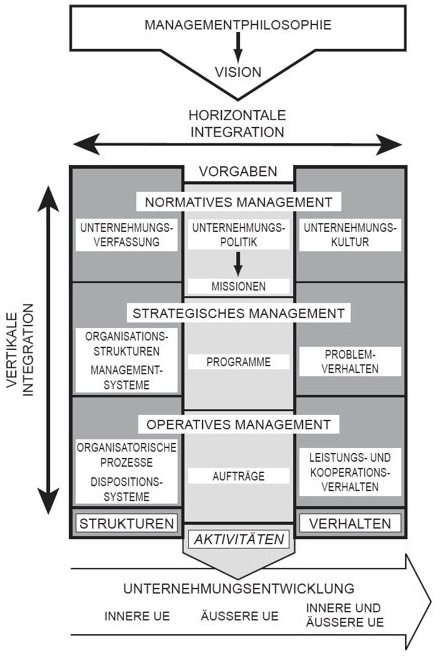
\includegraphics[width=0.75\linewidth,height=\textheight,keepaspectratio]{images/figure71.png} \hfill{}

\caption{Abb. 7.1: Das Konzept integriertes Management im St.~Galler
Managementmodell der zweiten Generation (Bleicher, 1999, S. 77, 82)}

\end{figure}%

Im Modell erfolgt zusätzlich eine horizontale und vertikale Integration:
Wie in der Abbildung zu sehen ist, geht das Modell von einer
Koordination zwischen Strukturbildung, Prozessumsetzung und Verhalten
der Mitarbeitenden zur Gestaltung der Zusammenarbeit aus (horizontale
Integration) als auch von einer hierarchisch organisierten
Top-Down-Strategie (vertikale Integration). Wie der Pfeil im unteren
Teil der Grafik zeigt, ist die Abstimmung zwischen den Managementebenen
grundsätzlich in einen Prozess der Unternehmensentwicklung einbettet. Es
wird von einer Veränderlichkeit und Dynamik ausgegangen und Anpassungen
an die jeweils veränderten Rahmenbedingungen sind an der Tagesordnung.

Alle drei Ebenen helfen uns dabei, die verschiedenen Aufgaben im Alltag
von Organisationen besser zu strukturieren, Verantwortlichkeiten zu
definieren und die Zusammenarbeit zu koordinieren. Kurz zusammengefasst
geht es auf normativer Ebene darum: Warum tun wir die Dinge, die wir
tun? Auf strategischer Ebene geht es um die Frage: An welchen konkreten
Zielsetzungen richten wir unsere Arbeit aus? Und auf operativer Ebene
geht es darum: Welche Aufträge haben wir heute zu erledigen, die am Ende
der geplanten Wirtschaftsperiode dahingehend überprüft werden müssen, ob
die gesetzten Ziele erreicht worden sind und ob wir dem
Unternehmenszweck besser gerecht geworden sind?

\subsection{St.~Galler Management Modell der dritten
Generation}\label{st-galler-management-modell-der-dritten-generation}

Da die dritte Generation des St.~Galler Management-Modells bereits
weiter oben ausführlich beschrieben wurde, soll an dieser Stelle nur ein
kurzer Überblick gegeben werden. In diesem Modell gibt es zunächst die
äußeren Umweltsphären Gesellschaft, Natur, Technologie und Wirtschaft.
Darüber hinaus wird sich auf den inneren Sphären, den
Interaktionsthemen, über Ressourcen, Werte, Anliegen und Interessen
ausgetauscht. Beide Aspekte gehören zur Systemumwelt. Auf den äußeren
Schalen sind die Stakeholder angesiedelt, die in Interaktion zwischen
der Systemumwelt und der Organisation stehen. Dazu zählen
unterschiedliche Akteure, Gruppen und Personen. Im Zentrum des Modells
steht die Unternehmung mit den verschiedenen Prozessstrukturen und
Ordnungsmomenten (Strategien, Strukturen und Kultur). Die Organisation
befindet sich in einem ständigen Entwicklungsprozess (Pfeilspitzen) im
Rahmen von entweder Erneuerungs- oder Optimierungsprozessen (erste und
zweite Ordnung) (vgl. \hyperref[figure72]{Abb. 7.2} nach Rüegg-Stürm,
2003).

\begin{figure}

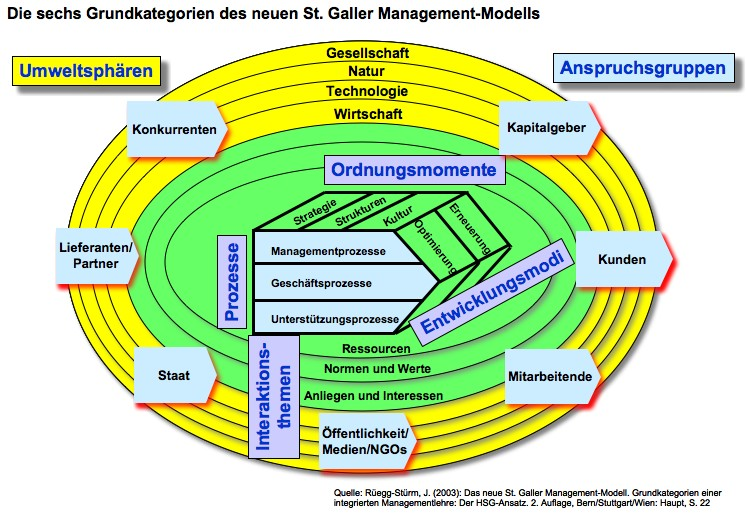
\includegraphics[width=0.75\linewidth,height=\textheight,keepaspectratio]{images/figure72.jpeg} \hfill{}

\caption{Abb. 7.2: Grundkategorien des SGMM (Rüegg-Stürm, 2003, S. 22),
Quelle: \url{https://de.wikipedia.org/wiki/Datei:SGMM2.jpg} (CC Public
Domain)}

\end{figure}%

Das gesamte Modell ist relativ übersichtlich gestaltet und gibt einen
Orientierungsrahmen vor, wie das organisationsbezogene Management
umgesetzt werden kann. Es stellt eine Ressource bzw. Rahmenplan dafür
dar, worauf im Management zu achten ist. Nachteilhaft in der Darstellung
könnte \emph{erstens} sein, dass die einzelnen Managementaufgaben nicht
explizit beschrieben werden. \emph{Zweitens} wird in diesem Modell nicht
explizit das Personalmanagement, Personalentwicklungsprozesse,
Personalführungsprozesse oder Personalmotivation betont. All diese
Aspekte spielen bei der Zusammenarbeit in Organisationen eine wichtige
Rolle. Dies ist in dem Sinne kein blinder Fleck, aber diese Aspekte sind
im Modell noch nicht intensiv genug mitgedacht. Sie lassen sich aber
integrieren, wenn man das Personalmanagement zu den Managementprozessen
hinzuzählt. Nichtdestotrotz ist die Personal- und
Organisationsentwicklung heutzutage untrennbar miteinander verbunden und
das muss in den allgemeinen Management-Modellen mitberücksichtigt
werden. Im Vergleich zur vierten Generation fehlt in diesem Modell
\emph{drittens} noch die integrative Sichtweise von Management als
kollektive Praxis. Bereits in der ersten Generation ist in den äußeren
Schalen eine Stakeholder-Sichtweise bereits integriert, nur dass dort
das Unternehmen noch nicht so differenziert dargestellt wird wie in der
dritten Generation. \emph{Viertens} lässt sich die zweite Generation nur
teilweise auf der prozessualen Ebene erkennen, wenn zwischen
Managementprozessen (strategische Ebene) und Geschäfts- und
Unterstützungsprozessen (operative Ebene) unterschieden wird. Mit
Geschäftsprozessen sind die Alltagsaufgaben (z. B. Gruppendienste,
Betreuungs- und Beratungsaufgaben) gemeint. Die Unterstützungsprozesse
beinhalten alltägliche Aufgaben unterstützende Dienste wie z. B.
Essensversorgung, Reinigungsdienste und Hausmeisterdienste. Kurz
zusammengefasst handelt es sich um ein ganzheitliches Management-Modell,
was uns die Organisation aus der Vogelperspektive zu betrachten erlaubt
und die Systemumwelt einbezieht.

\section{Non-Profit-Modelle}\label{non-profit-modelle}

\subsection{Freiburger Management-Modell für
Non-Profit-Organisationen}\label{freiburger-management-modell-fr-non-profit-organisationen}

Das Freiburger Management-Modell wurde vorrangig im Rahmen von Lehrenden
in einem Masterstudiengang für Non-Profit-Management an der Universität
Freiburg entwickelt und ist sehr an die Praxis angelehnt. Anwendbar ist
dieses Modell insbesondere auf gemeinnützige Organisationen, Verbände,
Vereine, Stiftungen etc. Es handelt sich um ein systemtheoretisches
Management-Modell, wobei einerseits erfolgskritische Einflussfaktoren
auf Managemententscheidung betrachtet werden und andererseits die
Gestaltung und Umsetzung des Non-Profit-Managements in Organisation im
Vordergrund steht (vgl. \hyperref[figure73]{Abb. 7.3} nach Schwarz et
al., 1999, S. 34).

\begin{figure}

\pandocbounded{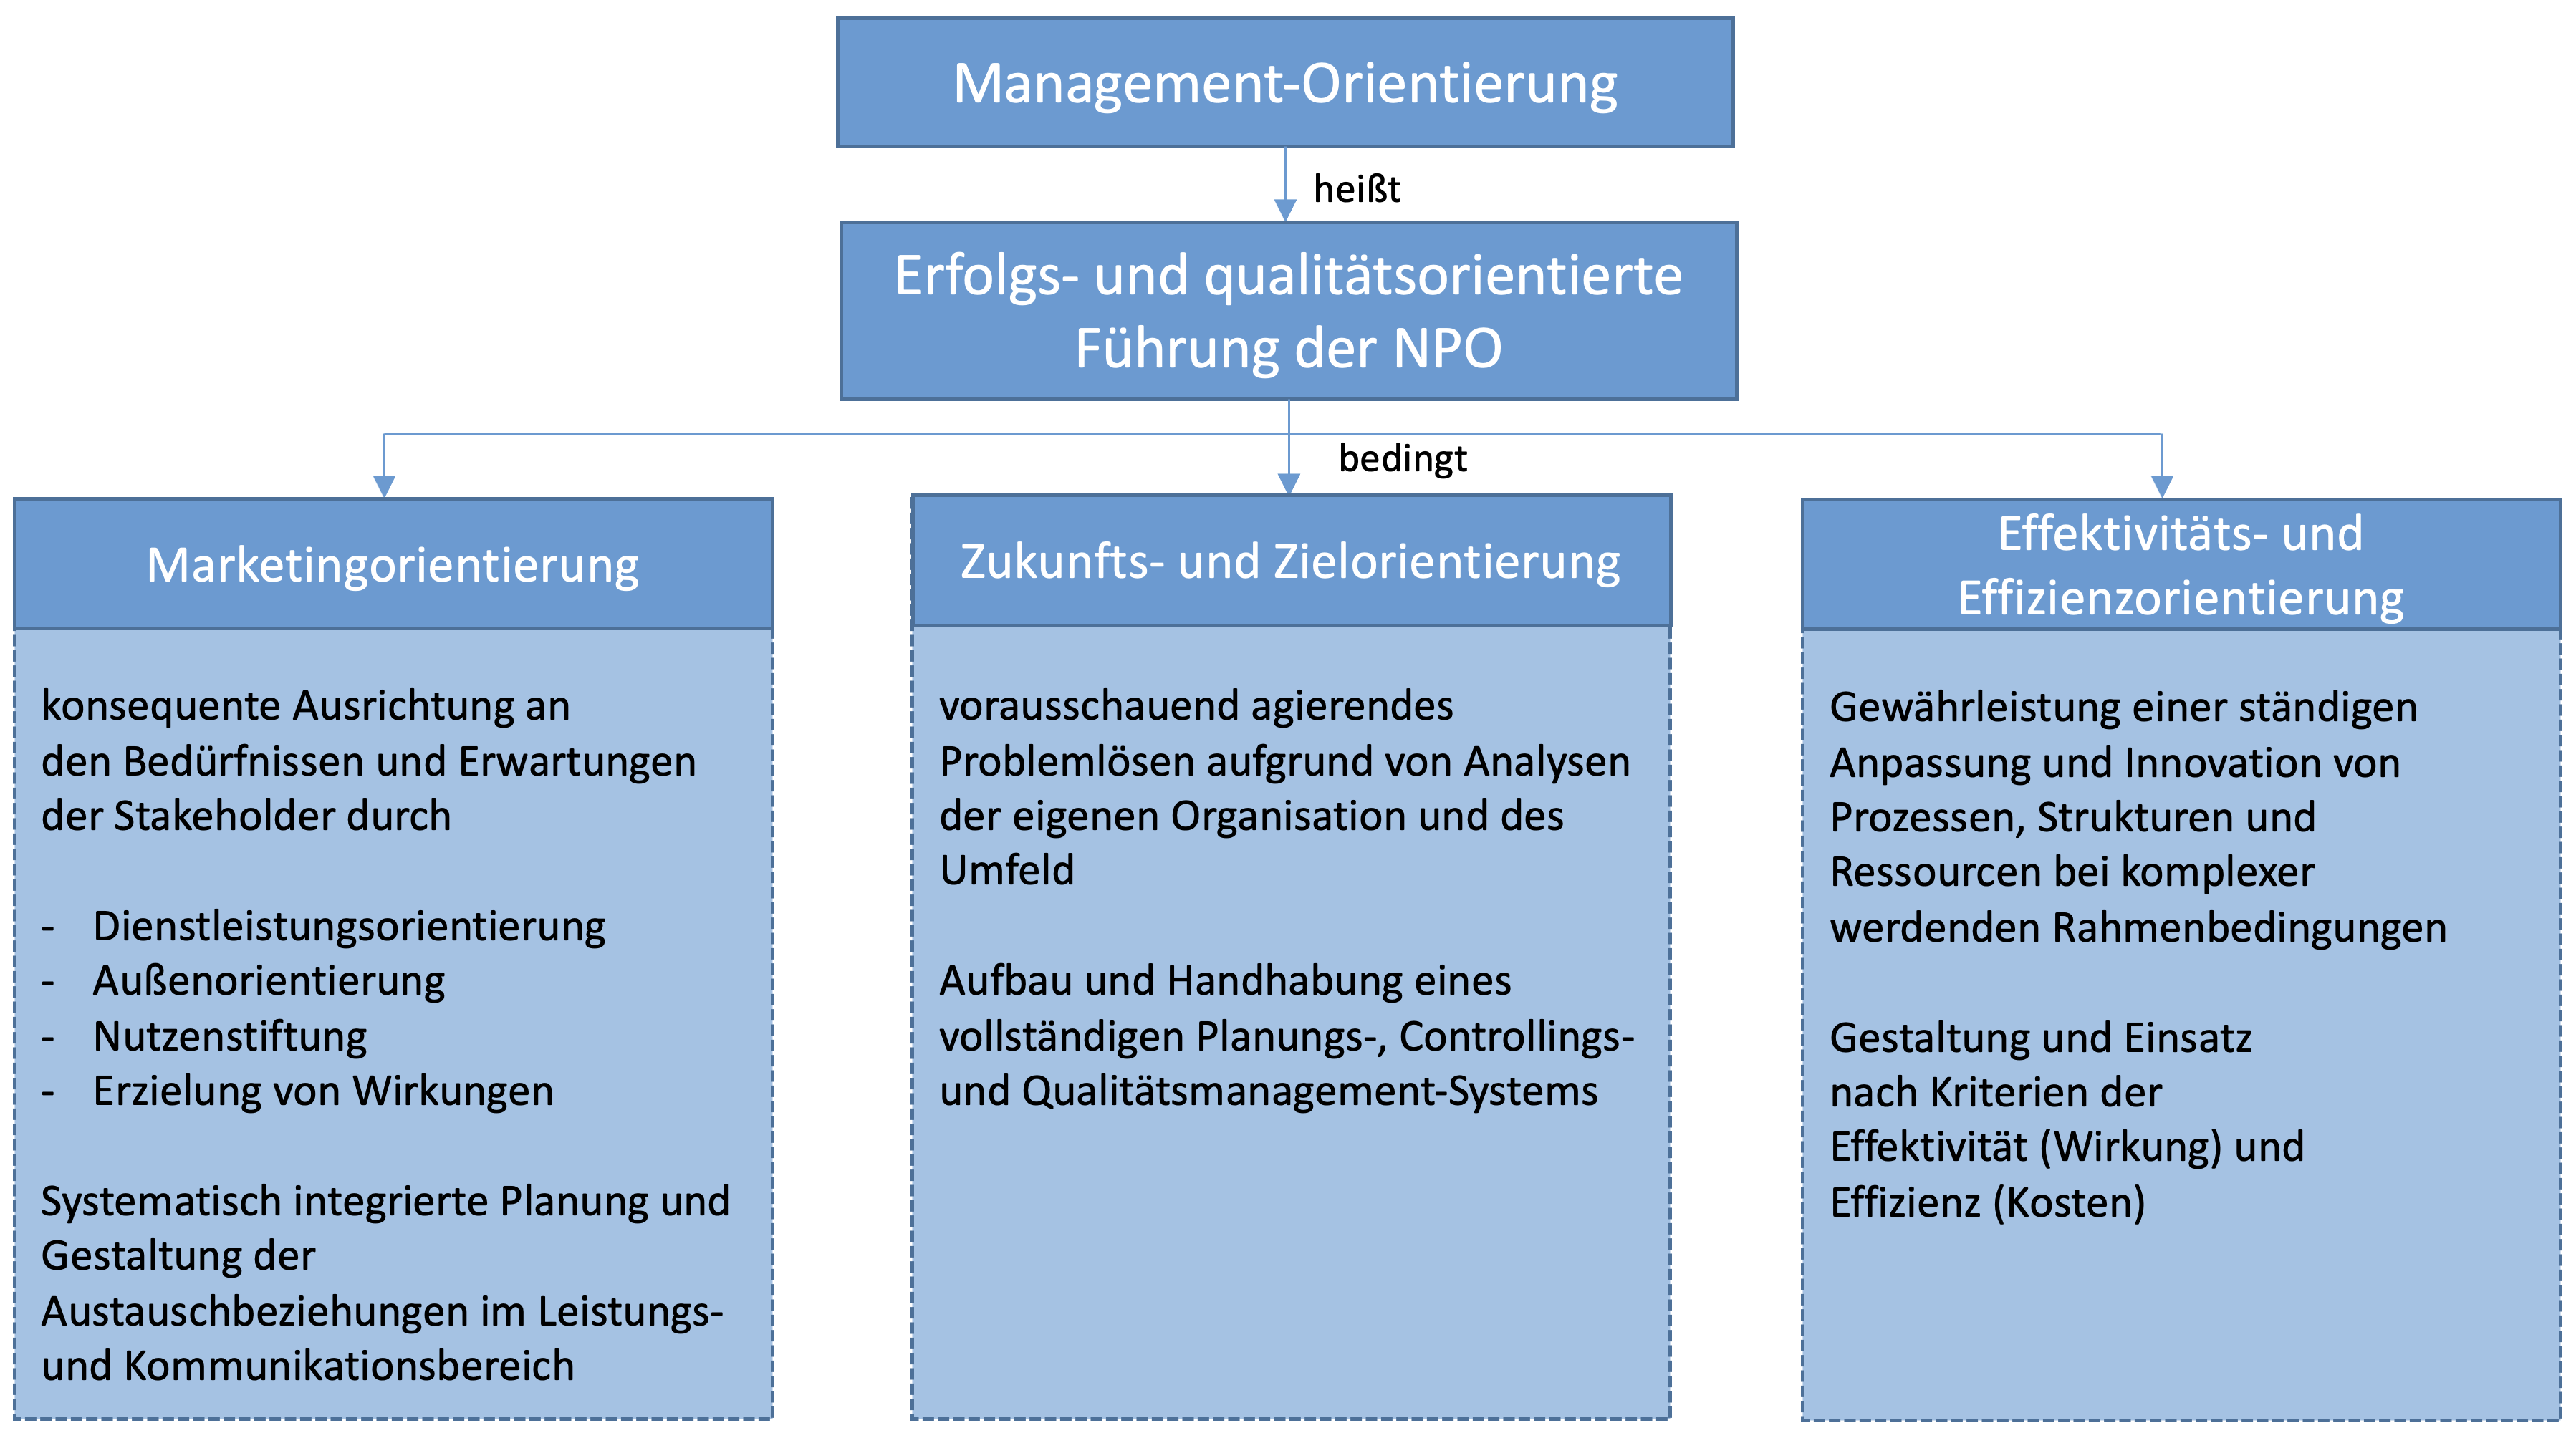
\includegraphics[keepaspectratio]{images/figure73.png}} \hfill{}

\caption{Abb. 7.3: Freiburger Management-Modell (nach Schwarz et al.,
1999, S. 34)}

\end{figure}%

Es wird visualisiert, welche Funktionsbereiche innerhalb einer
gemeinnützigen Organisation von Bedeutung sind. Zum besseren Verständnis
kann man sich als Hintergrundfolie eine \emph{Stiftung als
Non-Profit-Organisation} vorstellen, die unter Verwendung der Erträge
ihres Vermögens (Kapitalstock) die Begünstigten hinsichtlich eines
festgelegten Zwecks unterstützt bzw. fördert. Das Besondere von
Stiftungen ist, dass diese meist Aufgaben- und Zielstellungen verfolgen,
die keine private oder staatliche Organisation in dieser Form erfüllen
kann. Sie stellen mithin eine Ergänzung zur Verfolgung verschiedener
gesellschaftlicher Aufgaben dar und stärken die Zivilgesellschaft. Mit
dem Modell lassen sich sehr gut die Zweckverfolgung einer
Non-Profit-Organisation und die Nutzenstiftung bei den Begünstigten
nachverfolgen.

Das Modell vereint drei prinzipielle Zielsetzungen (sog.
„Orientierungen''), zu denen die Marketingorientierung, Zukunfts- und
Zielorientierung sowie Effizienz- und Effektivitätsorientierung gehören.
Das gesamte Management von Non-Profit-Organisationen soll auf diese drei
Perspektiven ausgerichtet werden, sodass sowohl \emph{erfolgs- als auch
qualitätskritische Aspekte} fokussiert werden können. Die Perspektive
der Zukunfts- und Zielorientierung betont die strategische Perspektive,
die Effektivität und Effizienzorientierung schaut auf die verfügbare und
zu entwickelnden Ressourcen und die Marketingorientierung weist darauf
hin, dass alles organisationale Handeln auf die Bedürfnisse der
Zielgruppe(n), Nutzer*innen der Leistungen, allgemein auf die
Stakeholder und Interessensgruppen der Einrichtung ausgerichtet werden
muss. Letztlich wird bei der \emph{Marketingorientierung} danach
gefragt, wie ein konsequentes Stakeholdermanagement umgesetzt werden
kann. Marketing bedeutet hier nicht einfach nur die Umsetzung der
Öffentlichkeitsarbeit, sondern es geht vielmehr darum, eine konsequente
Kund*innen- und Klient*innensicht einzunehmen (verschiedentlich auch als
Customer-Relationship-Management bezeichnet). Dabei ist danach zu
fragen, welche Dienstleistungen genau angeboten werden, welche Angebote
wie an die Adressaten gebracht werden, welcher Nutzen gestiftet werden
soll und welche Wirkungen erzielt werden sollen. Mit anderen Worten soll
eine konsequent systematische Sichtweise auf das Marketing eingenommen
werden. Eine Gestaltung der notwendigen Strukturen und Prozesse zwischen
dem Innen und Außen der Organisation sowie für die verschiedenen
Stakeholder verfolgt die Aufgabe der \emph{Zukunfts- und
Zielorientierung}. Hierbei geht es um die Frage, welche (Teil-)Aufgaben
in unserer Einrichtung organisiert werden müssen. Mit anderen Worten
handelt es sich hierbei um das „Systemmanagement'' zur strategischen
Steuerung der Einrichtung und von Entscheidungsprozessen, wobei solche
Fragen im Vordergrund stehen wie z. B. wie müssen unsere Einrichtung und
auch das Zusammenspiel mit dem Systemumfeld organisieren sollen, um dem
Einrichtungszweck bzw. grundlegenden Aufgaben nachzukommen bzw. gerecht
zu werden (vgl. Marketingorientierung oben). Zu den grundlegenden
Aufgaben einer Organisation zählen u. a. das Planungswesen, das
Controlling, das Personalmanagement, das Qualitätsmanagement. Neben der
Marketing- und der Systemperspektive gibt es noch die
Ressourcenperspektive, was in dem Modell mit der \emph{Effektivität- und
Effizienzorientierung} überschrieben wird. Hierbei geht es um die
Gewährleistung von Planungsprozessen, notwendiger Struktur und
verfügbarer (Finanz-)Mittel zum Betrieb der Einrichtung.
Prozessbeschreibungen und Organigramme müssen erstellt ~und/oder ein
Qualitätsmanagementhandbuch geschrieben werden, um, wie oben bereits
betont, dem Auftrag der Einrichtung gerecht zu werden. Es geht um die
Erfüllung der gesetzten strategischen Zielsetzungen mit Hilfe der zur
Verfügung stehenden materiellen, personalen, finanziellen und anderen
Ressourcen. Die Ressourceneinsatz sollte effizient und effektiv
gestaltet werden. Ebenso muss danach gefragt werden, welche Wirkungen
wir erzielt haben, gegenüber der Zielgruppe, bezogen auf die
Organisation, im Stadtteil bzw. allgemein für das Gemeinwohl.
Letztgenannte Sichtweise geht über die (finanztechnische)
Gewinnermittlung am Ende des Wirtschaftsjahres weit hinaus. Aus
Perspektive einer Stiftung müssen wir uns am Ende des Jahres u. a. die
Fragen stellen, welche Förderungen ermöglicht wurden und welche
gesellschaftlichen Veränderungsprozesse im Kleinen wie im Großen
angeregt wurden.

\subsection{Darmstädter
Management-Modell}\label{darmstdter-management-modell}

Ebenfalls aus der Non-Profit-Managementlehre stammt das Darmstädter
Management-Modell, welches stärker Bezug zum Sozialmanagement bzw. dem
Management von sozialen Organisationen nimmt. Dass das Modell aus einem
pädagogischen Kontext stammt, lässt sich anhand seiner Bestandteile
schnell erkennen, die auf konkrete Wissens- und Kompetenzbereiche, über
die eine Führungskraft im Management einer sozialen Organisation
verfügen sollte, hinweist.

Das Modell (vgl. \hyperref[figure74]{Abb. 7.4}) geht davon aus, dass
sich die Sozialwirtschaft in einem ständigen dynamischen Wandel befindet
und Sozialbetriebe sich häufig in einem sich kontinuierlich verändernden
Umfeld befinden. Solche Veränderung können sich aufgrund von
Gesetzesänderung, veränderte Klient*innenbedarfe etc. ergeben (vgl.
Fröse, 2005, S. 387).

\begin{figure}

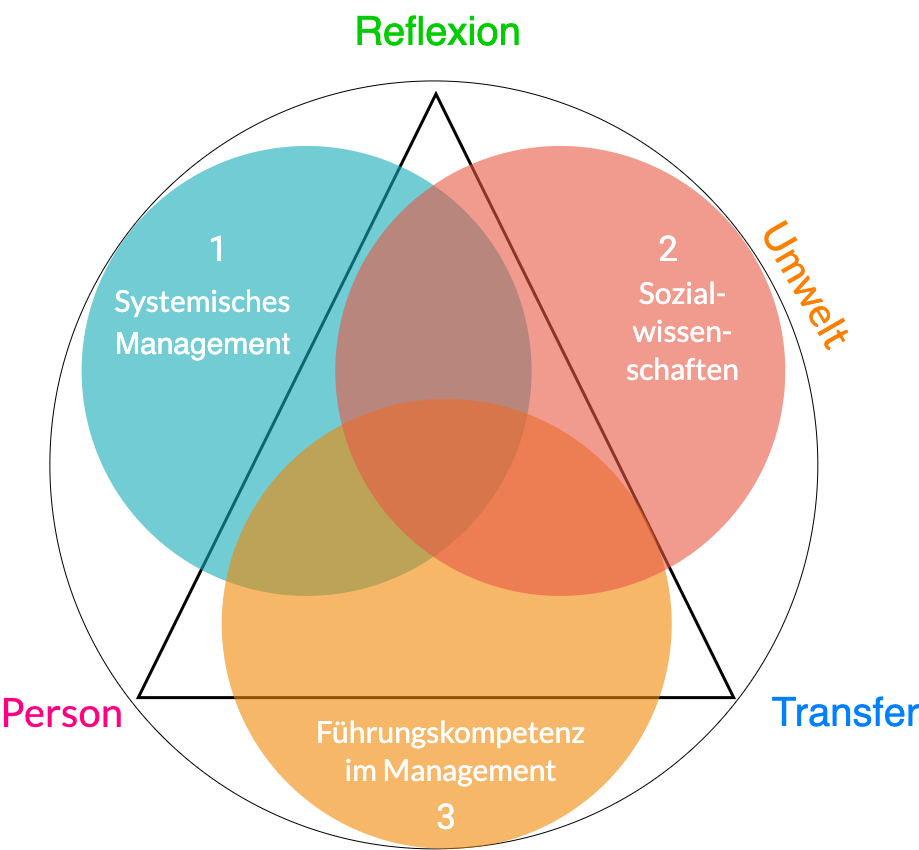
\includegraphics[width=0.75\linewidth,height=\textheight,keepaspectratio]{images/figure74.png} \hfill{}

\caption{Abb. 7.4: Darmstädter Management-Modell (in Anlehnung an Fröse,
2005, S. 387)}

\end{figure}%

Außerdem sind soziale Einrichtungen in den letzten Jahren in
verschiedenen Bereichen (z. B. Beratungen) damit konfrontiert, dass die
mit dem Leistungsträger hart verhandelten Leistungsentgelte häufig nicht
ausreichend sind, um alle entstehenden Aufwendungen zur
Leistungserbringung zu refinanzieren und sich eines Mix
unterschiedlicher Finanzierungsquellen bedienen müssen. Das Modell soll
schließlich das ganzheitlich-systemische Denken, Interdisziplinarität
und das interprofessionelle Lernen fördern. Dabei wird darauf geachtet,
dass einerseits die sozialarbeiterischen Kontexte und Bedingungen sowie
Hintergründe und Theorien einbezogen, andererseits aber auch die
wirtschaftlichen Rahmenbedingungen integriert werden. Zum Grundwissen
gehört beispielsweise Wissen über die Organisationsentwicklung,
Institutionenökonomik (Analyse der Wechselwirkungen von Wirtschaft und
gesellschaftlichen Institutionen, wie z. B. Entscheidungsprozesse,
Auftraggeber-Auftragnehmer-Verhältnisse) sowie Betriebs- und
Volkswirtschaftslehre und rechtliche Grundlagen.

Im äußeren Kreis des Modells finden sich die Hauptthemen, mit denen man
sich im Sozialmanagement-Studium beschäftigen sollte. Anders formuliert
handelt es sich um die Fähigkeiten und Kompetenzen, die relevant für
eine Führungskraft in sozialen Einrichtungen sind. Unten links steht das
Thema, die \emph{Persönlichkeit der Leistungskraft} und die Reflexion
des eigenen Leitungsstils. Oben steht die \emph{(Praxis-)Organisation}
mit den verschiedenen Funktionsbereichen sowie Organisationsentwicklung.
Rechts stehen \emph{Wissenschaft, Theorieperspektiven und
Analysetechniken}. Im Inneren des Kreises befinden sich drei aneinander
liegende Dreiecke (flächig betrachtet) bzw. eine Pyramide (räumlich
betrachtet). Ausgehend von den Kernthemen in den drei Ecken finden sich
drei Teilbereiche (nummeriert). Im ersten Bereich sind Kenntnisse über
\emph{Theorien und Praxis des systemischen Managements} abgebildet.
Diesem Themenfeld sind Grundlagen des Managements und der
Organisationsentwicklung sowie Reflexion der Managementpraxis in der
Gesellschaft (z. B. ethische Verantwortung und Veränderungen in der
Organisation und im Umfeld) zugeordnet. Im zweiten Teilbereich finden
sich die \emph{sozialwissenschaftlichen Grundlagen}, wozu u. a. das
Gesellschafts- und Steuerrecht, die Reflexion von Markt und Gesellschaft
(= Wahrnehmung des gesellschaftlichen Auftrags durch soziale
Einrichtungen), betriebswirtschaftliche Grundlagen für die Soziale
Arbeit, Arbeitsrecht und Forschungsmethoden gehören. Grundsätzlich sind
in diesem Teilbereich die interdisziplinären Grundlagen der Sozial-,
Rechts- und Gesellschaftswissenschaften zu finden. Im dritten
Teilbereich sind die \emph{Führungskompetenzen für das strategische
Management} von Einrichtungen abgebildet, wie z. B. Strategieplanung und
-überprüfung, das Verfolgen von internationalen Entwicklungen (z. B.
Migrations- und Flüchtlingshilfe sowie damit verbundene
Herausforderungen) sowie kulturelle und politische Entwicklungen und
Netzwerkarbeit.

Im Modell werden alle vorgenannten Kompetenz- und Wissensbereiche
abgebildet, nach denen entsprechend die Führungskräfte im Darmstädter
Studiengang an der Evangelischen Hochschule in Darmstadt ausgebildet
werden. Ähnlich wie beim St.~Galler Management-Modell geht es auch im
Darmstädter Management-Modell um wesentliche Grundlagen, Arbeitsfelder
und Funktionsbereiche des Managements in der Sozialwirtschaft. Eine
Spezialität des Modells ist, dass hier vordergründig das Kompetenzprofil
von einer idealtypischen Führungskraft betrachtet wird.

\subsection{Bielefelder
Diakonie-Management-Modell}\label{bielefelder-diakonie-management-modell}

Das Bielefelder Management-Modell kann sowohl in die
Non-Profit-Managementlehre als auch in die Diakoniewissenschaften
eingeordnet werden. Beide Disziplinen besitzen Anknüpfungspunkte in der
Beschäftigung mit Konzepten und Ansätzen zur Führung und zum Management
von Non-Profit-Organisationen. Die Diakoniewissenschaften beziehen sich
im Allgemeinen auch auf die betriebswirtschaftlichen Grundlagen für
Einrichtungen in konfessioneller Trägerschaft. Das Bielefelder Modell
knüpft unmittelbar am St.~Galler Management-Modell der zweiten
Generation, wie in \hyperref[figure75]{Abb. 7.5} in den drei Ebenen
normatives, strategisches und operatives Management leicht zu erkennen
ist. Auf der normativen Ebene geht es um die Ordnung der
Unternehmenspolitik, also die Festlegung des Zwecks der Einrichtung, der
Aufgabenfelder und Leistungsbereiche. Auf der strategischen Ebene geht
es darum, diese Grundsätze und Prinzipien in einen geeigneten
Planungsprozess zu überführen, Ziele zu setzen und Strategien zu
formulieren. Von Belang ist dabei die Erarbeitung und Überprüfung von
Vorgaben für den jeweiligen Planungszeitraum (z. B. sechs Monate, ein
oder mehrere Jahre). Und auf der operativen Ebene geht es um die
konkrete Unternehmensorganisation und die Umsetzung der
Managementaufgaben, die sich im Alltag stellen (vgl. Lohmann, 1997).

\begin{figure}

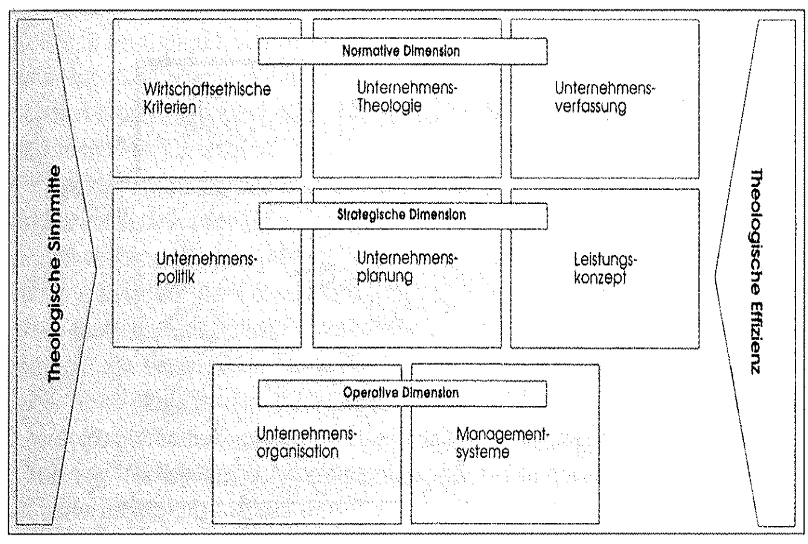
\includegraphics[width=0.75\linewidth,height=\textheight,keepaspectratio]{images/figure75.png} \hfill{}

\caption{Abb. 7.5: Bielefelder Diakonie-Management-Modell: Dimensionen
(Lohmann, 1997, S. 172)}

\end{figure}%

Diese drei Ebenen werden schließlich von der theologischen Sinnmitte
(links) und der theologischen Effizienz (rechts) flankiert. Mit
\emph{theologischer Sinnmitte} ist gemeint, dass alle theologischen
Fragestellungen, die sich durch Entscheidungsprozesse im Management
tagtäglich ergeben, genauer als wirtschaftsethische Fragestellungen zu
reflektieren sind. Mit anderen Worten gibt es immer eine zweite
Komponente, die bei Entscheidungen und der Umsetzung von Aufgaben
mitgedacht werden muss, nämlich die wirtschaftsethische Reflexion des
eigenen ökonomischen Handelns, was z. B. in ethischen Fallbesprechung
umgesetzt werden kann. Reflektiert werden sollte nach dieser Ansicht,
wie mit Verantwortung umgegangen worden ist, wie Lösung für
Dilemmasituationen gefunden werden können und wie mit den Mitarbeitenden
umgegangen wurde. Mithin wird hervorgehoben, dass diese ethische
Reflexionsfähigkeit eine wichtige Führungskompetenz darstellt. Unter
\emph{theologischer Effizienz} wird verstanden, dass die Effizienzfrage
im wirtschaftlichen Handeln erweitert werden muss. Natürlich haben
konfessionelle Träger die gleichen ökonomischen Grundlagen und
Rahmenbedingungen wie andere soziale Einrichtungen. In diesem Modell
erfolgt eine Erweiterung um eine theologische Sichtweise, nach der es
immer wieder abzuwägen gilt, ob der diakonische Auftrag der Einrichtung
auch erreicht werden konnte oder wie man dem Auftrag zukünftig besser
gerecht werden kann. Beide Aspekte, die theologische Sinnmitte und die
Effizienz, fungieren allgemein als Reflexionsebene, die im Alltag von
konfessionellen Einrichtungen mitgedacht werden muss.
Institutionalisiert ist dieses Prinzip in der Praxis beispielsweise
dadurch, dass im Vorstand meist mindestens zwei Ressorts verteilt sind:
eine kaufmännische Geschäftsführung und im Regelfall zusätzlich noch die
theologische Geschäftsführung. Leitungsentscheidungen soll gleichzeitig
aus kaufmännischer und theologischer Perspektive abgewogen und nicht
gegeneinander ausgespielt werden.

\begin{figure}

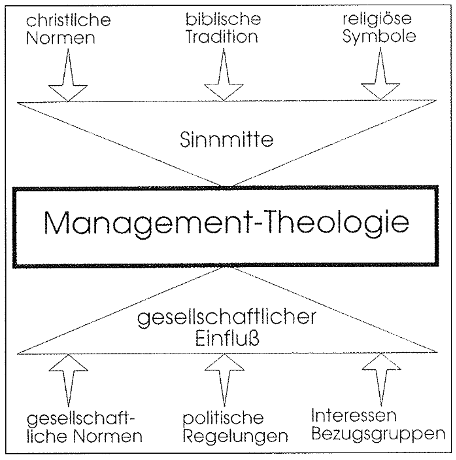
\includegraphics[width=0.6\linewidth,height=\textheight,keepaspectratio]{images/figure76.png} \hfill{}

\caption{Abb. 7.6: Bielefelder Diakonie-Management-Modell:
Management-Theologie (Lohmann, 1997, S. 190)}

\end{figure}%

In \hyperref[figure76]{Abb. 7.6} ist zur Verdeutlichung des
Verhältnisses von Management und Theologie eine Grafik abgebildet, die
diesen Aspekt noch einmal auf den Punkt bringt. Im Mittelpunkt des
Diakoniemanagements stehen -- wie bereits beschrieben -- sowohl
theologische als auch betriebswirtschaftliche Fragen, die wie zwei
Zahnräder ineinandergreifen müssen, da nur dann die Organisation
funktioniert. So sind immer die Beziehungen \emph{Management-Theologie}
und \emph{Theologie-Management} zu betrachten. Aus Perspektive der
theologischen Sinnmitte wird auf biblische, christliche, religiöse
Traditionen und Rituale zurückgegriffen (z. B. gemeinsame Gottesdienste,
Seelsorgeangebote für Mitarbeitende). Es sind aber auch die
gesellschaftlichen, politischen, ökonomischen und natürlichen
Rahmenbedingungen und Ressourcen unter Einbeziehung von Interessen der
Stakeholder zu beachten. Alles das hat Einfluss auf die Gestaltung des
Managements in der diakonischen Einrichtung und beeinflusst alle
Entscheidungen.

Im Rahmen dieses Kapitels wurden viele verschiedene Modelle beschrieben,
die ganz unterschiedliche Schwerpunkte setzen. Es gilt immer zu prüfen,
wie welche Modelle sich in welchen Kontexten und für welche
Einrichtungen anwenden bzw. auf diese übertragen lassen.

\chapter{Social Entrepreurship}\label{social-entrepreneurship}

Die Zahl der Existenzgründungen in Deutschland hat -- gemessen an den
Gewerbeanmeldungen und damit auch der Zahl der Gründer*innen -- in der
letzten Dekade in absoluten Zahlen stetig abgenommen. Im Jahr 2018
wurden knapp 542.500 Betriebe neu gegründet (Statistisches Bundesamt,
2019). Dieser Rückgang ist insbesondere bei Betrieben mit größerer
wirtschaftlicher Bedeutung und Kleinunternehmen zu beobachten. Die Zahl
der Nebenerwerbsbetriebe hat gegenüber Klein- und mittelständischen
Unternehmen leicht zugenommen. Zu ähnlichen Ergebnissen kommt auch das
Institut für Mittelstandsforschung Bonn (2021): Im Jahr 2018 wurden ca.
367.000 Existenzgründungen in Deutschland erfasst; 3,6 \% weniger als im
Vorjahr (vgl. \hyperref[figure81]{Abb. 8.1}). Davon entfielen 269.950
Gründungen auf den gewerblichen Bereich (73,5 \%), 90.380 (24,6 \%) auf
die freien Berufe und sonstige Selbständige sowie 6.720 (1,8 \%) auf den
Bereich der Land- und Forstwirtschaft. Im OECD-Vergleich lag Deutschland
im Jahr 2018 mit einer Selbständigkeitsquote von nur 9,9 \% der
Erwerbstätigen im unteren Feld (OECD, 2019, S. 60), während im
europäischen Vergleich die Selbständigkeitsquote 15,5 \% beträgt.

\begin{figure}

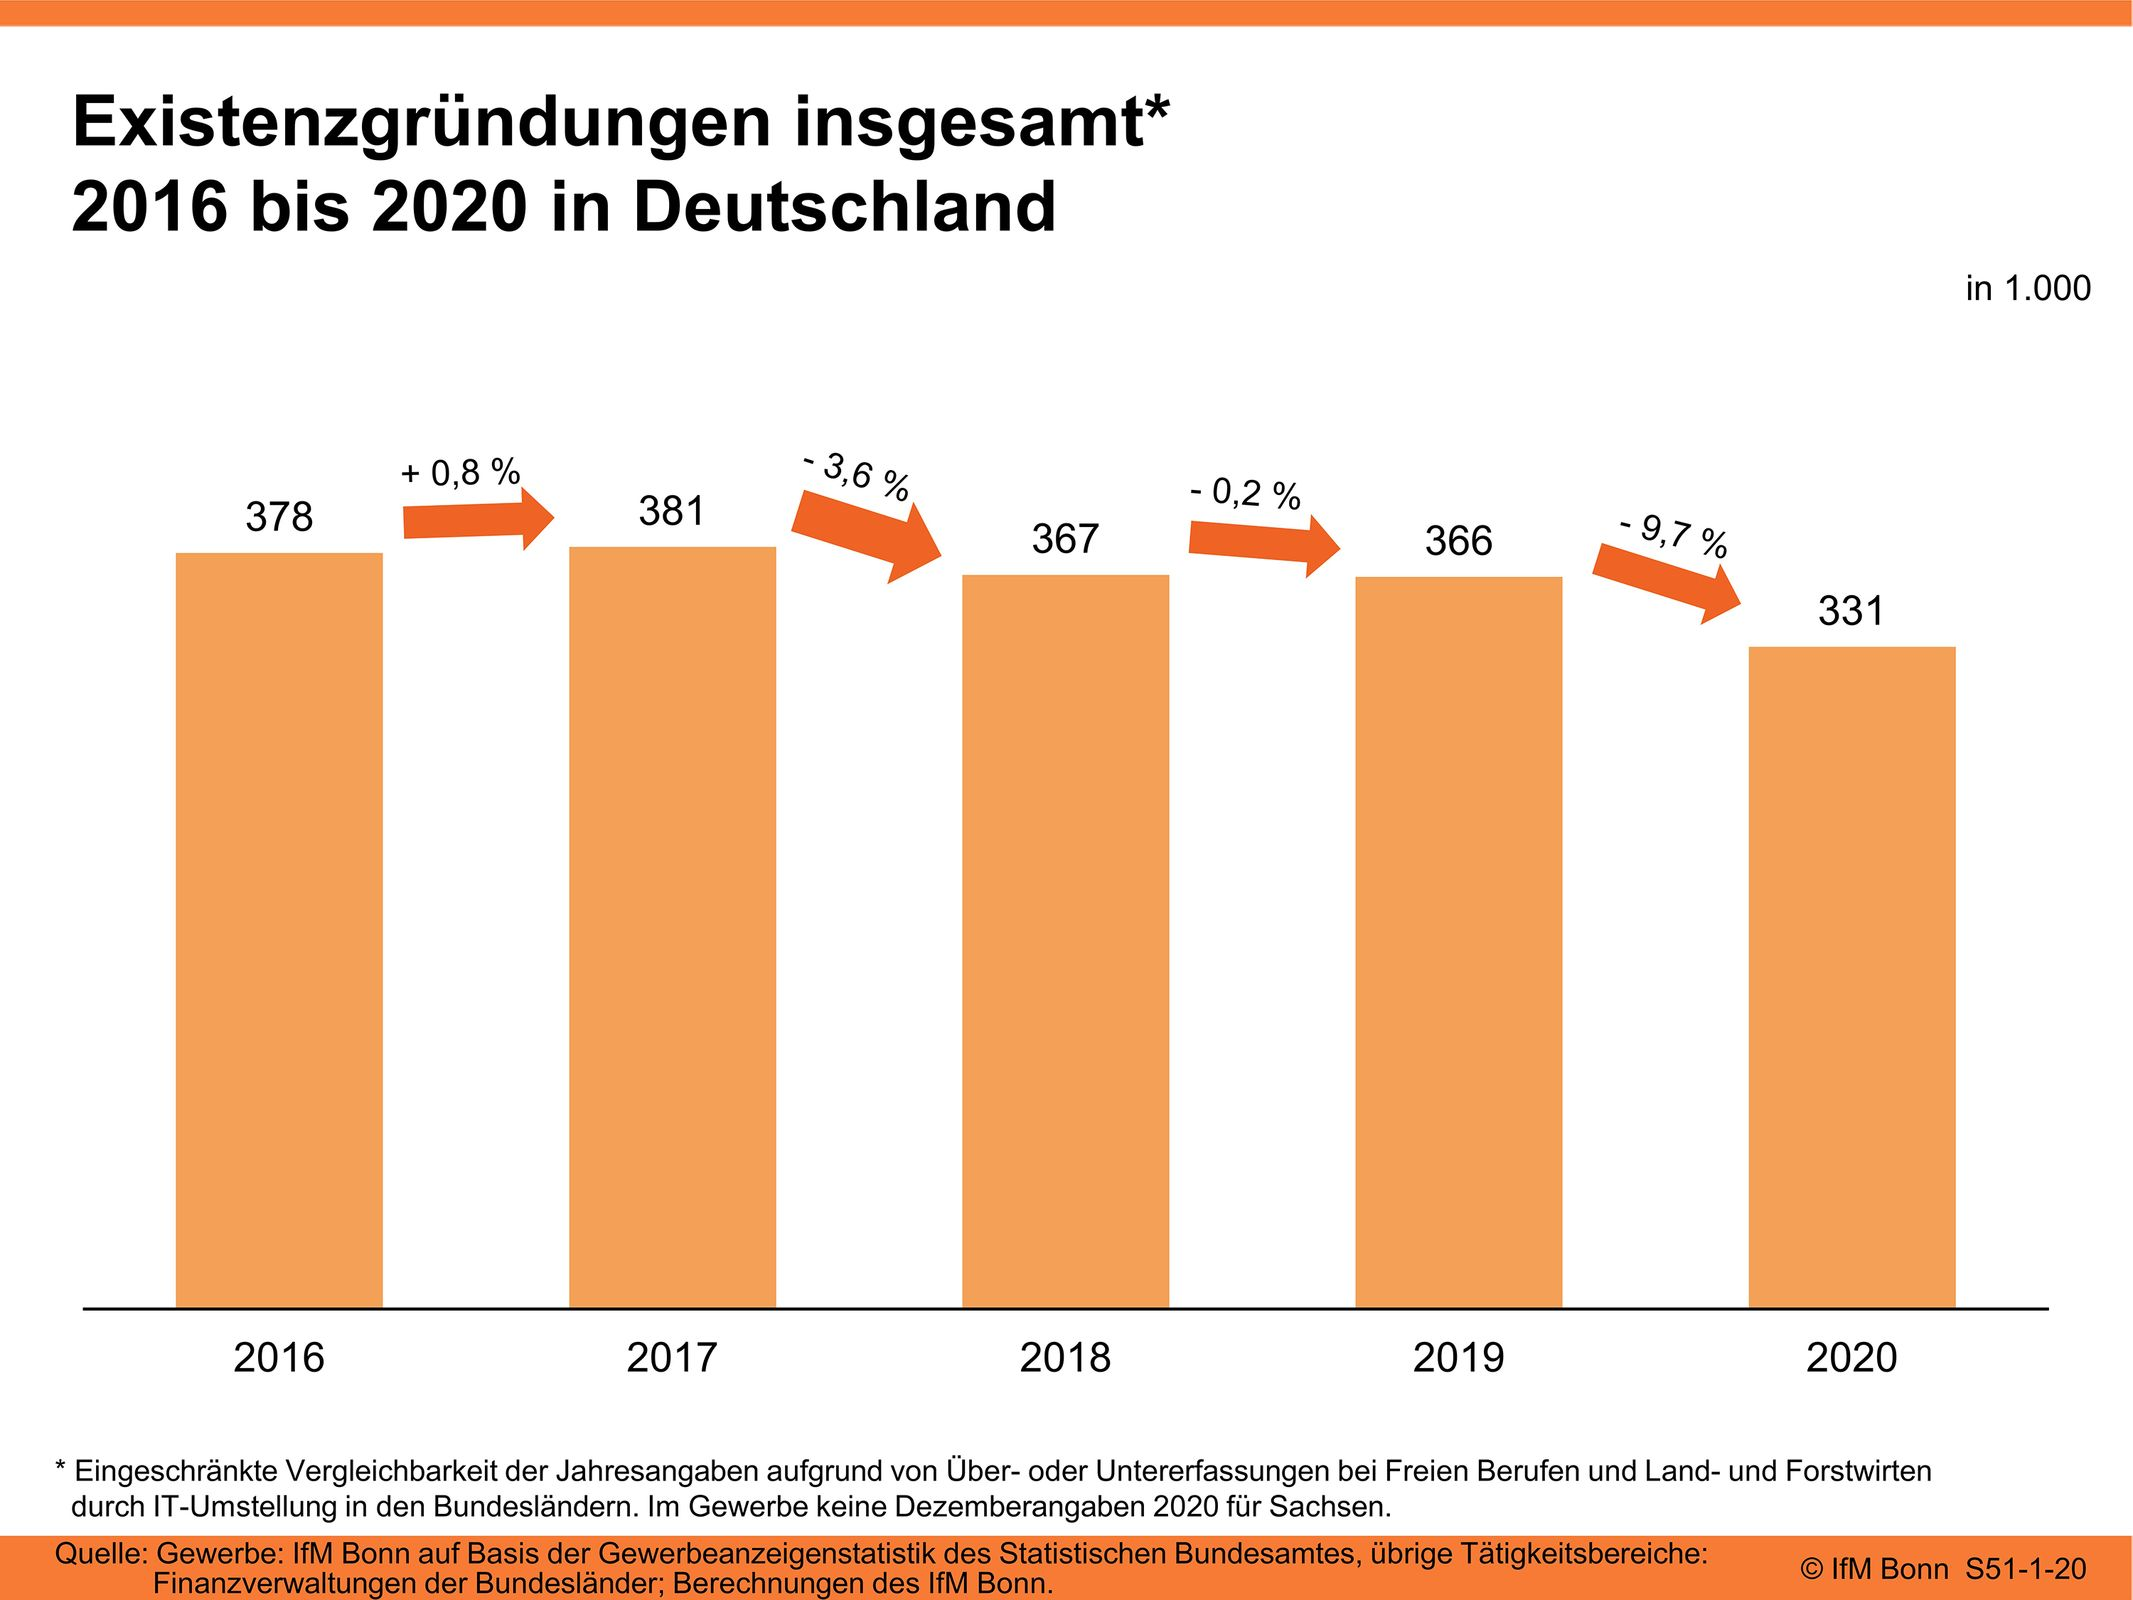
\includegraphics[width=0.75\linewidth,height=\textheight,keepaspectratio]{images/figure81.jpeg} \hfill{}

\caption{Abb. 8.1: Existenzgründungen insgesamt 2015-2019 in Deutschland
(Institut für Mittelstandsforschung Bonn, 2021, Quelle:
\url{https://www.ifm-bonn.org/fileadmin/data/redaktion/statistik/gruendungen-und-unternehmensschliessungen/bilder/S51-1-20.jpg})}

\end{figure}%

Zwar finden die meisten Existenzgründungen nach wie vor primär im
gewerblichen Sektor statt. Allerdings eröffnen sich zunehmend auch
Spielräume im sozial- und gesundheitswirtschaftlichen Sektor. Dies
geschieht einerseits durch Ausgliederung von Dienstleistungen
verschiedener Servicebereiche öffentlicher Einrichtungen (Outsourcing).
Andererseits ergeben sich aufgrund der kritisch beschworenen

„Ökonomisierung des Sozialen'' und aufgrund (quasi-)marktlicher
Strukturen und Marktmechanismen, die u. a. durch das Neue
Steuerungsmodell bewirkt werden, ein Spielraum für soziales
Unternehmertum. Nach dem Survey der ZiviZ GmbH (2017) verstehen sich
etwa 16 \% aller sozialen Einrichtungen als Sozialunternehmen. In
absoluten Zahlenausgedrückt handelt es sich dabei um ca. 80.000
gemeinnützige Organisationen (von insgesamt 634.000). Ein ähnliches
Ergebnis erbrachte auch der Deutsche Startup Monitor 2018 des
Bundesverband Deutsche Startups (2020): Ca. 42,6\% der befragten
Start-ups ordnen (im Vergleich zu 2019: 41,9\% und 2018: 38,7\%) das
gesellschaftliche Engagement ihres Unternehmens dem Sozialunternehmertum
zu. Im Rahmen einer aktuellen Untersuchung des Social Entrepreneurship
Netzwerk Deutschland e. V. (SEND) (2018) lassen sich eine Reihe
interessanter weiterer Erkenntnisse ableiten, die ein spezifisches Bild
von der aktuellen Situation für Sozialunternehmer zeichnen:

\begin{itemize}
\item
  9 von 10 Sozialunternehmen lösen gesellschaftliche Probleme in
  Deutschland; 3 von 4 sind dabei höchstinnovativ;
\item
  50 \% der Sozialunternehmen wurden von Frauen gegründet;
\item
  in 56 \% der Sozialunternehmen nehmen Mitarbeitende direkten Einfluss
  auf Entscheidungen bzw. haben ein Mitspracherecht;
\item
  33 \% der Sozialunternehmen bewerten die festgestellten Wirkungen und
  Effekte sowie angebotene Produkte und Dienstleistungen als weltweite
  oder EU-weite Marktneuheit;
\item
  62 \% der Befragten sehen in der Startfinanzierung und 65 \% in der
  Anschlussfinanzierung eine wesentlicheBarriere;
\item
  55 \% empfinden den Zugang zu Unterstützungsangeboten als wesentliche
  Hürde;
\item
  die Politik erhält lediglich die Note 4,6 auf einer Skala von 1 (sehr
  gut) bis 5 (schlecht) für die Unterstützung von Social
  Entrepreneurship in Deutschland;
\item
  73 \% der Sozialunternehmen wünschen sich eine stärkere Repräsentation
  und Anerkennung;
\item
  Sozialunternehmen sind nicht nur sehr heterogen, sondern sind auch in
  ihren Geschäfts- und Wirkungsmodellen, den gewählten Rechtsformen und
  der Finanzierung sehr vielseitig;
\item
  87 \% der Sozialunternehmen streben eine Skalierung ihres
  Geschäftsmodell an.
\end{itemize}

Die Ergebnisse der einführend genannten Studien zeigen, dass der
Neugründung von Einrichtungen der Sozial- und Gesundheitswirtschaft
innerhalb einer Volkswirtschaft eine große Bedeutung zukommt. Umso
wichtiger ist es, dieVoraussetzungen, Grundlagen und Rahmenbedingungen
zu kennen, die Gründer*innen einen Weg in dieSelbständigkeit im
Sozialsektor ermöglichen, um erfolgreich und nachhaltig innovative
Geschäftsideen umzusetzen.

\section{Existenzgründung in der
Sozialwirtschaft}\label{existenzgrndung-in-der-sozialwirtschaft}

\section{Unternehmerische Rahmenbedingungen in der
Sozialwirtschaft}\label{unternehmerische-rahmenbedingungen}

Aufgrund seiner historischen Wurzeln in den Bismarck'schen
Sozialgesetzen kommt dem deutschen Sozialstaatsmodell eine besondere
Bedeutung zu. Zu den Prinzipien der sozialen Sicherung und rechtlichen
Rahmenbedingungen zählen u. a. das Äquivalenzprinzip (nur diejenigen
erhalten Leistungen, die auch inVersicherungen eingezahlt haben, z. B.
gesetzliche Sozialversicherungen), Solidarprinzip (steuerfinanzierte
Entschädigungen, Förderungen und soziale Hilfen, z. B. Kriegsversehrte,
Kindergeld, Sozialhilfe) und Subsidiaritätsprinzip (vorrangige
Berücksichtigung von sozialen Wohlfahrtsträgern gegenüber öffentlichen
Leistungsträgern), um nur einige wenige zu nennen.

Vor diesem Hintergrund haben Sozialunternehmen im Wirtschaftskreislauf
eine besondere Stellung. Ihre indirekte Finanzierung erfolgt
grundsätzlich im Rahmen des sozialrechtlichen Dreiecksverhältnisses
zwischenSozialleistungsträger, Leistungsempfänger und
Leistungserbringer. Die Leistungsempfänger (die Hilfesuchenden)haben
Anspruch auf eine Leistung (z. B. Bildung und Betreuung von Kindern),
der Kostenträger (z. B. Jugendamt)gewährt diese und der
Leistungserbringer bzw. soziale Dienstleister (z. B. Kindertagesstätte)
erbringt bzw. organisiertdiese unmittelbar (Kolhoff, 2017, S. 5). Der
Leistungsträger erhält für die in den Sozialgesetzen definierten
Aufträge aus den vom Staat bereitgestellten Haushaltsmitteln (z. B.
Steuern und Sozialabgaben) eine Aufwands- bzw. Kostenentschädigung. Die
Finanzierung der Leistungserbringung erfolgt über Sach- oder
Geldleistungen indirekt an die die Leistungen erbringenden
Sozialunternehmen oder ggf. direkt an die Leistungsempfänger selbst (z.
B. persönliches Budget, Gutscheine, Selbstzahler). Um handlungsfähig zu
sein, müssen Sozialunternehmen bestimmte Produkte und Dienstleistungen
von anderen Unternehmen einkaufen (z. B. Büro- und Geschäftsausstattung,
Spielgeräte etc.) und rekrutieren Fachkräfte vom Arbeitsmarkt.

Die Finanzierung von sozialen Einrichtungen in freier Trägerschaft ist
letztlich durch einen Finanzierungsmix (auch Welfare-Mix; vgl. dazu
ausführlicher Abschnitt \hyperref[finanzierungsmix]{Finanzierungsmix für
freie Träger der Wohlfahrtspflege} geprägt: Neben den Leistungsentgelten
vom Kostenträger (indirekte Subjektfinanzierung) oder öffentlichen
Zuwendungen bzw. Zuschüssen(Objektfinanzierung; z. B. über Projekt- oder
institutionelle Förderung) müssen diese ihren Finanzierungsbedarf immer
öfter auch aus nicht öffentlichen Mitteln bestreiten wie z. B.
Stiftungsgelder, Spenden, Elternbeiträge, Vereinsbeiträge und ggf. auch
kirchlichen Zuwendungen. Weiterhin spielen das Sponsoring oder andere
Fundraising-Aktivitäten eine wichtige Rolle. Aus
betriebswirtschaftlicher Sicht sind schließlich die Selbstfinanzierung
durch Überschüsse aus erwirtschafteten Gewinnen, Vermögensumschichtungen
etc. mit zu bedenken. In den letzten Jahren hat insbesondere die
Finanzierung von Initiativen, Projekten und Ideen mithilfe
desCrowdfundings an Bedeutung zugenommen (vgl. ausführlicher in
Abschnitt \hyperref[finanzierung-sozialwirtschaft]{Finanzierung in der
Sozialwirtschaft}. Sozialunternehmen sind bei ihrer Finanzierung auf
einen Mix an verschiedenen Finanzierungsquellen angewiesen, was als
\emph{Welfare-Mix }bezeichnet wird.

Aufgrund dieser Rahmenbedingungen ist es für gewerbliche Einrichtungen
schwieriger, in der Sozialwirtschaft tätig zu werden. Dies ist nur
begrenzt und in einzelnen Nischen möglich, wie z. B. in der
Raumvermietung fürstationäre Einrichtungen. Existenzgründungen werden in
der Sozialwirtschaft insbesondere durch freiberuflich Tätige initiiert,
z. B. soziale, therapeutische Beratungen oder pädagogische Tätigkeiten,
die auf Honorarbasis fürgemeinnützige freie Träger tätig werden. Ein
Grund dafür ist, dass es aufgrund des deutschen Sozialstaatsmodells
imZusammenspiel zwischen sozialem und erwerbswirtschaftlichem Sektor zur
Herausbildung sog. „kollusiver Strukturen'' (Kolhoff, 2002, S. 22-24)
gekommen ist. Unter~ \emph{Kollusion }(lat.~ \emph{colludere},~
zusammenspielen) des~ sozialen~ Sektors versteht~man den Umstand, dass
der Staat eine progressive und die Soziale Arbeit eine regressive
Funktion übernimmt.

Im einfachsten Fall entsteht eine Kollusion dann, wenn von der
Erwerbswirtschaft Gelder zur Finanzierung des Sozialsystems zur
Verfügung gestellt werden (z. B. Steuern, Versicherungsabgaben) und
daraus soziale Hilfen gewährt werden, um Menschen in bestimmten
Lebenslagen wie z. B. bei Arbeitslosigkeit, Krankheit, Behinderung oder
im Rentenalter zu unterstützen. Die unmittelbare Umsetzung des Solidar-
und Subsidiaritätsprinzips besteht darin, dass freie Träger der
Wohlfahrtspflege in besonderer Weise gegenüber öffentlichen Trägern an
der Umsetzung der „sozialen personenbezogenen Dienstleistungen''
(Klatetzki, 2010) beteiligt sind: Öffentliche Träger stellen die
finanziellen Ressourcen zur Verfügung, und die freien Träger übernehmen
die Versorgung der bedürftigen Menschen. Die Koordinationsfunktion für
das soziale Sicherungssystem bleibt beim Staat, und
dieSozialgesetzgebung regelt die jeweils zu vergebenden öffentlichen
Aufträge.

Aufgrund von verschiedenen systemimmanenten und -exmanenten
Entwicklungen und Ereignissen kann es häufiger aber zu Störungen dieser
kollusiven Strukturen in der Gesellschaft kommen, wie z. B. durch den
demographischenWandel, Arbeitslosigkeit, Migrationsbewegungen,
Globalisierung, Steuermindereinnahmen etc. Infolgedessen werden die
sozialen Sicherungssysteme herausgefordert und es kann zu einer
Instabilität des Sozialstaats kommen,wenn dessen Aufgaben bzw. Maßnahmen
nicht mehr ausreichend aus den Einnahmen durch z. B. Steuern und
Sozialabgaben oder einer geringen Zahl an Beitragszahlern refinanziert
werden können. Vor diesem Hintergrund wurde in den 1990er Jahren das
nicht nur input-, sondern auch outputorientierte \emph{Neue
Steuerungsmodell (NSM) }für öffentliche Verwaltungen und Träger
eingeführt, das mittlerweile in verschiedenen Landes- und
Kommunalgesetzen und -verordnungen verbindlich gesetzlich geregelt ist.
Das \emph{Neue Steuerungsmodell (NSM) }stellt ein Modell der
öffentlichen Betriebswirtschaftslehre und dient der strategischen
Steuerung von Kommunen, Landes- und~Bundesverwaltungen sowie Behörden.

Nach diesem Modell gibt die öffentliche Hand bestimmte Ziele für die
Leistungserstellung vor, wobei stets auf die Wirtschaftlichkeit und
Sparsamkeit der Aufgabenerledigung geschaut und rechtliche
Rahmenbedingungen (z. B. Tarifrecht, Vergaberecht, etc.) mitbeachtet
werden müssen. Seit den 1990er Jah- ren wird in der öffentlichen
Verwaltung das NSM umgesetzt. Dabei stehen die Aspekte wie
outputorientierte Steuerung, Förderung von wirtschaftlichem Wettbewerb
und Effizienz, dezentrale Führung und Organisation, Controlling anhand
öffentlicher Leistungsbeschreibungen, Budgetierung und
Kontraktmanagement im Vordergrund, was nicht zuletzt zu einer viel
diskutierten „Ökonomisierung des Sozialen'' mit allen Vor- und
Nachteilen beigetragen hat.

Zu Recht betont Kolhoff (Kolhoff, 2002, S. 26) in diesem Zusammenhang,
dass durch die leistungsorientierte Sichtweise in der Sozialen Arbeit
das Steuerungsmedium „Recht'' durch das Medium „Geld'' ergänzt wird:
Einerseits wird beabsichtigt, eine höhere Effizienz in der Mittelvergabe
durch Einführung von (quasi-)marktwirtschaftlichen Mechanismen zu
erreichen. Andererseits eröffnet sich plötzlich ein~„Spielraum für
Existenzgründer'' (Kolhoff, 2002, S. 26). Beispielsweise konnte man dies
mit der Einführung des SGB XI beobachten, wo gewerbliche den
gemeinnützigen Trägern gleichgestellt wurden. Es entstand ein
Quasimarkt, in dem auch Existenzgründungen sich in die Abhängigkeit der
Grundstruktur des sozialen Sicherungssystems begeben: „Gewerbliche
Träger müssen folglich ebenso wie freie gemeinnützige An- bieter durch
öffentliche Mittel alimentiertwerden'' (Kolhoff, 2002, S. 27). Nicht nur
auf die besondere Bedeutung von gewerblichen Unternehmen in der
Sozialwirtschaft, sondern insbesondere auch auf die verschiede- nen
Existenzgründungsfelder ist im nächsten Abschnitt noch einmal
ausführlicher einzugehen.

\subsection{Existenzgründungsfelder}\label{existenzgrndungsfelder}

Im Bereich sozialer und öffentlicher Dienstleistungen gibt es
unterschiedliche Möglichkeiten und Formen der Existenzgründung. Einige
der wichtigsten Gründungsfelder stellen z. B. das Outsourcing,
gewinnorientierte gewerbliche und freiberufliche Tätigkeiten und das
Social Entrepreneurship dar.

\subsubsection{Outsourcing}\label{outsourcing}

Unter Outsourcing im öffentlichen und sozialen Sektor versteht man die
Ausgliederung, Übergabe und Beleihung von Aufgaben, die eigentlich von
der jeweiligen öffentlichen Körperschaft oder sozialen Einrichtung
erbracht werden müssten, an externe Dienstleistungsunternehmen. Zwar
können die hoheitlichen Kernaufgaben von Kommunen, Bundesländern oder
Bund an sich nicht ausgelagert werden, dennoch verspricht man sich durch
das Outsourcing von unterstützenden Service-Bereichen (z. B.
Reinigungs-, Sicherheits-, Wartungs-, IT- und Catering-Aufgaben) eine
kostengünstigere Aufgabenerbringung und die Ausnutzung von Möglichkeiten
zur fiskalischen Sanierung. Eine Beteiligung an einer rechtlich
selbständigen (und ggf. gewerblich tätigen) Servicegesellschaft oder
Objektgesellschaft (im Falle von Immobilienleasing) ermöglicht darüber
hinaus stetige Einnahmen für zukünftigeWirtschaftsjahre. Beispielhaft
sei hier die von der Stadt Leipzig geschaffene Beratungsgesellschaft für
Beteiligungsverwaltung Leipzig mbH (bbvl), die 1993 als 100-prozentige
Tochtergesellschaft der Stadt Leipzig ausgegründetwurde, um für die
Stadt ein effektiveres Beteiligungsmanagement der ca. 100 angegliederten
Unternehmen wie z. B. Eigenbetriebe, Regiebetriebe,
Kapitalgesellschaften oder Zweckverbände in allen Branchen von der
Versorgungswirtschaft über die Wirtschaftsförderung und Stadtentwicklung
bis hin zur Kultur, Gesundheit und Bildung zu organisieren (vgl. z. B.
Kolhoff, 2002, S. 32). Dabei bleiben die Verwaltungs-, Steuerungs- und
Kontrollaufgaben für alle outgesourcten Bereiche zwar bei den
städtischen Dezernaten, jedoch geht mit der Schaffung von wirtschaftlich
und rechtlich selbständigen Betrieben eine „Verschlankung'' der
öffentlichen Verwaltung einher. Kaufmännische, personelle, rechtliche
und organisatorische Angelegenheiten der Verwaltung und die städtische
Vermögensverwaltung werden entsprechend der Satzung auf die bbvl mbH
ausgelagert.

Unter \emph{Outsourcing }versteht man außerdem eine Geschäftsstrategie
mit dem Ziel, einen Teilbereich oder umfangreiche Geschäftsprozesse in
ein rechtlich und wirtschaftlich~selbständiges Unternehmen
auszugliedern. Otte \& Wenzler (2001, S. 7-8) unterscheiden beim
Outsourcing zwei Formen: Organisations- und Aufgabenprivatisierung.
Unter \emph{Organisationsprivatisierung }versteht man die Gründung von
sogenannten Eigengesellschaften in privatrechtlicher Trägerschaft (z. B.
GmbH oder AG) oder die Etablierung von Public-Private-Partnerships. Eine
\emph{Aufgabenprivatisierung }kann in Form einer funktionalen
Auftragsübertragung (der öffentliche Träger behält sich ein
Mitbestimmungsrecht vor, gründet aber eine private Einrichtung z. B.
durch Betriebsüberlassung (Rechnungslegung gegen öffentlichen Träger),
in Form von Betreibermodellen (privates Unternehmen betreibt und
finanziert ein Vorhaben) oder durch materielle Auftragsübertragung
(derjenige, der dieAufgabe übernimmt, entscheidet selbständig über die
Art und Weise ihrer Ausführung, z. B. bei Verkauf einerTeileinrichtung
oder Funktionsüberlassung an private Unternehmen) umgesetzt werden.

Privatisierungen werden im Allgemeinen stets kritisch bewertet:
Vorteilhaft wird zwar die kostengünstigere Bewirtschaftung angesehen und
auch die Förderung von Konkurrenz mit anderen Wettbewerbern.
Nachteilhaft wird allerdings angesehen, dass damit eine Ökonomisierung
von genuin öffentlichen Aufgaben stattfindet, wobeiGewinne privatisiert,
mögliche Verluste aber der Gemeinschaft angelastet werden können
(Kolhoff, 2002, S. 35-36).

\subsubsection{Gewinnorientierte gewerbliche und freiberufliche
Tätigkeiten in der
Sozialwirtschaft}\label{gewinnorientierte-unternehmen}

Grundsätzlich sind Existenzgründungen im sozialen Bereich damit
konfrontiert, dass die Finanzierung der verschiedenen sozialen
personenbezogenen Dienstleistungen durch (sozial-)rechtliche
Rahmenbedingungen determiniert sind, Leistungen zwar über öffentliche
Mittel finanziert werden können, allerdings häufig nur beschränkt auf
das sozialrechtliche Dreieck (Kolhoff \& Bettig, 2013, S. 42). In der
Regel werden Leistungen daher von sozialen Trägern angeboten, die als
gemeinnützige Vereine, GmbHs, Stiftungen etc. firmiert sind.
Infolgedessen sind der Selbständigkeit und (gewinnorientierten)
Unternehmensgründungen gewisse Grenzen gesetzt. Eine Ausnahme stellt
beispielsweise die häusliche Pflegehilfe (§ 36 SGB XI; z. B.
haushaltsnahe Dienstleistungen) dar, welche als gewerbliche Tätigkeit
gewertet wird, da sie -- im Gegensatz zur häuslichen Krankenpflege (§ 37
SGB XI) -- keine genuine pflegerische Maßnahme bzw. Grundversorgung
darstellt und nicht vorrangig im Zusammenhang mit einer Krankheit steht
(Kolhoff, 2002, S. 37). Mithin werden hier gewerbliche und gemeinnützige
Träger bzw. Selbständige auf eine Stufe gestellt. Darüber hinaus können
gewinnorientierte gewerbliche Unternehmen im Rahmen des oben
beschriebenen Outsourcings gegründet werden.

Darüber hinaus werden bei öffentlichen als auch gemeinnützigen Trägern
Honorarkräfte (z. B. nach Umgangsrecht,in der Erziehungsberatung, bei
sozialpädagogischen Einzelbetreuungen, bei Supervision oder Coaching)
angestellt oder es werden Personaldienstleister für die Überbrückung von
kurz- und mittelfristigen Personalengpässen eingeschaltet
(Personalüberlassung). In aller Regel handelt es sich bei den
vorgenannten Beispielen um freiberuflich Selbständige. Die Berufsgruppe
der Freiberufler wird konkret in § 18 EStG geregelt, wobei zwischen
sogenannten Tätigkeitsberufen (z. B. Sozialpädagogen*innen,
Lehrer*innen, Trainer*innen, Logopäden*innen), Katalogberufen (z. B.
Heilberufe) und Analogberufen (z. B. Beschäftigungs- und
Ausdrucktherapeuten*innen) unterschieden werden kann.

Unter \emph{Freien Berufen }versteht man nach § 18 EStG und § 1 PartGG
wissenschaftliche, künstlerische, schriftstellerische, unterrichtende
oder erzieherische Tätig-keiten, die nicht der Gewerbeordnung
unterliegen. Grundsätzlich ist darauf zu achten, dass die selbständige
Tätigkeit nicht dem Verdacht einer Scheinselbständigkeit ausgeliefert
ist. In diesem Fall wird die jeweilige Tätigkeit nicht als
Selbständigkeit, sondern als sozialversicherungspflichtige abhängige
Beschäftigung aufgefasst (vgl. § 7 Abs. 4 SGB IV). Dies liegt in der
Regelvor, wenn die unternehmerischen Entscheidungsbefugnisse des
Auftragsnehmers stark eingeschränkt werden, was dann der Fall ist, wenn
z. B. eine Tätigkeit nach Weisungen und eine Eingliederung in die
Arbeitsorganisation des Weisungsgebers vorliegt (§ 7 Abs. 4 S. 2 SGB
IV). Infolgedessen kann eine vormals als selbständig deklarierte
Tätigkeit im Rahmen einer Betriebsprüfung als
sozialversicherungspflichtige Tätigkeit eingeordnet werden, was dazu
führt, dass sowohl Arbeitnehmer*in als auch Arbeitgeber*in nachträglich
zur Abführung von Beiträgen zur gesetzlichen Renten-, Kranken-, Pflege-
und Arbeitslosenversicherung verpflichtet werden können. Eine Abgrenzung
von Selbständigkeit und nichtselbständiger Tätigkeit ist in der
allgemeinen Rechtspraxis von den Bundesgerichten fortentwickelt worden
und muss von den Beteiligten sorgfältig geprüft werden.

Liegt eine freiberufliche Tätigkeit vor, ergeben sich daraus
verschiedene Rechtsfolgen, zu denen u. a. eine Befreiungvon der
Gewerbesteuer, das Wahlrecht bei der Gewinnermittlung, der
Bestandsvergleich und die Einnahmenüberschussrechnung sowie (für
ausgewählte Berufe) eine Befreiung von der Umsatzsteuer gehören (vgl.
dazu z. B. § 4 Nr. 14, 22a, 23, 25, 26 UStG). Im Bereich der sozialen
Berufe findet eine Existenzgründung regelmäßig bei Aufnahme folgender
freiberuflicher Tätigkeiten statt:

\begin{itemize}
\item
  \emph{Berufsbetreuer/-vormünder}: Obschon es sich dabei um kein
  gesetzlich normiertes Berufsbild handelt, werden Betreuungsleistungen
  von Angehörigen dieses Berufs nach § 1896 BGB nur unter Vorliegen
  bestimmter Voraussetzungen anerkannt. In den letzten Jahren haben
  neben Rechtsanwälten*innen auch viele Sozialarbeitende die Betreuung
  von psychisch kranken, suchtkranken und geistig behinderten Menschen
  übernommen. Die Vergütung der Leistungen von
  Berufsbetreuern/-vormündern regelt schließlich das Gesetz über die
  Vergütung von Berufsvormündern (BvermVG), wie z. B. rechtliche
  Vertretungsbefugnisse für Finanz- und Vermögensverwaltung, Erledigung
  von Schriftverkehr und Mahnungen, Sozialversicherungsangelegenheiten,
  Heimplatzsuche und Überwachung vonPflegediensten.
\item
  \emph{Verfahrens- und Umgangspflegschaft und Mediation}: Im Falle von
  Interessensgegensätzen, Kindeswohlgefährdung, Wegnahme des Kindes von
  Pflegepersonen bzw. Rückgabegesuch an die Herkunftsfamilie (§ 50 Abs.
  1 FGG, z. B. Abs. 2) kann das Familiengericht nach § 1684 Abs. 4 BGB
  Umgangspfleger*innen für konfliktbelastete Umgangssituationen
  bestellen. Eine Kostenübernahme der dabei ausgeführten Leistungen ist
  entsprechend nach § 18 Abs. 4 SGB VIII geregelt.
  Verfahrenspfleger*innen können bestellt werden z. B. im Rahmen von
  Mediationen bei außergerichtlichen Streitigkeiten im Sinne des § 52
  FGG. Sie haben letztlich die Aufgabe, auf Beratungsmöglichkeiten im
  Rahmen der Jugendhilfe hinzuweisen und Anwaltschaft für das Kind zu
  übernehmen. Eine Finanzierung erfolgt in Form pauschalierter
  Entgeltsätze im Rahmen von Leistungsvereinbarungen nach § 77 SGB VIII.
\end{itemize}

Neben den gewinnorientierten gewerblich orientierten und freiberuflichen
Tätigkeiten hat sich ein weiterer Bereich von sozialen personenbezogenen
Dienstleistern etabliert, die als Non-Profit-Organisationen
gemeinnützige Unternehmenszwecke verfolgen.

\subsubsection{Social
Entrepreneurship}\label{existenzgruendungsfeld-social-entrepreneurship}

Social Entrepreneurs initiieren ein neues gemeinwohlorientiertes
Geschäfts- und Handlungsfeld, welches Lösungen für gesellschaftlich bzw.
sozial herausfordernde Aufgaben bietet, die bisher weder vom
Wohlfahrtsstaat noch von anderen sozialen Organisationen bedient werden
und eine persönliche Risikobereitschaft und philanthropische Haltung
erfordert. Kurz gesagt geht es dabei darum, unternehmerisches Handeln
und soziales und gesellschaftlichesEngagement miteinander zu verbinden.
Zu den wichtigsten Kennzeichen für Einrichtungen in der Sozialwirtschaft
im Sinne von Social Entrepreneurship zählen insbesondere:

\begin{itemize}
\item
  Es werden soziale Probleme und Herausforderungen, die nur unzureichend
  von öffentlichen Einrichtungen adressiert werden, angegangen.
\item
  Die gegründeten Einrichtungen haben einen Bedarf an Spenden für
  gemeinnützige Aktivitäten.
\item
  Sie reagieren innovativ auf Veränderungen im öffentlichen Sektor, z.
  B. Haushaltskürzungen.
\item
  Es werden Angebote geschaffen, die soziale Verantwortung und ethisches
  Unternehmertum miteinander verbinden.
\end{itemize}

Social-Entrepreneurship-Unternehmen tragen maßgeblich zur Erreichung der
acht „Millenniums-Entwicklungsziele'' der Vereinten Nationen aus dem
Jahr 2000 bei (Vereinte Nationen, 2012, S. 4ff.):

\begin{itemize}
\item
  Bekämpfung von extremer Armut und Hunger,
\item
  Primärschulbildung für alle,
\item
  Gleichstellung der Geschlechter / Stärkung der Rolle der Frauen,
\item
  Senkung der Kindersterblichkeit,
\item
  Verbesserung der Gesundheitsversorgung der Mütter,
\item
  Bekämpfung von HIV/AIDS, Malaria und anderen schweren Krankheiten,
\item
  ökologische Nachhaltigkeit und
\item
  Aufbau einer globalen Partnerschaft für Entwicklung.
\end{itemize}

Diese Ziele wurden im Jahr 2016 mit Laufzeit bis 2030 auf 17 Ziele für
die „nachhaltige Entwicklung''~erweitert, wobei es sich um politische
Zielsetzungen der Vereinte Nationen (2012) handelt, die auf die
Sicherung der nachhaltigen Entwicklung auf ökonomischer, sozialer und
ökologischer Ebene ausgerichtet sind (vgl. \hyperref[figure82]{Abb.
8.2}).

\begin{figure}


\includegraphics[width=0.75\linewidth,height=\textheight,keepaspectratio]{images/figure82.jpeg} \hfill{}

\caption{Abb. 8.2: The Sustainable Development Goals der Vereinten
Nationen (Lizenz: UNDP, Public domain, via Wikimedia Commons, Quelle:
\url{https://upload.wikimedia.org/wikipedia/commons/4/46/Sustainable_Development_Goals.jpg}}

\end{figure}%

Social Enterprises sind weniger als neue Formen der Leistungserstellung,
sondern vielmehr als organisationstheoretisch interessante Gebilde zu
verstehen. Sie oszillieren „zwischen den Polen einer marktgetriebenen --
auch gewinnorientierten -- Orientierung, einer an gemeinschaftlichen
Werten orientierten Perspektive und einer auf das ‚große Ganze'
gerichteten ‚staatsorientierten' bürokratischen Rationalität'' (Heinze
et al., 2011, S. 91, vgl. Abschnitt
\href{2_schluesselkonzepte.qmd\#hybriditaet}{Hybridität}). Die
Rechtsform solcher gemeinnützigen Unternehmen können sowohl Vereine nach
Bürgerlichem Recht als auch gGmbHs oder gAGs sein. Deren Finanzierung
von sozialen Dienstleistungen wird über Leistungsvereinbarungen nach §§
77ff. SGB VIII, privatrechtlichen Leistungsverträgen, in Form von
öffentlichen Ausschreibungen nach SGB III sowie durch Einführung des
Neuen Steuerungsmodells ermöglicht. Nach Kolhoff (Kolhoff, 2002, S. 50)
zählen dazu beispielsweise die Arbeitsfelder:

\begin{itemize}
\item
  „der Kranken- und Altenhilfe (betreutes alten- und
  behindertengerechtes Wohnen);
\item
  Begegnungsstätten, ambulante und stationäre Kranken- und Altenpflege
  (Sozialstationen, Tages-~und Kurzzeitpflege, Mobilitätshilfen,
  Prophylaxen, Behandlungspflege, Soziale Betreuung,
  Nachtpflegestationen und Vollzeitpflege);
\item
  der Behindertenhilfe (Wohnheime und Wohnstätten, Werkstätten, Therapie
  und Beratungszentren, behindertengerechte Gestaltung von Wohnraum in
  Privathaushalten);
\item
  oder beim Aufbau von Kindergärten/-tagesstätten;
\item
  bei Rettungsdiensten, Arbeitslosenzentren, Heimen für Obdachlose,
  selbstverwaltete Wohnprojekten, Werk- und Ausbildungsstätten für
  Arbeitslose und SozialhilfeempfängerInnen;
\item
  oder bei der Einrichtung von Gebrauchtkaufhäusern (z. B. Bring's und
  GebrauchtKaufhaus AG Bielefeld.''
\end{itemize}

Die Unternehmer*innen bzw. Gründer*innen sind in den Social Enterprises
in der Regel als Mitarbeitende oder in der Geschäftsführung bei der ins
Leben gerufenen Einrichtung angestellt. Es kann aber auch andere
arbeits- bzw. gesellschaftsrechtliche Beteiligungsmöglichkeiten geben
wie z. B. die besondere Form des Geschäftsführenden Gesellschafters.
Beispielhaft seien folgende Social Enterprises genannt:

\begin{itemize}
\item
  \emph{mehr als lernen e. V.}: Unterstützung von (jungen) Menschen
  durch kompetenzorientiertes Lehren undLernen, damit diese ihr eigenes
  Leben eigenverantwortlich und selbstbewusst gestalten und
  Verantwortung für eine demokratische und friedliche Gesellschaft
  übernehmen können;
\item
  \emph{sira Kinderbetreuung}: Betrieb und Bau von betrieblichen
  Mini-Kitas (Ganztagespflegen) in Zusammenarbeit mit Arbeitgebern zur
  Verwirklichung der Vereinbarkeit von Familie und Beruf;
\item
  \emph{Ethical Branding Marketing}: ethische Marketingstrategien für
  tier- und umweltschonende Visionäre;
\item
  \emph{German Angel Initiative gUG}: individuelle und intensive
  Förderung von leistungsschwachen Kindern aussozial- und bildungsfernen
  Familien gemeinsam mit hoch motivierten Studierenden zur Steigerung
  desSchulerfolgs;
\item
  \emph{Sustify GmbH}: Online-Plattform für nachhaltige Bildung in
  Fabriken in Asien;
\item
  \emph{EducationINnovationARTelier -- Institut für Bildungsinnovation}:
  Angebot von Workshops, Seminaren, Weiterbildungen, Events und
  Projekten zum Thema Bildungsinnovation;
\item
  \emph{Quartiermeister}: Seit 2012 fördert das Sozialunternehmen aus
  GmbH und Verein mit Erlösen aus Bierverkauf soziale Projekte in
  unmittelbarer Nachbarschaft -- dort, wo das Bier getrunken wird.
\end{itemize}

Social-Entrepreneurship-Organisationen sind u. a. bei dem gemeinnützigen
Netzwerk \emph{Social Entrepreneurship Netzwerk Deutschland e. V.
}organisiert, welches regelmäßig Branchenumfragen durchführt, um die
Lage von Sozialunternehmern*innen zu erforschen und soziale Innovationen
zu unterstützen (vgl. \href{https://www.send-ev.de}{SEND e.V.}; eine
hilfreiche Datenbank findet sich ebenso unter
\href{https://www.ashoka.org}{Ashoka}).

Erwähnenswert ist in diesem Zusammenhang noch, dass Social Enterprises
nicht lediglich als Non-Profit-Unternehmen der Sozialwirtschaft bewertet
werden können, da sie teilweise auch keine formale Struktur aufweisen
und neben einer Gemeinwohlorientierung auch eine Profitorientierung
verfolgen können. Ihnen kann aufgrund unterschiedlicher verfolgter
Zwecke und Budgets nicht zwingend eine direkte Rechtsform zugeordnet
werden. Sie können u. a. entweder als Einzelunternehmen, Stiftungen,
gemeinnützige Vereine und Verbände oder aber auch in Form von Public
Private Partnership (PPP) firmiert sein (Heinze et al., 2011, S. 92).
Auf diese Vielfalt, Variabilität und Hybridität ist im folgenden
Abschnitt ausführlicher einzugehen.

\subsection{Hybride Sozialunternehmen als Kennzeichen der
Sozialwirtschaft}\label{hybride-sozialunternehmen}

Organisationen des Non-Profit- bzw. der Sozialwirtschaft zeichnen sich
durch eine zunehmende organisationale Hybridität aus. „Hybriden
Organisationen'' (z. B. Eurich, 2013; Evers \& Ewert, 2010) stellen
Kooperationsformen über Sektorengrenzen hinweg dar, bei denen
unterschiedliche, wechselseitig abhängige Werte, Logiken und
Handlungsorientierungen der jeweiligen Stakeholder und Sektoren einen
Einfluss auf die Organisationssteuerung und -lenkung haben. Sozial-,
Bildungs- und Gesundheitsbetriebe stellen in besonderer Weise hybride
Organisationen dar, da sie einerseits als soziale Dienstleister mit
verschiedenen anderen Wettbewerbern in einem in der Regel räumlich
begrenzten sozialen Markt („dritter Sektor'', d.~h. ein eigenes
Handlungsfeld jenseits von Staat bzw. Gemeinschaft und Markt)
konkurrieren, andererseits aber den Großteil der Finanzierung meist über
einen Monopolanbieter (z. B. staatliche Leistungsträger) bestreiten und
dabei wie andere soziale Organisationen an der Verwirklichung des
sozialstaatlichen Subsidiaritätsprinzips und an der Erfüllung gesetzlich
legitimierter Aufgaben (z. B. Sozialgesetzbuch) beteiligt sind (Arnold,
2017, S. 46).

„\emph{Hybridity} is not therefore any mixture of features from
different sectors, but according to this view, is about fundamental and
distinctly different governance and~operational principles in each
sector'' (Billis, 2010, S. 3).

Die Entwicklung einer Hybridität sozialer Organisationen ist nach Heinze
et al. (2011) insbesondere auf folgende Veränderungen in den 1990er
Jahre zurückzuführen: Traditionell gründet sich der deutsche
Wohlfahrtsstaat auf den dominierenden Prinzipien der sozialen Sicherung,
einer dezentralen Leistungsgewährung und den korporatistischen
Beteiligungsstrukturen in Entscheidungsprozessen (befördert z. B. durch
die Wohlfahrtsverbände). Insbesondere vor dem Hintergrund der bereits
erwähnten Einführung neuer Steuerungsformen und Managementinstrumente
(z. B. der Doppik, operatives/strategisches Controlling) in den 1990er
Jahren kam es zu einem grundlegenden Wandel im Management sozialer
Einrichtungen.

Für die Steuerung sozialer, gemeinnütziger Organisationen wurde die
Wahrnehmung, Anerkennung und Umsetzungunterschiedlicher (Sektor-)Logiken
entscheidend. Die Steuerung hybrider Organisationen~„besteht somit in
der Vermittlung unterschiedlicher Orientierungen (z. B. staats- und
assoziationsbezogener Orientierungen), der Herstellung von Einheit unter
Wahrung der Vielfalt (z. B. organisationale Einheit und Vielfalt an
Stakeholdern), der Balancierung unterschiedlicher Steuerungslogiken
(\ldots) und der Herstellung und Erhaltung vonGemeinschaft bzw. der
Emanzipation aus deren Bindungen'' (Eurich, 2013, S. 242). Nach Adalbert
Evers und Benjamin Ewert (Evers \& Ewert, 2010, S. 112ff.) haben
insbesondere die folgenden vier Dimensionen Bedeutung für die
Steuerunghybrider Organisationen: (1) Die zur Verfügung stehenden
Ressourcen, hier Finanzen, stammen aus unterschiedlichenQuellen (z. B.
Entgelte, staatliche Zuwendungen, Spenden, Fundraising usw.). (2) Es
kommen organisationale Steuerungsformen zum Einsatz, die Partizipation
im Sinne von Selbstvertretung von Anspruchsgruppen und
Interessensvertretungen auf Länder- und Bundesebene (z. B.
Wohlfahrtsverbände) erfordern. (3) Formalziele (z. B. Gewinnermittlung)
werden dem ideellen Ziel (Sozialbetrieb) untergeordnet. (4) Die
Corporate Identity hebt Aspekte der Veränderung des Organisationsumfelds
neben der Dienstleistung an den Kunden*innen hervor. Ergänzend fügt
Eurich (2013, S. 251ff.) hinzu, dass im Zentrum der Steuerung hybrider
Organisationen das Management multipler Identitäten -- also die
Gleichzeitigkeit unterschiedlicher Selbst- und Fremdzuschreibungen --
steht: Im Falle sozialer Einrichtungen ergibt sich dies bereits durch
die interprofessionelle Zusammenarbeit, die Anbindung an die lokale
Gemeinwesenarbeit, die Einbeziehung unterschiedlicher Anspruchs- und
Interessensgruppen sowie Ehrenamtlichen und durch die Auswahl von
Leitungskräften, die neben betriebswirtschaftlichem Know-how auch eine
Sensibilität für nicht sofort verwertbare, aber gesellschaftlich
relevante Themen mitbringen.

Darüber hinaus kann eine Hybridität von Unternehmen der Sozialwirtschaft
noch an anderer Stelle -- der Asymmetriezwischen Anbietern und
Nachfragern -- beobachtet werden. Während Anbieter über ein Mehrwissen
um die qualitative Gestaltung des Dienstleistungsprozesses verfügen,
sind (insbesondere) junge Klienten*innen häufig verschiedenen
Zugangsbarrieren ausgeliefert oder können größtenteils nicht die in
Anspruch genommenen Dienstleistungen auswählen (z. B. Jugendhilfe). Eine
hohe Regulierungsdichte existiert auch in der Altenpflege, wo zwar eine
Transparenz durch Qualitätsberichte und Pflegenoten erreicht werden
soll, aber ein Großteil der Finanzierung von Pflegedienstleistungen nur
anhand von Leistungsentgelten organisiert ist. Gründer*innen sindebenso
nicht selten mit institutionellen Hürden und häufig geschlossenen
Märkten konfrontiert (vgl. z. B. SGB VIII, wo der Marktzutritt und auch
die Beteiligung an Entscheidungsgremien wie dem Jugendhilfeausschuss
reglementiert wird, Heinze et al., 2011, S. 95).

\subsection{Digitale Transformation sozialer Organisationen und
Dienstleistungen}\label{digitale-transformation}

Einrichtungen der Sozialwirtschaft sind zunehmend auch durch die
Digitalisierung herausgefordert. Der digitale Wandel betrifft nicht mehr
nur gewerbliche Unternehmen, sondern alle Einrichtungen und
Organisationen quer durch sämtliche Branchen, Sektoren und
Gesellschaftsbereiche. Vor diesem Hintergrund entsteht letztlich die
Frage, welche Auswirkungen, Herausforderungen und Chancen die digitale
Transformation in sozialenOrganisationen und für Dienstleistungen mit
sich bringt. Die Digitalisierung stellt eine Querschnittsaufgabe
inUnternehmen zu den allgemein bekannten Megatrends -- wie z. B. der
Individualisierung, New Work, Globalisierung, Mobilität, Konnektivität,
Gender Shift -- dar. Digitalisierung beinhaltet in diesem Zusammenhang
eine Durchdringung der Gesellschaft mit digitalen Technologien,
Produkten (z. B. VR, AR, 3D-Druck) und Prozessen (z. B. BigData,
Robotics) sowie nimmt Einfluss auf die Zusammenarbeit und das
Zusammenleben von Menschen (z.B. Social Networks, Crowdsourcing)
(Bowersox et al., 2005; Bundesministerium für Wirtschaft und Energie
(BMWi), 2015; Pousttchi, 2017). Unter \emph{Digitalisierung }versteht
man den seit Ausgang des 20. Jahrhunderts in allen~Lebensbereichen bzw.
der gesamten Gesellschaft zu beobachtenden Wandel, der~durch die
fortschreitende technische Revolution in der Informationstechnik ebenso
bewirkt wird wie durch disruptive und innovative Geschäftsmodelle, die
eine zunehmende Automatisierung, Flexibilität und Individualisierung
ermöglichen. Digitalisierung in der Sozialwirtschaft birgt verschiedene
Herausforderungen, sie

\begin{itemize}
\item
  stellt einen durch digitale Technologie angetriebenen kontinuierlichen
  Prozess in der Gesellschaft, Wirtschaft, im Sozial-, Bildungs- und
  Gesundheitssektor dar;
\item
  beinhaltet einen Wandel von Strukturen, Prozessen, Strategien von
  Organisationen und der gesamten Wertschöpfungskette (Digitale
  Ökonomie);
\item
  bringt neue Herausforderungen durch smarte Vernetzung, Austausch und
  intelligente Analysen von Daten mit sich;
\item
  fordert insbesondere von Fach- und Führungskräften Digital Literacy
  und Leadership Skills.
\end{itemize}

Nach Kreidenweis (2018, S. 9ff.) kann die Digitalisierung in der
Sozialwirtschaft assoziiert werden mit Plattform-Ökonomie, digitalen
Produkten und Dienstleistungen sowie dem Einsatz von neuen Technologien
wie Robotik oderkünstliche Intelligenz: Auf \emph{digitalen Plattformen
}entwickeln sich in allen Branchen neue Geschäftsmodelle, um ein
besseres Daten-, Interessens- und Kontraktmanagement zwischen Anbieter
und Kunde zu ermöglichen (vgl. z. B. die weltweit, teilweise gewerblich
operierenden Plattformen \href{http://www.care.com/}{www.care.com} und
\href{http://www.betreut.de/}{www.betreut.de}). \emph{Digitale Produkte
und Dienstleistungen }liefern dank einer Integration von smarten
Technologien einen Mehrwert gegenüber „klassischen'' Angeboten für
Menschen mit und ohne Beeinträchtigungen (z. B. Text-to-Speech,
Translate-to-Speech oder Bedienbarkeit bei motorischen Einschränkungen).
Diese neuen digitalen Angebote entfalten meist interessante Wirkung: es
stärkt das Autonomievermögen, die Teilhabe und Selbständigkeit; Begriffe
wie Behinderung bzw. Hilfsbedürftigkeit ändern sich in ihrer Bedeutung.

Schließlich ermöglichen \emph{neue Technologien wie Robotik und
künstliche Intelligenz }eine Erschließung von in der„analogen Welt''
meist aufwendiger umsetzbaren Anwendungen wie z. B. durch Einsatz von
Robotern, Smartphones mit Bedienhilfen, intelligenteren
Spracherkennungs- und Dialogsystemen, Servicerobotern im
Sozialbetreuungs- und Pflegebereich. Beispielhaft sei nur auf die
bereits in vielen Privathaushalten vorzufindenden Smart Speaker bzw.
sprachgesteuerten, internetbasierten, intelligenten, persönlichen
Assistenzsysteme hingewiesen, über die nicht nur Audio- und Videos
gestreamt, die Haustechnik gesteuert, Artikel gekauft, Termine
vereinbart, Listen geführt, Telefonate geführt, Betreuungs- und
Assistenzbedarf angefordert, Informationen abgefragt und
humanoideLaufroboter gesteuert werden können. Digitalisierung hilft
dabei, die eigenen Zielgruppen besser zu erreichen, adressaten- und
bedarfsgerechte Dienste zu konfigurieren und vorzuhalten sowie die
eigene Einrichtung effektiver zu gestalten und zu steuern.

Existenzgründungen müssen von vornherein bedenken, wie der digitale und
soziale Wandel in der neu gegründeten Organisation zusammen gedacht und
digitale Teilhabe ermöglicht werden kann, denn die~

\begin{quote}
„{[}d{]}igitale Teilhabe wird elementare Voraussetzung
gesellschaftlicher Teilhabe. Die digitale Transformation erfordert
Anpassungsleistungen in allen Lebensbereichen; sie kann nur gelingen,
wenn die Richtung der Entwicklungsdynamik als gestaltbar erlebt wird und
unterschiedliche Geschwindigkeiten nicht zu uneinholbaren Vorsprüngen
kleiner digitaler Eliten führen'' (BAGFW, 2017, S. 2).
\end{quote}

Konkret sollten im Gründungsprozess die jeweils angestrebten
Kommunikationswege, Angebotsformen undArbeitsweisen dahingehend
überprüft werden, ob diese für die Herausforderungen einer durch
Hybridität zwischen analoger als auch digitaler sozialer Welt gewappnet
sind. Zu konkreten Geschäftsfeldern, die derzeit zunehmenddurch die
digitale und soziale Transformation zugleich geprägt sind, zählen~u. a.:

\begin{itemize}
\item
  Service-Robotik und künstliche Intelligenz in der Altenpflege zur
  Unterstützung von Menschen mit eingeschränkten Möglichkeiten, z. B.
  digitale Dienstleistungsmodelle wie Ambient Assisted Living (AAL), die
  durch digitale Sprachtechnologien gestützt werden;
\item
  Fortbildung, Coachings und andere Unterstützungsangebote für
  pädagogische Fachkräfte zum Aufbau bzw.zur Entwicklung digitaler
  Kompetenzen, die über Medienkompetenzen und das
\item
  Lernen von und in neuen Medien hinausgeht;
\item
  Entwicklung, Umsetzung und Evaluation von Konzepten zur virtuell
  aufsuchenden Jugendarbeit (auch: Cyberstreetwork oder virtuelle
  Jugendarbeit 2.0);
\item
  Betreuungs- und Beratungsplattformen für hilfesuchende Menschen;
\item
  Blockchain-Technologien im Rahmen des Datenaustauschs zwischen
  öffentlichen und freien Trägern der Jugendhilfe bzw. bei der
  Organisation von wirtschaftlichen Hilfen.
\end{itemize}

Wie die bisherigen Ausführungen gezeigt haben, müssen bei einer
Existenzgründung verschiedene unternehmerische Rahmenbedingungen in der
Sozialwirtschaft beachtet werden. Unternehmensgründungen sind in
verschiedenen Formen möglich: als Outsourcing, gewerbliches Unternehmen,
Freiberufler oder Social Entrepreneur. Schließlich stellen soziale
Einrichtungen ebenso auch hybride Unternehmen dar, die sich mit einer
Vielzahl von Stakeholdern, Finanzierungsquellen (Welfare-Mix) und
bereichsspezifischen Logiken auseinandersetzen. Bei der Gründung von
Sozialunternehmen muss unmittelbar auch bedacht werden, in welcher Form
und in welchem Umfang bestimmte personenbezogene soziale
Dienstleistungen ggf. auch durch Digitalisierung weiterentwickelt werden
können.

\section{Schritte des Start-Up-Managements}\label{schritte-startup}

In diesem Abschnitt wird ein Überblick über die wichtigsten Schritte in
die Selbständigkeit dargestellt (in Anlehnung an (Kolhoff, 2002, S.
54ff.; Bundesministerium für Wirtschaft und Energie (BMWi), 2018), die
anhand konkreter Leitfragen ausführlicher beschrieben werden.

\subsection{STEP 1: Persönliche Kompetenzen -- Was ist meine
Motivation?}\label{step-1-persoenliche-kompetenzen-was-ist-meine-motivation}

Im ersten Schritt gilt es, die persönlichen Voraussetzungen, Fähigkeiten
und Fertigkeiten zu prüfen, die für die Existenzgründung benötigt
werden. Dabei müssen die eigenen Stärken und Schwächen ebenso betrachtet
werden wie die emotionalen, kognitiven und verhaltensbezogenen
Kompetenzen der Unternehmer*innen. Die Gründungsforschung hat gezeigt,
dass bestimmte persönliche Dispositionen für eine Existenzgründung von
nachhaltiger Bedeutung sind: z. B. Ambiguitätstoleranz, emotionale
Stabilität, Leistungsbereitschaft, Risikobereitschaft, Offenheit für
neue Erfahrungen. Vor allem aber sind die besondere Selbstkompetenzen
gefragt, wie z. B. die Fähigkeit, die eigenen Stärken und Schwächen,
Chancen und Risiken einzuschätzen, abzuwägen und zu reflektieren.

\subsection{STEP 2: Entwicklung einer Gründungsidee -- Funktioniert die
Geschäftsidee?}\label{step-2-entwicklung-einer-gruendungsidee-funktioniert-die-geschaeftsidee}

Für eine erfolgreiche Existenzgründung ist neben der Klärung der
persönlichen Dispositionen im zweiten Schritt die Formulierung einer
soliden Gründungsidee von entscheidender Bedeutung. In der einschlägigen
Fachliteratur werden verschiedene Prinzipien und Wegevorgeschlagen, wie
man neue und vor allem marktfähige Geschäftsmöglichkeiten entwickelt.
Für eine möglichst frühzeitige Überprüfung und Bewertung der
Erfolgschancen, ob sich die entwickelte Geschäftsidee auch realistisch
umsetzen lässt und entsprechende Ressourcen zur Verfügung stehen, gibt
es hilfreiche Prüfkriterien, die in Form von Fragen und Checklisten auf
das eigene Vorhaben angewendet werden können. Im Prozess der
Identifikation von Gründungsideen können schließlich verschiedene
Kreativ- und Ideenfindungstechniken genutzt werden (z. B. Daalhuizen et
al., 2014).

\subsection{STEP 3: Von Konzept zum Businessplan -- Ist das Konzept
umsetzbar?}\label{step-3-von-konzept-zum-businessplan}

Die entwickelte Gründungsidee muss schließlich im dritten Schritt in
einen Businessplan bzw. Geschäftsplan transformiert werden. Dieser
stellt eine schriftliche Ausformulierung des Konzepts der
Unternehmensgründung dar und sollte alle notwendigen Seiten beleuchten,
die für den Gründungsprozess bedeutsam sind. Denn nur eine
betriebswirtschaftlich solide und marktfähige, d.~h. an den
Kundenanforderungen ausgerichtete Geschäftsidee wird sich im Wettbewerb
bewähren.

\subsection{STEP 4: Finanzierung -- Woher bekomme ich notwendige
finanzielle Mittel?}\label{step-4-finanzierung}

Ein wesentlicher Bestandteil des Businessplans ist neben der
Beschreibung der Problemlösung, des Marktes und des zu gründenden
Unternehmens insbesondere dessen Finanzteil, den es in einem gesonderten
vierten Arbeitsschritt zu eruieren gilt. Neben einer Kosten- und
Kapitalbedarfsplanung müssen auch die Umsätze, die Liquidität, die
Rentabilität geplant werden. Der Businessplan ist die Voraussetzung für
die Unternehmensgründung und dient u. a. dazu, die Höhe des
Startkapitals zu ermitteln, Finanzierungsquellen ausfindig zu machen und
z. B. Banken oder andere Fördermittelgeber von der Wirtschaftlichkeit
des Unternehmens zu überzeugen, um Möglichkeiten der Fremdfinanzierung
(z. B. durch Kredite, Bürgschaften, öffentliche Fördermittel) nutzen zu
können.

\subsection{STEP 5: Start-up-Management -- Wie gründe ich mein
Unternehmen?}\label{step-5-start-up-management-wie-grnde-ich-mein-unternehmen}

Im fünften und letzten Schritt kann schließlich mit der
Unternehmensgründung selbst begonnen werden. Je nach Art und Umfang der
Geschäftsidee sowie den zur Verfügung stehenden Ressourcen muss geklärt
werden, welcher Weg der Gründung eingeschlagen werden soll, z. B. ob es
sich (lediglich) um einen Nebenverdienst als Kleinunternehmer handelt,
eine Einzel- bzw. Kollektivgründung oder ein bestimmtes Beteiligungs-
bzw. Franchisemodell umgesetzt werden soll. Darüber hinaus muss eine
geeignete Rechtsform gefunden und dabei Fragen hinsichtlich
Haftungsrisiken, steuerlicher Belastung, Buchführungspflichten,
Startkapital, notwendige Behördenanmeldungen, Genehmigungen und
Registereintragungen geklärt werden. Abschließend wird ein Überblick zum
Start-up-Management von Einrichtungen der Sozial- und
Gesundheitswirtschaft gegeben, wobei hauptsächlich die operative und
strategische Unternehmensführung beleuchtet wird.

\section{Aufbau und Bestandteile des
Businessplans}\label{aufbau-bestandteile-businessplan}

Haben sich die Gründer*innen über ihre Qualifikationen und Kompetenzen
vergewissert bzw. sich notwendiges Wissen angeeignet sowie eine
innovative Geschäftsidee entwickelt, kann im nächsten Schritt ein
Businessplan entworfen werden. Damit beschäftigt sich dieses Kapitel.

Ein \emph{Businessplan }bzw. Geschäftsplan stellt die schriftlich
fixierte Ausformulierung~und~ Konkretisierung der entwickelten~
Gründungsidee~ dar, mithin~ bildet er die~Grundlage für die Planung und
Umsetzung der Existenzgründung. Dieses standardisierte Dokument ist in
verschiedene Bereiche untergliedert und enthält sowohl einen
qualitativen alsauch quantitativen Teil (Nagl, 2018, S. 1-2). Während im
qualitativen Teil die Geschäftsidee im Detail beschrieben und in Markt,
Organisation und Unternehmensführung eingeordnet werden muss (u. a.
Produkt-/Leistungsbeschreibung, Personal, Marktentwicklung, Management
und Organisation und Chancen-Risiken-Analyse), beinhaltet der
quantitative Teil die Finanz-, Erfolgs- und Liquiditätsplanung. Der
Businessplan dienteinerseits der Selbstvergewisserung über die Vision,
Strategien und Ziele des zu gründenden Unternehmens bzw. dessen
Produkten bzw. Dienstleistungen. Andererseits wird er aber auch als ein
Kommunikationsmittel gegenüber Gläubigern zur Finanzmittelakquise,
Kundenwerbung etc. verwendet. Businesspläne
unterstützenEntscheidungsprozesse, aber nicht nur im Rahmen von
(Neu-)Gründungen, sondern sind ebenso hilfreich bei derPlanung von
Strukturveränderungen, Merger \& Akquisitions, Fusionen,
Produktneueinführungen, Markterschließungen, Börsengang oder
Kapitalerhöhung, Fremdkapitalfinanzierung und Investitionen.

In der Praxis haben sich bestimmte Bestandteile des Businessplans
durchgesetzt, die im Folgenden in Anlehnung an die empfehlenswerte
Praxisanleitung von Nagl (2018, S. 2-73) sowie Hermanni (2016, S. 33-37)
im Detail vorgestellt werden:

\begin{enumerate}
\def\labelenumi{\arabic{enumi}.}
\item
  Executive Summary
\item
  Geschäftsmodell
\item
  Zielmarkt
\item
  Ziele und Strategien
\item
  Leistungs- und Produktportfolio
\item
  Marketing und Vertrieb
\item
  Management, Organisation und Personal
\item
  Chancen und Risiken
\item
  Finanzplanung
\end{enumerate}

Die Reihenfolge, Schwerpunktsetzungen und Bezeichnungen der einzelnen
Teile können je nach Adressatengruppe, Kommunikationsziel und Umfang
durchaus abweichen bzw. angepasst werden. In der folgenden Darstellung
der jeweiligen Bestandteile des Businessplans werden nach einer kurze
Erläuterung Orientierungs- und Leitfragen für die Ausformulierung des
entsprechenden Teils gegeben sowie mögliche Fehlerquellen benannt (vgl.
dazu im Folgenden Nagl, 2018, S. 2-73).

\subsection{Executive Summary}\label{executive-summary}

Die Executive Summary stellt eine kurze, komprimierte und prägnante
Zusammenfassung des Geschäftsplans dar, der im Regelfall nicht mehr als
zwei Seiten umfassen sollte. Darin wird ein Überblick über die
Unternehmensgründung gegeben und es muss ausgeführt werden, welche kurz-
und langfristigen Ziele verfolgt, welche Marktchancen genutzt und wie
das angebotene Produkt oder die Dienstleistung die Kundenanforderungen
bestmöglich erfüllen. Dieser erste Abschnitt des Geschäftsplans ist mit
größter Sorgfalt zu erstellen, da viele Investoren darauf basierend
häufig ihre Entscheidungen treffen (vgl. \hyperref[table81]{Tab. 8.1}).

\begin{longtable}[]{@{}
  >{\raggedright\arraybackslash}p{(\linewidth - 2\tabcolsep) * \real{0.4861}}
  >{\raggedright\arraybackslash}p{(\linewidth - 2\tabcolsep) * \real{0.4861}}@{}}
\caption{Tab. 8.1: Checkliste Executive Summary (Nagl, 2018, S.
3-4)}\tabularnewline
\toprule\noalign{}
\begin{minipage}[b]{\linewidth}\raggedright
\textbf{Leitfragen}
\end{minipage} & \begin{minipage}[b]{\linewidth}\raggedright
\textbf{Fehlerquellen}
\end{minipage} \\
\midrule\noalign{}
\endfirsthead
\toprule\noalign{}
\begin{minipage}[b]{\linewidth}\raggedright
\textbf{Leitfragen}
\end{minipage} & \begin{minipage}[b]{\linewidth}\raggedright
\textbf{Fehlerquellen}
\end{minipage} \\
\midrule\noalign{}
\endhead
\bottomrule\noalign{}
\endlastfoot
\begin{minipage}[t]{\linewidth}\raggedright
\begin{itemize}
\item
  Was ist die Zielsetzung des Start-ups/Pro- jekts?
\item
  Mit welchem Nutzenversprechen tritt das Unternehmen an?
\item
  Mit welchen Produkten und Leistungen werden welche Märkte/Segmente
  bedient?
\item
  Wer sind die Zielkunden/Umsatzträger?
\item
  Wie soll der Marktzugang erreicht werden?
\item
  Wie ist die Wertschöpfungsarchitektur geplant?
\item
  Wie groß ist das derzeitige und zukünftige Marktpotenzial?
\item
  Welche Alleinstellungsmerkmale besitzt das Unternehmen und wo liegt
  der Kundennutzen?
\item
  Welche Ziele werden kurz-, mittel- und langfristig angestrebt?
\item
  Gibt es besondere Risiken?
\item
  Welche wichtigen Meilensteine der Unternehmensentwicklung sind bis
  jetzt erreicht wor- den?
\item
  Wie setzt sich das Management-Team zusammen?
\item
  Wie sieht die Umsatz- und Gewinnplanung für die nächsten drei bis fünf
  Jahre aus?
\item
  Wie hoch ist der Kapitalbedarf?
\item
  Wie hoch ist die Verzinsung des eingesetzten Kapitals (ROI = Return on
  Investment)?
\end{itemize}
\end{minipage} & \begin{minipage}[t]{\linewidth}\raggedright
\begin{itemize}
\item
  Die Informationen im Executive Summary finden sich nicht im Hauptteil
  des Business-/ Geschäftsplans wieder.
\item
  Im Executive Summary sind keine Angaben über den Investitionsbedarf
  enthalten.
\item
  Das Executive Summary ist zu lang.
\item
  Das Executive Summary hat nicht den Charakter eines eigenständigen
  Dokuments.
\item
  Das Executive Summary wurde mittels Copy-and-paste aus den einzelnen
  Modulen zusammengefügt und ist kein in sich schlüssiges Dokument.
\item
  Im Executive Summary werden zu viele Zahlen genannt.
\item
  Das Executive Summary enthält nur Stichpunkte.
\item
  Das Executive Summary wird in der „Ich-Form'' geschrieben.
\end{itemize}
\end{minipage} \\
\end{longtable}

\subsection{Geschäftsmodell}\label{geschaeftsmodell}

In diesem ersten Teil des Businessplans wird dargestellt, welche
Geschäftsidee der Gründung zugrunde liegt und wiediese umgesetzt werden
kann. Als hilfreiche Orientierung können dabei verschiedene Ansätze der
Geschäftsmodellentwicklung dienen: z. B. St.~Galler Business Model
Navigator (Gassmann et al., 2013), Business Model Canvas (Osterwalder et
al., 2010) und Business Model Builder (Nagl \& Bozem, 2018). Es sollte
darauf geachtet werden, dass nicht nur die jeweilige Produkt- bzw.
Dienstleistungsidee vorgestellt wird, sondern auch beschrieben wird, wie
diese zur Erfüllung des Kundennutzens beiträgt und welcher Mehrwert
gegenüber Wettbewerbern (Unique Selling Proposition) geboten wird. Im
Einzelnen sollte man sich Gedankenmachen über folgende Aspekte:
Geschäftsfeld, Vision, Strategie und Ziele, Wertschöpfungstiefe und
Netzwerknutzung, Unique Selling Proposition (= Wettbewerbsvorteile bzw.
Kernkompetenzen), Erfolgs- undErtragspotenzial (Nagl, 2018, S. 4-5). Die
Geschäftsidee und das Geschäftsmodell werden nur dann überzeugen, wenn
deutlich wird, dass gezielt der prognostizierte Bedarf der Kunden
erfüllt wird, ein entsprechender Zielmarkt vorliegt und die Unternehmung
insgesamt wirtschaftlich ist. Darüber hinaus können bereits hier die
notwendigen Information zum Unternehmen gegeben werden (z. B. Firma,
Rechtsform, Sitz, Standort, Gesellschafterverhältnisse
undGründungsplanung) (vgl. \hyperref[table82]{Tab. 8.2}).

\begin{longtable}[]{@{}
  >{\raggedright\arraybackslash}p{(\linewidth - 2\tabcolsep) * \real{0.4861}}
  >{\raggedright\arraybackslash}p{(\linewidth - 2\tabcolsep) * \real{0.4861}}@{}}
\caption{Tab. 8.2: Checkliste Geschäftsmodell (Nagl, 2018, S.
5-6)}\tabularnewline
\toprule\noalign{}
\begin{minipage}[b]{\linewidth}\raggedright
\textbf{Leitfragen}
\end{minipage} & \begin{minipage}[b]{\linewidth}\raggedright
\textbf{Fehlerquellen}
\end{minipage} \\
\midrule\noalign{}
\endfirsthead
\toprule\noalign{}
\begin{minipage}[b]{\linewidth}\raggedright
\textbf{Leitfragen}
\end{minipage} & \begin{minipage}[b]{\linewidth}\raggedright
\textbf{Fehlerquellen}
\end{minipage} \\
\midrule\noalign{}
\endhead
\bottomrule\noalign{}
\endlastfoot
\begin{minipage}[t]{\linewidth}\raggedright
\begin{itemize}
\item
  Was ist das Neuartige und Nutzbringende?
\item
  Werden Megatrends, wie z. B. Digitalisierung, entsprechend
  berücksichtigt?
\item
  Wie sehen die Vision, die Ziele und die Strategie des Unternehmens aus
\item
  Welcher Bereich/welche Abteilung verantwortet das Projekt im
  Unternehmen?
\item
  Wie passt das Projekt in das bestehende Portfolio des Unternehmens
\item
  Welches Bedürfnis wird beim Kunden erfüllt?
\item
  Was ist die Kernkompetenz des Unternehmens?
\item
  Wie wird die Kernkompetenz geschützt?
\item
  Lässt sich mit dem Geschäftsmodell der geplante Erfolg erreichen?
\item
  Kann das Geschäftsmodell mit relativ wenig Aufwand an Veränderungen
  des wirtschaftlichen Umfeldes angepasst werden?
\end{itemize}
\end{minipage} & \begin{minipage}[t]{\linewidth}\raggedright
\begin{itemize}
\item
  Die Gefahr, sich bei der modellhaften Beschreibung in Details zu
  verlieren.
\item
  Die Alleinstellungsmerkmale sind nicht klar herausgearbeitet.
\item
  Das Projekt ist nicht klar und eindeutig den relevanten Abteilungen
  zugeordnet.
\item
  Die Beschreibung der Kernkompetenzen fehlt.
\item
  Eigene Ressourcen werden in Bereichen mit geringer Wertschöpfung und
  Zukunftsorientierung gebunden.
\item
  Es besteht eine Abhängigkeit von einzelnen Partnern.
\end{itemize}
\end{minipage} \\
\end{longtable}

\subsection{Zielmarkt}\label{zielmarkt}

Im Rahmen dieses Teils des Businessplans ist darzustellen, in welchem
Markt bzw. Marktsegment das Produkt oder die Dienstleistung angeboten
werden soll. Dabei ist zwischen Marktpotenzial und Marktvolumen zu
unterscheiden. Während das \emph{Marktpotenzial }die Höhe der maximal
erzielbaren Absatzmenge bzw. das Umsatzvolumen einesProduktes oder einer
Dienstleistung im Zielmarkt darstellt, wird unter dem \emph{Marktvolumen
}die Summe der tatsächlichrealisierbaren bzw. prognostizierten
Absatzmengen bzw. Umsatzvolumen von allen im Zielmarkt im Wettbewerb
stehenden Unternehmen verstanden. Daten über Marktpotenzial und
Marktvolumen können über verschiedene Wege gewonnen werden:

\begin{quote}
„Erste generelle Informationen über den Markt und die
Branchenentwicklung können meist schnell und kostengünstig über
Fachverbände, volkswirtschaftliche Abteilungen der Kreditinstitute,
statistische Landes- und Bundesämter, wirtschaftswissenschaftliche
Institute (z. B. Deutsches Institut für Wirtschaftsforschung),
Industrie- und Handelskammern, Handwerkskammern und generell natürlich
über Internetrecherchen gewonnen werden'' (Nagl, 2018, S. 7).
\end{quote}

Weiterhin sind auch verschiedene Analysetools (z. B. Google Trends,
Genios-Datenbank, Reports von Marktforschungsinstituten und
Beratungsgesellschaften), die statistischen Landesämter und das
Statistische Bundesamt sehr hilfreich, um Trendprognosen zu erstellen.
Wenn keine Informationen recherchiert werden können,bleibt meist noch
die Option zur Durchführung einer eigenen Studie, in der neben einer
statistischen Erhebung die Bedürfnisse und Erwartungen sowie
Preisvorstellungen der potenziellen Kunden erfragt und kategorisiert
werdenmüssen.

Im Mittelpunkt der Beschreibung des Zielmarktes steht eine Beschreibung
der Zielgruppen (Klein- oder Großkunden,Privat- oder Geschäftskunden),
Prognose zur Marktentwicklung und Wettbewerbsanalyse. Zur Einschätzung
der \emph{Marktentwicklung }sollte die Marktattraktivität (u. a.
Marktgröße, Marktqualität, Marktzusammensetzung, exogene
Einflussfaktoren) analysiert werden. Im Rahmen einer
\emph{Wettbewerbsanalyse }steht die Untersuchung der eigenen
Wettbewerbsfähigkeit, des Umfeldes sowie der Leistungsfähigkeit von
direkten, indirekten oder potenziellen Wettbewerbern im Vordergrund. Es
sollten dabei „Daten über Größe, Umsatz, Absatz, Mitarbeiter,
Marktanteil, Marketingkonzept und Machtverhältnisse der Wettbewerber
eingeholt und analysiert werden, um dadurch „mehr über die Stärken und
Schwächen der Mitbewerber zu erfahren'' (Nagl, 2018, S. 8). Zur
Wettbewerbsanalyse können verschiedene Ansätze, Methoden und Instrumente
der Betriebswirtschaftslehre eingesetzt werden wie z. B. Benchmarking,
Branchenstrukturanalyse nach Michael Porter Porter (2013) und die
Stärken-Schwächen-Chancen-Risiken- bzw. SWOT-Analyse (vgl. für eine
ausführliche Darstellung Nagl, 2018, S. 10-14). Diese dienen dazu,
„ökonomische Komponenten (u. a. Geld-Kapitalmarkt, Konjunkturlage),
technologische (u. a. Stand der Informationstechnologien),
rechtlich-politische (u. a. Wirtschaftsordnung, Gewerbepolitik),
soziokulturelle (Normen, Wertesysteme) und physische (Infrastruktur,
klimatische Bedingungen)'' zu identifizieren (Hermanni, 2016, S. 35,
vgl. \hyperref[table83]{Tab. 8.3}).

\begin{longtable}[]{@{}
  >{\raggedright\arraybackslash}p{(\linewidth - 2\tabcolsep) * \real{0.4861}}
  >{\raggedright\arraybackslash}p{(\linewidth - 2\tabcolsep) * \real{0.4861}}@{}}
\caption{Tab. 8.3: Checkliste Zielmarkt (Nagl, 2018, pp.
14--15)}\tabularnewline
\toprule\noalign{}
\begin{minipage}[b]{\linewidth}\raggedright
\textbf{Leitfragen}
\end{minipage} & \begin{minipage}[b]{\linewidth}\raggedright
\textbf{Fehlerquellen}
\end{minipage} \\
\midrule\noalign{}
\endfirsthead
\toprule\noalign{}
\begin{minipage}[b]{\linewidth}\raggedright
\textbf{Leitfragen}
\end{minipage} & \begin{minipage}[b]{\linewidth}\raggedright
\textbf{Fehlerquellen}
\end{minipage} \\
\midrule\noalign{}
\endhead
\bottomrule\noalign{}
\endlastfoot
\begin{minipage}[t]{\linewidth}\raggedright
\begin{itemize}
\item
  Wie entwickelte sich die Branche in der Vergangenheit und wie sehen
  die Prognosen aus? Welche Markttrends zeichnen sich ab?
\item
  Welches mengenmäßige und wertmäßige Marktpotenzial und Marktvolumen
  wird für die einzelnen Marktsegmente prognostiziert?
\item
  Ist der adressierte Markt/die Nische groß genug?
\item
  Was sind die Erfolgsfaktoren der Branche?
\item
  Welche Rolle spielen Innovation, Digitalisierung und technischer
  Fortschritt?
\item
  Welche Unternehmen treten als Wettbewerber um die Gunst der Käufer im
  Markt auf?
\item
  Welche Ziele/Strategien verfolgen die Mitbewerber?
\item
  Über welches Know-how verfügen die Wettbewerber?
\item
  Wie hoch sind die finanziellen Ressourcen der Wettbewerber?
\item
  Was sind die Gründe für Erfolge und Misserfolge der Wettbewerber?
\item
  Wie werden die Wettbewerber gegebenenfalls auf den Markteintritt des
  Unternehmens reagieren?
\item
  Inwieweit ist das Unternehmen von einzelnen Lieferanten und Kunden
  abhängig?
\item
  Wie werden die aktuelle und zukünftige Rendite in den Marktsegmenten
  beurteilt?
\end{itemize}
\end{minipage} & \begin{minipage}[t]{\linewidth}\raggedright
\begin{itemize}
\item
  Die Angaben zu Marktvolumen und -wachstum sind nicht nachvollziehbar.
\item
  Es fehlen Informationen über die Entwicklung der Branche und deren
  Einflussfaktoren.
\item
  Es fehlen Informationen über vergleichbare Produkte und zu erwartende
  Neuentwicklungen.
\item
  Die Reaktionen der Wettbewerber auf den Markteintritt werden nicht
  erkannt bzw. unterschätzt.
\end{itemize}
\end{minipage} \\
\end{longtable}

\subsection{Ziele und Strategien}\label{ziele-strategien}

Nachdem die Geschäftsidee bzw. das Geschäftsmodell und der Zielmarkt
konkretisiert wurden, müssen im nächsten Schritt nun die die
Unternehmensführung leitenden Geschäftsziele konkretisiert werden. Aus
der im vorherigenBusinessplanabschnitt (Zielmarkt) durchgeführten
SWOT-Analyse können -- wie in \hyperref[figure83]{Abb. 3} dargestellt --
anschließend die Ziele Grund-, Wettbewerbs- und Marktbearbeitungs- und
Bereichsstrategien abgeleitet werden (Nagl, 2018, S. 15):

\begin{itemize}
\item
  In der \emph{Grundstrategie }wird festgelegt, auf welcher Grundlage
  zukünftige Entscheidungen über dieProduktentwicklung, Marktbearbeitung
  und Unternehmensführung getroffen werden sollen: z. B. Wachstums-,
  Konsolidierungs- oder Rückzugsstrategie.
\item
  Die \emph{Wettbewerbsstrategie }fokussiert die strategische
  Positionierung des Unternehmens gegenüber den Wettbewerbern und wie
  sich die eigenen Angebote, Marktnutzung, Erfüllung der Kundennutzen
  von anderen Mitwettbewerbern abhebt. Grundsätzlich können nach Porter
  (2013) drei wesentliche, voneinander abzugrenzende
  Wettbewerbsstrategien verfolgt werden: Branchenweit kommt die
  Qualitätsführerschaft (Differenzierungsstrategie) oder
  Kostenführerschaft (Preis-Mengen-Strategie) in Steht nur
  eineingeschränktes Marktsegment zur Verfügung, dann kann eine
  Nischenstrategie (Konzentration auf Schwerpunkte) verfolgt werden.
\item
  Im Rahmen der \emph{Marktfeld- bzw. Zielgruppenstrategie }wird nach
  der Ansoff-Matrix (Ansoff, 1965) -- in Abhängigkeit davon, ob ein
  Produkt neu eingeführt wird oder anders positioniert werden soll sowie
  welche Marktwachstumsmöglichkeiten bestehen -- eine von vier
  Möglichkeiten gewählt: \emph{Marktdurchdringung }(z. B.
  Produktverbesserung, Verwendung neuer Marketinginstrumente),
  \emph{Produkt(neu)entwicklung }(Produktinnovation),
  \emph{Markt(weiter)entwicklung }(Erschließung neuer Märkte und
  Kundengruppen), \emph{Diversifikation }(Einstieg in neue Produkte und
  Märkte, Sortimenterweiterung, Risikostreuung).
\end{itemize}

\begin{figure}

\includegraphics[width=0.75\linewidth,height=\textheight,keepaspectratio]{images/figure83.png} \hfill{}

\caption{Abb. 8.3: Modell für die Strategiebildung (Nagl, 2018, S. 15)}

\end{figure}%

\begin{longtable}[]{@{}
  >{\raggedright\arraybackslash}p{(\linewidth - 2\tabcolsep) * \real{0.4861}}
  >{\raggedright\arraybackslash}p{(\linewidth - 2\tabcolsep) * \real{0.4861}}@{}}
\caption{Tab. 8.4: Checkliste Ziele und Strategien (Nagl, 2018, S.
20)}\tabularnewline
\toprule\noalign{}
\begin{minipage}[b]{\linewidth}\raggedright
\textbf{Leitfragen}
\end{minipage} & \begin{minipage}[b]{\linewidth}\raggedright
\textbf{Fehlerquellen}
\end{minipage} \\
\midrule\noalign{}
\endfirsthead
\toprule\noalign{}
\begin{minipage}[b]{\linewidth}\raggedright
\textbf{Leitfragen}
\end{minipage} & \begin{minipage}[b]{\linewidth}\raggedright
\textbf{Fehlerquellen}
\end{minipage} \\
\midrule\noalign{}
\endhead
\bottomrule\noalign{}
\endlastfoot
\begin{minipage}[t]{\linewidth}\raggedright
\begin{itemize}
\item
  Wurden messbare und erreichbare Ziele definiert?
\item
  Sind die Ziele und Strategien nachvollziehbar?
\item
  Sind die gewählten Strategien erfolgversprechend?
\item
  Lassen sich die Strategien in die Praxis umsetzen?
\item
  Bieten die gewählten Strategien eine Basis für das geplante Wachstum?
\end{itemize}
\end{minipage} & \begin{minipage}[t]{\linewidth}\raggedright
\begin{itemize}
\item
  Die Ziele sind unrealistisch geplant.
\item
  Wachstumsperspektiven reichen für Investoren nicht aus.
\item
  Die geplante Strategie ist mit den finanziellen und personellen
  Ressourcen nicht umsetzbar.
\item
  Bei Start-up-Unternehmen und innovativen Projekten fehlt eine
  Markteintrittsstrategie.
\end{itemize}
\end{minipage} \\
\end{longtable}

\subsection{Leistungs- und
Produktportfolio}\label{leistungs-und-produktportfolio}

Ausgehend vom Prinzip eines Portfolios, d.~h. einer Sammlung
verschiedener Objekte, muss in diesem Abschnitt des Businessplans
herausgearbeitet werden, inwieweit sich die angebotenen Produkte bzw.
Leistungen von denen am Markt bereits angebotenen unterscheiden (Unique
Selling Proposition) und welcher Nutzen bzw. welche Wertschöpfung durch
das gewählte Leistungs- und Produktportfolio generiert werden kann.
Dabei sollten die Produkte und Dienstleistungen möglichst präzise
beschrieben werden, z. B. „um welche Art von Produkten und Leistungen es
sich handelt, welche Funktionen und Eigenschaften diese besitzen und was
als neu an dieser Innovationzu betrachten ist'' (Nagl, 2018, S. 21). Für
die Darstellung des Portfolios ist möglicherweise die 4-Felder-Matrix
derBoston Consulting Group (BCG) nützlich, in der Produkte, Leistungen
und Geschäftsfelder anhand der beiden Kriterien Marktwachstum und
relativer Marktanteil dargestellt werden können (vgl. z. B. Bruhn,
2016). Darüber hinaus ist in diesem Abschnitt auch auszuführen, welche
Serviceleistungen die Kunden in Anspruch nehmen können, ob bestimmte
rechtliche Voraussetzungen erfüllt bzw. Genehmigungen eingeholt, Patente
oder Schutzrechteangemeldet werden müssen und wie die
Portfolioentwicklung und Qualitätssicherung umgesetzt werden
soll.Letzteres kann am besten gezeigt werden in Form von
Machbarkeitsstudien, Prototypen, Pilotkunden und Testmärkten (vgl. Nagl,
2018, S. 25-26, vgl. \hyperref[table85]{Tab. 8.5}).

\begin{longtable}[]{@{}
  >{\raggedright\arraybackslash}p{(\linewidth - 2\tabcolsep) * \real{0.4861}}
  >{\raggedright\arraybackslash}p{(\linewidth - 2\tabcolsep) * \real{0.4861}}@{}}
\caption{Tab. 8.5: Checkliste Leistungs- und Produktportfolio (Nagl,
2018, S. 26)}\tabularnewline
\toprule\noalign{}
\begin{minipage}[b]{\linewidth}\raggedright
\textbf{Leitfragen}
\end{minipage} & \begin{minipage}[b]{\linewidth}\raggedright
\textbf{Fehlerquellen}
\end{minipage} \\
\midrule\noalign{}
\endfirsthead
\toprule\noalign{}
\begin{minipage}[b]{\linewidth}\raggedright
\textbf{Leitfragen}
\end{minipage} & \begin{minipage}[b]{\linewidth}\raggedright
\textbf{Fehlerquellen}
\end{minipage} \\
\midrule\noalign{}
\endhead
\bottomrule\noalign{}
\endlastfoot
\begin{minipage}[t]{\linewidth}\raggedright
\begin{itemize}
\item
  Worin besteht der innovative Charakter des Leistungs- und
  Produktportfolios?
\item
  Wie sieht der aktuelle Stand der Technik aus?
\item
  Welche Garantie- und Servicepolitik wird verfolgt?
\item
  Durch welche Merkmale erringt das Produkt oder die Dienstleistung eine
  Alleinstellung?
\item
  Sind Partnerschaften oder zusätzliche Dienstleistungen erforderlich,
  um das Produkt und die Dienstleistung voll zur Geltung zu bringen?
\item
  Welche gesetzlichen Vorschriften, Normen oder Standards sind zu
  erfüllen?
\item
  Wie ist die Patent- bzw. Schutzrechtsituation?
\item
  In welchem Entwicklungsstadium befinden sich die Produkte und
  Dienstleistungen?
\item
  Welche weiteren Entwicklungsschritte sind geplant und welche
  Möglichkeiten ergeben sich aus der Digitalisierung?
\item
  Welche Ressourcen sind für eine Weiterentwicklung vorhanden?
\item
  In welchen Bereichen liegen Entwicklungsrisiken und wie wird diesen
  Risiken begegnet?
\end{itemize}
\end{minipage} & \begin{minipage}[t]{\linewidth}\raggedright
\begin{itemize}
\item
  Die Erläuterung und die Quantifizierung des Kundennutzens fehlen.
\item
  Es liegt keine erkennbare Überlegenheit der Produkte und Leistungen
  gegenüber dem Wettbewerb vor.
\item
  Mitbewerber sind schneller und erfolgreicher auf dem Gebiet der
  Digitalisierung „unterwegs''.
\item
  Die Ausführungen enthalten zu viele technische Ausdrücke.
\end{itemize}
\end{minipage} \\
\end{longtable}

\subsection{Marketing und Vertrieb}\label{marketing-und-vertrieb}

Die Planung der Marketing-, Vertriebs- und Kommunikationsaufgaben im
Rahmen der Existenzgründung sowie für die zukünftige Unternehmensführung
ist von existenzieller Bedeutung. Marketing ist als alle Bereiche der
Unternehmung umfassende und integrative Aufgabe zu verstehen, in deren
Ergebnis neue Kunden gewonnen und existierende Kunden zufriedengestellt
werden können. Es gilt, dabei sowohl operative, das
Tagesgeschäftumfassende als auch strategische, langfristig orientierte
Ziele und Aufgaben zu unterscheiden (vgl. \hyperref[table86]{Tab. 8.6}).

\begin{longtable}[]{@{}
  >{\raggedright\arraybackslash}p{(\linewidth - 2\tabcolsep) * \real{0.4861}}
  >{\raggedright\arraybackslash}p{(\linewidth - 2\tabcolsep) * \real{0.4861}}@{}}
\caption{Tab. 8.6: Checkliste Marketing und Vertrieb (Nagl, 2018, S.
42-43)}\tabularnewline
\toprule\noalign{}
\begin{minipage}[b]{\linewidth}\raggedright
\textbf{Leitfragen}
\end{minipage} & \begin{minipage}[b]{\linewidth}\raggedright
\textbf{Fehlerquellen}
\end{minipage} \\
\midrule\noalign{}
\endfirsthead
\toprule\noalign{}
\begin{minipage}[b]{\linewidth}\raggedright
\textbf{Leitfragen}
\end{minipage} & \begin{minipage}[b]{\linewidth}\raggedright
\textbf{Fehlerquellen}
\end{minipage} \\
\midrule\noalign{}
\endhead
\bottomrule\noalign{}
\endlastfoot
\begin{minipage}[t]{\linewidth}\raggedright
\begin{itemize}
\item
  Welchen Absatz (Menge) und Umsatz (Wert) strebt das Unternehmen an
  (Prognose)?
\item
  Welche Preise sollen erzielt werden?
\item
  Nach welchen Kriterien werden die Preise gebildet?
\item
  Wie hoch soll die Gewinnspanne sein (Schätzung)?
\item
  Welche Zahlungsziele räumt das Unternehmen ein?
\item
  Welche Zielgruppen werden durch welche Vertriebskanäle am besten
  erreicht?
\item
  Wie wird die Aufmerksamkeit der Zielgruppenkunden auf die Produkte und
  Leistungen gelenkt?
\item
  Wie sieht die Online- und Offline-Werbeplanung und Kundenbindung aus?
\item
  Welche Abs atz-/Verkaufsförderungsmaßnahmen werden genutzt?
\item
  Wie hoch sind die Kosten, um einen Kunden dauerhaft zu binden?
\item
  Welche Anforderungen (Anzahl, Qualifikation und Ausrüstung der
  Mitarbeiter) sind seitens des Vertriebs zu erfüllen, um die
  Marketingstrategie erfolgreich umzusetzen?
\item
  Welche Ausgaben sind dafür eingeplant?
\item
  Wie werden sich der Absatz und das Ergebnis auf die einzelnen
  Vertriebskanäle verteilen (Schätzung)?
\item
  Welcher Marktanteil je Vertriebskanal kann erreicht werden?
\item
  Welche Ausgaben werden bei der Einführung der Produkte und
  Dienstleistungen sowie im weiteren Verlauf voraussichtlich anfallen?
\end{itemize}
\end{minipage} & \begin{minipage}[t]{\linewidth}\raggedright
\begin{itemize}
\item
  Die Marketingplanung und Marketingbudgets sind zu wenig detailliert.
\item
  Der Einsatz der Marketinginstrumente ist nicht genügend aufeinander
  abgestimmt.
\item
  Es fehlen vor allem IT- und Algorithmenbasierte
  Kundenbindungsmaßnahmen.
\end{itemize}
\end{minipage} \\
\end{longtable}

Im Marketing kann dabei der erweiterte Marketing-Mix (7 Ps) zur
Anwendung kommen (vgl. im Folgenden Nagl, 2018, S. 27-28; Nagl, 2016):

\begin{itemize}
\item
  \emph{Product }(Produkt- und Leistungspolitik): Hierbei gilt es,
  festzulegen, welche Eigenschaften die Produktebzw. Dienstleistungen
  haben sollten (z. B. Produktname, Qualität, Ausstattung,
  Komplementärprodukte).Auf Basis von realistischen Kundenprofilen (wer
  kauft was, wann und warum, in welchem Umfang, nach welchen Kriterien
  und wo) kann der Versuch unternommen werden, den Gesamtmarkt in
  einzelne Teilsegmente zu zerlegen. Die Kundenprofile können entlang
  von soziodemographischen Kriterien wie z. B.Alter, Geschlecht,
  soziales Umfeld oder Haushaltseinkommen definiert werden. Außerdem
  sollte man sich Gedanken über die Servicepolitik machen (welche
  Serviceleistungen sind kostenlos/-pflichtig, in welcher Art und in
  welchem Umfang und in welchen rechtlichen Rahmenbedingungen werden
  diese erbracht).
\item
  \emph{Price }(Preispolitik): Die Preisstrategie gibt vor, was für das
  Produkt bzw. für die Dienstleistung gezahlt werden muss und ob es z.
  B. Rabatte, Nachlässe, Ratenzahlungen oder andere Konditionen gibt.
  AlsMethoden zur Preisfestlegung können z. B. die Zahlungsbereitschaft
  der Kunden (Nachfrageorientierung), die Höhe der variablen und fixen
  Kosten (Kostenorientierung), der Preis anderer Wettbewerber oder
  desMarktführers (Wettbewerbsorientierung) oder das
  Nutzen-Mehrwertverhältnis (Value-based-Pricing) herangezogen werden.
\item
  \emph{Placement }(Distributionspolitik): Dabei muss einerseits
  festgelegt werden, wie das Produkt bzw. die Dienstleistung an den
  Kunden gebracht werden kann wie z. B. über direkte Vertriebskanäle
  oder indirekt über Absatzmittler bzw. Meinungsführer. Außerdem können
  Kooperationen und Netzwerke mit anderenUnternehmen,
  Franchisinglösungen oder Onlinehandel genutzt werden. Andererseits ist
  auch die Standortwahl und -entwicklung von entscheidender Bedeutung.
\item
  \emph{Promotion }(Kommunikationspolitik): Hierbei gilt es,
  festzulegen, welche Kommunikationsziele unter zielgerichteten
  Einsatzes von Kommunikationsmitteln (z. B. Werbung durch Print- und
  Onlinemedien,Verkaufsförderungen, Öffentlichkeitsarbeit/Public
  Relations für den Dialog mit den Kunden und Stakeholdern, Messen,
  Suchmaschinenoptimierung, Social Media, Influencer-Marketing,
  Markenpolitik) erreicht werden können, um den Kunden vom Nutzen des
  Produktes bzw. der Dienstleistung zu überzeugen.
\end{itemize}

Diese 4 Ps können schließlich erweitert werden um die folgenden 3
Aspekte:

\begin{itemize}
\item
  \emph{People }(Personalpolitik): Die Personalstrategie sollte u. a.
  beinhalten, wie die Kompetenzen der Mitarbeitenden weiterentwickelt
  (Personalentwicklung) und wie das Arbeitgebermarketing (inkl. der
  Mitarbeiterbindung) positiv beeinflusst werden können.
\item
  \emph{Processes }(Prozesspolitik): Wenn nicht bereits in der Produkt-
  und Leistungspolitik erfasst, muss dargestellt werden, wie die
  Qualitätssicherung und Optimierung von Verfahren, Vorgängen und
  Abläufenstattfindet.
\item
  \emph{Physical Facilities }(Ausstattungspolitik): In Weiterführung der
  Kommunikationspolitik ist im Businessplanauch darzustellen, wie das
  äußere und innere Erscheinungsbild des Unternehmens strategisch
  entwickelt werden soll (z. B. Ausschilderungen, Corporate Identity zur
  Vereinheitlichung von Unternehmensauftritt, Leitbild und Verhalten).
\end{itemize}

Die Standortwahl für das Gründungsunternehmen sollte in diesem Teil
ebenso erläutert werden (vgl. \hyperref[figure87]{Tab. 8.7}). Die
Entscheidung über den idealen \emph{Standort }des Unternehmens ist
häufig nicht trivial. Es geht nicht nur darum, wie das immobileVermögen
des Unternehmens langfristig gebunden werden kann. Einfluss auf die
Standortwahl haben auch noch andere Faktoren, die es zu analysieren
gilt: u. a. Marktlage, Anzahl der Betriebsstätten, Kundenbedürfnisse
(Kundennähe, Kaufkraft, Lage und Umgebung, Konsumentengewohnheiten),
Mitwettbewerber (Zahl, Größe, Marktanteil, Dynamik), Objektgröße und
Mietpreisniveau, Steuersatz (Grund-/Gewerbesteuer), Subventionen,
Genehmigungen (Gebietslizenzen), Zugang zu Beschaffungsmärkten (Nähe zu
Lieferanten, Qualifikation/Kosten Personal, Logistik), Herkunfts-
Goodwill(Standorte mit Tradition), Umweltschutz/-belastung,
Infrastruktur (Verkehrsanbindung, Kommunikationstechnik),
Wachstumsmöglichkeiten (vgl. Hermanni, 2016, S. 35). Für
Sozialunternehmen sind nicht alle diese Faktoren gleichmäßig relevant,
aber beispielsweise muss bei der Gründung eines Pflegeheims überlegt
werden, ob ein Gebäude in der Innenstadt oder auf dem Land gesucht wird,
bei einer Kita bzw. Beratungsstelle die Kunden in Wohnortnähe zu finden
sind und ggf. ein günstigeres Grundstück in ähnlicher Lage verfügbar und
bei ambulantenAngeboten die Erreichbarkeit, Parkmöglichkeiten und
Anbindung an den öffentlichen Personennahverkehr gegeben ist.

\begin{longtable}[]{@{}
  >{\raggedright\arraybackslash}p{(\linewidth - 2\tabcolsep) * \real{0.4516}}
  >{\raggedright\arraybackslash}p{(\linewidth - 2\tabcolsep) * \real{0.5484}}@{}}
\caption{Tab. 8.7: Checkliste Standort (eigene
Darstellung)}\tabularnewline
\toprule\noalign{}
\begin{minipage}[b]{\linewidth}\raggedright
\textbf{Leitfragen}
\end{minipage} & \begin{minipage}[b]{\linewidth}\raggedright
\textbf{Fehlerquellen}
\end{minipage} \\
\midrule\noalign{}
\endfirsthead
\toprule\noalign{}
\begin{minipage}[b]{\linewidth}\raggedright
\textbf{Leitfragen}
\end{minipage} & \begin{minipage}[b]{\linewidth}\raggedright
\textbf{Fehlerquellen}
\end{minipage} \\
\midrule\noalign{}
\endhead
\bottomrule\noalign{}
\endlastfoot
- Welcher Bedarf besteht am jeweiligen Standort? (Kundenbedarfe,
Informationen von Einwohnermeldeamt, statistische Ämter) & - Die
Standortwahl ist zu wenig detailliert dargestellt. \\
- Wie sieht die kommunale, regionale, nationale Wettbewerbssituation
aus? (Unternehmensumfeldanalyse, Preisgefüge, Marketingpolitik) & - Es
wurde keine Analyse der Standortfaktoren und damit zusammenhängender
Rahmenbedingungen vorgenommen. \\
- Über welche Kaufkraft verfügen Kunden*innen/Klienten*innen? (vgl.
Statistisches Jahrbuch zu örtlicher Kaufkraft, GfK Nürnberg,
Kaufkraftkarte der Nielsen-Marktforschung Frankfurt a. M., Analysetools
BFS Service Köln) & \\
- Wie sieht die Grundstücks-/Raumsituation aus? (Genehmigungen,
Baurecht, Betriebsstätten-VO, Infos über Stadtverwaltung, Fläche,
Zuschnitte, Zugänglichkeit der Räume, Mietkosten/Mietspiegel) & \\
- In welcher Lage befindet sich das Unternehmen? (Verkehrsanbindung,
Parkplätze, Nähe anderer Branchen/Angebote, z. B. Innenstadt vs.~im
Grünen, Verfügbarkeit von Personal) & \\
\end{longtable}

\subsection{Management, Organisation und
Personal}\label{management-organisation-personal}

Für eine erfolgreiche Unternehmensführung ist neben der Geschäftsidee
insbesondere die Zusammensetzung des Gründungsteams und aller
Mitarbeitenden von entscheidender Bedeutung. Um dies im Businessplan
geeignet darzustellen, muss eine realistische und ehrliche
Gegenüberstellung der vorhandenen und notwendigen bzw. nochzu
entwickelnden Kompetenzen der Gründer*innen und des eingesetzten
Personals erfolgen und ggf. personelle Engpässe durch gezielte Maßnahmen
ausgeglichen werden können. Die Schlüsselpersonen der Unternehmung
sindsowohl hinsichtlich ihrer fachlichen Kompetenzen, kaufmännischen
Qualifikationen, Marktkenntnisse, Kommunikations-, Führungs- und
Sozialkompetenzen, Motivation und Networkingskills vorzustellen.
Außerdemsind neben der Aufbau- und Strukturorganisation (z. B. in Form
eines Organigramms) und des Controllings- bzw. Berichtswesens auch
Angaben zur Personalstruktur (z. B. Anzahl von Mitarbeitenden und
Anstellungsverhältnisse) sowie Maßnahmen der Personalentwicklung und des
Wissensmanagements zu beschreiben.

Um ein stabiles Unternehmen aufzubauen, braucht es auch verlässliche
Partner bzw. kooperierende Unternehmen. So können z. B. folgende
Kooperationsformen gewählt werden (Nagl, 2018, S. 45-46):

\begin{itemize}
\item
  \emph{Kooperationen/Strategische Allianzen}: rechtlich und
  wirtschaftlich selbständige Unternehmen übernehmen in der
  Zusammenarbeit unterschiedliche Aufgaben (z. B.
  Einkaufgemeinschaften);
\item
  \emph{Virtuelle Unternehmen}: temporäre Zusammenarbeit im Rahmen eines
  Auftrags gegenüber einem Dritten (z. B. Anbietergemeinschaft bei
  Ausschreibungen);
\item
  \emph{Joint}--\emph{Venture}: mehrere Unternehmer halten an einem
  gemeinsamen Unternehmen Beteiligungen;
\item
  \emph{Konzentration}: Zusammenschluss von Unternehmen, bei dem die
  einzelnen Unternehmen ihre wirtschaftliche Selbstständigkeit aufgeben,
  aber eigenständige Rechtsobjekte bleiben;
\item
  \emph{Fusion}: Verschmelzung von mindestens zwei vormals rechtlich und
  wirtschaftlich selbständigen Unternehmen zu einer neuen
  Wirtschaftseinheit bzw. Rechtsobjekt.
\end{itemize}

Ob man die richtigen Partner gewählt hat, ergibt sich aus einer Analyse
der „Wertschöpfungsarchitektur'' (Barbian \& al., 2016), die zum Ziel
hat, die in einer Branche bzw. in einem Unternehmen arbeitsteilig
erbrachten,miteinander verbundenen Wertschöpfungsaktivitäten zu koppeln
und zu koordinieren. Dabei muss untersucht werden:Wertbeitrag (Nutzen
der Partnerschaft), Werttreiber (mehrwertbezogene Potenziale des
Partners), Verlässlichkeit(Zuverlässigkeit, Qualität und Sicherheit der
Partnerschaft) und Integration (Voraussetzungen des Partners) (vgl.
\hyperref[table88]{Tab. 8.8}).

\begin{longtable}[]{@{}
  >{\raggedright\arraybackslash}p{(\linewidth - 2\tabcolsep) * \real{0.4861}}
  >{\raggedright\arraybackslash}p{(\linewidth - 2\tabcolsep) * \real{0.4861}}@{}}
\caption{Tab. 8.8: Checkliste Management und Personal (Nagl, 2018, S.
48-49)}\tabularnewline
\toprule\noalign{}
\begin{minipage}[b]{\linewidth}\raggedright
\textbf{Leitfragen}
\end{minipage} & \begin{minipage}[b]{\linewidth}\raggedright
\textbf{Fehlerquellen}
\end{minipage} \\
\midrule\noalign{}
\endfirsthead
\toprule\noalign{}
\begin{minipage}[b]{\linewidth}\raggedright
\textbf{Leitfragen}
\end{minipage} & \begin{minipage}[b]{\linewidth}\raggedright
\textbf{Fehlerquellen}
\end{minipage} \\
\midrule\noalign{}
\endhead
\bottomrule\noalign{}
\endlastfoot
\begin{minipage}[t]{\linewidth}\raggedright
\begin{itemize}
\item
  Über welche komplementären Fähigkeiten verfügt das Führungsteam
\item
  Bestehen Lücken im Führungsteam?
\item
  Welche entscheidenden Positionen müssen noch besetzt werden?
\item
  Was sind die Schlüsselpositionen des Unternehmens?
\item
  Welche Qualifikationen und Erfahrungen besitzen die Mitarbeiter in
  Schlüsselpositionen?
\item
  Welches Entlohnungssystem wird angewendet?
\end{itemize}
\end{minipage} & \begin{minipage}[t]{\linewidth}\raggedright
\begin{itemize}
\tightlist
\item
  Schlüsselpositionen, z. B. Finanzen, sind nicht ausgewogen besetzt. Es
  fehlen Vertretungsregelungen für Schlüsselpositionen. Es wird nicht
  ausreichend in die Personalentwicklung investiert.
\end{itemize}
\end{minipage} \\
\end{longtable}

\begin{longtable}[]{@{}
  >{\raggedright\arraybackslash}p{(\linewidth - 2\tabcolsep) * \real{0.4861}}
  >{\raggedright\arraybackslash}p{(\linewidth - 2\tabcolsep) * \real{0.4861}}@{}}
\caption{Tab. 8.9: Checkliste Prozess- und Aufbauorganisation (Nagl,
2018, S. 49-50)}\tabularnewline
\toprule\noalign{}
\begin{minipage}[b]{\linewidth}\raggedright
\textbf{Leitfragen}
\end{minipage} & \begin{minipage}[b]{\linewidth}\raggedright
\textbf{Fehlerquellen}
\end{minipage} \\
\midrule\noalign{}
\endfirsthead
\toprule\noalign{}
\begin{minipage}[b]{\linewidth}\raggedright
\textbf{Leitfragen}
\end{minipage} & \begin{minipage}[b]{\linewidth}\raggedright
\textbf{Fehlerquellen}
\end{minipage} \\
\midrule\noalign{}
\endhead
\bottomrule\noalign{}
\endlastfoot
\begin{minipage}[t]{\linewidth}\raggedright
\begin{itemize}
\item
  Wo liegen die Kernkompetenzen?
\item
  Welche Leistungen werden selbst erbracht, was wird zugekauft
  (Make-or-buy-Entscheidung)?
\item
  Welche Geschäftspartner werden in den Leistungserstellungsprozess
  einbezogen?
\item
  Können Kapazitäten kurzfristig angepasst werden?
\item
  Existieren Maßnahmen zur Qualitätssicherung?
\item
  Wie sieht die Organisationsstruktur des Unternehmens aus?
\item
  Wo liegen die Schwachpunkte der derzeitigen Organisationsstruktur?
\end{itemize}
\end{minipage} & \begin{minipage}[t]{\linewidth}\raggedright
\begin{itemize}
\item
  Prozessrisiken werden nicht systematisch analysiert.
\item
  Eine systematische Bewertung der Kooperationspartner fehlt.
\item
  Keine Abgrenzung von Aufgaben und Verantwortlichkeiten.
\end{itemize}
\end{minipage} \\
\end{longtable}

\subsection{Chancen und Risiken}\label{chancen-und-risiken}

Dieser Teil des Businessplans unternimmt eine realistische Einschätzung
von Erfolgspotenzialen (Chancen) undmöglichen negativen Entwicklungen
und Ereignissen, die die Unternehmensentwicklung maßgeblich beeinflussen
werden. Es geht dabei darum, mögliche Probleme darzustellen und, sollten
diese einmal eintreten, entsprechendeLösungswege vorzuzeichnen. Es
lassen sich im diesem Zusammenhang verschiedene Risikoarten
identifizieren (Hermanni, 2016, S. 36; Nagl, 2018, S. 50): z. B.
\emph{Umfeldrisiken }(Gesetzesänderungen, Wegfall von Fördermitteln,
bessere Entwicklungen bei Mitwettbewerbern, Personalmangel,
Kundenrückgang), \emph{operative Risiken }(fehlerhafte Einschätzungen,
menschliches Versagen, Naturkatastrophen) und \emph{Finanzierungsrisiken
}(Forderungsausfälle,Liquiditätsengpässe, zu hohe Fremdfinanzierung). Um
die Chancen und Risiken und deren Eintrittswahrscheinlichkeit geeignet
darstellen zu können, hat sich in der Praxis die Szenariotechnik
durchgesetzt. Dabei erfolgt eine Risikobewertung alternativer
Geschäftsverläufe, die sich aufgrund verschiedener möglicherweise
eintretender Ergebnisse und Begleitumständeergeben können: z. B. der
günstigste (Best Case), ungünstigste (Worst Case) oder der am
wahrscheinlichsten (Most Likely Case) eintretende Fall. Dies kann
beispielsweise anhand der Verläufe der Umsätze, Kosten, Gewinne,Cashflow
dargestellt werden und sollte mit geeigneten Maßnahmen auf
wahrscheinliche Störereignisse untermauertwerden (vgl.
\hyperref[table810]{Tab. 8.10}).

\begin{longtable}[]{@{}
  >{\raggedright\arraybackslash}p{(\linewidth - 2\tabcolsep) * \real{0.5978}}
  >{\raggedright\arraybackslash}p{(\linewidth - 2\tabcolsep) * \real{0.4022}}@{}}
\caption{Tab. 8.10: Checkliste Chancen und Risiken (Nagl, 2018, S.
52)}\tabularnewline
\toprule\noalign{}
\begin{minipage}[b]{\linewidth}\raggedright
\textbf{Leitfragen}
\end{minipage} & \begin{minipage}[b]{\linewidth}\raggedright
\textbf{Fehlerquellen}
\end{minipage} \\
\midrule\noalign{}
\endfirsthead
\toprule\noalign{}
\begin{minipage}[b]{\linewidth}\raggedright
\textbf{Leitfragen}
\end{minipage} & \begin{minipage}[b]{\linewidth}\raggedright
\textbf{Fehlerquellen}
\end{minipage} \\
\midrule\noalign{}
\endhead
\bottomrule\noalign{}
\endlastfoot
- Welche außerordentlichen Chancen bieten sich? & - Die Chancen werden
überbewertet. \\
- Existieren grundsätzliche Risiken (Markt, Wettbewerb, Technologie)? &
- Relevante Risiken in den Bereichen Markt, Wettbewerb und Technologie
werden nicht berücksichtigt. \\
- Sind die möglichen Unwägbarkeiten allen Führungskräften bekannt? & -
Es fehlt eine Quantifizierung der Risiken. \\
- Sind deren Auswirkungen auf Kapitalbedarf, Cashflow und Rendite
bekannt? & \\
- Wurde in Szenarien geplant? & \\
- Wie realistisch sind diese Szenarien? & \\
- Gibt es eine ausreichende Variation, d.~h. Sensitivitätsanalyse,
dieser Szenarien? & \\
\end{longtable}

\subsection{Finanzplanung}\label{finanzplanung}

Der quantitative Teil des Businessplans beinhaltet schließlich die
Finanzplanung. Aufgabe dieses Teils ist es, alle in den vorherigen
Abschnitten dargestellten wirtschaftlichen Zusammenhänge in konkreten
betriebswirtschaftlichen Kennzahlen, Tabellen und Planungsrechnungen
darzustellen, damit Aussagen und Schlussfolgerungen über die zukünftige
Entwicklung des zu gründenden Unternehmens sowie seiner
Erfolgsaussichten möglich wird. Inhalt des Finanzteils sind insbesondere
Kapitalausstattung und -bedarfsplanung (inkl. Gründungskosten),
Betriebsmittelbedarf, Planbilanz und Plan-Gewinn- und Verlustrechnung
(Umsatz- und Rentabilitätsvorschau) sowie die Liquiditäts- und
Cashflowrechnung über einen Zeitraum von meist drei bis fünf Jahren. Wie
in \hyperref[figure84]{Abb. 8.4} dargestellt, wird dabei von
Einzelplänen für die Absatz- und Preis-, Produktions-, Beschaffungs-,
Personal- und Investitionsplanung ausgegangen. Daraus werden dann drei
miteinander zusammenhängende Rechnungen (doppelte Buchführung) -- die
geplante Gewinn- und Verlustrechnung, Planbilanz und Liquiditätsrechnung
-- abgeleitet. Schließlich wird in Form von Kennzahlen, d.~h.
aggregierten Verhältniszahlen, dargestellt, wie die allgemeine
wirtschaftliche Entwicklung im Zeitverlauf geplant wird. Eine
ausführliche Darstellung der dabei verwendeten Instrumente und
betrieblichen Rechnungsformen wird ausführlich in
\hyperref[rechnungswesen]{Kapitel 3 (Rechnungswesen)} und
\hyperref[betriebswirtschaftliche-finanzierungsformen]{Kapitel 5
(Finanzierung)}.

\begin{figure}

\includegraphics[width=0.75\linewidth,height=\textheight,keepaspectratio]{images/figure84.png} \hfill{}

\caption{Abb. 8.4: Komponenten der quantitativen Unternehmensplanung
(Nagl, 2018, S. 53)}

\end{figure}%

\section{Finanzteil des
Businessplans}\label{finanzteil-des-businessplans}

Im quantitativen Teil des Businessplans müssen verschiedene betriebliche
Rechnungen durchgeführt werden, die Aussagen darüber treffen lassen, ob
die entwickelte Geschäftsidee wirtschaftlich tragfähig ist. Dazu zählen
insbesondere die folgenden Instrumente, die im Folgenden näher
vorgestellt werden sollen:

\begin{itemize}
\item
  Finanzplanung: Kapital- und Finanzierungsplan (inkl. Investitionen)
\item
  Erfolgsplanung: Umsatz- und Rentabilitätsvorschau
\item
  Liquiditätsplanung: Cashflow-Entwicklung
\item
  Vermögens- und Schuldenübersicht: Planbilanz
\end{itemize}

\subsection{Finanzplanung: Kapital- und
Finanzierungsbedarf}\label{finanzplanung-kapital-und-finanzierungsbedarf}

Im Rahmen der Finanzplanung wird ermittelt, welcher Kapital- und
Finanzierungsbedarf vorliegt, ins- besondere welche Gründungs- und
Betriebskosten sowie Investitionskosten notwendig sind, um das
Unternehmen starten zu können.

Im Kapitalbedarfsplan muss festgehalten werden, wie viel Startkapital
benötigt wird, wie hoch die Grün- dungskosten sind und welcher Kapital-
und Finanzbedarf insbesondere in der Anlaufphase benötigt wird. Dabei
gilt es, die folgenden Informationen und Daten genau zu ermitteln (vgl.
im Folgenden Bundesministerium für Wirtschaft und Energie (BMWi), 2018,
S. 17, erläutert am Beispiel Kapitalbedarfsplan in
\hyperref[figure85]{Abb. 8.5}):

\begin{itemize}
\item
  \emph{Gründungskosten}: Hierbei muss ermittelt werden, welche Kosten
  für die Vorbereitung der Gründung notwendig sind: z. B.
  Beratungskosten, Notarkosten, Gebühren für Genehmigungen.
\item
  \emph{Betriebliche Aufwendungen für die Anlaufphase}: Personalkosten,
  Beratungskosten, Miete, Leasing, Verwaltung, Werbung und Vertrieb,
  Steuern und Versicherung sowie eine kleine finanzielle Reserve für
  unvorhergesehene Ereignisse.
\item
  \emph{Persönliche Lebenshaltungskosten}: Im Rahmen der
  Selbstständigkeit müssen die Gründer*innen auch auf die Absicherung
  ihres privaten Lebensunterhaltes achten. Hierfür sollten sowohl ein
  Gehalt und Beiträge für die Sozialversicherungen als auch andere
  private Ausgaben kalkuliert werden, wie z. B. Miete und Nebenkosten,
  private Versicherungen, Kosten für Unterhaltsverpflichtungen,
  Kindergarten und Freizeitaktivitäten.
\item
  \emph{Kapitalbedarf}: Dieser setzt sich aus dem Anlage- und
  Umlaufvermögen zusammen. Zum Anlagevermögen zählen z. B. Lizenzen,
  Grundstücke, Gebäude, Maschinen, Fahrzeuge und Büroeinrichtungen. Zum
  Umlaufvermögen werden die Beschaffung von Material- und Warenlager,
  Roh-, Hilfs- und Betriebsstoffen gerechnet.
\item
  \emph{Kapitaldienst für Fremdkapital}: Im Rahmen der Gründung werden
  meist nicht nur eigene finanzielle Mittel eingesetzt, sondern es
  bedarf auch verschiedener Fremdkapitalien wie z. B. (Förder-)Darlehen,
  Bankkredite etc. Aus dem jeweiligen Kreditvertrag ergeben sich
  bestimmt Zins- und Tilgungszahlungen, die ebenfalls eingeplant werden
  müssen.
\end{itemize}

\begin{figure}

\includegraphics[width=0.75\linewidth,height=\textheight,keepaspectratio]{images/figure85.png} \hfill{}

\caption{Abb. 8.5: Kapitalbeschaffungsplan (Bundesministerium für
Wirtschaft und Energie (BMWi), 2018, S. 38)}

\end{figure}%

Im Kapitalbedarfsplan wurde kalkuliert, wie viel Kapital für die
Gründung und die Anlaufphase benötigt wird. Dagegen wird im
Finanzierungsplan festgehalten, wie die benötigte Summe finanziert
werden kann (vgl. \hyperref[figure86]{Abb. 8.6}). Die Gesamtsumme muss
dem Kapitalbedarf entsprechen.

\begin{figure}

\includegraphics[width=0.75\linewidth,height=\textheight,keepaspectratio]{images/figure86.png} \hfill{}

\caption{Abb. 8.6: Finanzierungsplan (nach Vorlage des BMWi)}

\end{figure}%

\subsection{Erfolgsplanung: Umsatz- und
Rentabilitätsvorschau}\label{erfolgsplanung-umsatz-und-rentabilittsvorschau}

Eine Erfolgsplanung wird in Form einer Umsatz- und Rentabilitätsvorschau
durchgeführt. Dieser liegt eine Gewinn- und Verlustrechnung nach dem
Gesamtkosten- (§ 275 Abs. 2 HGB) oder Umlaufkostenverfahren (§ 275 Abs.
3 HGB) zugrunde. Die prognostizierten Umsatzerlöse ergeben sich aus den
Erträgen aus Leistungsentgelten, Projektmitteln, Spenden,
Mitgliedsbeiträgen. Die Erträge können mit branchenüblichen Daten z. B.
der Wohlfahrtsverbände bzw. anderen Sozialunternehmen in der Region
verglichen werden. Die Umsatzerwartungen sind im ersten Jahr aufgrund
der Anlaufphase zunächst niedriger und müssen ab dem 2. Geschäftsjahr
stetig gesteigert werden. Unter dem Wareneinsatz können betriebliche
Erträge erfasst werden, die sich durch Veränderungen im Lagerbestand
ergeben haben, wenn es z. B. zu einer Erhöhung des Bestands an fertigen
oder unfertigen Erzeugnissen gekommen ist. Zu sonstigen betrieblichen
Erträgen zählen z. B. Mieteinnahmen aus der Vermietung und Verpachtung
von eigenen Räumen oder Gebäuden. Wenn die Umsätze geschätzt wurden,
müssen im nächsten Schritt alle betriebsnotwendigen Aufwendungen
kalkuliert werden. Dazu zählen z. B. Personal-, Sach-, Dienst-
leistungs-, Instandhaltungs-, Werbungs-, Verwaltungs-, Vertriebs-, Miet-
und Leasingkosten sowie zu~leistende Versicherungsbeiträge und Steuern.
Schließlich sind auch die Kosten für den Kapitaldienst (Zinsen) sowie
Aufwendungen für Abschreibungen von Vermögensgegenständen zu planen.

Abschließend lässt sich für jedes Geschäftsjahr das Betriebsergebnis aus
der Differenz der aufsummierten Umsatzerlöse und der aufsummierten
Aufwendungen errechnen. Das Betriebsergebnis ermöglicht es, zu prüfen,
ob sowohl die in der Kapitalbedarfsrechnung geplanten Kosten für die
Lebensführung als auch die Gründungskosten, die Kosten für Anlaufphase
und Kapitaldienst gedeckt sind (vgl. \hyperref[figure87]{Abb. 8.7}).

\begin{figure}

\includegraphics[width=0.75\linewidth,height=\textheight,keepaspectratio]{images/figure87.png} \hfill{}

\caption{Abb. 8.7: Umsatz- und Rentabilitätsvorschau nach
Gesamtkostenverfahren (Bundesministerium für Wirtschaft und Energie
(BMWi), 2018, S. 38)}

\end{figure}%

\subsection{Liquiditätsplanung:
Cashflowrechnung}\label{liquidittsplanung-cashflowrechnung}

Im Rahmen der Liquiditätsplanung wird ermittelt, ob und inwieweit das
Unternehmen regelmäßig seinen laufenden Rechnungen nachkommen kann und
wann entsprechende Einnahmen erwartet werden. Die Überwachung der
Liquiditäts- und Cashflowentwicklung ist eine Pflichtaufgabe für jede*n
Unternehmer*in und sollte im Regelfall eine Vorausschau für ein
Geschäftsjahr erlauben. Eine fehlende Zahlungsfähigkeit ist ein
gewichteter Grund für eine drohende Insolvenz des Unternehmens.

Im Gegensatz zur Erfolgsplanung mit Hilfe der Gewinn- und
Verlustrechnung geht es bei der Liquiditätsplanung um die monatlich
erwarteten Ein- und Auszahlungen. Die Summe aus dem Bestand an flüssigen
Mitteln (= aktuell verfügbarer Bestand von Bank- und Kassenguthaben) und
den Zahlungseingängen des Monats ergeben in Summe die verfügbaren
Mittel. Danach müssen alle Auszahlungen erfasst werden, die sich aus den
Aufwendungen -- wie in der Gewinn- und Verlustrechnung erfasst --
ergeben. Aus der Differenz der verfügbaren Mittel und der Summe der
Auszahlungen, korrigiert um den Überschuss bzw. Fehlbetrag des
Vormonats, ergibt sich als Ergebnis der Liquiditätssaldo: Ist dieser
gleich null oder positiv, so kann allen laufenden Zahlungen regelmäßig
nachgekommen werden. Ist dieser negativ, so muss eine Finanzierung für
nicht verfügbare Mittel gesucht werden (z. B. Ausgleich von negativem
Zahlungsmittelbestand auf dem Kontokorrentkonto, kurzfristiger Kredit
oder Auflösung von Anlagen wie z. B. Tagesgeld). Mithin sollte für
Zeitpunkte, in denen ein negativer Zahlungsmittelbe- stand zu erwarten
ist, entsprechend mit einer „Reserve'' vorgesorgt werden (vgl.
\hyperref[figure88]{Abb. 8.8}).

\begin{figure}

\includegraphics[width=0.75\linewidth,height=\textheight,keepaspectratio]{images/figure88.png} \hfill{}

\caption{Abb. 8.8: Liquiditätsrechnung (Bundesministerium für Wirtschaft
und Energie (BMWi), 2018, S. 68)}

\end{figure}%

Ein Liquiditätsplan sollte immer dahingehend geprüft werden, ob alle
tatsächlichen Ein- und Auszahlungen in der richtigen Höhe und zum
richtigen Zeitpunkt erfasst wurden: Personalkosten, Kapitaldienst,
Verbindlichkeiten für Lieferanten, Liquidation von Forderungen, Höhe des
Kontokorrentkontos und finanzielle Reserven.

\subsection{Vermögens- und Schuldenübersicht:
Planbilanz}\label{vermgens--und-schuldenbersicht-planbilanz}

Eine Bilanz (lat. \emph{bilancia} mit \emph{bi} „doppelt'' und
\emph{lanx} „Schale'') ist eine detaillierte Übersicht über die
wirtschaftliche Vermögens- und Schuldenlage des Unternehmens, gegliedert
nach bestimmten Kriterien und dargestellt nach dem Prinzip der
summarischen Ausgeglichenheit beider Seiten (vgl.
\hyperref[figure89]{Abb. 8.9} nach Industrie- und Handelskammer Aachen
(IHK), 2019).

Nach § 242 Abs. 1 HGB ist jedes bilanzierungspflichtige Unternehmen dazu
verpflichtet, zur Eröffnung und am Schluss eines jeden Geschäftsjahres
sowie bei Geschäftsaufgabe oder Veräußerung des Geschäftsbetriebs eine
Bilanz zu erstellen. Diese wird aus dem Inventarverzeichnis abgeleitet
und nach dem folgenden Prinzip gebildet. Der Grundaufbau bzw. die
Gliederung für die kaufmännische Bilanz ist grundsätzlich in § 266 II
und III HGB festgelegt:

\begin{itemize}
\item
  Auf der \emph{Aktivseite} werden alle Vermögensgegenstände
  dargestellt, die nach ihrer Liquidität geordnet sind. Diese Seite der
  Bilanz stellt die Mittelverwendung dar.
\item
  Auf der \emph{Passivseite} werden die Kapitalquellen (z. B. Eigen- und
  Fremdkapital), d.~h. Schulden, geordnet nach Fälligkeiten, abgebildet.
  Diese Seite der Bilanz stellt die Mittelherkunft dar. Dort wird der
  Bilanzgewinn verbucht und das Fremdkapital detailliert dargestellt.
\item
  Die Bilanz ist so konstruiert, dass die \emph{Gesamtsumme der Bestände
  auf beiden Seiten} immer übereinstimmen müssen, wie bei einer
  zweiseitigen (Balken-)Waage. D. h., die Summe der Aktiva-Positionen
  entspricht stets der Summe der Passiva-Positionen.
\end{itemize}

\begin{figure}

\includegraphics[width=0.75\linewidth,height=\textheight,keepaspectratio]{images/figure89.png} \hfill{}

\caption{Abb. 8.9: Planbilanz (Industrie- und Handelskammer Aachen
(IHK), 2019, S. 55)}

\end{figure}%

\part{Anhang}

\chapter{Literaturverzeichnis}\label{literaturverzeichnis}

\phantomsection\label{refs}
\begin{CSLReferences}{1}{0}
\bibitem[\citeproctext]{ref-Altruja2019}
Altruja GmbH. (2019). \emph{Altruja online fundraising studie 2019}
{[}Studie{]}.
\url{https://www.altruja.de/assets/Altruja-Online-Fundraising-Studie-2019.pdf}

\bibitem[\citeproctext]{ref-ansoff1965checklist}
Ansoff, H. I. (1965). Checklist for competitive and competence profiles.
In \emph{Corporate strategy}. McGraw-Hill.

\bibitem[\citeproctext]{ref-Arnold_2017}
Arnold, M. (2017). Diakonische praxis und ihre gestaltung in
organisationen. In M. Arnold, D. Bonchino-Demmler, R. Evers, M.
Hussmann, \& U. Liedke (Eds.), \emph{Perspektiven diakonischer
profilentwicklung. Ein arbeitsbuch am beispiel von einrichtungen der
diakonie in sachsen} (pp. 28--48). EVA.

\bibitem[\citeproctext]{ref-Arnold2022b}
Arnold, M. (2022a). \emph{Hybrid function of social work management
education}. figshare.
\url{https://doi.org/10.6084/M9.FIGSHARE.20079650.V1}

\bibitem[\citeproctext]{ref-Arnold2022a}
Arnold, M. (2022b). \emph{{Social Work Management Subject Map}}.
\url{https://doi.org/10.6084/m9.figshare.20151839.v1}

\bibitem[\citeproctext]{ref-arnold2019Finanzbuchhaltunga}
Arnold, M. (2024). Finanzbuchhaltung. In H. Christa (Ed.), \emph{Das
große Handbuch Organisation und Verwaltung in der Kita} (2nd ed., pp.
243--264). Carl Link.

\bibitem[\citeproctext]{ref-Arnold_Bonchino-Demmler_Evers_Hussmann_Liedke_2017}
Arnold, M., Bonchino-Demmler, D., Evers, R., Hußmann, M., \& Liedke, U.
(2017). \emph{Perspektiven diakonischer profilbildung: Ein arbeitsbuch
am beispiel von einrichtungen der diakonie in sachsen}. Evangelische
Verlagsanstalt.

\bibitem[\citeproctext]{ref-bachmann2008}
Bachmann, P. (2008). \emph{Grundlagen des controlling in sozialen
organisationen} (2. Aufl.). Hochschulverbund Distance Learning (HDL Nr.
2-020-2601).

\bibitem[\citeproctext]{ref-bagfw2017digitale}
BAGFW. (2017). \emph{Digitale transformation und gesellschaftlicher
zusammenhalt}.
\url{https://www.bagfw.de/veroeffentlichungen/stellungnahmen/positionen/detail/digitale-transformation-und-gesellschaftlicher-zusammenhalt-organisationsentwicklung-der-freien-wohlfahrtspflege-unter-den-vorzeichen-der-digitalisierung}.

\bibitem[\citeproctext]{ref-barbian2016digitale}
Barbian, M., \& al., et. (2016). \emph{Digitale chancen und bedrohungen
-- geschäftsmodelle für industrie 4.0} {[}Status Report{]}. VDI Verein
Deutscher Ingenieure e. V.; VDI/VDE-Gesellschaft Mess- und
Automatisierungstechnik (GMA).
\url{https://www.vdi.de/fileadmin/user_upload/2016-08-10_VDIGMA_Statusreport-Digitale-Chancen_Geschaeftsmodelle-fuer-I40.pdf}

\bibitem[\citeproctext]{ref-Bate2010}
Bate, S. P. (2010). \emph{Strategies for cultural change}. Routledge.
\url{https://doi.org/10.4324/9780080517971}

\bibitem[\citeproctext]{ref-billis2010hybrid}
Billis, D. (2010). \emph{Hybrid organizations and the third sector:
Challenges for practice, theory and policy}. MacMillan.

\bibitem[\citeproctext]{ref-bleicher1999konzept}
Bleicher, K. (1999). \emph{Das konzept integriertes management (st.
Galler management-konzept band 1)} (5th ed.). Campus.

\bibitem[\citeproctext]{ref-Boessenecker2014}
Boeßenecker, K.-H., \& Markert, A. (2014). \emph{Studienführer
sozialmanagement}. Nomos. \url{https://doi.org/10.5771/9783845250915}

\bibitem[\citeproctext]{ref-bowersox2005digital}
Bowersox, D. J., Closs, D. J., \& Drayer, R. W. (2005). The digital
transformation: Technology and beyond. \emph{Supply Chain Management
Review}, \emph{9}(1), 22--29.

\bibitem[\citeproctext]{ref-Brinkmann2010}
Brinkmann, V. (2010). \emph{Sozialwirtschaft}. Gabler.
\url{https://doi.org/10.1007/978-3-8349-8935-2}

\bibitem[\citeproctext]{ref-Bruhn2016}
Bruhn, M. (2016). \emph{Marketing}. Springer Fachmedien Wiesbaden.
\url{https://doi.org/10.1007/978-3-658-09803-2}

\bibitem[\citeproctext]{ref-Bundesagentur2014beschaeftigte}
Bundesagentur für Arbeit Berichte. (2014/2020). \emph{Beschäftigte nach
wirtschaftszweigen (WZ 2008) (monatszahlen)}.
\url{https://statistik.arbeitsagentur.de/Statistikdaten/Detail/202007/iiia6/beschaeftigung-sozbe-monatsheft-wz/monatsheft-wz-d-0-202007-pdf.pdf?__blob=publicationFile&v=1}
(2020),
\url{https://statistik.arbeitsagentur.de/Statistikdaten/Detail/201409/iiia6/beschaeftigung-sozbe-monatsheft-wz/monatsheft-wz-d-0-201409-pdf.pdf?__blob=publicationFile&v=1}
(2014).

\bibitem[\citeproctext]{ref-bmwi2015industrie}
Bundesministerium für Wirtschaft und Energie (BMWi). (2015).
\emph{Industrie 4.0 und digitale wirtschaft -- impulse für wachstum,
beschäftigung und innovation}.
\url{https://www.bmwi.de/Redaktion/DE/Publikationen/Industrie/industrie-4-0-und-digitale-wirtschaft.pdf?__blob=publicationFile&v=5}.

\bibitem[\citeproctext]{ref-bmwi2018starthilfe}
Bundesministerium für Wirtschaft und Energie (BMWi). (2018).
\emph{Starthilfe: Der erfolgreiche weg in die selbständigkeit}.
\url{http://www.existenzgruender.de/SharedDocs/Downloads/DE/Broschueren-Flyer/Starthilfe-erfolgreiche-Weg-Selbststaendigkeit.pdf?__blob=publication-File}.

\bibitem[\citeproctext]{ref-BundesverbandDeutscheStartups2020}
Bundesverband Deutsche Startups. (2020). \emph{Deutscher startup
monitor}. \url{https://deutscherstartupmonitor.de/}.

\bibitem[\citeproctext]{ref-Child2013}
Child, J. (2013). Mary parker follett. In \emph{The oxford handbook of
management theorists}. Oxford University Press.
\url{https://doi.org/10.1093/oxfordhb/9780199585762.013.0005}

\bibitem[\citeproctext]{ref-Christa2010}
Christa, H. (2010). \emph{Grundwissen sozio-marketing}. VS Verlag für
Sozialwissenschaften. \url{https://doi.org/10.1007/978-3-531-92438-0}

\bibitem[\citeproctext]{ref-Conti2013}
Conti, R. F. (2013). Frederick winslow taylor. In M. Witzel \& M. Warner
(Eds.), \emph{The oxford handbook of management theorists}. Oxford
University Press.
\url{https://doi.org/10.1093/oxfordhb/9780199585762.013.0002}

\bibitem[\citeproctext]{ref-daalhuizen2014}
Daalhuizen, J., Boeijen, A., Zijlstra, J., \& Schoor, R. (2014).
\emph{Delft design guide}.

\bibitem[\citeproctext]{ref-Caritas_2025}
Deutscher Caritasverband e.V. (2025). Finanzierung: So finanziert sich
die caritas. In \emph{caritas.de}.
\url{https://www.caritas.de/diecaritas/wir-ueber-uns/transparenz/finanzierung/ueberblick}

\bibitem[\citeproctext]{ref-eurich2013diakonie}
Eurich, J. (2013). Diakonie als hybride organisation zwischen {Markt},
{Staat} und {Zivilgesellschaft}. In J. Eurich \& W. Maaser (Eds.),
\emph{Diakonie in der sozialökonomie: Studien zu folgen der neuen
wohlfahrtspolitik} (pp. 239--257). Evangelische Verlagsanstalt.

\bibitem[\citeproctext]{ref-Europeancommission2015social}
European Commission. (2015). \emph{The social business initiative of the
european commission}.
\url{http://ec.europa.eu/DocsRoom/documents/14583}.

\bibitem[\citeproctext]{ref-Evers2010}
Evers, A., \& Ewert, B. (2010). Hybride organisationen im bereich
sozialer dienste. Ein konzept, sein hintergrund und seine implikationen.
In \emph{Soziale personenbezogene dienstleistungsorganisationen} (pp.
103--128). VS Verlag für Sozialwissenschaften.
\url{https://doi.org/10.1007/978-3-531-92474-8_4}

\bibitem[\citeproctext]{ref-frose2005management}
Fröse, M. W. (Ed.). (2005). \emph{Management sozialer organisationen:
Beiträge aus theorie, forschung und praxis; das darmstädter
management-modell}. Haupt.

\bibitem[\citeproctext]{ref-gassmann2013geschaeftsmodelle}
Gassmann, O., Frankenberger, K., \& Csik, M. (2013).
\emph{Geschäftsmodelle entwickeln: 55 innovative konzepte mit dem st.
Galler business model navigator}. Carl Hanser.

\bibitem[\citeproctext]{ref-Giesel2007-jy}
Giesel, K. D. (2007). \emph{Leitbilder in den sozialwissenschaften}
(2007th ed.). Vs Verlag Fur Sozialwissenschaften.

\bibitem[\citeproctext]{ref-Graf2013-rq}
Graf, P., \& Spengler, M. (2013). \emph{Leitbild- und
konzeptentwicklung} (6th ed.). ZIEL.

\bibitem[\citeproctext]{ref-Groysberg_Lee_Price_Chen_2018b}
Groysberg, B., Lee, J., Price, J., \& Chen, J. Y.-J. (2018a). Eine frage
der kultur. \emph{Harvard Business Manager}, \emph{3}, 20--31.

\bibitem[\citeproctext]{ref-Groysberg_Lee_Price_Chen_2018a}
Groysberg, B., Lee, J., Price, J., \& Chen, J. Y.-J. (2018b). The
leader's guide to corporate culture: How to manage the eight critical
elements of organizational life. \emph{Harvard Business Review},
\emph{98}(1), 44--52.

\bibitem[\citeproctext]{ref-heifetz2009practice}
Heifetz, R., Grashow, A., \& Linsky, M. (2009). \emph{The practice of
adaptive leadership: Tools and tactics for changing your organization
and the world}. Harvard Business Press.

\bibitem[\citeproctext]{ref-heinze2011social}
Heinze, R. G., Schneiders, K., \& Grohs, S. (2011). Social
entrepreneurship im deutschen wohlfahrtsstaat: Hybride organisationen
zwischen {Markt}, {Staat} und {Gemeinschaft}. In H. Hackenberg \& S.
Empter (Eds.), \emph{Social entrepreneurship -- social business: Für die
gesellschaft unternehmen} (pp. 86--102). Springer VS.
\url{https://nbn-resolving.org/urn:nbn:de:0168-ssoar-359076}

\bibitem[\citeproctext]{ref-Heister2016}
Heister, W. (2016). \emph{Spezielle aspekte des finanzmanagements und
der finanzierung} (1st ed.). Hochschulverbund Distance Learning.

\bibitem[\citeproctext]{ref-helmig2019nonprofit}
Helmig, B. (2019). Nonprofit-organisation (NPO). In \emph{Gabler
wirtschaftslexikon}.
\url{https://wirtschaftslexikon.gabler.de/definition/nonprofit-organisation-npo-39562}

\bibitem[\citeproctext]{ref-hendry2013management}
Hendry, J. (2013). \emph{Management: A very short introduction}. Oxford
University Press.

\bibitem[\citeproctext]{ref-Hermanni2016}
Hermanni, A.-J. (2016). \emph{Business guide für strategisches
management}. Springer Fachmedien Wiesbaden.
\url{https://doi.org/10.1007/978-3-658-12521-9}

\bibitem[\citeproctext]{ref-hersey1982leadership}
Hersey, P., \& Blanchard, K. H. (1982). Leadership style: Attitudes and
behaviors. \emph{Training \& Development Journal}, \emph{36}(5), 50--52.

\bibitem[\citeproctext]{ref-holzle2006}
Hölzle, C. (2006). \emph{Personalmanagement in einrichtungen der
sozialen arbeit: Grundlagen und instrumente}. Juventa.

\bibitem[\citeproctext]{ref-ihk2019rechtsformen}
Industrie- und Handelskammer Aachen (IHK). (2019). \emph{Rechtsformen}.
\url{https://www.aachen.ihk.de/blob/acihk24/recht/downloads/605672/52eac64c134fde14c1f8b73a0f69ecbc/rechtsformen_uebersichtstabelle-data.pdf}.

\bibitem[\citeproctext]{ref-IDW2004wohlfahrtsverbaende}
Institut der Deutschen Wirtschaft Köln (Ed.). (2004).
\emph{Wohlfahrtsverbände in deutschland: Auf den schultern der
schwachen}. Dt. Instituts-Verlag.
\url{https://www.yumpu.com/de/document/view/7199735/auf-den-schultern-der-schwachen}

\bibitem[\citeproctext]{ref-ifmbonn2021}
Institut für Mittelstandsforschung Bonn. (2021).
\emph{Existenzgründungen insgesamt 2015-2019}.
\url{https://www.ifm-bonn.org/fileadmin/data/redaktion/statistik/gruendungen-und-unternehmensschliessungen/bilder/St01-173b19.jpg}.

\bibitem[\citeproctext]{ref-Karmann2011gutachten}
Karmann, A., Werblow, A., Karmann, B., \& Jurack, A. (2011).
\emph{Gutachten zur sozialwirtschaft in sachsen unter besonderer
berücksichtigung der freien wohlfahrtspflege}. Liga der Freien Wohlfahrt
Sachsen.
\url{https://tu-dresden.de/bu/wirtschaft/wwsprofecon/ressourcen/dateien/publikationen/Sozialwirtschaft_2011.pdf?lang=de}

\bibitem[\citeproctext]{ref-Klatetzki2010}
Klatetzki, T. (2010). Zur einführung: Soziale personenbezogene
dienstleistungsorganisation als typus. In \emph{Soziale personenbezogene
dienstleistungsorganisationen} (pp. 7--24). VS Verlag für
Sozialwissenschaften. \url{https://doi.org/10.1007/978-3-531-92474-8_1}

\bibitem[\citeproctext]{ref-kolhoff2002}
Kolhoff, L. (2002). \emph{Existenzgründung im sozialen sektor} (1st
ed.). ZIEL.

\bibitem[\citeproctext]{ref-kolhoff2005}
Kolhoff, L. (2005). \emph{Organisationsanalyse} (2. Aufl.).
Hochschulverband Distance Learning (HDL Nr. 2-020-1201).

\bibitem[\citeproctext]{ref-kolhoff2009}
Kolhoff, L. (2009). \emph{Ziele, modelle und methoden der
organisationsentwicklung} (2. Aufl.). Hochschulverband Distance Learning
(HDL Nr. 2-020-1202).

\bibitem[\citeproctext]{ref-Kolhoff2017}
Kolhoff, L. (2017). \emph{Finanzierung der sozialwirtschaft: Eine
einführung} (2nd ed.). Springer Fachmedien Wiesbaden.

\bibitem[\citeproctext]{ref-Kolhoff2013}
Kolhoff, L., \& Bettig, U. (2013). Finanzierung. In U. Bettig, H.
Christa, W. Faust, A. Goldstein, L. Kolhoff, \& B. Wiese (Eds.),
\emph{Betriebswirtschaftliche grundlagen in der sozialwirtschaft} (pp.
19--74). Nomos.

\bibitem[\citeproctext]{ref-Kreidenweis_2018}
Kreidenweis, H. (2018). \emph{Digitaler wandel in der sozialwirtschaft:
Grundlagen - strategien - praxis}. Nomos Verlagsgesellschaft.

\bibitem[\citeproctext]{ref-Lambers2015-el}
Lambers, H. (2015). \emph{Management in der sozialen arbeit und in der
sozialwirtschaft}. Juventa Verlag ein Imprint der Julius Beltz.

\bibitem[\citeproctext]{ref-Liedke_2017}
Liedke, U. (2017). Diakonische profilentwicklung als teil der
organisationentwicklung. In M. Arnold, D. Bonchino-Demmler, R. Evers, M.
Hussmann, \& U. Liedke (Eds.), \emph{Perspektiven diakonischer
profilentwicklung. Ein arbeitsbuch am beispiel von einrichtungen der
diakonie in sachsen} (pp. 105--250). EVA.

\bibitem[\citeproctext]{ref-lohmann1997}
Lohmann, D. (1997). \emph{Das bielefelder diakonie-management-modell}
(1st ed.). Chr. Kaiser Gütersloher Verlagshaus.

\bibitem[\citeproctext]{ref-Maak2007-vs}
Maak, T., \& Ulrich, P. (2007). \emph{Integre unternehmensf{ü}hrung}
(1st ed.). Sch{ä}ffer-Poeschel.

\bibitem[\citeproctext]{ref-oed_manage}
\emph{Manage}. (n.d., n.d.). Oxford University Press;
\url{https://www.oed.com/view/Entry/113210?isAdvanced=false&result=3&rskey=PtTs7q&}.

\bibitem[\citeproctext]{ref-Mees2013}
Mees, B. (2013). 32Mind, method, and motion: Frank and lillian gilbreth.
In \emph{The oxford handbook of management theorists}. Oxford University
Press. \url{https://doi.org/10.1093/oxfordhb/9780199585762.013.0003}

\bibitem[\citeproctext]{ref-Mollick2014}
Mollick, E. (2014). The dynamics of crowdfunding: An exploratory study.
\emph{Journal of Business Venturing}, \emph{29}(1), 1--16.
https://doi.org/\url{https://doi.org/10.1016/j.jbusvent.2013.06.005}

\bibitem[\citeproctext]{ref-Morgan1986-oj}
Morgan, G. (1986). \emph{Images of organization} (1st ed.). SAGE
Publications.

\bibitem[\citeproctext]{ref-Morgan2006-tj}
Morgan, G. (1997). \emph{Bilder der organisation} (1st ed.).
Klett-Cotta.

\bibitem[\citeproctext]{ref-Mross2017}
Mroß, M. (2017). Leistungsentgelt in der sozialwirtschaft. \emph{Blätter
Der Wohlfahrtspflege}, \emph{164}(6), 225--227.
\url{https://doi.org/10.5771/0340-8574-2017-6-225}

\bibitem[\citeproctext]{ref-Muller-Scholl1992-bt}
Müller-Schöll, A., \& Priepke, M. (1992). \emph{Sozialmanagement} (3rd
ed.). Hermann Luchterhand Verlag.

\bibitem[\citeproctext]{ref-Nagl2016}
Nagl, A. (2016). \emph{Der marketingplan: Die 10 gebote des
erfolgreichen marketings} (2nd ed.). C.H.Beck.

\bibitem[\citeproctext]{ref-Nagl2018}
Nagl, A. (2018). \emph{Der businessplan}. Springer Fachmedien Wiesbaden.
\url{https://doi.org/10.1007/978-3-658-21319-0}

\bibitem[\citeproctext]{ref-NaglBozen2018}
Nagl, A., \& Bozem, K. (2018). \emph{Geschäftsmodelle 4.0}. Springer
Fachmedien Wiesbaden. \url{https://doi.org/10.1007/978-3-658-18842-9}

\bibitem[\citeproctext]{ref-oecd2019employment}
OECD. (2019). \emph{OECD employment outlook 2019: The future of work}.
OECD Publishing. \url{https://doi.org/10.1787/9ee00155-en}

\bibitem[\citeproctext]{ref-osterwalder2010business}
Osterwalder, A., Pigneur, Y., \& Clark, T. (2010). \emph{Business model
generation: A handbook for visionaries, game changers, and challengers}.
John Wiley \& Sons.

\bibitem[\citeproctext]{ref-otte2001privatisierung}
Otte, M., \& Wenzler, M. (2001). Privatisierung öffentlicher
dienstleistungen als innovationschance. In H. Barske, A. Gerybadze, L.
Hünninghausen, \& T. Sommerlatte (Eds.), \emph{Das innovative
unternehmen, produkte, prozesse, dienstleistungen, lose
blattsammlung/sektion 07, beitrag 04}. Gabler.

\bibitem[\citeproctext]{ref-Peaucelle2013}
Peaucelle, J.-L., \& Guthrie, C. (2013). Henri fayol. In \emph{The
oxford handbook of management theorists}. Oxford University Press.
\url{https://doi.org/10.1093/oxfordhb/9780199585762.013.0004}

\bibitem[\citeproctext]{ref-Pelz2004}
Pelz, W. (2004). \emph{Kompetent führen}. Gabler Verlag.
\url{https://doi.org/10.1007/978-3-322-84544-3}

\bibitem[\citeproctext]{ref-porter2013wettbewerbsstrategie}
Porter, M. E. (2013). \emph{Wettbewerbsstrategie. Methoden zur analyse
von branchen und konkurrenten} (12th ed.). Campus.

\bibitem[\citeproctext]{ref-pousttchi2017digitale}
Pousttchi, K. (2017). \emph{Digitale transformation: Enzyklopädie der
wirtschaftsinformatik}. GITOVerlag.
\url{http://www.enzyklopaedie-der-wirtschaftsinformatik.de/lexikon/technologien-methoden/Informatik--Grundlagen/digitalisierung/digitale-transformation}

\bibitem[\citeproctext]{ref-Ribbeck2020-vk}
Ribbeck, J. (2020). \emph{Personalmanagement in sozialunternehmen}.
WALHALLA Fachverlag.

\bibitem[\citeproctext]{ref-Ritter-Mamczek2016}
Ritter-Mamczek, B. (2016). \emph{Stoff reduzieren}. UTB.

\bibitem[\citeproctext]{ref-Ruegg-Sturm2003-ga}
Rüegg-Stürm, J. (2003). \emph{Das neue st. Galler {Management-Modell}}
(2nd ed.). Haupt Verlag.

\bibitem[\citeproctext]{ref-Schedler2013multirationales}
Schedler, K., \& Rüegg-Stürm, J. (2013). \emph{Multirationales
management: Der erfolgreiche umgang mit widerspr{ü}chlichen
anforderungen an die organisation}. Haupt.

\bibitem[\citeproctext]{ref-Schellberg2004}
Schellberg, K. (2004). \emph{Betriebswirtschaftslehre für
sozialunternehmen}. ZIEL.

\bibitem[\citeproctext]{ref-Schiersmann2014}
Schiersmann, C., \& Thiel, H.-U. (2014). \emph{Organisationsentwicklung:
Prinzipien und strategien von veränderungsprozessen}. Springer
Fachmedien Wiesbaden. \url{https://doi.org/10.1007/978-3-658-03485-6}

\bibitem[\citeproctext]{ref-Schreygg2016}
Schreyögg, G., \& Geiger, D. (2016). \emph{Organisation: Grundlagen
moderner organisationsgestaltung. Mit fallstudien}. Springer Fachmedien
Wiesbaden. \url{https://doi.org/10.1007/978-3-8349-4485-6}

\bibitem[\citeproctext]{ref-Schubert2006}
Schubert, B. (2006). Abwarten ist keine lösung, das persönliche budget
hat gravierende auswirkungen auf die leistungserbringer. \emph{Blätter
Der Wohlfahrtspflege}, \emph{5}(6), 175--178.

\bibitem[\citeproctext]{ref-Schwarz1986management}
Schwarz, P. (1986). \emph{Management in nonprofit-organisationen:
{Ö}ffentliche verwaltungen und betriebe, verb{ä}nde, vereine, parteien,
kirchen, sozialwerke}. Schweizer Volksbank.

\bibitem[\citeproctext]{ref-schwarz1999freiburger}
Schwarz, P., Purtschert, R., Giroud, C., \& Schauer, R. (1999).
\emph{Das freiburger management-modell für nonprofit-organisationen}.
Haupt.

\bibitem[\citeproctext]{ref-send2018social}
Social Entrepreneurship Netzwerk Deutschland e. V. (SEND). (2018).
\emph{Deutscher social entrepreneurship monitor 2018}.
\url{https://www.send-ev.de/uploads/dsem-2018_web.pdf}.

\bibitem[\citeproctext]{ref-statbund2019}
Statistisches Bundesamt. (2019). \emph{Pressemitteilung nr. 118 vom 28.
März 2019}.
\url{https://www.destatis.de/DE/Presse/Pressemitteilungen/2019/03/PD19_118_52311.html}.

\bibitem[\citeproctext]{ref-Thommen2000-kd}
Thommen, J.-P. (2000). \emph{Managementorientierte
betriebswirtschaftslehre} (6th ed.). Versus.

\bibitem[\citeproctext]{ref-UN2012future}
Vereinte Nationen. (2012). \emph{The future we want. Resolution adopted
by the general assembly, a/RES/66/288 (27 july 2012)}.
\url{http://undocs.org/A/RES/66/288}.

\bibitem[\citeproctext]{ref-vogelbusch2017bwl}
Vogelbusch, F. (2017). \emph{BWL sozial. Entwicklung einer modernen
managementlehre für sozialunternehmen}. interim2000.

\bibitem[\citeproctext]{ref-Beck2013}
Wendt, W. R. (2013). Sozialwirtschaft. In R. Beck, K. Grunwald, K.
Schellberg, G. Schwarz, W. R. Wendt, \& A. Wöhrle (Eds.),
\emph{Grundlagen des managements in der sozialwirtschaft} (pp. 11--34).
Nomos Verlagsgesellschaft mbH \& Co. KG.

\bibitem[\citeproctext]{ref-wendt2006}
Wendt, W. R., \& Wöhrle, A. (2006). \emph{Sozialwirtschaftslehre.
Grundlagen und perspektiven} (1st ed., p. 160). ZIEL Verlag.

\bibitem[\citeproctext]{ref-Witzel2016}
Witzel, M. (2016). \emph{A history of management thought} (2nd ed., p.
394). Routledge.

\bibitem[\citeproctext]{ref-woehrle2001}
Wöhrle, A. (2001). \emph{Organisationswandel als kulturwandel} (2.
Aufl.). Hochschulverband Distance Learning (HDL Nr. 2-020-1102).

\bibitem[\citeproctext]{ref-Whoerle2007}
Wöhrle, A. (2007). Synergielösungen für sozialräume. \emph{Blätter Der
Wohlfahrtspflege}, \emph{154}(4), 153--155.
\url{https://doi.org/10.5771/0340-8574-2007-4-153}

\bibitem[\citeproctext]{ref-woehrle2012a}
Wöhrle, A. (2012). \emph{Organisationen als reformresistente gebilde}
(2. Aufl.). Hochschulverband Distance Learning (HDL Nr. 2-020-1101).

\bibitem[\citeproctext]{ref-Wohrle2017}
Wöhrle, A. (2017). 25 jahre sozialmanagement -- ein kritischer
r{ü}ckblick. In \emph{Gegenwart und zukunft des sozialmanagements und
der sozialwirtschaft} (pp. 7--34). Springer Fachmedien Wiesbaden.

\bibitem[\citeproctext]{ref-Ziegler2018}
Ziegler, T., Shneor, R., Garvey, K., Wenzlaff, K., Yerolemou, N., Hao,
R., \& Zhang, B. (2018). \emph{Expanding horizons -- the 3rd european
alternative finance industry report}. University of Cambridge, Judge
Business School, Cambridge Centre for Alternative Finance.
\url{https://www.jbs.cam.ac.uk/fileadmin/user_upload/research/centres/alternative-finance/downloads/2018-ccaf-exp-horizons.pdf}

\bibitem[\citeproctext]{ref-ziviz2017survey}
ZiviZ GmbH. (2017). \emph{ZiviZ-survey 2017 -- vielfalt verstehen.
Zusammenhalt stärken}. \url{http://ziviz.info/ziviz-survey-2017}.

\end{CSLReferences}


\backmatter

\printindex
%back cover
\includepdf[fitpaper=true,pages=-]{images/sozialmanagement_cover.jpg}
\pagenumbering{gobble} 


\end{document}
